\documentclass[twoside]{book}

% Packages required by doxygen
\usepackage{fixltx2e}
\usepackage{calc}
\usepackage{doxygen}
\usepackage[export]{adjustbox} % also loads graphicx
\usepackage{graphicx}
\usepackage[utf8]{inputenc}
\usepackage{makeidx}
\usepackage{multicol}
\usepackage{multirow}
\PassOptionsToPackage{warn}{textcomp}
\usepackage{textcomp}
\usepackage[nointegrals]{wasysym}
\usepackage[table]{xcolor}

% Font selection
\usepackage[T1]{fontenc}
\usepackage[scaled=.90]{helvet}
\usepackage{courier}
\usepackage{amssymb}
\usepackage{sectsty}
\renewcommand{\familydefault}{\sfdefault}
\allsectionsfont{%
  \fontseries{bc}\selectfont%
  \color{darkgray}%
}
\renewcommand{\DoxyLabelFont}{%
  \fontseries{bc}\selectfont%
  \color{darkgray}%
}
\newcommand{\+}{\discretionary{\mbox{\scriptsize$\hookleftarrow$}}{}{}}

% Page & text layout
\usepackage{geometry}
\geometry{%
  a4paper,%
  top=2.5cm,%
  bottom=2.5cm,%
  left=2.5cm,%
  right=2.5cm%
}
\tolerance=750
\hfuzz=15pt
\hbadness=750
\setlength{\emergencystretch}{15pt}
\setlength{\parindent}{0cm}
\setlength{\parskip}{0.2cm}
\makeatletter
\renewcommand{\paragraph}{%
  \@startsection{paragraph}{4}{0ex}{-1.0ex}{1.0ex}{%
    \normalfont\normalsize\bfseries\SS@parafont%
  }%
}
\renewcommand{\subparagraph}{%
  \@startsection{subparagraph}{5}{0ex}{-1.0ex}{1.0ex}{%
    \normalfont\normalsize\bfseries\SS@subparafont%
  }%
}
\makeatother

% Headers & footers
\usepackage{fancyhdr}
\pagestyle{fancyplain}
\fancyhead[LE]{\fancyplain{}{\bfseries\thepage}}
\fancyhead[CE]{\fancyplain{}{}}
\fancyhead[RE]{\fancyplain{}{\bfseries\leftmark}}
\fancyhead[LO]{\fancyplain{}{\bfseries\rightmark}}
\fancyhead[CO]{\fancyplain{}{}}
\fancyhead[RO]{\fancyplain{}{\bfseries\thepage}}
\fancyfoot[LE]{\fancyplain{}{}}
\fancyfoot[CE]{\fancyplain{}{}}
\fancyfoot[RE]{\fancyplain{}{\bfseries\scriptsize Generated on Tue Apr 21 2015 00\+:18\+:03 for A6\+Documentation by Doxygen }}
\fancyfoot[LO]{\fancyplain{}{\bfseries\scriptsize Generated on Tue Apr 21 2015 00\+:18\+:03 for A6\+Documentation by Doxygen }}
\fancyfoot[CO]{\fancyplain{}{}}
\fancyfoot[RO]{\fancyplain{}{}}
\renewcommand{\footrulewidth}{0.4pt}
\renewcommand{\chaptermark}[1]{%
  \markboth{#1}{}%
}
\renewcommand{\sectionmark}[1]{%
  \markright{\thesection\ #1}%
}

% Indices & bibliography
\usepackage{natbib}
\usepackage[titles]{tocloft}
\setcounter{tocdepth}{3}
\setcounter{secnumdepth}{5}
\makeindex

% Hyperlinks (required, but should be loaded last)
\usepackage{ifpdf}
\ifpdf
  \usepackage[pdftex,pagebackref=true]{hyperref}
\else
  \usepackage[ps2pdf,pagebackref=true]{hyperref}
\fi
\hypersetup{%
  colorlinks=true,%
  linkcolor=blue,%
  citecolor=blue,%
  unicode%
}

% Custom commands
\newcommand{\clearemptydoublepage}{%
  \newpage{\pagestyle{empty}\cleardoublepage}%
}


%===== C O N T E N T S =====

\begin{document}

% Titlepage & ToC
\hypersetup{pageanchor=false,
             bookmarks=true,
             bookmarksnumbered=true,
             pdfencoding=unicode
            }
\pagenumbering{roman}
\begin{titlepage}
\vspace*{7cm}
\begin{center}%
{\Large A6\+Documentation }\\
\vspace*{1cm}
{\large Generated by Doxygen 1.8.9.1}\\
\vspace*{0.5cm}
{\small Tue Apr 21 2015 00:18:03}\\
\end{center}
\end{titlepage}
\clearemptydoublepage
\tableofcontents
\clearemptydoublepage
\pagenumbering{arabic}
\hypersetup{pageanchor=true}

%--- Begin generated contents ---
\chapter{Namespace Index}
\section{Packages}
Here are the packages with brief descriptions (if available)\+:\begin{DoxyCompactList}
\item\contentsline{section}{\hyperlink{namespace_board}{Board} }{\pageref{namespace_board}}{}
\item\contentsline{section}{\hyperlink{namespace_display}{Display} }{\pageref{namespace_display}}{}
\item\contentsline{section}{\hyperlink{namespace_game}{Game} }{\pageref{namespace_game}}{}
\item\contentsline{section}{\hyperlink{namespace_menu}{Menu} }{\pageref{namespace_menu}}{}
\item\contentsline{section}{\hyperlink{namespace_player}{Player} }{\pageref{namespace_player}}{}
\item\contentsline{section}{\hyperlink{namespace_square}{Square} }{\pageref{namespace_square}}{}
\end{DoxyCompactList}

\chapter{Hierarchical Index}
\section{Class Hierarchy}
This inheritance list is sorted roughly, but not completely, alphabetically\+:\begin{DoxyCompactList}
\item \contentsline{section}{Board.\+Board}{\pageref{class_board_1_1_board}}{}
\begin{DoxyCompactList}
\item \contentsline{section}{Board.\+Board\+Sn\+L}{\pageref{class_board_1_1_board_sn_l}}{}
\item \contentsline{section}{Board.\+Board\+T\+T\+T}{\pageref{class_board_1_1_board_t_t_t}}{}
\end{DoxyCompactList}
\item \contentsline{section}{Menu.\+Game\+Selector}{\pageref{class_menu_1_1_game_selector}}{}
\item \contentsline{section}{Game.\+Game\+Sn\+L}{\pageref{class_game_1_1_game_sn_l}}{}
\item \contentsline{section}{Game.\+Game\+T\+T\+T}{\pageref{class_game_1_1_game_t_t_t}}{}
\item \contentsline{section}{Menu.\+Menu\+Sn\+L}{\pageref{class_menu_1_1_menu_sn_l}}{}
\item \contentsline{section}{Menu.\+Menu\+T\+T\+T}{\pageref{class_menu_1_1_menu_t_t_t}}{}
\item \contentsline{section}{Player.\+Player}{\pageref{class_player_1_1_player}}{}
\begin{DoxyCompactList}
\item \contentsline{section}{Player.\+Player\+Sn\+L}{\pageref{class_player_1_1_player_sn_l}}{}
\begin{DoxyCompactList}
\item \contentsline{section}{Player.\+A\+I\+Player\+Sn\+L}{\pageref{class_player_1_1_a_i_player_sn_l}}{}
\item \contentsline{section}{Player.\+Human\+Player\+Sn\+L}{\pageref{class_player_1_1_human_player_sn_l}}{}
\end{DoxyCompactList}
\item \contentsline{section}{Player.\+Player\+T\+T\+T}{\pageref{class_player_1_1_player_t_t_t}}{}
\begin{DoxyCompactList}
\item \contentsline{section}{Player.\+A\+I\+Player\+T\+T\+T}{\pageref{class_player_1_1_a_i_player_t_t_t}}{}
\item \contentsline{section}{Player.\+Human\+Player\+T\+T\+T}{\pageref{class_player_1_1_human_player_t_t_t}}{}
\end{DoxyCompactList}
\end{DoxyCompactList}
\item Runnable\begin{DoxyCompactList}
\item \contentsline{section}{Display.\+Display\+Sn\+L}{\pageref{class_display_1_1_display_sn_l}}{}
\item \contentsline{section}{Display.\+Display\+T\+T\+T}{\pageref{class_display_1_1_display_t_t_t}}{}
\end{DoxyCompactList}
\item \contentsline{section}{Square.\+Square}{\pageref{class_square_1_1_square}}{}
\begin{DoxyCompactList}
\item \contentsline{section}{Square.\+Square\+Sn\+L}{\pageref{class_square_1_1_square_sn_l}}{}
\item \contentsline{section}{Square.\+Square\+T\+T\+T}{\pageref{class_square_1_1_square_t_t_t}}{}
\end{DoxyCompactList}
\item Action\+Listener\begin{DoxyCompactList}
\item \contentsline{section}{Display.\+Display\+T\+T\+T.\+G\+U\+I\+Event\+Handler}{\pageref{class_display_1_1_display_t_t_t_1_1_g_u_i_event_handler}}{}
\end{DoxyCompactList}
\item J\+Panel\begin{DoxyCompactList}
\item \contentsline{section}{Display.\+Display}{\pageref{class_display_1_1_display}}{}
\item \contentsline{section}{Display.\+Display\+Sn\+L}{\pageref{class_display_1_1_display_sn_l}}{}
\item \contentsline{section}{Display.\+Display\+T\+T\+T}{\pageref{class_display_1_1_display_t_t_t}}{}
\end{DoxyCompactList}
\end{DoxyCompactList}

\chapter{Class Index}
\section{Class List}
Here are the classes, structs, unions and interfaces with brief descriptions\+:\begin{DoxyCompactList}
\item\contentsline{section}{\hyperlink{class_player_1_1_a_i_player_sn_l}{Player.\+A\+I\+Player\+Sn\+L} \\*Creates a A\+I player for Snake and Ladders }{\pageref{class_player_1_1_a_i_player_sn_l}}{}
\item\contentsline{section}{\hyperlink{class_player_1_1_a_i_player_t_t_t}{Player.\+A\+I\+Player\+T\+T\+T} \\*Creates a A\+I player for Tic\+Tac\+Toe }{\pageref{class_player_1_1_a_i_player_t_t_t}}{}
\item\contentsline{section}{\hyperlink{class_board_1_1_board}{Board.\+Board} }{\pageref{class_board_1_1_board}}{}
\item\contentsline{section}{\hyperlink{class_board_1_1_board_sn_l}{Board.\+Board\+Sn\+L} \\*\hyperlink{class_board_1_1_board}{Board} class for Sn\+L which is a subclass of board, it contains specific methods for the Sn\+L game, such as checking if there is a player on the 100th square }{\pageref{class_board_1_1_board_sn_l}}{}
\item\contentsline{section}{\hyperlink{class_board_1_1_board_t_t_t}{Board.\+Board\+T\+T\+T} \\*Specific board class for T\+T\+T game board class for T\+T\+T which is a subclass of board, this subclass contains methods specific to T\+T\+T, such as detecting the win scenario by working out adjacent squares to the players current square }{\pageref{class_board_1_1_board_t_t_t}}{}
\item\contentsline{section}{\hyperlink{class_display_1_1_display}{Display.\+Display} }{\pageref{class_display_1_1_display}}{}
\item\contentsline{section}{\hyperlink{class_display_1_1_display_sn_l}{Display.\+Display\+Sn\+L} \\*This class displays everything for the Sn\+L game }{\pageref{class_display_1_1_display_sn_l}}{}
\item\contentsline{section}{\hyperlink{class_display_1_1_display_t_t_t}{Display.\+Display\+T\+T\+T} \\*This class displays everything for the T\+T\+T game }{\pageref{class_display_1_1_display_t_t_t}}{}
\item\contentsline{section}{\hyperlink{class_menu_1_1_game_selector}{Menu.\+Game\+Selector} \\*Creates the starting menu depending on game choice Also creates game specific settings such as the design of the menu, and the ability to choose either Sn\+L or T\+T\+T }{\pageref{class_menu_1_1_game_selector}}{}
\item\contentsline{section}{\hyperlink{class_game_1_1_game_sn_l}{Game.\+Game\+Sn\+L} \\*Creates all the user interface for Snakes and Ladders, as well as contains all the functions to play the game }{\pageref{class_game_1_1_game_sn_l}}{}
\item\contentsline{section}{\hyperlink{class_game_1_1_game_t_t_t}{Game.\+Game\+T\+T\+T} \\*Creates some of the user interface for Tic\+Tac\+Toe, as well as contains general information about human and A\+I players }{\pageref{class_game_1_1_game_t_t_t}}{}
\item\contentsline{section}{\hyperlink{class_display_1_1_display_t_t_t_1_1_g_u_i_event_handler}{Display.\+Display\+T\+T\+T.\+G\+U\+I\+Event\+Handler} }{\pageref{class_display_1_1_display_t_t_t_1_1_g_u_i_event_handler}}{}
\item\contentsline{section}{\hyperlink{class_player_1_1_human_player_sn_l}{Player.\+Human\+Player\+Sn\+L} \\*Creates a human player for Snake and Ladders }{\pageref{class_player_1_1_human_player_sn_l}}{}
\item\contentsline{section}{\hyperlink{class_player_1_1_human_player_t_t_t}{Player.\+Human\+Player\+T\+T\+T} \\*Creates a human player for Tic\+Tac\+Toe }{\pageref{class_player_1_1_human_player_t_t_t}}{}
\item\contentsline{section}{\hyperlink{class_menu_1_1_menu_sn_l}{Menu.\+Menu\+Sn\+L} \\*The menu class specific to the Sn\+L game This class is for the menu of the Sn\+L game, covering the player colour selection, the number of players and the numbers of snakes and ladders on the board. The menu also allows for the input of player names }{\pageref{class_menu_1_1_menu_sn_l}}{}
\item\contentsline{section}{\hyperlink{class_menu_1_1_menu_t_t_t}{Menu.\+Menu\+T\+T\+T} \\*A generic class containing the display methods. This menu class is for the game T\+T\+T. The menu allows you to select whether you want to be X or O, as well as having their respective names }{\pageref{class_menu_1_1_menu_t_t_t}}{}
\item\contentsline{section}{\hyperlink{class_player_1_1_player}{Player.\+Player} }{\pageref{class_player_1_1_player}}{}
\item\contentsline{section}{\hyperlink{class_player_1_1_player_sn_l}{Player.\+Player\+Sn\+L} \\*Creates a player for Snakes and Ladders }{\pageref{class_player_1_1_player_sn_l}}{}
\item\contentsline{section}{\hyperlink{class_player_1_1_player_t_t_t}{Player.\+Player\+T\+T\+T} \\*Creates a player for Tic\+Tac\+Toe }{\pageref{class_player_1_1_player_t_t_t}}{}
\item\contentsline{section}{\hyperlink{class_square_1_1_square}{Square.\+Square} }{\pageref{class_square_1_1_square}}{}
\item\contentsline{section}{\hyperlink{class_square_1_1_square_sn_l}{Square.\+Square\+Sn\+L} \\*This class stores the information on each square for Sn\+L }{\pageref{class_square_1_1_square_sn_l}}{}
\item\contentsline{section}{\hyperlink{class_square_1_1_square_t_t_t}{Square.\+Square\+T\+T\+T} \\*This class stores the information on each square for T\+T\+T }{\pageref{class_square_1_1_square_t_t_t}}{}
\end{DoxyCompactList}

\chapter{File Index}
\section{File List}
Here is a list of all files with brief descriptions\+:\begin{DoxyCompactList}
\item\contentsline{section}{src/\+Board/\hyperlink{_board_8java}{Board.\+java} \\*Board superclass for generating the board, this class contains all of the generic information concerning board classes, such as initialising the grids and detecting the end-\/game }{\pageref{_board_8java}}{}
\item\contentsline{section}{src/\+Board/\hyperlink{_board_sn_l_8java}{Board\+Sn\+L.\+java} \\*Board class for Sn\+L which is a subclass of board, it contains specific methods for the Sn\+L game, such as checking if there is a player on the 100th square }{\pageref{_board_sn_l_8java}}{}
\item\contentsline{section}{src/\+Board/\hyperlink{_board_t_t_t_8java}{Board\+T\+T\+T.\+java} \\*Specific board class for T\+T\+T game board class for T\+T\+T which is a subclass of board, this subclass contains methods specific to T\+T\+T, such as detecting the win scenario by working out adjacent squares to the players current square }{\pageref{_board_t_t_t_8java}}{}
\item\contentsline{section}{src/\+Display/\hyperlink{_display_8java}{Display.\+java} \\*This class is the superclass display, which contains generic display related methods which are to be used by the respective superclass display classes }{\pageref{_display_8java}}{}
\item\contentsline{section}{src/\+Display/\hyperlink{_display_sn_l_8java}{Display\+Sn\+L.\+java} \\*Class to display the Sn\+L game }{\pageref{_display_sn_l_8java}}{}
\item\contentsline{section}{src/\+Display/\hyperlink{_display_t_t_t_8java}{Display\+T\+T\+T.\+java} \\*This class displays everything for the T\+T\+T game }{\pageref{_display_t_t_t_8java}}{}
\item\contentsline{section}{src/\+Game/\hyperlink{_game_sn_l_8java}{Game\+Sn\+L.\+java} \\*Creates all the user interface for Snakes and Ladders, as well as contains all the functions to play the game }{\pageref{_game_sn_l_8java}}{}
\item\contentsline{section}{src/\+Game/\hyperlink{_game_t_t_t_8java}{Game\+T\+T\+T.\+java} \\*Creates some of the user interface for Tic\+Tac\+Toe, as well as contains general information about human and A\+I players }{\pageref{_game_t_t_t_8java}}{}
\item\contentsline{section}{src/\+Menu/\hyperlink{_game_selector_8java}{Game\+Selector.\+java} \\*Select between games }{\pageref{_game_selector_8java}}{}
\item\contentsline{section}{src/\+Menu/\hyperlink{_menu_sn_l_8java}{Menu\+Sn\+L.\+java} \\*The menu class specific to the Sn\+L game This class is for the menu of the Sn\+L game, covering the player colour selection, the number of players and the numbers of snakes and ladders on the board. The menu also allows for the input of player names }{\pageref{_menu_sn_l_8java}}{}
\item\contentsline{section}{src/\+Menu/\hyperlink{_menu_t_t_t_8java}{Menu\+T\+T\+T.\+java} \\*A generic class containing the display methods. This menu class is for the game T\+T\+T. The menu allows you to select whether you want to be X or O, as well as having their respective names }{\pageref{_menu_t_t_t_8java}}{}
\item\contentsline{section}{src/\+Player/\hyperlink{_a_i_player_sn_l_8java}{A\+I\+Player\+Sn\+L.\+java} \\*Creates a A\+I player for Snake and Ladders }{\pageref{_a_i_player_sn_l_8java}}{}
\item\contentsline{section}{src/\+Player/\hyperlink{_a_i_player_t_t_t_8java}{A\+I\+Player\+T\+T\+T.\+java} \\*Creates a A\+I player for Tic\+Tac\+Toe }{\pageref{_a_i_player_t_t_t_8java}}{}
\item\contentsline{section}{src/\+Player/\hyperlink{_human_player_sn_l_8java}{Human\+Player\+Sn\+L.\+java} \\*Creates a Human player for Snake and Ladders }{\pageref{_human_player_sn_l_8java}}{}
\item\contentsline{section}{src/\+Player/\hyperlink{_human_player_t_t_t_8java}{Human\+Player\+T\+T\+T.\+java} \\*Creates a human player for Tic\+Tac\+Toe }{\pageref{_human_player_t_t_t_8java}}{}
\item\contentsline{section}{src/\+Player/\hyperlink{_player_8java}{Player.\+java} \\*Acts as a template for all other player classes }{\pageref{_player_8java}}{}
\item\contentsline{section}{src/\+Player/\hyperlink{_player_sn_l_8java}{Player\+Sn\+L.\+java} \\*Creates a player for Snakes and Ladders }{\pageref{_player_sn_l_8java}}{}
\item\contentsline{section}{src/\+Player/\hyperlink{_player_t_t_t_8java}{Player\+T\+T\+T.\+java} \\*Creates a player for Tic\+Tac\+Toe }{\pageref{_player_t_t_t_8java}}{}
\item\contentsline{section}{src/\+Square/\hyperlink{_square_8java}{Square.\+java} \\*This class stores the position of each square and its elements }{\pageref{_square_8java}}{}
\item\contentsline{section}{src/\+Square/\hyperlink{_square_sn_l_8java}{Square\+Sn\+L.\+java} \\*This class stores the information on each square for Sn\+L }{\pageref{_square_sn_l_8java}}{}
\item\contentsline{section}{src/\+Square/\hyperlink{_square_t_t_t_8java}{Square\+T\+T\+T.\+java} \\*This class stores the information on each square for T\+T\+T }{\pageref{_square_t_t_t_8java}}{}
\end{DoxyCompactList}

\chapter{Namespace Documentation}
\hypertarget{namespace_board}{}\section{Package Board}
\label{namespace_board}\index{Board@{Board}}
\subsection*{Classes}
\begin{DoxyCompactItemize}
\item 
class \hyperlink{class_board_1_1_board}{Board}
\item 
class \hyperlink{class_board_1_1_board_sn_l}{Board\+Sn\+L}
\begin{DoxyCompactList}\small\item\em the board class for Sn\+L which is a subclass of board, it contains specific methods for the Sn\+L game, such as checking if there is a player on the 100th square \end{DoxyCompactList}\item 
class \hyperlink{class_board_1_1_board_t_t_t}{Board\+T\+T\+T}
\begin{DoxyCompactList}\small\item\em Specific board class for T\+T\+T game board class for T\+T\+T which is a subclass of board, this subclass contains methods specific to T\+T\+T, such as detecting the win scenario by working out adjacent squares to the players current square. \end{DoxyCompactList}\end{DoxyCompactItemize}

\hypertarget{namespace_display}{}\section{Package Display}
\label{namespace_display}\index{Display@{Display}}
\subsection*{Classes}
\begin{DoxyCompactItemize}
\item 
class \hyperlink{class_display_1_1_display}{Display}
\item 
class \hyperlink{class_display_1_1_display_sn_l}{Display\+Sn\+L}
\begin{DoxyCompactList}\small\item\em This class displays everything for the Sn\+L game. \end{DoxyCompactList}\item 
class \hyperlink{class_display_1_1_display_t_t_t}{Display\+T\+T\+T}
\begin{DoxyCompactList}\small\item\em This class displays everything for the T\+T\+T game. \end{DoxyCompactList}\end{DoxyCompactItemize}

\hypertarget{namespace_game}{}\section{Package Game}
\label{namespace_game}\index{Game@{Game}}
\subsection*{Classes}
\begin{DoxyCompactItemize}
\item 
class \hyperlink{class_game_1_1_game_sn_l}{Game\+Sn\+L}
\begin{DoxyCompactList}\small\item\em Creates all the user interface for Snakes and Ladders, as well as contains all the functions to play the game. \end{DoxyCompactList}\item 
class \hyperlink{class_game_1_1_game_t_t_t}{Game\+T\+T\+T}
\begin{DoxyCompactList}\small\item\em Creates some of the user interface for Tic\+Tac\+Toe, as well as contains general information about human and A\+I players. \end{DoxyCompactList}\end{DoxyCompactItemize}

\hypertarget{namespace_menu}{}\section{Package Menu}
\label{namespace_menu}\index{Menu@{Menu}}
\subsection*{Classes}
\begin{DoxyCompactItemize}
\item 
class \hyperlink{class_menu_1_1_game_selector}{Game\+Selector}
\begin{DoxyCompactList}\small\item\em Creates the starting menu depending on game choice Also creates game specific settings such as the design of the menu, and the ability to choose either Sn\+L or T\+T\+T. \end{DoxyCompactList}\item 
class \hyperlink{class_menu_1_1_menu_sn_l}{Menu\+Sn\+L}
\begin{DoxyCompactList}\small\item\em The menu class specific to the Sn\+L game This class is for the menu of the Sn\+L game, covering the player colour selection, the number of players and the numbers of snakes and ladders on the board. The menu also allows for the input of player names. \end{DoxyCompactList}\item 
class \hyperlink{class_menu_1_1_menu_t_t_t}{Menu\+T\+T\+T}
\begin{DoxyCompactList}\small\item\em A generic class containing the display methods. This menu class is for the game T\+T\+T. The menu allows you to select whether you want to be X or O, as well as having their respective names. \end{DoxyCompactList}\end{DoxyCompactItemize}

\hypertarget{namespace_player}{}\section{Package Player}
\label{namespace_player}\index{Player@{Player}}
\subsection*{Classes}
\begin{DoxyCompactItemize}
\item 
class \hyperlink{class_player_1_1_a_i_player_sn_l}{A\+I\+Player\+Sn\+L}
\begin{DoxyCompactList}\small\item\em Creates a A\+I player for Snake and Ladders. \end{DoxyCompactList}\item 
class \hyperlink{class_player_1_1_a_i_player_t_t_t}{A\+I\+Player\+T\+T\+T}
\begin{DoxyCompactList}\small\item\em Creates a A\+I player for Tic\+Tac\+Toe. \end{DoxyCompactList}\item 
class \hyperlink{class_player_1_1_human_player_sn_l}{Human\+Player\+Sn\+L}
\begin{DoxyCompactList}\small\item\em Creates a human player for Snake and Ladders. \end{DoxyCompactList}\item 
class \hyperlink{class_player_1_1_human_player_t_t_t}{Human\+Player\+T\+T\+T}
\begin{DoxyCompactList}\small\item\em Creates a human player for Tic\+Tac\+Toe. \end{DoxyCompactList}\item 
class \hyperlink{class_player_1_1_player}{Player}
\item 
class \hyperlink{class_player_1_1_player_sn_l}{Player\+Sn\+L}
\begin{DoxyCompactList}\small\item\em Creates a player for Snakes and Ladders. \end{DoxyCompactList}\item 
class \hyperlink{class_player_1_1_player_t_t_t}{Player\+T\+T\+T}
\begin{DoxyCompactList}\small\item\em Creates a player for Tic\+Tac\+Toe. \end{DoxyCompactList}\end{DoxyCompactItemize}

\hypertarget{namespace_square}{}\section{Package Square}
\label{namespace_square}\index{Square@{Square}}
\subsection*{Classes}
\begin{DoxyCompactItemize}
\item 
class \hyperlink{class_square_1_1_square}{Square}
\item 
class \hyperlink{class_square_1_1_square_sn_l}{Square\+Sn\+L}
\begin{DoxyCompactList}\small\item\em This class stores the information on each square for Sn\+L. \end{DoxyCompactList}\item 
class \hyperlink{class_square_1_1_square_t_t_t}{Square\+T\+T\+T}
\begin{DoxyCompactList}\small\item\em This class stores the information on each square for T\+T\+T. \end{DoxyCompactList}\end{DoxyCompactItemize}

\chapter{Class Documentation}
\hypertarget{class_player_1_1_a_i_player_sn_l}{}\section{Player.\+A\+I\+Player\+Sn\+L Class Reference}
\label{class_player_1_1_a_i_player_sn_l}\index{Player.\+A\+I\+Player\+Sn\+L@{Player.\+A\+I\+Player\+Sn\+L}}


Creates a A\+I player for Snake and Ladders.  




Inheritance diagram for Player.\+A\+I\+Player\+Sn\+L\+:
\nopagebreak
\begin{figure}[H]
\begin{center}
\leavevmode
\includegraphics[width=182pt]{class_player_1_1_a_i_player_sn_l__inherit__graph}
\end{center}
\end{figure}


Collaboration diagram for Player.\+A\+I\+Player\+Sn\+L\+:
\nopagebreak
\begin{figure}[H]
\begin{center}
\leavevmode
\includegraphics[width=339pt]{class_player_1_1_a_i_player_sn_l__coll__graph}
\end{center}
\end{figure}
\subsection*{Public Member Functions}
\begin{DoxyCompactItemize}
\item 
\hyperlink{class_player_1_1_a_i_player_sn_l_a6925c3a7d1b9ec60814a81770d013909}{A\+I\+Player\+Sn\+L} (String name, Color c)
\item 
\hyperlink{class_player_1_1_a_i_player_sn_l_af70de8501407cb1a81c609a571155d35}{A\+I\+Player\+Sn\+L} (String name, Color c, int position)
\end{DoxyCompactItemize}
\subsection*{Static Public Member Functions}
\begin{DoxyCompactItemize}
\item 
static void \hyperlink{class_player_1_1_a_i_player_sn_l_addf8c57621626f61e1415d2b945b5eff}{main} (String\mbox{[}$\,$\mbox{]} args)
\end{DoxyCompactItemize}
\subsection*{Additional Inherited Members}


\subsection{Detailed Description}
Creates a A\+I player for Snake and Ladders. 

Definition at line 19 of file A\+I\+Player\+Sn\+L.\+java.



\subsection{Constructor \& Destructor Documentation}
\hypertarget{class_player_1_1_a_i_player_sn_l_a6925c3a7d1b9ec60814a81770d013909}{}\index{Player\+::\+A\+I\+Player\+Sn\+L@{Player\+::\+A\+I\+Player\+Sn\+L}!A\+I\+Player\+Sn\+L@{A\+I\+Player\+Sn\+L}}
\index{A\+I\+Player\+Sn\+L@{A\+I\+Player\+Sn\+L}!Player\+::\+A\+I\+Player\+Sn\+L@{Player\+::\+A\+I\+Player\+Sn\+L}}
\subsubsection[{A\+I\+Player\+Sn\+L(\+String name, Color c)}]{\setlength{\rightskip}{0pt plus 5cm}Player.\+A\+I\+Player\+Sn\+L.\+A\+I\+Player\+Sn\+L (
\begin{DoxyParamCaption}
\item[{String}]{name, }
\item[{Color}]{c}
\end{DoxyParamCaption}
)}\label{class_player_1_1_a_i_player_sn_l_a6925c3a7d1b9ec60814a81770d013909}
Constructor that save the player name and piece to the class extends from \hyperlink{class_player_1_1_player_sn_l}{Player\+Sn\+L} 
\begin{DoxyParams}{Parameters}
{\em name} & is the player name passed \\
\hline
{\em c} & is the player piece color passed \\
\hline
\end{DoxyParams}


Definition at line 28 of file A\+I\+Player\+Sn\+L.\+java.



References Menu.\+Game\+Selector.\+m\+\_\+\+T\+R\+A\+C\+E.



Referenced by Player.\+A\+I\+Player\+Sn\+L.\+main().

\hypertarget{class_player_1_1_a_i_player_sn_l_af70de8501407cb1a81c609a571155d35}{}\index{Player\+::\+A\+I\+Player\+Sn\+L@{Player\+::\+A\+I\+Player\+Sn\+L}!A\+I\+Player\+Sn\+L@{A\+I\+Player\+Sn\+L}}
\index{A\+I\+Player\+Sn\+L@{A\+I\+Player\+Sn\+L}!Player\+::\+A\+I\+Player\+Sn\+L@{Player\+::\+A\+I\+Player\+Sn\+L}}
\subsubsection[{A\+I\+Player\+Sn\+L(\+String name, Color c, int position)}]{\setlength{\rightskip}{0pt plus 5cm}Player.\+A\+I\+Player\+Sn\+L.\+A\+I\+Player\+Sn\+L (
\begin{DoxyParamCaption}
\item[{String}]{name, }
\item[{Color}]{c, }
\item[{int}]{position}
\end{DoxyParamCaption}
)}\label{class_player_1_1_a_i_player_sn_l_af70de8501407cb1a81c609a571155d35}
Constructor that save the player name and piece color and positions to the class extends from \hyperlink{class_player_1_1_player_sn_l}{Player\+Sn\+L} 
\begin{DoxyParams}{Parameters}
{\em name} & is the player name passed \\
\hline
{\em c} & is the player color passed \\
\hline
{\em position} & is the player current piece position \\
\hline
\end{DoxyParams}


Definition at line 46 of file A\+I\+Player\+Sn\+L.\+java.



References Menu.\+Game\+Selector.\+m\+\_\+\+T\+R\+A\+C\+E.



\subsection{Member Function Documentation}
\hypertarget{class_player_1_1_a_i_player_sn_l_addf8c57621626f61e1415d2b945b5eff}{}\index{Player\+::\+A\+I\+Player\+Sn\+L@{Player\+::\+A\+I\+Player\+Sn\+L}!main@{main}}
\index{main@{main}!Player\+::\+A\+I\+Player\+Sn\+L@{Player\+::\+A\+I\+Player\+Sn\+L}}
\subsubsection[{main(\+String[] args)}]{\setlength{\rightskip}{0pt plus 5cm}static void Player.\+A\+I\+Player\+Sn\+L.\+main (
\begin{DoxyParamCaption}
\item[{String   \mbox{[}$\,$\mbox{]}}]{args}
\end{DoxyParamCaption}
)\hspace{0.3cm}{\ttfamily [static]}}\label{class_player_1_1_a_i_player_sn_l_addf8c57621626f61e1415d2b945b5eff}
main method created for unit testing 
\begin{DoxyParams}{Parameters}
{\em args} & \\
\hline
\end{DoxyParams}


Definition at line 63 of file A\+I\+Player\+Sn\+L.\+java.



References Player.\+A\+I\+Player\+Sn\+L.\+A\+I\+Player\+Sn\+L().



The documentation for this class was generated from the following file\+:\begin{DoxyCompactItemize}
\item 
src/\+Player/\hyperlink{_a_i_player_sn_l_8java}{A\+I\+Player\+Sn\+L.\+java}\end{DoxyCompactItemize}

\hypertarget{class_player_1_1_a_i_player_t_t_t}{}\section{Player.\+A\+I\+Player\+T\+T\+T Class Reference}
\label{class_player_1_1_a_i_player_t_t_t}\index{Player.\+A\+I\+Player\+T\+T\+T@{Player.\+A\+I\+Player\+T\+T\+T}}


Creates a A\+I player for Tic\+Tac\+Toe.  




Inheritance diagram for Player.\+A\+I\+Player\+T\+T\+T\+:\nopagebreak
\begin{figure}[H]
\begin{center}
\leavevmode
\includegraphics[width=182pt]{class_player_1_1_a_i_player_t_t_t__inherit__graph}
\end{center}
\end{figure}


Collaboration diagram for Player.\+A\+I\+Player\+T\+T\+T\+:\nopagebreak
\begin{figure}[H]
\begin{center}
\leavevmode
\includegraphics[width=283pt]{class_player_1_1_a_i_player_t_t_t__coll__graph}
\end{center}
\end{figure}
\subsection*{Public Member Functions}
\begin{DoxyCompactItemize}
\item 
\hyperlink{class_player_1_1_a_i_player_t_t_t_ae14ec8ce7a73f91b999f61b3682d4d2a}{A\+I\+Player\+T\+T\+T} (String name, char piece)
\item 
String \hyperlink{class_player_1_1_a_i_player_t_t_t_aacc073468526cff79faa6ed3ab1ab58f}{get\+Player\+Name} ()
\item 
char \hyperlink{class_player_1_1_a_i_player_t_t_t_a9e15cc9460330e6c70e8b8f8b1ad420c}{get\+Player\+Piece\+Type} ()
\item 
boolean \hyperlink{class_player_1_1_a_i_player_t_t_t_af22521a88989d915f9942c05136c0138}{is\+X} ()
\item 
boolean \hyperlink{class_player_1_1_a_i_player_t_t_t_a46635ecc04b552870b7932c075abb83c}{is\+O} ()
\item 
int \hyperlink{class_player_1_1_a_i_player_t_t_t_a720325103f04baf7e91f74f38aae2dee}{get\+Piece\+Location} ()
\item 
Array\+List$<$ Integer $>$ \hyperlink{class_player_1_1_a_i_player_t_t_t_a134185b132dcb9caec6293b9e4c6f66f}{get\+Piece\+Locations} ()
\item 
void \hyperlink{class_player_1_1_a_i_player_t_t_t_a1892cf5a0820045fb9658892af0b1ea7}{add\+Piece} (\hyperlink{class_square_1_1_square}{Square} s)
\end{DoxyCompactItemize}
\subsection*{Static Public Member Functions}
\begin{DoxyCompactItemize}
\item 
static void \hyperlink{class_player_1_1_a_i_player_t_t_t_a600936c027c9b26810dd7f9b60356cce}{main} (String\mbox{[}$\,$\mbox{]} args)
\end{DoxyCompactItemize}
\subsection*{Additional Inherited Members}


\subsection{Detailed Description}
Creates a A\+I player for Tic\+Tac\+Toe. 

Definition at line 19 of file A\+I\+Player\+T\+T\+T.\+java.



\subsection{Constructor \& Destructor Documentation}
\hypertarget{class_player_1_1_a_i_player_t_t_t_ae14ec8ce7a73f91b999f61b3682d4d2a}{}\index{Player\+::\+A\+I\+Player\+T\+T\+T@{Player\+::\+A\+I\+Player\+T\+T\+T}!A\+I\+Player\+T\+T\+T@{A\+I\+Player\+T\+T\+T}}
\index{A\+I\+Player\+T\+T\+T@{A\+I\+Player\+T\+T\+T}!Player\+::\+A\+I\+Player\+T\+T\+T@{Player\+::\+A\+I\+Player\+T\+T\+T}}
\subsubsection[{A\+I\+Player\+T\+T\+T(\+String name, char piece)}]{\setlength{\rightskip}{0pt plus 5cm}Player.\+A\+I\+Player\+T\+T\+T.\+A\+I\+Player\+T\+T\+T (
\begin{DoxyParamCaption}
\item[{String}]{name, }
\item[{char}]{piece}
\end{DoxyParamCaption}
)}\label{class_player_1_1_a_i_player_t_t_t_ae14ec8ce7a73f91b999f61b3682d4d2a}
Constructor that save the ai player name and piece to the class extends from \hyperlink{class_player_1_1_player_t_t_t}{Player\+T\+T\+T} 
\begin{DoxyParams}{Parameters}
{\em name} & is the player name passed \\
\hline
{\em piece} & is the player piece passed \\
\hline
\end{DoxyParams}


Definition at line 27 of file A\+I\+Player\+T\+T\+T.\+java.



References Menu.\+Game\+Selector.\+m\+\_\+\+T\+R\+A\+C\+E.



Referenced by Player.\+A\+I\+Player\+T\+T\+T.\+main().



\subsection{Member Function Documentation}
\hypertarget{class_player_1_1_a_i_player_t_t_t_a1892cf5a0820045fb9658892af0b1ea7}{}\index{Player\+::\+A\+I\+Player\+T\+T\+T@{Player\+::\+A\+I\+Player\+T\+T\+T}!add\+Piece@{add\+Piece}}
\index{add\+Piece@{add\+Piece}!Player\+::\+A\+I\+Player\+T\+T\+T@{Player\+::\+A\+I\+Player\+T\+T\+T}}
\subsubsection[{add\+Piece(\+Square s)}]{\setlength{\rightskip}{0pt plus 5cm}void Player.\+A\+I\+Player\+T\+T\+T.\+add\+Piece (
\begin{DoxyParamCaption}
\item[{{\bf Square}}]{s}
\end{DoxyParamCaption}
)}\label{class_player_1_1_a_i_player_t_t_t_a1892cf5a0820045fb9658892af0b1ea7}
Add Piece to Piece array extends from \hyperlink{class_player_1_1_player_t_t_t}{Player\+T\+T\+T} 
\begin{DoxyParams}{Parameters}
{\em s} & the square location you put the piece on \\
\hline
\end{DoxyParams}


Definition at line 124 of file A\+I\+Player\+T\+T\+T.\+java.



References Menu.\+Game\+Selector.\+m\+\_\+\+T\+R\+A\+C\+E.



Referenced by Player.\+A\+I\+Player\+T\+T\+T.\+main().

\hypertarget{class_player_1_1_a_i_player_t_t_t_a720325103f04baf7e91f74f38aae2dee}{}\index{Player\+::\+A\+I\+Player\+T\+T\+T@{Player\+::\+A\+I\+Player\+T\+T\+T}!get\+Piece\+Location@{get\+Piece\+Location}}
\index{get\+Piece\+Location@{get\+Piece\+Location}!Player\+::\+A\+I\+Player\+T\+T\+T@{Player\+::\+A\+I\+Player\+T\+T\+T}}
\subsubsection[{get\+Piece\+Location()}]{\setlength{\rightskip}{0pt plus 5cm}int Player.\+A\+I\+Player\+T\+T\+T.\+get\+Piece\+Location (
\begin{DoxyParamCaption}
{}
\end{DoxyParamCaption}
)}\label{class_player_1_1_a_i_player_t_t_t_a720325103f04baf7e91f74f38aae2dee}
Gets the player piece location extends from \hyperlink{class_player_1_1_player_t_t_t}{Player\+T\+T\+T} \begin{DoxyReturn}{Returns}
the player one piece location 
\end{DoxyReturn}


Definition at line 99 of file A\+I\+Player\+T\+T\+T.\+java.



References Menu.\+Game\+Selector.\+m\+\_\+\+T\+R\+A\+C\+E.



Referenced by Player.\+A\+I\+Player\+T\+T\+T.\+main().

\hypertarget{class_player_1_1_a_i_player_t_t_t_a134185b132dcb9caec6293b9e4c6f66f}{}\index{Player\+::\+A\+I\+Player\+T\+T\+T@{Player\+::\+A\+I\+Player\+T\+T\+T}!get\+Piece\+Locations@{get\+Piece\+Locations}}
\index{get\+Piece\+Locations@{get\+Piece\+Locations}!Player\+::\+A\+I\+Player\+T\+T\+T@{Player\+::\+A\+I\+Player\+T\+T\+T}}
\subsubsection[{get\+Piece\+Locations()}]{\setlength{\rightskip}{0pt plus 5cm}Array\+List$<$Integer$>$ Player.\+A\+I\+Player\+T\+T\+T.\+get\+Piece\+Locations (
\begin{DoxyParamCaption}
{}
\end{DoxyParamCaption}
)}\label{class_player_1_1_a_i_player_t_t_t_a134185b132dcb9caec6293b9e4c6f66f}
Gets the player piece location array extends from \hyperlink{class_player_1_1_player_t_t_t}{Player\+T\+T\+T} \begin{DoxyReturn}{Returns}
the player one piece location array 
\end{DoxyReturn}


Definition at line 111 of file A\+I\+Player\+T\+T\+T.\+java.



References Menu.\+Game\+Selector.\+m\+\_\+\+T\+R\+A\+C\+E.



Referenced by Player.\+A\+I\+Player\+T\+T\+T.\+main().

\hypertarget{class_player_1_1_a_i_player_t_t_t_aacc073468526cff79faa6ed3ab1ab58f}{}\index{Player\+::\+A\+I\+Player\+T\+T\+T@{Player\+::\+A\+I\+Player\+T\+T\+T}!get\+Player\+Name@{get\+Player\+Name}}
\index{get\+Player\+Name@{get\+Player\+Name}!Player\+::\+A\+I\+Player\+T\+T\+T@{Player\+::\+A\+I\+Player\+T\+T\+T}}
\subsubsection[{get\+Player\+Name()}]{\setlength{\rightskip}{0pt plus 5cm}String Player.\+A\+I\+Player\+T\+T\+T.\+get\+Player\+Name (
\begin{DoxyParamCaption}
{}
\end{DoxyParamCaption}
)}\label{class_player_1_1_a_i_player_t_t_t_aacc073468526cff79faa6ed3ab1ab58f}
Gets the player name extends from \hyperlink{class_player_1_1_player}{Player} \begin{DoxyReturn}{Returns}
the player name 
\end{DoxyReturn}


Definition at line 41 of file A\+I\+Player\+T\+T\+T.\+java.



References Menu.\+Game\+Selector.\+m\+\_\+\+T\+R\+A\+C\+E.



Referenced by Player.\+A\+I\+Player\+T\+T\+T.\+main().

\hypertarget{class_player_1_1_a_i_player_t_t_t_a9e15cc9460330e6c70e8b8f8b1ad420c}{}\index{Player\+::\+A\+I\+Player\+T\+T\+T@{Player\+::\+A\+I\+Player\+T\+T\+T}!get\+Player\+Piece\+Type@{get\+Player\+Piece\+Type}}
\index{get\+Player\+Piece\+Type@{get\+Player\+Piece\+Type}!Player\+::\+A\+I\+Player\+T\+T\+T@{Player\+::\+A\+I\+Player\+T\+T\+T}}
\subsubsection[{get\+Player\+Piece\+Type()}]{\setlength{\rightskip}{0pt plus 5cm}char Player.\+A\+I\+Player\+T\+T\+T.\+get\+Player\+Piece\+Type (
\begin{DoxyParamCaption}
{}
\end{DoxyParamCaption}
)}\label{class_player_1_1_a_i_player_t_t_t_a9e15cc9460330e6c70e8b8f8b1ad420c}
Gets the player piece type extends from \hyperlink{class_player_1_1_player_t_t_t}{Player\+T\+T\+T} \begin{DoxyReturn}{Returns}
the player piece type X or O 
\end{DoxyReturn}


Definition at line 53 of file A\+I\+Player\+T\+T\+T.\+java.



References Menu.\+Game\+Selector.\+m\+\_\+\+T\+R\+A\+C\+E.



Referenced by Player.\+A\+I\+Player\+T\+T\+T.\+main().

\hypertarget{class_player_1_1_a_i_player_t_t_t_a46635ecc04b552870b7932c075abb83c}{}\index{Player\+::\+A\+I\+Player\+T\+T\+T@{Player\+::\+A\+I\+Player\+T\+T\+T}!is\+O@{is\+O}}
\index{is\+O@{is\+O}!Player\+::\+A\+I\+Player\+T\+T\+T@{Player\+::\+A\+I\+Player\+T\+T\+T}}
\subsubsection[{is\+O()}]{\setlength{\rightskip}{0pt plus 5cm}boolean Player.\+A\+I\+Player\+T\+T\+T.\+is\+O (
\begin{DoxyParamCaption}
{}
\end{DoxyParamCaption}
)}\label{class_player_1_1_a_i_player_t_t_t_a46635ecc04b552870b7932c075abb83c}
Check if the player piece is O or not \begin{DoxyReturn}{Returns}
the true if player\+Piece\+Type is O 
\end{DoxyReturn}


Definition at line 82 of file A\+I\+Player\+T\+T\+T.\+java.



References Menu.\+Game\+Selector.\+m\+\_\+\+T\+R\+A\+C\+E.



Referenced by Player.\+A\+I\+Player\+T\+T\+T.\+main().

\hypertarget{class_player_1_1_a_i_player_t_t_t_af22521a88989d915f9942c05136c0138}{}\index{Player\+::\+A\+I\+Player\+T\+T\+T@{Player\+::\+A\+I\+Player\+T\+T\+T}!is\+X@{is\+X}}
\index{is\+X@{is\+X}!Player\+::\+A\+I\+Player\+T\+T\+T@{Player\+::\+A\+I\+Player\+T\+T\+T}}
\subsubsection[{is\+X()}]{\setlength{\rightskip}{0pt plus 5cm}boolean Player.\+A\+I\+Player\+T\+T\+T.\+is\+X (
\begin{DoxyParamCaption}
{}
\end{DoxyParamCaption}
)}\label{class_player_1_1_a_i_player_t_t_t_af22521a88989d915f9942c05136c0138}
Check if the player piece is X or not \begin{DoxyReturn}{Returns}
the true if player\+Piece\+Type is X 
\end{DoxyReturn}


Definition at line 65 of file A\+I\+Player\+T\+T\+T.\+java.



References Menu.\+Game\+Selector.\+m\+\_\+\+T\+R\+A\+C\+E.



Referenced by Player.\+A\+I\+Player\+T\+T\+T.\+main().

\hypertarget{class_player_1_1_a_i_player_t_t_t_a600936c027c9b26810dd7f9b60356cce}{}\index{Player\+::\+A\+I\+Player\+T\+T\+T@{Player\+::\+A\+I\+Player\+T\+T\+T}!main@{main}}
\index{main@{main}!Player\+::\+A\+I\+Player\+T\+T\+T@{Player\+::\+A\+I\+Player\+T\+T\+T}}
\subsubsection[{main(\+String[] args)}]{\setlength{\rightskip}{0pt plus 5cm}static void Player.\+A\+I\+Player\+T\+T\+T.\+main (
\begin{DoxyParamCaption}
\item[{String   \mbox{[}$\,$\mbox{]}}]{args}
\end{DoxyParamCaption}
)\hspace{0.3cm}{\ttfamily [static]}}\label{class_player_1_1_a_i_player_t_t_t_a600936c027c9b26810dd7f9b60356cce}
main method created for unit testing 
\begin{DoxyParams}{Parameters}
{\em args} & \\
\hline
\end{DoxyParams}


Definition at line 137 of file A\+I\+Player\+T\+T\+T.\+java.



References Player.\+A\+I\+Player\+T\+T\+T.\+add\+Piece(), Player.\+A\+I\+Player\+T\+T\+T.\+A\+I\+Player\+T\+T\+T(), Player.\+A\+I\+Player\+T\+T\+T.\+get\+Piece\+Location(), Player.\+A\+I\+Player\+T\+T\+T.\+get\+Piece\+Locations(), Player.\+A\+I\+Player\+T\+T\+T.\+get\+Player\+Name(), Player.\+A\+I\+Player\+T\+T\+T.\+get\+Player\+Piece\+Type(), Player.\+A\+I\+Player\+T\+T\+T.\+is\+O(), and Player.\+A\+I\+Player\+T\+T\+T.\+is\+X().



The documentation for this class was generated from the following file\+:\begin{DoxyCompactItemize}
\item 
src/\+Player/\hyperlink{_a_i_player_t_t_t_8java}{A\+I\+Player\+T\+T\+T.\+java}\end{DoxyCompactItemize}

\hypertarget{class_board_1_1_board}{}\section{Board.\+Board Class Reference}
\label{class_board_1_1_board}\index{Board.\+Board@{Board.\+Board}}
Inheritance diagram for Board.\+Board\+:\begin{figure}[H]
\begin{center}
\leavevmode
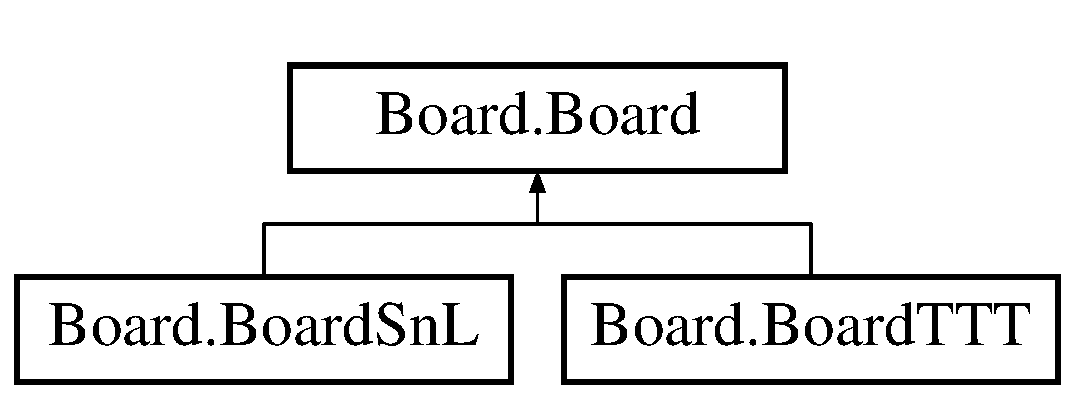
\includegraphics[height=2.000000cm]{class_board_1_1_board}
\end{center}
\end{figure}
\subsection*{Public Member Functions}
\begin{DoxyCompactItemize}
\item 
int \hyperlink{class_board_1_1_board_a2eac3ef13d90ea0dfdc2c198bcab030d}{get\+Board\+Width} ()
\item 
int \hyperlink{class_board_1_1_board_a76b63d4d319e6a0f9f574a3fa8e5d00b}{get\+Board\+Height} ()
\item 
\hyperlink{class_board_1_1_board_a346819dc6f781a6a6c03a2bf8219e1e0}{Board} (int width, int height)
\item 
\hyperlink{class_square_1_1_square}{Square} \hyperlink{class_board_1_1_board_a279f8936c2da2be7c0c12d61212a7591}{access\+Square} (int x, int y)
\item 
\hyperlink{class_square_1_1_square}{Square} \hyperlink{class_board_1_1_board_aa2e9404b4c5fa4b7c22376610f172da8}{access\+Square} (int i)
\item 
abstract int \hyperlink{class_board_1_1_board_a1e4af7a26127d7f715c9df3d058ac97e}{detect\+End\+Game} ()
\end{DoxyCompactItemize}
\subsection*{Protected Attributes}
\begin{DoxyCompactItemize}
\item 
\hyperlink{class_square_1_1_square}{Square}\mbox{[}$\,$\mbox{]} \hyperlink{class_board_1_1_board_aede8ecf481e3981e0ec04d7bd3520bea}{m\+\_\+board\+Game}
\item 
int \hyperlink{class_board_1_1_board_a811ddc59658729b3cdb0a2db75465334}{m\+\_\+board\+Width}
\item 
int \hyperlink{class_board_1_1_board_a4a513d0963fd4e135fac9d121aea3a98}{m\+\_\+board\+Height}
\end{DoxyCompactItemize}


\subsection{Detailed Description}


Definition at line 24 of file Board.\+java.



\subsection{Constructor \& Destructor Documentation}
\hypertarget{class_board_1_1_board_a346819dc6f781a6a6c03a2bf8219e1e0}{}\index{Board\+::\+Board@{Board\+::\+Board}!Board@{Board}}
\index{Board@{Board}!Board\+::\+Board@{Board\+::\+Board}}
\subsubsection[{Board(int width, int height)}]{\setlength{\rightskip}{0pt plus 5cm}Board.\+Board.\+Board (
\begin{DoxyParamCaption}
\item[{int}]{width, }
\item[{int}]{height}
\end{DoxyParamCaption}
)}\label{class_board_1_1_board_a346819dc6f781a6a6c03a2bf8219e1e0}
Constructor for creating a new board 
\begin{DoxyParams}{Parameters}
{\em width} & int containing the width of the board to be created \\
\hline
{\em height} & int containing the height of the board to be created \\
\hline
\end{DoxyParams}


Definition at line 61 of file Board.\+java.



References Menu.\+Game\+Selector.\+m\+\_\+\+T\+R\+A\+C\+E.



\subsection{Member Function Documentation}
\hypertarget{class_board_1_1_board_a279f8936c2da2be7c0c12d61212a7591}{}\index{Board\+::\+Board@{Board\+::\+Board}!access\+Square@{access\+Square}}
\index{access\+Square@{access\+Square}!Board\+::\+Board@{Board\+::\+Board}}
\subsubsection[{access\+Square(int x, int y)}]{\setlength{\rightskip}{0pt plus 5cm}{\bf Square} Board.\+Board.\+access\+Square (
\begin{DoxyParamCaption}
\item[{int}]{x, }
\item[{int}]{y}
\end{DoxyParamCaption}
)}\label{class_board_1_1_board_a279f8936c2da2be7c0c12d61212a7591}
Gives access to a specific square on the board, used for T\+T\+T 
\begin{DoxyParams}{Parameters}
{\em x} & int containing the x position to access \\
\hline
{\em y} & int containing the y position to access \\
\hline
\end{DoxyParams}
\begin{DoxyReturn}{Returns}
Square type containing the information on the square at coordinates (x,y) 
\end{DoxyReturn}


Definition at line 78 of file Board.\+java.



References Menu.\+Game\+Selector.\+m\+\_\+\+T\+R\+A\+C\+E.



Referenced by Display.\+Display\+T\+T\+T.\+ai\+Movement\+Strategy(), Board.\+Board\+T\+T\+T.\+detect\+End\+Game(), Board.\+Board\+Sn\+L.\+detect\+End\+Game(), Display.\+Display\+T\+T\+T.\+save\+Game(), Game.\+Game\+T\+T\+T.\+set\+Movement\+A\+I(), Game.\+Game\+T\+T\+T.\+set\+Movement\+Human(), Board.\+Board\+T\+T\+T.\+win\+Column(), Board.\+Board\+T\+T\+T.\+win\+Diagonal\+Left(), Board.\+Board\+T\+T\+T.\+win\+Diagonal\+Right(), and Board.\+Board\+T\+T\+T.\+win\+Row().

\hypertarget{class_board_1_1_board_aa2e9404b4c5fa4b7c22376610f172da8}{}\index{Board\+::\+Board@{Board\+::\+Board}!access\+Square@{access\+Square}}
\index{access\+Square@{access\+Square}!Board\+::\+Board@{Board\+::\+Board}}
\subsubsection[{access\+Square(int i)}]{\setlength{\rightskip}{0pt plus 5cm}{\bf Square} Board.\+Board.\+access\+Square (
\begin{DoxyParamCaption}
\item[{int}]{i}
\end{DoxyParamCaption}
)}\label{class_board_1_1_board_aa2e9404b4c5fa4b7c22376610f172da8}
Gives access to a specific square on the board, used in Sn\+L 
\begin{DoxyParams}{Parameters}
{\em i} & int containing the position to access \\
\hline
\end{DoxyParams}
\begin{DoxyReturn}{Returns}
Square type containing the information on the square at position i 
\end{DoxyReturn}


Definition at line 92 of file Board.\+java.



References Menu.\+Game\+Selector.\+m\+\_\+\+T\+R\+A\+C\+E.

\hypertarget{class_board_1_1_board_a1e4af7a26127d7f715c9df3d058ac97e}{}\index{Board\+::\+Board@{Board\+::\+Board}!detect\+End\+Game@{detect\+End\+Game}}
\index{detect\+End\+Game@{detect\+End\+Game}!Board\+::\+Board@{Board\+::\+Board}}
\subsubsection[{detect\+End\+Game()}]{\setlength{\rightskip}{0pt plus 5cm}abstract int Board.\+Board.\+detect\+End\+Game (
\begin{DoxyParamCaption}
{}
\end{DoxyParamCaption}
)\hspace{0.3cm}{\ttfamily [abstract]}}\label{class_board_1_1_board_a1e4af7a26127d7f715c9df3d058ac97e}
Used to detect when the end of the game has been reached, Implementation can be found in child classes. \begin{DoxyReturn}{Returns}
int depending on what type of win has been reached 
\end{DoxyReturn}
\hypertarget{class_board_1_1_board_a76b63d4d319e6a0f9f574a3fa8e5d00b}{}\index{Board\+::\+Board@{Board\+::\+Board}!get\+Board\+Height@{get\+Board\+Height}}
\index{get\+Board\+Height@{get\+Board\+Height}!Board\+::\+Board@{Board\+::\+Board}}
\subsubsection[{get\+Board\+Height()}]{\setlength{\rightskip}{0pt plus 5cm}int Board.\+Board.\+get\+Board\+Height (
\begin{DoxyParamCaption}
{}
\end{DoxyParamCaption}
)}\label{class_board_1_1_board_a76b63d4d319e6a0f9f574a3fa8e5d00b}
gets the Heighth of the board \begin{DoxyReturn}{Returns}
int containing the board Height 
\end{DoxyReturn}


Definition at line 48 of file Board.\+java.



References Menu.\+Game\+Selector.\+m\+\_\+\+T\+R\+A\+C\+E.

\hypertarget{class_board_1_1_board_a2eac3ef13d90ea0dfdc2c198bcab030d}{}\index{Board\+::\+Board@{Board\+::\+Board}!get\+Board\+Width@{get\+Board\+Width}}
\index{get\+Board\+Width@{get\+Board\+Width}!Board\+::\+Board@{Board\+::\+Board}}
\subsubsection[{get\+Board\+Width()}]{\setlength{\rightskip}{0pt plus 5cm}int Board.\+Board.\+get\+Board\+Width (
\begin{DoxyParamCaption}
{}
\end{DoxyParamCaption}
)}\label{class_board_1_1_board_a2eac3ef13d90ea0dfdc2c198bcab030d}
gets the width of the board \begin{DoxyReturn}{Returns}
int containing the board width 
\end{DoxyReturn}


Definition at line 36 of file Board.\+java.



References Menu.\+Game\+Selector.\+m\+\_\+\+T\+R\+A\+C\+E.



\subsection{Member Data Documentation}
\hypertarget{class_board_1_1_board_aede8ecf481e3981e0ec04d7bd3520bea}{}\index{Board\+::\+Board@{Board\+::\+Board}!m\+\_\+board\+Game@{m\+\_\+board\+Game}}
\index{m\+\_\+board\+Game@{m\+\_\+board\+Game}!Board\+::\+Board@{Board\+::\+Board}}
\subsubsection[{m\+\_\+board\+Game}]{\setlength{\rightskip}{0pt plus 5cm}{\bf Square} \mbox{[}$\,$\mbox{]} Board.\+Board.\+m\+\_\+board\+Game\hspace{0.3cm}{\ttfamily [protected]}}\label{class_board_1_1_board_aede8ecf481e3981e0ec04d7bd3520bea}
The array that stores all the squares used on the board 

Definition at line 27 of file Board.\+java.



Referenced by Board.\+Board\+T\+T\+T.\+Board\+T\+T\+T().

\hypertarget{class_board_1_1_board_a4a513d0963fd4e135fac9d121aea3a98}{}\index{Board\+::\+Board@{Board\+::\+Board}!m\+\_\+board\+Height@{m\+\_\+board\+Height}}
\index{m\+\_\+board\+Height@{m\+\_\+board\+Height}!Board\+::\+Board@{Board\+::\+Board}}
\subsubsection[{m\+\_\+board\+Height}]{\setlength{\rightskip}{0pt plus 5cm}int Board.\+Board.\+m\+\_\+board\+Height\hspace{0.3cm}{\ttfamily [protected]}}\label{class_board_1_1_board_a4a513d0963fd4e135fac9d121aea3a98}


Definition at line 30 of file Board.\+java.



Referenced by Board.\+Board\+T\+T\+T.\+detect\+End\+Game(), and Board.\+Board\+Sn\+L.\+initialize\+Grid().

\hypertarget{class_board_1_1_board_a811ddc59658729b3cdb0a2db75465334}{}\index{Board\+::\+Board@{Board\+::\+Board}!m\+\_\+board\+Width@{m\+\_\+board\+Width}}
\index{m\+\_\+board\+Width@{m\+\_\+board\+Width}!Board\+::\+Board@{Board\+::\+Board}}
\subsubsection[{m\+\_\+board\+Width}]{\setlength{\rightskip}{0pt plus 5cm}int Board.\+Board.\+m\+\_\+board\+Width\hspace{0.3cm}{\ttfamily [protected]}}\label{class_board_1_1_board_a811ddc59658729b3cdb0a2db75465334}
Variables that store the height and width of the board. 

Definition at line 29 of file Board.\+java.



Referenced by Board.\+Board\+T\+T\+T.\+detect\+End\+Game(), Board.\+Board\+Sn\+L.\+initialize\+Grid(), Board.\+Board\+T\+T\+T.\+win\+Column(), Board.\+Board\+T\+T\+T.\+win\+Diagonal\+Left(), Board.\+Board\+T\+T\+T.\+win\+Diagonal\+Right(), and Board.\+Board\+T\+T\+T.\+win\+Row().



The documentation for this class was generated from the following file\+:\begin{DoxyCompactItemize}
\item 
src/\+Board/\hyperlink{_board_8java}{Board.\+java}\end{DoxyCompactItemize}

\hypertarget{class_board_1_1_board_sn_l}{}\section{Board.\+Board\+Sn\+L Class Reference}
\label{class_board_1_1_board_sn_l}\index{Board.\+Board\+Sn\+L@{Board.\+Board\+Sn\+L}}


the board class for Sn\+L which is a subclass of board, it contains specific methods for the Sn\+L game, such as checking if there is a player on the 100th square  




Inheritance diagram for Board.\+Board\+Sn\+L\+:\nopagebreak
\begin{figure}[H]
\begin{center}
\leavevmode
\includegraphics[width=168pt]{class_board_1_1_board_sn_l__inherit__graph}
\end{center}
\end{figure}


Collaboration diagram for Board.\+Board\+Sn\+L\+:\nopagebreak
\begin{figure}[H]
\begin{center}
\leavevmode
\includegraphics[width=271pt]{class_board_1_1_board_sn_l__coll__graph}
\end{center}
\end{figure}
\subsection*{Public Member Functions}
\begin{DoxyCompactItemize}
\item 
\hyperlink{class_square_1_1_square_sn_l}{Square\+Sn\+L} \hyperlink{class_board_1_1_board_sn_l_a808a8299c5ee4a8256b5e68915fd9eca}{get\+Square} (int i)
\item 
\hyperlink{class_board_1_1_board_sn_l_a03f7b8911496b68ad4de0d1b0939220a}{Board\+Sn\+L} (int width, int height, Array\+List$<$ Integer $>$ movement\+Squares, Array\+List$<$ Integer $>$ ladders\+List, Array\+List$<$ Integer $>$ snakes\+List)
\item 
int \hyperlink{class_board_1_1_board_sn_l_aae2b39e92ddf94fefa4bc86a3bdb6055}{detect\+End\+Game} ()
\end{DoxyCompactItemize}
\subsection*{Static Public Member Functions}
\begin{DoxyCompactItemize}
\item 
static void \hyperlink{class_board_1_1_board_sn_l_a528d4e87b3553f7c0bdb7b5a0a3685d5}{main} (String\mbox{[}$\,$\mbox{]} args)
\end{DoxyCompactItemize}
\subsection*{Protected Member Functions}
\begin{DoxyCompactItemize}
\item 
void \hyperlink{class_board_1_1_board_sn_l_a934454d70accef26911914261147d8f5}{initialize\+Grid} (int width, int height)
\end{DoxyCompactItemize}
\subsection*{Private Attributes}
\begin{DoxyCompactItemize}
\item 
\hyperlink{class_square_1_1_square_sn_l}{Square\+Sn\+L}\mbox{[}$\,$\mbox{]} \hyperlink{class_board_1_1_board_sn_l_a98423adeb63e796de2d496689b4ce8e1}{m\+\_\+board\+Game}
\item 
final int \hyperlink{class_board_1_1_board_sn_l_a133b0d6726fc954ea12a66b4369e3fa6}{F\+I\+N\+A\+L\+\_\+\+S\+Q\+U\+A\+R\+E} = 99
\item 
final int \hyperlink{class_board_1_1_board_sn_l_a9f3b27889e40b337a28438224a5fab4b}{W\+I\+N} = 1
\item 
final int \hyperlink{class_board_1_1_board_sn_l_aa6138411eddcd92ae999cff9fc34acb7}{L\+O\+S\+S} = 0
\end{DoxyCompactItemize}
\subsection*{Additional Inherited Members}


\subsection{Detailed Description}
the board class for Sn\+L which is a subclass of board, it contains specific methods for the Sn\+L game, such as checking if there is a player on the 100th square 

Definition at line 28 of file Board\+Sn\+L.\+java.



\subsection{Constructor \& Destructor Documentation}
\hypertarget{class_board_1_1_board_sn_l_a03f7b8911496b68ad4de0d1b0939220a}{}\index{Board\+::\+Board\+Sn\+L@{Board\+::\+Board\+Sn\+L}!Board\+Sn\+L@{Board\+Sn\+L}}
\index{Board\+Sn\+L@{Board\+Sn\+L}!Board\+::\+Board\+Sn\+L@{Board\+::\+Board\+Sn\+L}}
\subsubsection[{Board\+Sn\+L(int width, int height, Array\+List$<$ Integer $>$ movement\+Squares, Array\+List$<$ Integer $>$ ladders\+List, Array\+List$<$ Integer $>$ snakes\+List)}]{\setlength{\rightskip}{0pt plus 5cm}Board.\+Board\+Sn\+L.\+Board\+Sn\+L (
\begin{DoxyParamCaption}
\item[{int}]{width, }
\item[{int}]{height, }
\item[{Array\+List$<$ Integer $>$}]{movement\+Squares, }
\item[{Array\+List$<$ Integer $>$}]{ladders\+List, }
\item[{Array\+List$<$ Integer $>$}]{snakes\+List}
\end{DoxyParamCaption}
)}\label{class_board_1_1_board_sn_l_a03f7b8911496b68ad4de0d1b0939220a}
Constructor for creating the new board, creates new Squares to fill the board, the number of which is width$\ast$height 
\begin{DoxyParams}{Parameters}
{\em width} & int containing the width of the board to be created \\
\hline
{\em height} & int containing the height of the board to be created \\
\hline
{\em movement\+Squares} & Array\+List of integers containing the position of the ladder bottoms and tail tops (the squares where addition movement occurs) \\
\hline
{\em ladders\+List} & Array\+List of integers containing the positions of both the tops and bottoms of ladders. \\
\hline
{\em snakes\+List} & Array\+List of integers containing the positions of both the tops and bottoms of snakes. \\
\hline
\end{DoxyParams}


Definition at line 68 of file Board\+Sn\+L.\+java.



References Game.\+Game\+Sn\+L.\+get\+Movement\+Pair(), Board.\+Board\+Sn\+L.\+initialize\+Grid(), and Menu.\+Game\+Selector.\+m\+\_\+\+T\+R\+A\+C\+E.



Referenced by Board.\+Board\+Sn\+L.\+main().



\subsection{Member Function Documentation}
\hypertarget{class_board_1_1_board_sn_l_aae2b39e92ddf94fefa4bc86a3bdb6055}{}\index{Board\+::\+Board\+Sn\+L@{Board\+::\+Board\+Sn\+L}!detect\+End\+Game@{detect\+End\+Game}}
\index{detect\+End\+Game@{detect\+End\+Game}!Board\+::\+Board\+Sn\+L@{Board\+::\+Board\+Sn\+L}}
\subsubsection[{detect\+End\+Game()}]{\setlength{\rightskip}{0pt plus 5cm}int Board.\+Board\+Sn\+L.\+detect\+End\+Game (
\begin{DoxyParamCaption}
{}
\end{DoxyParamCaption}
)}\label{class_board_1_1_board_sn_l_aae2b39e92ddf94fefa4bc86a3bdb6055}
Method for detecting whether the end game has been reached \begin{DoxyReturn}{Returns}
int containing 1 if win detected 0 if not. 
\end{DoxyReturn}


Definition at line 112 of file Board\+Sn\+L.\+java.



References Board.\+Board.\+access\+Square(), Board.\+Board\+Sn\+L.\+L\+O\+S\+S, Menu.\+Game\+Selector.\+m\+\_\+\+T\+R\+A\+C\+E, and Board.\+Board\+Sn\+L.\+W\+I\+N.



Referenced by Board.\+Board\+Sn\+L.\+main().

\hypertarget{class_board_1_1_board_sn_l_a808a8299c5ee4a8256b5e68915fd9eca}{}\index{Board\+::\+Board\+Sn\+L@{Board\+::\+Board\+Sn\+L}!get\+Square@{get\+Square}}
\index{get\+Square@{get\+Square}!Board\+::\+Board\+Sn\+L@{Board\+::\+Board\+Sn\+L}}
\subsubsection[{get\+Square(int i)}]{\setlength{\rightskip}{0pt plus 5cm}{\bf Square\+Sn\+L} Board.\+Board\+Sn\+L.\+get\+Square (
\begin{DoxyParamCaption}
\item[{int}]{i}
\end{DoxyParamCaption}
)}\label{class_board_1_1_board_sn_l_a808a8299c5ee4a8256b5e68915fd9eca}
Gives access to a specific square on the board 
\begin{DoxyParams}{Parameters}
{\em i} & int containing the position to access \\
\hline
\end{DoxyParams}
\begin{DoxyReturn}{Returns}
Square\+Sn\+L pointer to the square located at position i 
\end{DoxyReturn}


Definition at line 47 of file Board\+Sn\+L.\+java.



References Menu.\+Game\+Selector.\+m\+\_\+\+T\+R\+A\+C\+E.



Referenced by Game.\+Game\+Sn\+L.\+check\+Move(), Game.\+Game\+Sn\+L.\+main(), and Game.\+Game\+Sn\+L.\+move\+Player().

\hypertarget{class_board_1_1_board_sn_l_a934454d70accef26911914261147d8f5}{}\index{Board\+::\+Board\+Sn\+L@{Board\+::\+Board\+Sn\+L}!initialize\+Grid@{initialize\+Grid}}
\index{initialize\+Grid@{initialize\+Grid}!Board\+::\+Board\+Sn\+L@{Board\+::\+Board\+Sn\+L}}
\subsubsection[{initialize\+Grid(int width, int height)}]{\setlength{\rightskip}{0pt plus 5cm}void Board.\+Board\+Sn\+L.\+initialize\+Grid (
\begin{DoxyParamCaption}
\item[{int}]{width, }
\item[{int}]{height}
\end{DoxyParamCaption}
)\hspace{0.3cm}{\ttfamily [protected]}}\label{class_board_1_1_board_sn_l_a934454d70accef26911914261147d8f5}
Method that initialises the Sn\+L grid with squares ready for their values to be set 
\begin{DoxyParams}{Parameters}
{\em width} & integer containing the width of board to set up \\
\hline
{\em height} & integer containing the height of board to set up \\
\hline
\end{DoxyParams}


Definition at line 98 of file Board\+Sn\+L.\+java.



References Board.\+Board.\+m\+\_\+board\+Height, Board.\+Board.\+m\+\_\+board\+Width, and Menu.\+Game\+Selector.\+m\+\_\+\+T\+R\+A\+C\+E.



Referenced by Board.\+Board\+Sn\+L.\+Board\+Sn\+L().

\hypertarget{class_board_1_1_board_sn_l_a528d4e87b3553f7c0bdb7b5a0a3685d5}{}\index{Board\+::\+Board\+Sn\+L@{Board\+::\+Board\+Sn\+L}!main@{main}}
\index{main@{main}!Board\+::\+Board\+Sn\+L@{Board\+::\+Board\+Sn\+L}}
\subsubsection[{main(\+String[] args)}]{\setlength{\rightskip}{0pt plus 5cm}static void Board.\+Board\+Sn\+L.\+main (
\begin{DoxyParamCaption}
\item[{String\mbox{[}$\,$\mbox{]}}]{args}
\end{DoxyParamCaption}
)\hspace{0.3cm}{\ttfamily [static]}}\label{class_board_1_1_board_sn_l_a528d4e87b3553f7c0bdb7b5a0a3685d5}
Test method 

Definition at line 129 of file Board\+Sn\+L.\+java.



References Board.\+Board\+Sn\+L.\+Board\+Sn\+L(), and Board.\+Board\+Sn\+L.\+detect\+End\+Game().



\subsection{Member Data Documentation}
\hypertarget{class_board_1_1_board_sn_l_a133b0d6726fc954ea12a66b4369e3fa6}{}\index{Board\+::\+Board\+Sn\+L@{Board\+::\+Board\+Sn\+L}!F\+I\+N\+A\+L\+\_\+\+S\+Q\+U\+A\+R\+E@{F\+I\+N\+A\+L\+\_\+\+S\+Q\+U\+A\+R\+E}}
\index{F\+I\+N\+A\+L\+\_\+\+S\+Q\+U\+A\+R\+E@{F\+I\+N\+A\+L\+\_\+\+S\+Q\+U\+A\+R\+E}!Board\+::\+Board\+Sn\+L@{Board\+::\+Board\+Sn\+L}}
\subsubsection[{F\+I\+N\+A\+L\+\_\+\+S\+Q\+U\+A\+R\+E}]{\setlength{\rightskip}{0pt plus 5cm}final int Board.\+Board\+Sn\+L.\+F\+I\+N\+A\+L\+\_\+\+S\+Q\+U\+A\+R\+E = 99\hspace{0.3cm}{\ttfamily [private]}}\label{class_board_1_1_board_sn_l_a133b0d6726fc954ea12a66b4369e3fa6}
An integer storing the final square on the board 

Definition at line 34 of file Board\+Sn\+L.\+java.

\hypertarget{class_board_1_1_board_sn_l_aa6138411eddcd92ae999cff9fc34acb7}{}\index{Board\+::\+Board\+Sn\+L@{Board\+::\+Board\+Sn\+L}!L\+O\+S\+S@{L\+O\+S\+S}}
\index{L\+O\+S\+S@{L\+O\+S\+S}!Board\+::\+Board\+Sn\+L@{Board\+::\+Board\+Sn\+L}}
\subsubsection[{L\+O\+S\+S}]{\setlength{\rightskip}{0pt plus 5cm}final int Board.\+Board\+Sn\+L.\+L\+O\+S\+S = 0\hspace{0.3cm}{\ttfamily [private]}}\label{class_board_1_1_board_sn_l_aa6138411eddcd92ae999cff9fc34acb7}
integer storing return value for the method detect\+End\+Game 

Definition at line 40 of file Board\+Sn\+L.\+java.



Referenced by Board.\+Board\+Sn\+L.\+detect\+End\+Game().

\hypertarget{class_board_1_1_board_sn_l_a98423adeb63e796de2d496689b4ce8e1}{}\index{Board\+::\+Board\+Sn\+L@{Board\+::\+Board\+Sn\+L}!m\+\_\+board\+Game@{m\+\_\+board\+Game}}
\index{m\+\_\+board\+Game@{m\+\_\+board\+Game}!Board\+::\+Board\+Sn\+L@{Board\+::\+Board\+Sn\+L}}
\subsubsection[{m\+\_\+board\+Game}]{\setlength{\rightskip}{0pt plus 5cm}{\bf Square\+Sn\+L} \mbox{[}$\,$\mbox{]} Board.\+Board\+Sn\+L.\+m\+\_\+board\+Game\hspace{0.3cm}{\ttfamily [private]}}\label{class_board_1_1_board_sn_l_a98423adeb63e796de2d496689b4ce8e1}
The array that stores all the squares used on the board 

Definition at line 31 of file Board\+Sn\+L.\+java.

\hypertarget{class_board_1_1_board_sn_l_a9f3b27889e40b337a28438224a5fab4b}{}\index{Board\+::\+Board\+Sn\+L@{Board\+::\+Board\+Sn\+L}!W\+I\+N@{W\+I\+N}}
\index{W\+I\+N@{W\+I\+N}!Board\+::\+Board\+Sn\+L@{Board\+::\+Board\+Sn\+L}}
\subsubsection[{W\+I\+N}]{\setlength{\rightskip}{0pt plus 5cm}final int Board.\+Board\+Sn\+L.\+W\+I\+N = 1\hspace{0.3cm}{\ttfamily [private]}}\label{class_board_1_1_board_sn_l_a9f3b27889e40b337a28438224a5fab4b}
integer storing return value for the method detect\+End\+Game 

Definition at line 37 of file Board\+Sn\+L.\+java.



Referenced by Board.\+Board\+Sn\+L.\+detect\+End\+Game().



The documentation for this class was generated from the following file\+:\begin{DoxyCompactItemize}
\item 
src/\+Board/\hyperlink{_board_sn_l_8java}{Board\+Sn\+L.\+java}\end{DoxyCompactItemize}

\hypertarget{class_board_1_1_board_t_t_t}{}\section{Board.\+Board\+T\+T\+T Class Reference}
\label{class_board_1_1_board_t_t_t}\index{Board.\+Board\+T\+T\+T@{Board.\+Board\+T\+T\+T}}


Specific board class for T\+T\+T game board class for T\+T\+T which is a subclass of board, this subclass contains methods specific to T\+T\+T, such as detecting the win scenario by working out adjacent squares to the players current square.  




Inheritance diagram for Board.\+Board\+T\+T\+T\+:
\nopagebreak
\begin{figure}[H]
\begin{center}
\leavevmode
\includegraphics[width=170pt]{class_board_1_1_board_t_t_t__inherit__graph}
\end{center}
\end{figure}


Collaboration diagram for Board.\+Board\+T\+T\+T\+:
\nopagebreak
\begin{figure}[H]
\begin{center}
\leavevmode
\includegraphics[width=194pt]{class_board_1_1_board_t_t_t__coll__graph}
\end{center}
\end{figure}
\subsection*{Public Member Functions}
\begin{DoxyCompactItemize}
\item 
int\mbox{[}$\,$\mbox{]} \hyperlink{class_board_1_1_board_t_t_t_a14ae6a700a6f83643afd3da120c1ee26}{get\+Coordinates\+Winning\+Squares} ()
\item 
\hyperlink{class_board_1_1_board_t_t_t_ac79a9beb148634225ef350d3ca0628ad}{Board\+T\+T\+T} (int width, int height)
\item 
\hyperlink{class_board_1_1_board_t_t_t_a3a5fc9e11157089f888727ba696fc2e4}{Board\+T\+T\+T} (int width, int height, char\mbox{[}$\,$\mbox{]} square\+Values, \hyperlink{class_display_1_1_display_t_t_t}{Display\+T\+T\+T} display)
\item 
int \hyperlink{class_board_1_1_board_t_t_t_a08f36da4210111d8f129be28a550334e}{detect\+End\+Game} ()
\end{DoxyCompactItemize}
\subsection*{Static Public Member Functions}
\begin{DoxyCompactItemize}
\item 
static void \hyperlink{class_board_1_1_board_t_t_t_a1b62648f4ca1d4a074767027b9c8eec0}{main} (String\mbox{[}$\,$\mbox{]} args)
\end{DoxyCompactItemize}
\subsection*{Static Public Attributes}
\begin{DoxyCompactItemize}
\item 
static final int \hyperlink{class_board_1_1_board_t_t_t_a16be9cbe57d43388a3fa6e5b706210e5}{D\+R\+A\+W\+\_\+\+G\+A\+M\+E} = -\/1
\item 
static final int \hyperlink{class_board_1_1_board_t_t_t_a5448324216e6a32d3264e50779962562}{N\+O\+T\+H\+I\+N\+G\+\_\+\+H\+A\+P\+P\+E\+N\+E\+D} = 0
\item 
static final int \hyperlink{class_board_1_1_board_t_t_t_a989aacd76a6193fe54a4500dd8151b41}{O\+\_\+\+W\+I\+N} = 1
\item 
static final int \hyperlink{class_board_1_1_board_t_t_t_ab77ee706643fb1825e78f6b8dcacc021}{X\+\_\+\+W\+I\+N} = 2
\end{DoxyCompactItemize}
\subsection*{Private Member Functions}
\begin{DoxyCompactItemize}
\item 
Boolean \hyperlink{class_board_1_1_board_t_t_t_ab7d0a91870f300ee5544da2c1ee8b67c}{win} (char Xor\+O)
\item 
Boolean \hyperlink{class_board_1_1_board_t_t_t_adeda4fd9adb536be218a068d71be8587}{win\+Row} (char Xor\+O)
\item 
Boolean \hyperlink{class_board_1_1_board_t_t_t_aa133bbee4e44152b8ba57191475409ab}{win\+Column} (char Xor\+O)
\item 
Boolean \hyperlink{class_board_1_1_board_t_t_t_a756f492a748b6050441c6f821809c40d}{win\+Diagonal\+Right} (char Xor\+O)
\item 
Boolean \hyperlink{class_board_1_1_board_t_t_t_a5f5114b28a09db036e030ec6bb97f189}{win\+Diagonal\+Left} (char Xor\+O)
\end{DoxyCompactItemize}
\subsection*{Private Attributes}
\begin{DoxyCompactItemize}
\item 
int\mbox{[}$\,$\mbox{]} \hyperlink{class_board_1_1_board_t_t_t_a50bc789f0168c29495d4827cca10c89f}{m\+\_\+winning\+Square\+Coordinates} = new int\mbox{[}2\mbox{]}
\item 
final int \hyperlink{class_board_1_1_board_t_t_t_ab11d997e2ea0983b566f23c4685767f6}{W\+I\+N\+\_\+\+A\+M\+O\+U\+N\+T} = 5
\end{DoxyCompactItemize}
\subsection*{Additional Inherited Members}


\subsection{Detailed Description}
Specific board class for T\+T\+T game board class for T\+T\+T which is a subclass of board, this subclass contains methods specific to T\+T\+T, such as detecting the win scenario by working out adjacent squares to the players current square. 

Definition at line 28 of file Board\+T\+T\+T.\+java.



\subsection{Constructor \& Destructor Documentation}
\hypertarget{class_board_1_1_board_t_t_t_ac79a9beb148634225ef350d3ca0628ad}{}\index{Board\+::\+Board\+T\+T\+T@{Board\+::\+Board\+T\+T\+T}!Board\+T\+T\+T@{Board\+T\+T\+T}}
\index{Board\+T\+T\+T@{Board\+T\+T\+T}!Board\+::\+Board\+T\+T\+T@{Board\+::\+Board\+T\+T\+T}}
\subsubsection[{Board\+T\+T\+T(int width, int height)}]{\setlength{\rightskip}{0pt plus 5cm}Board.\+Board\+T\+T\+T.\+Board\+T\+T\+T (
\begin{DoxyParamCaption}
\item[{int}]{width, }
\item[{int}]{height}
\end{DoxyParamCaption}
)}\label{class_board_1_1_board_t_t_t_ac79a9beb148634225ef350d3ca0628ad}
Constructor for creating a board of length width$\ast$height 
\begin{DoxyParams}{Parameters}
{\em width} & integer that contains the width of the board to be created \\
\hline
{\em height} & integer that contains the height of the board to be created \\
\hline
\end{DoxyParams}


Definition at line 63 of file Board\+T\+T\+T.\+java.



References Board.\+Board.\+m\+\_\+board\+Game, and Menu.\+Game\+Selector.\+m\+\_\+\+T\+R\+A\+C\+E.



Referenced by Board.\+Board\+T\+T\+T.\+main().

\hypertarget{class_board_1_1_board_t_t_t_a3a5fc9e11157089f888727ba696fc2e4}{}\index{Board\+::\+Board\+T\+T\+T@{Board\+::\+Board\+T\+T\+T}!Board\+T\+T\+T@{Board\+T\+T\+T}}
\index{Board\+T\+T\+T@{Board\+T\+T\+T}!Board\+::\+Board\+T\+T\+T@{Board\+::\+Board\+T\+T\+T}}
\subsubsection[{Board\+T\+T\+T(int width, int height, char[] square\+Values, Display\+T\+T\+T display)}]{\setlength{\rightskip}{0pt plus 5cm}Board.\+Board\+T\+T\+T.\+Board\+T\+T\+T (
\begin{DoxyParamCaption}
\item[{int}]{width, }
\item[{int}]{height, }
\item[{char\mbox{[}$\,$\mbox{]}}]{square\+Values, }
\item[{{\bf Display\+T\+T\+T}}]{display}
\end{DoxyParamCaption}
)}\label{class_board_1_1_board_t_t_t_a3a5fc9e11157089f888727ba696fc2e4}


Definition at line 75 of file Board\+T\+T\+T.\+java.



References Board.\+Board.\+m\+\_\+board\+Game, and Menu.\+Game\+Selector.\+m\+\_\+\+T\+R\+A\+C\+E.



\subsection{Member Function Documentation}
\hypertarget{class_board_1_1_board_t_t_t_a08f36da4210111d8f129be28a550334e}{}\index{Board\+::\+Board\+T\+T\+T@{Board\+::\+Board\+T\+T\+T}!detect\+End\+Game@{detect\+End\+Game}}
\index{detect\+End\+Game@{detect\+End\+Game}!Board\+::\+Board\+T\+T\+T@{Board\+::\+Board\+T\+T\+T}}
\subsubsection[{detect\+End\+Game()}]{\setlength{\rightskip}{0pt plus 5cm}int Board.\+Board\+T\+T\+T.\+detect\+End\+Game (
\begin{DoxyParamCaption}
{}
\end{DoxyParamCaption}
)}\label{class_board_1_1_board_t_t_t_a08f36da4210111d8f129be28a550334e}
First checks for a draw game by looping though every square and checking if there are any empty squares, if there is not then the game is a draw. It then calls the \hyperlink{class_board_1_1_board_t_t_t_ab7d0a91870f300ee5544da2c1ee8b67c}{win()} method on both X and O 

Definition at line 93 of file Board\+T\+T\+T.\+java.



References Board.\+Board.\+access\+Square(), Board.\+Board\+T\+T\+T.\+D\+R\+A\+W\+\_\+\+G\+A\+M\+E, Board.\+Board.\+m\+\_\+board\+Height, Board.\+Board.\+m\+\_\+board\+Width, Menu.\+Game\+Selector.\+m\+\_\+\+T\+R\+A\+C\+E, Board.\+Board\+T\+T\+T.\+N\+O\+T\+H\+I\+N\+G\+\_\+\+H\+A\+P\+P\+E\+N\+E\+D, Board.\+Board\+T\+T\+T.\+O\+\_\+\+W\+I\+N, Board.\+Board\+T\+T\+T.\+win(), and Board.\+Board\+T\+T\+T.\+X\+\_\+\+W\+I\+N.



Referenced by Board.\+Board\+T\+T\+T.\+main(), and Game.\+Game\+T\+T\+T.\+winner().

\hypertarget{class_board_1_1_board_t_t_t_a14ae6a700a6f83643afd3da120c1ee26}{}\index{Board\+::\+Board\+T\+T\+T@{Board\+::\+Board\+T\+T\+T}!get\+Coordinates\+Winning\+Squares@{get\+Coordinates\+Winning\+Squares}}
\index{get\+Coordinates\+Winning\+Squares@{get\+Coordinates\+Winning\+Squares}!Board\+::\+Board\+T\+T\+T@{Board\+::\+Board\+T\+T\+T}}
\subsubsection[{get\+Coordinates\+Winning\+Squares()}]{\setlength{\rightskip}{0pt plus 5cm}int \mbox{[}$\,$\mbox{]} Board.\+Board\+T\+T\+T.\+get\+Coordinates\+Winning\+Squares (
\begin{DoxyParamCaption}
{}
\end{DoxyParamCaption}
)}\label{class_board_1_1_board_t_t_t_a14ae6a700a6f83643afd3da120c1ee26}
Used to return the start and end of the winning chain for output. \begin{DoxyReturn}{Returns}
integer array containing the start and end of the winning chain 
\end{DoxyReturn}


Definition at line 49 of file Board\+T\+T\+T.\+java.



References Menu.\+Game\+Selector.\+m\+\_\+\+T\+R\+A\+C\+E, and Board.\+Board\+T\+T\+T.\+m\+\_\+winning\+Square\+Coordinates.



Referenced by Game.\+Game\+T\+T\+T.\+get\+Coordinates\+Winning\+Squares().

\hypertarget{class_board_1_1_board_t_t_t_a1b62648f4ca1d4a074767027b9c8eec0}{}\index{Board\+::\+Board\+T\+T\+T@{Board\+::\+Board\+T\+T\+T}!main@{main}}
\index{main@{main}!Board\+::\+Board\+T\+T\+T@{Board\+::\+Board\+T\+T\+T}}
\subsubsection[{main(\+String[] args)}]{\setlength{\rightskip}{0pt plus 5cm}static void Board.\+Board\+T\+T\+T.\+main (
\begin{DoxyParamCaption}
\item[{String\mbox{[}$\,$\mbox{]}}]{args}
\end{DoxyParamCaption}
)\hspace{0.3cm}{\ttfamily [static]}}\label{class_board_1_1_board_t_t_t_a1b62648f4ca1d4a074767027b9c8eec0}


Definition at line 351 of file Board\+T\+T\+T.\+java.



References Board.\+Board\+T\+T\+T.\+Board\+T\+T\+T(), Board.\+Board\+T\+T\+T.\+detect\+End\+Game(), and Board.\+Board\+T\+T\+T.\+win().

\hypertarget{class_board_1_1_board_t_t_t_ab7d0a91870f300ee5544da2c1ee8b67c}{}\index{Board\+::\+Board\+T\+T\+T@{Board\+::\+Board\+T\+T\+T}!win@{win}}
\index{win@{win}!Board\+::\+Board\+T\+T\+T@{Board\+::\+Board\+T\+T\+T}}
\subsubsection[{win(char Xor\+O)}]{\setlength{\rightskip}{0pt plus 5cm}Boolean Board.\+Board\+T\+T\+T.\+win (
\begin{DoxyParamCaption}
\item[{char}]{Xor\+O}
\end{DoxyParamCaption}
)\hspace{0.3cm}{\ttfamily [private]}}\label{class_board_1_1_board_t_t_t_ab7d0a91870f300ee5544da2c1ee8b67c}
Checks (horizontally, vertically and then diagonally) if there are five Xs or Os (depending on the input) in a row. 
\begin{DoxyParams}{Parameters}
{\em Xor\+O} & char containing X or O depending on what type of piece to check win for \\
\hline
\end{DoxyParams}
\begin{DoxyReturn}{Returns}
true of false depending on if a win is found. 
\end{DoxyReturn}


Definition at line 136 of file Board\+T\+T\+T.\+java.



References Menu.\+Game\+Selector.\+m\+\_\+\+T\+R\+A\+C\+E, Board.\+Board\+T\+T\+T.\+win\+Column(), Board.\+Board\+T\+T\+T.\+win\+Diagonal\+Left(), Board.\+Board\+T\+T\+T.\+win\+Diagonal\+Right(), and Board.\+Board\+T\+T\+T.\+win\+Row().



Referenced by Board.\+Board\+T\+T\+T.\+detect\+End\+Game(), and Board.\+Board\+T\+T\+T.\+main().

\hypertarget{class_board_1_1_board_t_t_t_aa133bbee4e44152b8ba57191475409ab}{}\index{Board\+::\+Board\+T\+T\+T@{Board\+::\+Board\+T\+T\+T}!win\+Column@{win\+Column}}
\index{win\+Column@{win\+Column}!Board\+::\+Board\+T\+T\+T@{Board\+::\+Board\+T\+T\+T}}
\subsubsection[{win\+Column(char Xor\+O)}]{\setlength{\rightskip}{0pt plus 5cm}Boolean Board.\+Board\+T\+T\+T.\+win\+Column (
\begin{DoxyParamCaption}
\item[{char}]{Xor\+O}
\end{DoxyParamCaption}
)\hspace{0.3cm}{\ttfamily [private]}}\label{class_board_1_1_board_t_t_t_aa133bbee4e44152b8ba57191475409ab}
Checks if there is a vertical win 
\begin{DoxyParams}{Parameters}
{\em Xor\+O} & the char it is checking for \\
\hline
\end{DoxyParams}
\begin{DoxyReturn}{Returns}
true if win is found, false if not 
\end{DoxyReturn}


Definition at line 214 of file Board\+T\+T\+T.\+java.



References Board.\+Board.\+access\+Square(), Display.\+Display\+T\+T\+T.\+G\+R\+I\+D\+\_\+\+H\+E\+I\+G\+H\+T, Display.\+Display\+T\+T\+T.\+G\+R\+I\+D\+\_\+\+W\+I\+D\+T\+H, Board.\+Board.\+m\+\_\+board\+Width, and Menu.\+Game\+Selector.\+m\+\_\+\+T\+R\+A\+C\+E.



Referenced by Board.\+Board\+T\+T\+T.\+win().

\hypertarget{class_board_1_1_board_t_t_t_a5f5114b28a09db036e030ec6bb97f189}{}\index{Board\+::\+Board\+T\+T\+T@{Board\+::\+Board\+T\+T\+T}!win\+Diagonal\+Left@{win\+Diagonal\+Left}}
\index{win\+Diagonal\+Left@{win\+Diagonal\+Left}!Board\+::\+Board\+T\+T\+T@{Board\+::\+Board\+T\+T\+T}}
\subsubsection[{win\+Diagonal\+Left(char Xor\+O)}]{\setlength{\rightskip}{0pt plus 5cm}Boolean Board.\+Board\+T\+T\+T.\+win\+Diagonal\+Left (
\begin{DoxyParamCaption}
\item[{char}]{Xor\+O}
\end{DoxyParamCaption}
)\hspace{0.3cm}{\ttfamily [private]}}\label{class_board_1_1_board_t_t_t_a5f5114b28a09db036e030ec6bb97f189}
Checks if there is a diagonal left win 
\begin{DoxyParams}{Parameters}
{\em Xor\+O} & the char it is checking for \\
\hline
\end{DoxyParams}
\begin{DoxyReturn}{Returns}
true if win is found, false if not 
\end{DoxyReturn}


Definition at line 305 of file Board\+T\+T\+T.\+java.



References Board.\+Board.\+access\+Square(), Display.\+Display\+T\+T\+T.\+G\+R\+I\+D\+\_\+\+H\+E\+I\+G\+H\+T, Display.\+Display\+T\+T\+T.\+G\+R\+I\+D\+\_\+\+W\+I\+D\+T\+H, Board.\+Board.\+m\+\_\+board\+Width, and Menu.\+Game\+Selector.\+m\+\_\+\+T\+R\+A\+C\+E.



Referenced by Board.\+Board\+T\+T\+T.\+win().

\hypertarget{class_board_1_1_board_t_t_t_a756f492a748b6050441c6f821809c40d}{}\index{Board\+::\+Board\+T\+T\+T@{Board\+::\+Board\+T\+T\+T}!win\+Diagonal\+Right@{win\+Diagonal\+Right}}
\index{win\+Diagonal\+Right@{win\+Diagonal\+Right}!Board\+::\+Board\+T\+T\+T@{Board\+::\+Board\+T\+T\+T}}
\subsubsection[{win\+Diagonal\+Right(char Xor\+O)}]{\setlength{\rightskip}{0pt plus 5cm}Boolean Board.\+Board\+T\+T\+T.\+win\+Diagonal\+Right (
\begin{DoxyParamCaption}
\item[{char}]{Xor\+O}
\end{DoxyParamCaption}
)\hspace{0.3cm}{\ttfamily [private]}}\label{class_board_1_1_board_t_t_t_a756f492a748b6050441c6f821809c40d}
Checks if there is a diagonal right win 
\begin{DoxyParams}{Parameters}
{\em Xor\+O} & the char it is checking for \\
\hline
\end{DoxyParams}
\begin{DoxyReturn}{Returns}
true if win is found, false if not 
\end{DoxyReturn}


Definition at line 253 of file Board\+T\+T\+T.\+java.



References Board.\+Board.\+access\+Square(), Display.\+Display\+T\+T\+T.\+G\+R\+I\+D\+\_\+\+H\+E\+I\+G\+H\+T, Display.\+Display\+T\+T\+T.\+G\+R\+I\+D\+\_\+\+W\+I\+D\+T\+H, Board.\+Board.\+m\+\_\+board\+Width, and Menu.\+Game\+Selector.\+m\+\_\+\+T\+R\+A\+C\+E.



Referenced by Board.\+Board\+T\+T\+T.\+win().

\hypertarget{class_board_1_1_board_t_t_t_adeda4fd9adb536be218a068d71be8587}{}\index{Board\+::\+Board\+T\+T\+T@{Board\+::\+Board\+T\+T\+T}!win\+Row@{win\+Row}}
\index{win\+Row@{win\+Row}!Board\+::\+Board\+T\+T\+T@{Board\+::\+Board\+T\+T\+T}}
\subsubsection[{win\+Row(char Xor\+O)}]{\setlength{\rightskip}{0pt plus 5cm}Boolean Board.\+Board\+T\+T\+T.\+win\+Row (
\begin{DoxyParamCaption}
\item[{char}]{Xor\+O}
\end{DoxyParamCaption}
)\hspace{0.3cm}{\ttfamily [private]}}\label{class_board_1_1_board_t_t_t_adeda4fd9adb536be218a068d71be8587}
Checks if there is a horizontal win 
\begin{DoxyParams}{Parameters}
{\em Xor\+O} & the char it is checking for \\
\hline
\end{DoxyParams}
\begin{DoxyReturn}{Returns}
true if win is found, false if not 
\end{DoxyReturn}


Definition at line 176 of file Board\+T\+T\+T.\+java.



References Board.\+Board.\+access\+Square(), Display.\+Display\+T\+T\+T.\+G\+R\+I\+D\+\_\+\+H\+E\+I\+G\+H\+T, Display.\+Display\+T\+T\+T.\+G\+R\+I\+D\+\_\+\+W\+I\+D\+T\+H, Board.\+Board.\+m\+\_\+board\+Width, and Menu.\+Game\+Selector.\+m\+\_\+\+T\+R\+A\+C\+E.



Referenced by Board.\+Board\+T\+T\+T.\+win().



\subsection{Member Data Documentation}
\hypertarget{class_board_1_1_board_t_t_t_a16be9cbe57d43388a3fa6e5b706210e5}{}\index{Board\+::\+Board\+T\+T\+T@{Board\+::\+Board\+T\+T\+T}!D\+R\+A\+W\+\_\+\+G\+A\+M\+E@{D\+R\+A\+W\+\_\+\+G\+A\+M\+E}}
\index{D\+R\+A\+W\+\_\+\+G\+A\+M\+E@{D\+R\+A\+W\+\_\+\+G\+A\+M\+E}!Board\+::\+Board\+T\+T\+T@{Board\+::\+Board\+T\+T\+T}}
\subsubsection[{D\+R\+A\+W\+\_\+\+G\+A\+M\+E}]{\setlength{\rightskip}{0pt plus 5cm}final int Board.\+Board\+T\+T\+T.\+D\+R\+A\+W\+\_\+\+G\+A\+M\+E = -\/1\hspace{0.3cm}{\ttfamily [static]}}\label{class_board_1_1_board_t_t_t_a16be9cbe57d43388a3fa6e5b706210e5}
integers that store the return values for \hyperlink{class_board_1_1_board_t_t_t_a08f36da4210111d8f129be28a550334e}{detect\+End\+Game()} 

Definition at line 38 of file Board\+T\+T\+T.\+java.



Referenced by Board.\+Board\+T\+T\+T.\+detect\+End\+Game().

\hypertarget{class_board_1_1_board_t_t_t_a50bc789f0168c29495d4827cca10c89f}{}\index{Board\+::\+Board\+T\+T\+T@{Board\+::\+Board\+T\+T\+T}!m\+\_\+winning\+Square\+Coordinates@{m\+\_\+winning\+Square\+Coordinates}}
\index{m\+\_\+winning\+Square\+Coordinates@{m\+\_\+winning\+Square\+Coordinates}!Board\+::\+Board\+T\+T\+T@{Board\+::\+Board\+T\+T\+T}}
\subsubsection[{m\+\_\+winning\+Square\+Coordinates}]{\setlength{\rightskip}{0pt plus 5cm}int \mbox{[}$\,$\mbox{]} Board.\+Board\+T\+T\+T.\+m\+\_\+winning\+Square\+Coordinates = new int\mbox{[}2\mbox{]}\hspace{0.3cm}{\ttfamily [private]}}\label{class_board_1_1_board_t_t_t_a50bc789f0168c29495d4827cca10c89f}
Integer array used to store the start and end of the winning chain for output 

Definition at line 33 of file Board\+T\+T\+T.\+java.



Referenced by Board.\+Board\+T\+T\+T.\+get\+Coordinates\+Winning\+Squares().

\hypertarget{class_board_1_1_board_t_t_t_a5448324216e6a32d3264e50779962562}{}\index{Board\+::\+Board\+T\+T\+T@{Board\+::\+Board\+T\+T\+T}!N\+O\+T\+H\+I\+N\+G\+\_\+\+H\+A\+P\+P\+E\+N\+E\+D@{N\+O\+T\+H\+I\+N\+G\+\_\+\+H\+A\+P\+P\+E\+N\+E\+D}}
\index{N\+O\+T\+H\+I\+N\+G\+\_\+\+H\+A\+P\+P\+E\+N\+E\+D@{N\+O\+T\+H\+I\+N\+G\+\_\+\+H\+A\+P\+P\+E\+N\+E\+D}!Board\+::\+Board\+T\+T\+T@{Board\+::\+Board\+T\+T\+T}}
\subsubsection[{N\+O\+T\+H\+I\+N\+G\+\_\+\+H\+A\+P\+P\+E\+N\+E\+D}]{\setlength{\rightskip}{0pt plus 5cm}final int Board.\+Board\+T\+T\+T.\+N\+O\+T\+H\+I\+N\+G\+\_\+\+H\+A\+P\+P\+E\+N\+E\+D = 0\hspace{0.3cm}{\ttfamily [static]}}\label{class_board_1_1_board_t_t_t_a5448324216e6a32d3264e50779962562}


Definition at line 39 of file Board\+T\+T\+T.\+java.



Referenced by Board.\+Board\+T\+T\+T.\+detect\+End\+Game().

\hypertarget{class_board_1_1_board_t_t_t_a989aacd76a6193fe54a4500dd8151b41}{}\index{Board\+::\+Board\+T\+T\+T@{Board\+::\+Board\+T\+T\+T}!O\+\_\+\+W\+I\+N@{O\+\_\+\+W\+I\+N}}
\index{O\+\_\+\+W\+I\+N@{O\+\_\+\+W\+I\+N}!Board\+::\+Board\+T\+T\+T@{Board\+::\+Board\+T\+T\+T}}
\subsubsection[{O\+\_\+\+W\+I\+N}]{\setlength{\rightskip}{0pt plus 5cm}final int Board.\+Board\+T\+T\+T.\+O\+\_\+\+W\+I\+N = 1\hspace{0.3cm}{\ttfamily [static]}}\label{class_board_1_1_board_t_t_t_a989aacd76a6193fe54a4500dd8151b41}


Definition at line 40 of file Board\+T\+T\+T.\+java.



Referenced by Board.\+Board\+T\+T\+T.\+detect\+End\+Game().

\hypertarget{class_board_1_1_board_t_t_t_ab11d997e2ea0983b566f23c4685767f6}{}\index{Board\+::\+Board\+T\+T\+T@{Board\+::\+Board\+T\+T\+T}!W\+I\+N\+\_\+\+A\+M\+O\+U\+N\+T@{W\+I\+N\+\_\+\+A\+M\+O\+U\+N\+T}}
\index{W\+I\+N\+\_\+\+A\+M\+O\+U\+N\+T@{W\+I\+N\+\_\+\+A\+M\+O\+U\+N\+T}!Board\+::\+Board\+T\+T\+T@{Board\+::\+Board\+T\+T\+T}}
\subsubsection[{W\+I\+N\+\_\+\+A\+M\+O\+U\+N\+T}]{\setlength{\rightskip}{0pt plus 5cm}final int Board.\+Board\+T\+T\+T.\+W\+I\+N\+\_\+\+A\+M\+O\+U\+N\+T = 5\hspace{0.3cm}{\ttfamily [private]}}\label{class_board_1_1_board_t_t_t_ab11d997e2ea0983b566f23c4685767f6}
integer that stores the length of the chain needed to win 

Definition at line 35 of file Board\+T\+T\+T.\+java.

\hypertarget{class_board_1_1_board_t_t_t_ab77ee706643fb1825e78f6b8dcacc021}{}\index{Board\+::\+Board\+T\+T\+T@{Board\+::\+Board\+T\+T\+T}!X\+\_\+\+W\+I\+N@{X\+\_\+\+W\+I\+N}}
\index{X\+\_\+\+W\+I\+N@{X\+\_\+\+W\+I\+N}!Board\+::\+Board\+T\+T\+T@{Board\+::\+Board\+T\+T\+T}}
\subsubsection[{X\+\_\+\+W\+I\+N}]{\setlength{\rightskip}{0pt plus 5cm}final int Board.\+Board\+T\+T\+T.\+X\+\_\+\+W\+I\+N = 2\hspace{0.3cm}{\ttfamily [static]}}\label{class_board_1_1_board_t_t_t_ab77ee706643fb1825e78f6b8dcacc021}


Definition at line 41 of file Board\+T\+T\+T.\+java.



Referenced by Board.\+Board\+T\+T\+T.\+detect\+End\+Game().



The documentation for this class was generated from the following file\+:\begin{DoxyCompactItemize}
\item 
src/\+Board/\hyperlink{_board_t_t_t_8java}{Board\+T\+T\+T.\+java}\end{DoxyCompactItemize}

\hypertarget{class_display_1_1_display}{}\section{Display.\+Display Class Reference}
\label{class_display_1_1_display}\index{Display.\+Display@{Display.\+Display}}
Inheritance diagram for Display.\+Display\+:\begin{figure}[H]
\begin{center}
\leavevmode
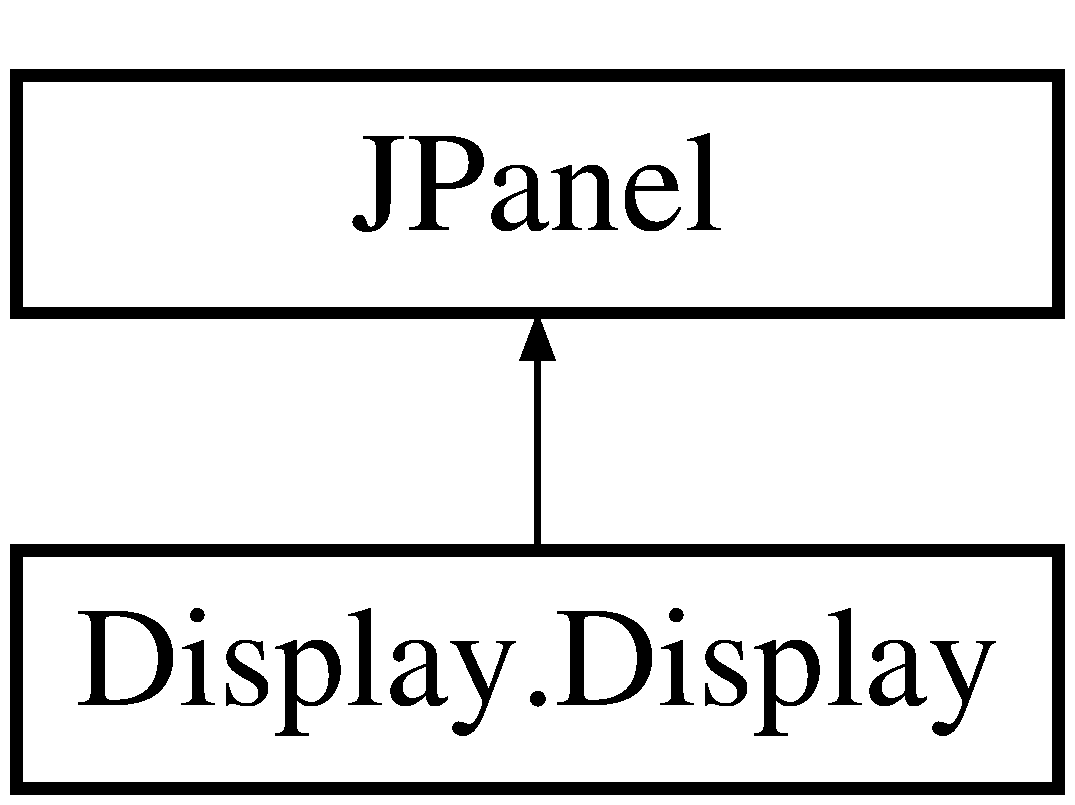
\includegraphics[height=2.000000cm]{class_display_1_1_display}
\end{center}
\end{figure}
\subsection*{Public Member Functions}
\begin{DoxyCompactItemize}
\item 
void \hyperlink{class_display_1_1_display_af117c5499fbaada7683424523b9f333f}{paint\+Component} (Graphics graphics)
\end{DoxyCompactItemize}
\subsection*{Static Public Attributes}
\begin{DoxyCompactItemize}
\item 
static final int \hyperlink{class_display_1_1_display_a044af84b350b1be71c612ab3b534e24d}{X\+P\+O\+S\+\_\+\+C\+O\+L50} = 50
\item 
static final int \hyperlink{class_display_1_1_display_a0a8b9027490d3aa7d66834c6c12c0d35}{X\+P\+O\+S\+\_\+\+C\+O\+L100} = 100
\item 
static final int \hyperlink{class_display_1_1_display_abc29a83a5afef24b6775c0c867d5ca2e}{X\+P\+O\+S\+\_\+\+C\+O\+L150} = 150
\item 
static final int \hyperlink{class_display_1_1_display_adbcb46204650409d834ab66950cdc370}{X\+P\+O\+S\+\_\+\+C\+O\+L200} = 200
\item 
static final int \hyperlink{class_display_1_1_display_a9bc5732eb1a6077901a5e66984ffa339}{X\+P\+O\+S\+\_\+\+C\+O\+L250} = 250
\item 
static final int \hyperlink{class_display_1_1_display_a37098506cf494cbf79cc2ca5e88cd3ac}{X\+P\+O\+S\+\_\+\+C\+O\+L300} = 300
\item 
static final int \hyperlink{class_display_1_1_display_ac0e291caffea8a2d26755c36464c8418}{X\+P\+O\+S\+\_\+\+C\+O\+L350} = 350
\item 
static final int \hyperlink{class_display_1_1_display_a2b04669828dc32ce7435f60985fb9e15}{X\+P\+O\+S\+\_\+\+C\+O\+L400} = 400
\item 
static final int \hyperlink{class_display_1_1_display_aaa4a147d3ae20ff69293868c15b0810c}{X\+P\+O\+S\+\_\+\+C\+O\+L450} = 450
\item 
static final int \hyperlink{class_display_1_1_display_a8fafcc6bf1485ea9d420d3ec725472a7}{X\+P\+O\+S\+\_\+\+C\+O\+L500} = 500
\item 
static final int \hyperlink{class_display_1_1_display_a50de34dab11aef2aa13d782d088deb7d}{X\+P\+O\+S\+\_\+\+C\+O\+L550} = 550
\item 
static final int \hyperlink{class_display_1_1_display_abfcff615e1843cea5f5f5236f7270469}{Y\+P\+O\+S\+\_\+\+R\+O\+W50} = 50
\item 
static final int \hyperlink{class_display_1_1_display_ab910e7da741fb624b211994905f5a1ec}{Y\+P\+O\+S\+\_\+\+R\+O\+W100} = 100
\item 
static final int \hyperlink{class_display_1_1_display_a38a83d9cebcb54826379194267a2ab4a}{Y\+P\+O\+S\+\_\+\+R\+O\+W150} = 150
\item 
static final int \hyperlink{class_display_1_1_display_af186989bbcc82bddc811ce9727cb1d4d}{Y\+P\+O\+S\+\_\+\+R\+O\+W200} = 200
\item 
static final int \hyperlink{class_display_1_1_display_a76fe305a0d851cc121da69952ee13b00}{Y\+P\+O\+S\+\_\+\+R\+O\+W250} = 250
\item 
static final int \hyperlink{class_display_1_1_display_aaf16f1b813645dc5969d6547d7947b3a}{Y\+P\+O\+S\+\_\+\+R\+O\+W300} = 300
\item 
static final int \hyperlink{class_display_1_1_display_ad479e849d0564e40118e7d76652d9ffa}{Y\+P\+O\+S\+\_\+\+R\+O\+W350} = 350
\item 
static final int \hyperlink{class_display_1_1_display_a30efc4ca7cf960942741ac557862fbc8}{Y\+P\+O\+S\+\_\+\+R\+O\+W400} = 400
\item 
static final int \hyperlink{class_display_1_1_display_a68978a2870b55dbd8b5ab6d93db2ed79}{Y\+P\+O\+S\+\_\+\+R\+O\+W450} = 450
\item 
static final int \hyperlink{class_display_1_1_display_af69167585902297bf72bccb89eac59ad}{Y\+P\+O\+S\+\_\+\+R\+O\+W500} = 500
\item 
static final int \hyperlink{class_display_1_1_display_a18e8f506bdeb1ffce18d4e17eacfc1c9}{Y\+P\+O\+S\+\_\+\+R\+O\+W550} = 550
\item 
static final int \hyperlink{class_display_1_1_display_aeb7358eb4ef9314e129e3636eaee48b2}{Y\+P\+O\+S\+\_\+\+R\+O\+W600} = 600
\item 
static final int \hyperlink{class_display_1_1_display_a60296fc1277e58422d02f8f462ad95c5}{Y\+P\+O\+S\+\_\+\+R\+O\+W650} = 650
\item 
static final int \hyperlink{class_display_1_1_display_af02e2130bca24f14a40c4d5c15712b94}{C\+O\+M\+P\+O\+N\+E\+N\+T\+\_\+\+W\+I\+D\+T\+H20} = 20
\item 
static final int \hyperlink{class_display_1_1_display_abad2084dbebbb332775a53c5a79fb055}{C\+O\+M\+P\+O\+N\+E\+N\+T\+\_\+\+W\+I\+D\+T\+H50} = 50
\item 
static final int \hyperlink{class_display_1_1_display_a357b313cc7372c3fce2808f738c26369}{C\+O\+M\+P\+O\+N\+E\+N\+T\+\_\+\+W\+I\+D\+T\+H75} = 75
\item 
static final int \hyperlink{class_display_1_1_display_a42b05e8c9ef5a9a34a30dd19412e22e0}{C\+O\+M\+P\+O\+N\+E\+N\+T\+\_\+\+W\+I\+D\+T\+H80} = 80
\item 
static final int \hyperlink{class_display_1_1_display_a4cb90de4566da894b505b11cf51781ae}{C\+O\+M\+P\+O\+N\+E\+N\+T\+\_\+\+W\+I\+D\+T\+H100} = 100
\item 
static final int \hyperlink{class_display_1_1_display_ad5f14126c874c231b67965c6cdf06178}{C\+O\+M\+P\+O\+N\+E\+N\+T\+\_\+\+W\+I\+D\+T\+H130} = 130
\item 
static final int \hyperlink{class_display_1_1_display_a5684ec094f44cab075327577819190b9}{C\+O\+M\+P\+O\+N\+E\+N\+T\+\_\+\+W\+I\+D\+T\+H150} = 150
\item 
static final int \hyperlink{class_display_1_1_display_a86c529803c94d29b77776f4f56c85f14}{C\+O\+M\+P\+O\+N\+E\+N\+T\+\_\+\+W\+I\+D\+T\+H160} = 160
\item 
static final int \hyperlink{class_display_1_1_display_a8871b58d3f57d5b573779d8af759b7e3}{C\+O\+M\+P\+O\+N\+E\+N\+T\+\_\+\+W\+I\+D\+T\+H170} = 170
\item 
static final int \hyperlink{class_display_1_1_display_a2095098cda35e726fe595b019d78da96}{C\+O\+M\+P\+O\+N\+E\+N\+T\+\_\+\+W\+I\+D\+T\+H175} = 175
\item 
static final int \hyperlink{class_display_1_1_display_a4e3ec7ce466aae4eae284ff350b11253}{C\+O\+M\+P\+O\+N\+E\+N\+T\+\_\+\+W\+I\+D\+T\+H180} = 180
\item 
static final int \hyperlink{class_display_1_1_display_aa5010ddecefd4e39f45361172619b461}{C\+O\+M\+P\+O\+N\+E\+N\+T\+\_\+\+W\+I\+D\+T\+H200} = 200
\item 
static final int \hyperlink{class_display_1_1_display_a4e1ace15de5d4dd0aeb2af46c76742dd}{C\+O\+M\+P\+O\+N\+E\+N\+T\+\_\+\+W\+I\+D\+T\+H250} = 250
\item 
static final int \hyperlink{class_display_1_1_display_a2f111222b6c7d15359547d6f2cbcb01e}{C\+O\+M\+P\+O\+N\+E\+N\+T\+\_\+\+W\+I\+D\+T\+H300} = 300
\item 
static final int \hyperlink{class_display_1_1_display_a63262d6fdb082de5ca713249b0df7703}{C\+O\+M\+P\+O\+N\+E\+N\+T\+\_\+\+W\+I\+D\+T\+H350} = 350
\item 
static final int \hyperlink{class_display_1_1_display_a205927f3e051ee88782c185b37c9e1d5}{C\+O\+M\+P\+O\+N\+E\+N\+T\+\_\+\+H\+E\+I\+G\+H\+T20} = 20
\item 
static final int \hyperlink{class_display_1_1_display_a35a9ab87eca962392fe25c040f594824}{C\+O\+M\+P\+O\+N\+E\+N\+T\+\_\+\+H\+E\+I\+G\+H\+T40} = 40
\item 
static final int \hyperlink{class_display_1_1_display_a3d4ecbb587bdb35ff4e27f0ce4f35e4a}{C\+O\+M\+P\+O\+N\+E\+N\+T\+\_\+\+H\+E\+I\+G\+H\+T50} = 50
\item 
static final int \hyperlink{class_display_1_1_display_afc9a9d568180083ccf2c38b28d908803}{C\+O\+M\+P\+O\+N\+E\+N\+T\+\_\+\+H\+E\+I\+G\+H\+T70} = 70
\item 
static final int \hyperlink{class_display_1_1_display_a4c13bfab8bd26ca8047bef940fae492c}{C\+O\+M\+P\+O\+N\+E\+N\+T\+\_\+\+H\+E\+I\+G\+H\+T80} = 80
\item 
static final int \hyperlink{class_display_1_1_display_a6e40ee081336c35e765e4e880d4e5d8b}{C\+O\+M\+P\+O\+N\+E\+N\+T\+\_\+\+H\+E\+I\+G\+H\+T85} = 85
\item 
static final int \hyperlink{class_display_1_1_display_ad07d0c4e939eca556947af196fd4b6a0}{C\+O\+M\+P\+O\+N\+E\+N\+T\+\_\+\+H\+E\+I\+G\+H\+T100} = 100
\item 
static final int \hyperlink{class_display_1_1_display_aee9bc1bb183f9dfc04267a7cdca2b524}{C\+O\+M\+P\+O\+N\+E\+N\+T\+\_\+\+H\+E\+I\+G\+H\+T150} = 150
\item 
static final int \hyperlink{class_display_1_1_display_a880d1f86d07c77332fa8015e1b7a5145}{C\+O\+M\+P\+O\+N\+E\+N\+T\+\_\+\+H\+E\+I\+G\+H\+T200} = 200
\item 
static final int \hyperlink{class_display_1_1_display_afbd2f610599f4393a4c30314c28ab73b}{C\+O\+M\+P\+O\+N\+E\+N\+T\+\_\+\+H\+E\+I\+G\+H\+T250} = 250
\item 
static final int \hyperlink{class_display_1_1_display_a265426fc52f9fc0f3cf08691bf8fc8bc}{O\+F\+F\+S\+E\+T5} = 5
\item 
static final int \hyperlink{class_display_1_1_display_a43bf93ef0872de87948d181590683656}{O\+F\+F\+S\+E\+T10} = 10
\item 
static final int \hyperlink{class_display_1_1_display_a3fb4f586318e61f3ad9d15d058ce15b8}{O\+F\+F\+S\+E\+T15} = 15
\item 
static final int \hyperlink{class_display_1_1_display_a2969279ab92fa68405072414fa62c987}{O\+F\+F\+S\+E\+T20} = 20
\item 
static final int \hyperlink{class_display_1_1_display_af6173975e03ce9913d8935d6f8040e5b}{O\+F\+F\+S\+E\+T25} = 25
\item 
static final int \hyperlink{class_display_1_1_display_afbede7d7429e2ed899ae713864da8848}{O\+F\+F\+S\+E\+T30} = 30
\item 
static final int \hyperlink{class_display_1_1_display_a9b88a4d575cdcdcfe550deeac1c147f4}{O\+F\+F\+S\+E\+T35} = 35
\item 
static final int \hyperlink{class_display_1_1_display_a6c71cd05e79a2e66cac7ac49d8a627b0}{O\+F\+F\+S\+E\+T40} = 40
\item 
static final int \hyperlink{class_display_1_1_display_aab4544411ff6ce57f68415f53c73e2dc}{O\+F\+F\+S\+E\+T50} = 50
\end{DoxyCompactItemize}
\subsection*{Private Attributes}
\begin{DoxyCompactItemize}
\item 
final int \hyperlink{class_display_1_1_display_a98ff51285260ae5d3e0bf9a640385605}{S\+H\+A\+P\+E\+\_\+\+W\+I\+D\+T\+H} = 30
\item 
final int \hyperlink{class_display_1_1_display_aeb8ee27fb9bb5ab9a43419faba0ff57e}{S\+H\+A\+P\+E\+\_\+\+H\+E\+I\+G\+H\+T} = 30
\end{DoxyCompactItemize}


\subsection{Member Function Documentation}
\hypertarget{class_display_1_1_display_af117c5499fbaada7683424523b9f333f}{}\index{Display\+::\+Display@{Display\+::\+Display}!paint\+Component@{paint\+Component}}
\index{paint\+Component@{paint\+Component}!Display\+::\+Display@{Display\+::\+Display}}
\subsubsection[{paint\+Component(\+Graphics graphics)}]{\setlength{\rightskip}{0pt plus 5cm}void Display.\+Display.\+paint\+Component (
\begin{DoxyParamCaption}
\item[{Graphics}]{graphics}
\end{DoxyParamCaption}
)}\label{class_display_1_1_display_af117c5499fbaada7683424523b9f333f}
This method draws rectangles on the board 
\begin{DoxyParams}{Parameters}
{\em graphics} & \\
\hline
\end{DoxyParams}


\subsection{Member Data Documentation}
\hypertarget{class_display_1_1_display_ad07d0c4e939eca556947af196fd4b6a0}{}\index{Display\+::\+Display@{Display\+::\+Display}!C\+O\+M\+P\+O\+N\+E\+N\+T\+\_\+\+H\+E\+I\+G\+H\+T100@{C\+O\+M\+P\+O\+N\+E\+N\+T\+\_\+\+H\+E\+I\+G\+H\+T100}}
\index{C\+O\+M\+P\+O\+N\+E\+N\+T\+\_\+\+H\+E\+I\+G\+H\+T100@{C\+O\+M\+P\+O\+N\+E\+N\+T\+\_\+\+H\+E\+I\+G\+H\+T100}!Display\+::\+Display@{Display\+::\+Display}}
\subsubsection[{C\+O\+M\+P\+O\+N\+E\+N\+T\+\_\+\+H\+E\+I\+G\+H\+T100}]{\setlength{\rightskip}{0pt plus 5cm}final int Display.\+Display.\+C\+O\+M\+P\+O\+N\+E\+N\+T\+\_\+\+H\+E\+I\+G\+H\+T100 = 100\hspace{0.3cm}{\ttfamily [static]}}\label{class_display_1_1_display_ad07d0c4e939eca556947af196fd4b6a0}
\hypertarget{class_display_1_1_display_aee9bc1bb183f9dfc04267a7cdca2b524}{}\index{Display\+::\+Display@{Display\+::\+Display}!C\+O\+M\+P\+O\+N\+E\+N\+T\+\_\+\+H\+E\+I\+G\+H\+T150@{C\+O\+M\+P\+O\+N\+E\+N\+T\+\_\+\+H\+E\+I\+G\+H\+T150}}
\index{C\+O\+M\+P\+O\+N\+E\+N\+T\+\_\+\+H\+E\+I\+G\+H\+T150@{C\+O\+M\+P\+O\+N\+E\+N\+T\+\_\+\+H\+E\+I\+G\+H\+T150}!Display\+::\+Display@{Display\+::\+Display}}
\subsubsection[{C\+O\+M\+P\+O\+N\+E\+N\+T\+\_\+\+H\+E\+I\+G\+H\+T150}]{\setlength{\rightskip}{0pt plus 5cm}final int Display.\+Display.\+C\+O\+M\+P\+O\+N\+E\+N\+T\+\_\+\+H\+E\+I\+G\+H\+T150 = 150\hspace{0.3cm}{\ttfamily [static]}}\label{class_display_1_1_display_aee9bc1bb183f9dfc04267a7cdca2b524}
\hypertarget{class_display_1_1_display_a205927f3e051ee88782c185b37c9e1d5}{}\index{Display\+::\+Display@{Display\+::\+Display}!C\+O\+M\+P\+O\+N\+E\+N\+T\+\_\+\+H\+E\+I\+G\+H\+T20@{C\+O\+M\+P\+O\+N\+E\+N\+T\+\_\+\+H\+E\+I\+G\+H\+T20}}
\index{C\+O\+M\+P\+O\+N\+E\+N\+T\+\_\+\+H\+E\+I\+G\+H\+T20@{C\+O\+M\+P\+O\+N\+E\+N\+T\+\_\+\+H\+E\+I\+G\+H\+T20}!Display\+::\+Display@{Display\+::\+Display}}
\subsubsection[{C\+O\+M\+P\+O\+N\+E\+N\+T\+\_\+\+H\+E\+I\+G\+H\+T20}]{\setlength{\rightskip}{0pt plus 5cm}final int Display.\+Display.\+C\+O\+M\+P\+O\+N\+E\+N\+T\+\_\+\+H\+E\+I\+G\+H\+T20 = 20\hspace{0.3cm}{\ttfamily [static]}}\label{class_display_1_1_display_a205927f3e051ee88782c185b37c9e1d5}
\hypertarget{class_display_1_1_display_a880d1f86d07c77332fa8015e1b7a5145}{}\index{Display\+::\+Display@{Display\+::\+Display}!C\+O\+M\+P\+O\+N\+E\+N\+T\+\_\+\+H\+E\+I\+G\+H\+T200@{C\+O\+M\+P\+O\+N\+E\+N\+T\+\_\+\+H\+E\+I\+G\+H\+T200}}
\index{C\+O\+M\+P\+O\+N\+E\+N\+T\+\_\+\+H\+E\+I\+G\+H\+T200@{C\+O\+M\+P\+O\+N\+E\+N\+T\+\_\+\+H\+E\+I\+G\+H\+T200}!Display\+::\+Display@{Display\+::\+Display}}
\subsubsection[{C\+O\+M\+P\+O\+N\+E\+N\+T\+\_\+\+H\+E\+I\+G\+H\+T200}]{\setlength{\rightskip}{0pt plus 5cm}final int Display.\+Display.\+C\+O\+M\+P\+O\+N\+E\+N\+T\+\_\+\+H\+E\+I\+G\+H\+T200 = 200\hspace{0.3cm}{\ttfamily [static]}}\label{class_display_1_1_display_a880d1f86d07c77332fa8015e1b7a5145}
\hypertarget{class_display_1_1_display_afbd2f610599f4393a4c30314c28ab73b}{}\index{Display\+::\+Display@{Display\+::\+Display}!C\+O\+M\+P\+O\+N\+E\+N\+T\+\_\+\+H\+E\+I\+G\+H\+T250@{C\+O\+M\+P\+O\+N\+E\+N\+T\+\_\+\+H\+E\+I\+G\+H\+T250}}
\index{C\+O\+M\+P\+O\+N\+E\+N\+T\+\_\+\+H\+E\+I\+G\+H\+T250@{C\+O\+M\+P\+O\+N\+E\+N\+T\+\_\+\+H\+E\+I\+G\+H\+T250}!Display\+::\+Display@{Display\+::\+Display}}
\subsubsection[{C\+O\+M\+P\+O\+N\+E\+N\+T\+\_\+\+H\+E\+I\+G\+H\+T250}]{\setlength{\rightskip}{0pt plus 5cm}final int Display.\+Display.\+C\+O\+M\+P\+O\+N\+E\+N\+T\+\_\+\+H\+E\+I\+G\+H\+T250 = 250\hspace{0.3cm}{\ttfamily [static]}}\label{class_display_1_1_display_afbd2f610599f4393a4c30314c28ab73b}
\hypertarget{class_display_1_1_display_a35a9ab87eca962392fe25c040f594824}{}\index{Display\+::\+Display@{Display\+::\+Display}!C\+O\+M\+P\+O\+N\+E\+N\+T\+\_\+\+H\+E\+I\+G\+H\+T40@{C\+O\+M\+P\+O\+N\+E\+N\+T\+\_\+\+H\+E\+I\+G\+H\+T40}}
\index{C\+O\+M\+P\+O\+N\+E\+N\+T\+\_\+\+H\+E\+I\+G\+H\+T40@{C\+O\+M\+P\+O\+N\+E\+N\+T\+\_\+\+H\+E\+I\+G\+H\+T40}!Display\+::\+Display@{Display\+::\+Display}}
\subsubsection[{C\+O\+M\+P\+O\+N\+E\+N\+T\+\_\+\+H\+E\+I\+G\+H\+T40}]{\setlength{\rightskip}{0pt plus 5cm}final int Display.\+Display.\+C\+O\+M\+P\+O\+N\+E\+N\+T\+\_\+\+H\+E\+I\+G\+H\+T40 = 40\hspace{0.3cm}{\ttfamily [static]}}\label{class_display_1_1_display_a35a9ab87eca962392fe25c040f594824}
\hypertarget{class_display_1_1_display_a3d4ecbb587bdb35ff4e27f0ce4f35e4a}{}\index{Display\+::\+Display@{Display\+::\+Display}!C\+O\+M\+P\+O\+N\+E\+N\+T\+\_\+\+H\+E\+I\+G\+H\+T50@{C\+O\+M\+P\+O\+N\+E\+N\+T\+\_\+\+H\+E\+I\+G\+H\+T50}}
\index{C\+O\+M\+P\+O\+N\+E\+N\+T\+\_\+\+H\+E\+I\+G\+H\+T50@{C\+O\+M\+P\+O\+N\+E\+N\+T\+\_\+\+H\+E\+I\+G\+H\+T50}!Display\+::\+Display@{Display\+::\+Display}}
\subsubsection[{C\+O\+M\+P\+O\+N\+E\+N\+T\+\_\+\+H\+E\+I\+G\+H\+T50}]{\setlength{\rightskip}{0pt plus 5cm}final int Display.\+Display.\+C\+O\+M\+P\+O\+N\+E\+N\+T\+\_\+\+H\+E\+I\+G\+H\+T50 = 50\hspace{0.3cm}{\ttfamily [static]}}\label{class_display_1_1_display_a3d4ecbb587bdb35ff4e27f0ce4f35e4a}
\hypertarget{class_display_1_1_display_afc9a9d568180083ccf2c38b28d908803}{}\index{Display\+::\+Display@{Display\+::\+Display}!C\+O\+M\+P\+O\+N\+E\+N\+T\+\_\+\+H\+E\+I\+G\+H\+T70@{C\+O\+M\+P\+O\+N\+E\+N\+T\+\_\+\+H\+E\+I\+G\+H\+T70}}
\index{C\+O\+M\+P\+O\+N\+E\+N\+T\+\_\+\+H\+E\+I\+G\+H\+T70@{C\+O\+M\+P\+O\+N\+E\+N\+T\+\_\+\+H\+E\+I\+G\+H\+T70}!Display\+::\+Display@{Display\+::\+Display}}
\subsubsection[{C\+O\+M\+P\+O\+N\+E\+N\+T\+\_\+\+H\+E\+I\+G\+H\+T70}]{\setlength{\rightskip}{0pt plus 5cm}final int Display.\+Display.\+C\+O\+M\+P\+O\+N\+E\+N\+T\+\_\+\+H\+E\+I\+G\+H\+T70 = 70\hspace{0.3cm}{\ttfamily [static]}}\label{class_display_1_1_display_afc9a9d568180083ccf2c38b28d908803}
\hypertarget{class_display_1_1_display_a4c13bfab8bd26ca8047bef940fae492c}{}\index{Display\+::\+Display@{Display\+::\+Display}!C\+O\+M\+P\+O\+N\+E\+N\+T\+\_\+\+H\+E\+I\+G\+H\+T80@{C\+O\+M\+P\+O\+N\+E\+N\+T\+\_\+\+H\+E\+I\+G\+H\+T80}}
\index{C\+O\+M\+P\+O\+N\+E\+N\+T\+\_\+\+H\+E\+I\+G\+H\+T80@{C\+O\+M\+P\+O\+N\+E\+N\+T\+\_\+\+H\+E\+I\+G\+H\+T80}!Display\+::\+Display@{Display\+::\+Display}}
\subsubsection[{C\+O\+M\+P\+O\+N\+E\+N\+T\+\_\+\+H\+E\+I\+G\+H\+T80}]{\setlength{\rightskip}{0pt plus 5cm}final int Display.\+Display.\+C\+O\+M\+P\+O\+N\+E\+N\+T\+\_\+\+H\+E\+I\+G\+H\+T80 = 80\hspace{0.3cm}{\ttfamily [static]}}\label{class_display_1_1_display_a4c13bfab8bd26ca8047bef940fae492c}
\hypertarget{class_display_1_1_display_a6e40ee081336c35e765e4e880d4e5d8b}{}\index{Display\+::\+Display@{Display\+::\+Display}!C\+O\+M\+P\+O\+N\+E\+N\+T\+\_\+\+H\+E\+I\+G\+H\+T85@{C\+O\+M\+P\+O\+N\+E\+N\+T\+\_\+\+H\+E\+I\+G\+H\+T85}}
\index{C\+O\+M\+P\+O\+N\+E\+N\+T\+\_\+\+H\+E\+I\+G\+H\+T85@{C\+O\+M\+P\+O\+N\+E\+N\+T\+\_\+\+H\+E\+I\+G\+H\+T85}!Display\+::\+Display@{Display\+::\+Display}}
\subsubsection[{C\+O\+M\+P\+O\+N\+E\+N\+T\+\_\+\+H\+E\+I\+G\+H\+T85}]{\setlength{\rightskip}{0pt plus 5cm}final int Display.\+Display.\+C\+O\+M\+P\+O\+N\+E\+N\+T\+\_\+\+H\+E\+I\+G\+H\+T85 = 85\hspace{0.3cm}{\ttfamily [static]}}\label{class_display_1_1_display_a6e40ee081336c35e765e4e880d4e5d8b}
\hypertarget{class_display_1_1_display_a4cb90de4566da894b505b11cf51781ae}{}\index{Display\+::\+Display@{Display\+::\+Display}!C\+O\+M\+P\+O\+N\+E\+N\+T\+\_\+\+W\+I\+D\+T\+H100@{C\+O\+M\+P\+O\+N\+E\+N\+T\+\_\+\+W\+I\+D\+T\+H100}}
\index{C\+O\+M\+P\+O\+N\+E\+N\+T\+\_\+\+W\+I\+D\+T\+H100@{C\+O\+M\+P\+O\+N\+E\+N\+T\+\_\+\+W\+I\+D\+T\+H100}!Display\+::\+Display@{Display\+::\+Display}}
\subsubsection[{C\+O\+M\+P\+O\+N\+E\+N\+T\+\_\+\+W\+I\+D\+T\+H100}]{\setlength{\rightskip}{0pt plus 5cm}final int Display.\+Display.\+C\+O\+M\+P\+O\+N\+E\+N\+T\+\_\+\+W\+I\+D\+T\+H100 = 100\hspace{0.3cm}{\ttfamily [static]}}\label{class_display_1_1_display_a4cb90de4566da894b505b11cf51781ae}
\hypertarget{class_display_1_1_display_ad5f14126c874c231b67965c6cdf06178}{}\index{Display\+::\+Display@{Display\+::\+Display}!C\+O\+M\+P\+O\+N\+E\+N\+T\+\_\+\+W\+I\+D\+T\+H130@{C\+O\+M\+P\+O\+N\+E\+N\+T\+\_\+\+W\+I\+D\+T\+H130}}
\index{C\+O\+M\+P\+O\+N\+E\+N\+T\+\_\+\+W\+I\+D\+T\+H130@{C\+O\+M\+P\+O\+N\+E\+N\+T\+\_\+\+W\+I\+D\+T\+H130}!Display\+::\+Display@{Display\+::\+Display}}
\subsubsection[{C\+O\+M\+P\+O\+N\+E\+N\+T\+\_\+\+W\+I\+D\+T\+H130}]{\setlength{\rightskip}{0pt plus 5cm}final int Display.\+Display.\+C\+O\+M\+P\+O\+N\+E\+N\+T\+\_\+\+W\+I\+D\+T\+H130 = 130\hspace{0.3cm}{\ttfamily [static]}}\label{class_display_1_1_display_ad5f14126c874c231b67965c6cdf06178}
\hypertarget{class_display_1_1_display_a5684ec094f44cab075327577819190b9}{}\index{Display\+::\+Display@{Display\+::\+Display}!C\+O\+M\+P\+O\+N\+E\+N\+T\+\_\+\+W\+I\+D\+T\+H150@{C\+O\+M\+P\+O\+N\+E\+N\+T\+\_\+\+W\+I\+D\+T\+H150}}
\index{C\+O\+M\+P\+O\+N\+E\+N\+T\+\_\+\+W\+I\+D\+T\+H150@{C\+O\+M\+P\+O\+N\+E\+N\+T\+\_\+\+W\+I\+D\+T\+H150}!Display\+::\+Display@{Display\+::\+Display}}
\subsubsection[{C\+O\+M\+P\+O\+N\+E\+N\+T\+\_\+\+W\+I\+D\+T\+H150}]{\setlength{\rightskip}{0pt plus 5cm}final int Display.\+Display.\+C\+O\+M\+P\+O\+N\+E\+N\+T\+\_\+\+W\+I\+D\+T\+H150 = 150\hspace{0.3cm}{\ttfamily [static]}}\label{class_display_1_1_display_a5684ec094f44cab075327577819190b9}
\hypertarget{class_display_1_1_display_a86c529803c94d29b77776f4f56c85f14}{}\index{Display\+::\+Display@{Display\+::\+Display}!C\+O\+M\+P\+O\+N\+E\+N\+T\+\_\+\+W\+I\+D\+T\+H160@{C\+O\+M\+P\+O\+N\+E\+N\+T\+\_\+\+W\+I\+D\+T\+H160}}
\index{C\+O\+M\+P\+O\+N\+E\+N\+T\+\_\+\+W\+I\+D\+T\+H160@{C\+O\+M\+P\+O\+N\+E\+N\+T\+\_\+\+W\+I\+D\+T\+H160}!Display\+::\+Display@{Display\+::\+Display}}
\subsubsection[{C\+O\+M\+P\+O\+N\+E\+N\+T\+\_\+\+W\+I\+D\+T\+H160}]{\setlength{\rightskip}{0pt plus 5cm}final int Display.\+Display.\+C\+O\+M\+P\+O\+N\+E\+N\+T\+\_\+\+W\+I\+D\+T\+H160 = 160\hspace{0.3cm}{\ttfamily [static]}}\label{class_display_1_1_display_a86c529803c94d29b77776f4f56c85f14}
\hypertarget{class_display_1_1_display_a8871b58d3f57d5b573779d8af759b7e3}{}\index{Display\+::\+Display@{Display\+::\+Display}!C\+O\+M\+P\+O\+N\+E\+N\+T\+\_\+\+W\+I\+D\+T\+H170@{C\+O\+M\+P\+O\+N\+E\+N\+T\+\_\+\+W\+I\+D\+T\+H170}}
\index{C\+O\+M\+P\+O\+N\+E\+N\+T\+\_\+\+W\+I\+D\+T\+H170@{C\+O\+M\+P\+O\+N\+E\+N\+T\+\_\+\+W\+I\+D\+T\+H170}!Display\+::\+Display@{Display\+::\+Display}}
\subsubsection[{C\+O\+M\+P\+O\+N\+E\+N\+T\+\_\+\+W\+I\+D\+T\+H170}]{\setlength{\rightskip}{0pt plus 5cm}final int Display.\+Display.\+C\+O\+M\+P\+O\+N\+E\+N\+T\+\_\+\+W\+I\+D\+T\+H170 = 170\hspace{0.3cm}{\ttfamily [static]}}\label{class_display_1_1_display_a8871b58d3f57d5b573779d8af759b7e3}
\hypertarget{class_display_1_1_display_a2095098cda35e726fe595b019d78da96}{}\index{Display\+::\+Display@{Display\+::\+Display}!C\+O\+M\+P\+O\+N\+E\+N\+T\+\_\+\+W\+I\+D\+T\+H175@{C\+O\+M\+P\+O\+N\+E\+N\+T\+\_\+\+W\+I\+D\+T\+H175}}
\index{C\+O\+M\+P\+O\+N\+E\+N\+T\+\_\+\+W\+I\+D\+T\+H175@{C\+O\+M\+P\+O\+N\+E\+N\+T\+\_\+\+W\+I\+D\+T\+H175}!Display\+::\+Display@{Display\+::\+Display}}
\subsubsection[{C\+O\+M\+P\+O\+N\+E\+N\+T\+\_\+\+W\+I\+D\+T\+H175}]{\setlength{\rightskip}{0pt plus 5cm}final int Display.\+Display.\+C\+O\+M\+P\+O\+N\+E\+N\+T\+\_\+\+W\+I\+D\+T\+H175 = 175\hspace{0.3cm}{\ttfamily [static]}}\label{class_display_1_1_display_a2095098cda35e726fe595b019d78da96}
\hypertarget{class_display_1_1_display_a4e3ec7ce466aae4eae284ff350b11253}{}\index{Display\+::\+Display@{Display\+::\+Display}!C\+O\+M\+P\+O\+N\+E\+N\+T\+\_\+\+W\+I\+D\+T\+H180@{C\+O\+M\+P\+O\+N\+E\+N\+T\+\_\+\+W\+I\+D\+T\+H180}}
\index{C\+O\+M\+P\+O\+N\+E\+N\+T\+\_\+\+W\+I\+D\+T\+H180@{C\+O\+M\+P\+O\+N\+E\+N\+T\+\_\+\+W\+I\+D\+T\+H180}!Display\+::\+Display@{Display\+::\+Display}}
\subsubsection[{C\+O\+M\+P\+O\+N\+E\+N\+T\+\_\+\+W\+I\+D\+T\+H180}]{\setlength{\rightskip}{0pt plus 5cm}final int Display.\+Display.\+C\+O\+M\+P\+O\+N\+E\+N\+T\+\_\+\+W\+I\+D\+T\+H180 = 180\hspace{0.3cm}{\ttfamily [static]}}\label{class_display_1_1_display_a4e3ec7ce466aae4eae284ff350b11253}
\hypertarget{class_display_1_1_display_af02e2130bca24f14a40c4d5c15712b94}{}\index{Display\+::\+Display@{Display\+::\+Display}!C\+O\+M\+P\+O\+N\+E\+N\+T\+\_\+\+W\+I\+D\+T\+H20@{C\+O\+M\+P\+O\+N\+E\+N\+T\+\_\+\+W\+I\+D\+T\+H20}}
\index{C\+O\+M\+P\+O\+N\+E\+N\+T\+\_\+\+W\+I\+D\+T\+H20@{C\+O\+M\+P\+O\+N\+E\+N\+T\+\_\+\+W\+I\+D\+T\+H20}!Display\+::\+Display@{Display\+::\+Display}}
\subsubsection[{C\+O\+M\+P\+O\+N\+E\+N\+T\+\_\+\+W\+I\+D\+T\+H20}]{\setlength{\rightskip}{0pt plus 5cm}final int Display.\+Display.\+C\+O\+M\+P\+O\+N\+E\+N\+T\+\_\+\+W\+I\+D\+T\+H20 = 20\hspace{0.3cm}{\ttfamily [static]}}\label{class_display_1_1_display_af02e2130bca24f14a40c4d5c15712b94}
\hypertarget{class_display_1_1_display_aa5010ddecefd4e39f45361172619b461}{}\index{Display\+::\+Display@{Display\+::\+Display}!C\+O\+M\+P\+O\+N\+E\+N\+T\+\_\+\+W\+I\+D\+T\+H200@{C\+O\+M\+P\+O\+N\+E\+N\+T\+\_\+\+W\+I\+D\+T\+H200}}
\index{C\+O\+M\+P\+O\+N\+E\+N\+T\+\_\+\+W\+I\+D\+T\+H200@{C\+O\+M\+P\+O\+N\+E\+N\+T\+\_\+\+W\+I\+D\+T\+H200}!Display\+::\+Display@{Display\+::\+Display}}
\subsubsection[{C\+O\+M\+P\+O\+N\+E\+N\+T\+\_\+\+W\+I\+D\+T\+H200}]{\setlength{\rightskip}{0pt plus 5cm}final int Display.\+Display.\+C\+O\+M\+P\+O\+N\+E\+N\+T\+\_\+\+W\+I\+D\+T\+H200 = 200\hspace{0.3cm}{\ttfamily [static]}}\label{class_display_1_1_display_aa5010ddecefd4e39f45361172619b461}
\hypertarget{class_display_1_1_display_a4e1ace15de5d4dd0aeb2af46c76742dd}{}\index{Display\+::\+Display@{Display\+::\+Display}!C\+O\+M\+P\+O\+N\+E\+N\+T\+\_\+\+W\+I\+D\+T\+H250@{C\+O\+M\+P\+O\+N\+E\+N\+T\+\_\+\+W\+I\+D\+T\+H250}}
\index{C\+O\+M\+P\+O\+N\+E\+N\+T\+\_\+\+W\+I\+D\+T\+H250@{C\+O\+M\+P\+O\+N\+E\+N\+T\+\_\+\+W\+I\+D\+T\+H250}!Display\+::\+Display@{Display\+::\+Display}}
\subsubsection[{C\+O\+M\+P\+O\+N\+E\+N\+T\+\_\+\+W\+I\+D\+T\+H250}]{\setlength{\rightskip}{0pt plus 5cm}final int Display.\+Display.\+C\+O\+M\+P\+O\+N\+E\+N\+T\+\_\+\+W\+I\+D\+T\+H250 = 250\hspace{0.3cm}{\ttfamily [static]}}\label{class_display_1_1_display_a4e1ace15de5d4dd0aeb2af46c76742dd}
\hypertarget{class_display_1_1_display_a2f111222b6c7d15359547d6f2cbcb01e}{}\index{Display\+::\+Display@{Display\+::\+Display}!C\+O\+M\+P\+O\+N\+E\+N\+T\+\_\+\+W\+I\+D\+T\+H300@{C\+O\+M\+P\+O\+N\+E\+N\+T\+\_\+\+W\+I\+D\+T\+H300}}
\index{C\+O\+M\+P\+O\+N\+E\+N\+T\+\_\+\+W\+I\+D\+T\+H300@{C\+O\+M\+P\+O\+N\+E\+N\+T\+\_\+\+W\+I\+D\+T\+H300}!Display\+::\+Display@{Display\+::\+Display}}
\subsubsection[{C\+O\+M\+P\+O\+N\+E\+N\+T\+\_\+\+W\+I\+D\+T\+H300}]{\setlength{\rightskip}{0pt plus 5cm}final int Display.\+Display.\+C\+O\+M\+P\+O\+N\+E\+N\+T\+\_\+\+W\+I\+D\+T\+H300 = 300\hspace{0.3cm}{\ttfamily [static]}}\label{class_display_1_1_display_a2f111222b6c7d15359547d6f2cbcb01e}
\hypertarget{class_display_1_1_display_a63262d6fdb082de5ca713249b0df7703}{}\index{Display\+::\+Display@{Display\+::\+Display}!C\+O\+M\+P\+O\+N\+E\+N\+T\+\_\+\+W\+I\+D\+T\+H350@{C\+O\+M\+P\+O\+N\+E\+N\+T\+\_\+\+W\+I\+D\+T\+H350}}
\index{C\+O\+M\+P\+O\+N\+E\+N\+T\+\_\+\+W\+I\+D\+T\+H350@{C\+O\+M\+P\+O\+N\+E\+N\+T\+\_\+\+W\+I\+D\+T\+H350}!Display\+::\+Display@{Display\+::\+Display}}
\subsubsection[{C\+O\+M\+P\+O\+N\+E\+N\+T\+\_\+\+W\+I\+D\+T\+H350}]{\setlength{\rightskip}{0pt plus 5cm}final int Display.\+Display.\+C\+O\+M\+P\+O\+N\+E\+N\+T\+\_\+\+W\+I\+D\+T\+H350 = 350\hspace{0.3cm}{\ttfamily [static]}}\label{class_display_1_1_display_a63262d6fdb082de5ca713249b0df7703}
\hypertarget{class_display_1_1_display_abad2084dbebbb332775a53c5a79fb055}{}\index{Display\+::\+Display@{Display\+::\+Display}!C\+O\+M\+P\+O\+N\+E\+N\+T\+\_\+\+W\+I\+D\+T\+H50@{C\+O\+M\+P\+O\+N\+E\+N\+T\+\_\+\+W\+I\+D\+T\+H50}}
\index{C\+O\+M\+P\+O\+N\+E\+N\+T\+\_\+\+W\+I\+D\+T\+H50@{C\+O\+M\+P\+O\+N\+E\+N\+T\+\_\+\+W\+I\+D\+T\+H50}!Display\+::\+Display@{Display\+::\+Display}}
\subsubsection[{C\+O\+M\+P\+O\+N\+E\+N\+T\+\_\+\+W\+I\+D\+T\+H50}]{\setlength{\rightskip}{0pt plus 5cm}final int Display.\+Display.\+C\+O\+M\+P\+O\+N\+E\+N\+T\+\_\+\+W\+I\+D\+T\+H50 = 50\hspace{0.3cm}{\ttfamily [static]}}\label{class_display_1_1_display_abad2084dbebbb332775a53c5a79fb055}
\hypertarget{class_display_1_1_display_a357b313cc7372c3fce2808f738c26369}{}\index{Display\+::\+Display@{Display\+::\+Display}!C\+O\+M\+P\+O\+N\+E\+N\+T\+\_\+\+W\+I\+D\+T\+H75@{C\+O\+M\+P\+O\+N\+E\+N\+T\+\_\+\+W\+I\+D\+T\+H75}}
\index{C\+O\+M\+P\+O\+N\+E\+N\+T\+\_\+\+W\+I\+D\+T\+H75@{C\+O\+M\+P\+O\+N\+E\+N\+T\+\_\+\+W\+I\+D\+T\+H75}!Display\+::\+Display@{Display\+::\+Display}}
\subsubsection[{C\+O\+M\+P\+O\+N\+E\+N\+T\+\_\+\+W\+I\+D\+T\+H75}]{\setlength{\rightskip}{0pt plus 5cm}final int Display.\+Display.\+C\+O\+M\+P\+O\+N\+E\+N\+T\+\_\+\+W\+I\+D\+T\+H75 = 75\hspace{0.3cm}{\ttfamily [static]}}\label{class_display_1_1_display_a357b313cc7372c3fce2808f738c26369}
\hypertarget{class_display_1_1_display_a42b05e8c9ef5a9a34a30dd19412e22e0}{}\index{Display\+::\+Display@{Display\+::\+Display}!C\+O\+M\+P\+O\+N\+E\+N\+T\+\_\+\+W\+I\+D\+T\+H80@{C\+O\+M\+P\+O\+N\+E\+N\+T\+\_\+\+W\+I\+D\+T\+H80}}
\index{C\+O\+M\+P\+O\+N\+E\+N\+T\+\_\+\+W\+I\+D\+T\+H80@{C\+O\+M\+P\+O\+N\+E\+N\+T\+\_\+\+W\+I\+D\+T\+H80}!Display\+::\+Display@{Display\+::\+Display}}
\subsubsection[{C\+O\+M\+P\+O\+N\+E\+N\+T\+\_\+\+W\+I\+D\+T\+H80}]{\setlength{\rightskip}{0pt plus 5cm}final int Display.\+Display.\+C\+O\+M\+P\+O\+N\+E\+N\+T\+\_\+\+W\+I\+D\+T\+H80 = 80\hspace{0.3cm}{\ttfamily [static]}}\label{class_display_1_1_display_a42b05e8c9ef5a9a34a30dd19412e22e0}
\hypertarget{class_display_1_1_display_a43bf93ef0872de87948d181590683656}{}\index{Display\+::\+Display@{Display\+::\+Display}!O\+F\+F\+S\+E\+T10@{O\+F\+F\+S\+E\+T10}}
\index{O\+F\+F\+S\+E\+T10@{O\+F\+F\+S\+E\+T10}!Display\+::\+Display@{Display\+::\+Display}}
\subsubsection[{O\+F\+F\+S\+E\+T10}]{\setlength{\rightskip}{0pt plus 5cm}final int Display.\+Display.\+O\+F\+F\+S\+E\+T10 = 10\hspace{0.3cm}{\ttfamily [static]}}\label{class_display_1_1_display_a43bf93ef0872de87948d181590683656}
\hypertarget{class_display_1_1_display_a3fb4f586318e61f3ad9d15d058ce15b8}{}\index{Display\+::\+Display@{Display\+::\+Display}!O\+F\+F\+S\+E\+T15@{O\+F\+F\+S\+E\+T15}}
\index{O\+F\+F\+S\+E\+T15@{O\+F\+F\+S\+E\+T15}!Display\+::\+Display@{Display\+::\+Display}}
\subsubsection[{O\+F\+F\+S\+E\+T15}]{\setlength{\rightskip}{0pt plus 5cm}final int Display.\+Display.\+O\+F\+F\+S\+E\+T15 = 15\hspace{0.3cm}{\ttfamily [static]}}\label{class_display_1_1_display_a3fb4f586318e61f3ad9d15d058ce15b8}
\hypertarget{class_display_1_1_display_a2969279ab92fa68405072414fa62c987}{}\index{Display\+::\+Display@{Display\+::\+Display}!O\+F\+F\+S\+E\+T20@{O\+F\+F\+S\+E\+T20}}
\index{O\+F\+F\+S\+E\+T20@{O\+F\+F\+S\+E\+T20}!Display\+::\+Display@{Display\+::\+Display}}
\subsubsection[{O\+F\+F\+S\+E\+T20}]{\setlength{\rightskip}{0pt plus 5cm}final int Display.\+Display.\+O\+F\+F\+S\+E\+T20 = 20\hspace{0.3cm}{\ttfamily [static]}}\label{class_display_1_1_display_a2969279ab92fa68405072414fa62c987}
\hypertarget{class_display_1_1_display_af6173975e03ce9913d8935d6f8040e5b}{}\index{Display\+::\+Display@{Display\+::\+Display}!O\+F\+F\+S\+E\+T25@{O\+F\+F\+S\+E\+T25}}
\index{O\+F\+F\+S\+E\+T25@{O\+F\+F\+S\+E\+T25}!Display\+::\+Display@{Display\+::\+Display}}
\subsubsection[{O\+F\+F\+S\+E\+T25}]{\setlength{\rightskip}{0pt plus 5cm}final int Display.\+Display.\+O\+F\+F\+S\+E\+T25 = 25\hspace{0.3cm}{\ttfamily [static]}}\label{class_display_1_1_display_af6173975e03ce9913d8935d6f8040e5b}
\hypertarget{class_display_1_1_display_afbede7d7429e2ed899ae713864da8848}{}\index{Display\+::\+Display@{Display\+::\+Display}!O\+F\+F\+S\+E\+T30@{O\+F\+F\+S\+E\+T30}}
\index{O\+F\+F\+S\+E\+T30@{O\+F\+F\+S\+E\+T30}!Display\+::\+Display@{Display\+::\+Display}}
\subsubsection[{O\+F\+F\+S\+E\+T30}]{\setlength{\rightskip}{0pt plus 5cm}final int Display.\+Display.\+O\+F\+F\+S\+E\+T30 = 30\hspace{0.3cm}{\ttfamily [static]}}\label{class_display_1_1_display_afbede7d7429e2ed899ae713864da8848}
\hypertarget{class_display_1_1_display_a9b88a4d575cdcdcfe550deeac1c147f4}{}\index{Display\+::\+Display@{Display\+::\+Display}!O\+F\+F\+S\+E\+T35@{O\+F\+F\+S\+E\+T35}}
\index{O\+F\+F\+S\+E\+T35@{O\+F\+F\+S\+E\+T35}!Display\+::\+Display@{Display\+::\+Display}}
\subsubsection[{O\+F\+F\+S\+E\+T35}]{\setlength{\rightskip}{0pt plus 5cm}final int Display.\+Display.\+O\+F\+F\+S\+E\+T35 = 35\hspace{0.3cm}{\ttfamily [static]}}\label{class_display_1_1_display_a9b88a4d575cdcdcfe550deeac1c147f4}
\hypertarget{class_display_1_1_display_a6c71cd05e79a2e66cac7ac49d8a627b0}{}\index{Display\+::\+Display@{Display\+::\+Display}!O\+F\+F\+S\+E\+T40@{O\+F\+F\+S\+E\+T40}}
\index{O\+F\+F\+S\+E\+T40@{O\+F\+F\+S\+E\+T40}!Display\+::\+Display@{Display\+::\+Display}}
\subsubsection[{O\+F\+F\+S\+E\+T40}]{\setlength{\rightskip}{0pt plus 5cm}final int Display.\+Display.\+O\+F\+F\+S\+E\+T40 = 40\hspace{0.3cm}{\ttfamily [static]}}\label{class_display_1_1_display_a6c71cd05e79a2e66cac7ac49d8a627b0}
\hypertarget{class_display_1_1_display_a265426fc52f9fc0f3cf08691bf8fc8bc}{}\index{Display\+::\+Display@{Display\+::\+Display}!O\+F\+F\+S\+E\+T5@{O\+F\+F\+S\+E\+T5}}
\index{O\+F\+F\+S\+E\+T5@{O\+F\+F\+S\+E\+T5}!Display\+::\+Display@{Display\+::\+Display}}
\subsubsection[{O\+F\+F\+S\+E\+T5}]{\setlength{\rightskip}{0pt plus 5cm}final int Display.\+Display.\+O\+F\+F\+S\+E\+T5 = 5\hspace{0.3cm}{\ttfamily [static]}}\label{class_display_1_1_display_a265426fc52f9fc0f3cf08691bf8fc8bc}
\hypertarget{class_display_1_1_display_aab4544411ff6ce57f68415f53c73e2dc}{}\index{Display\+::\+Display@{Display\+::\+Display}!O\+F\+F\+S\+E\+T50@{O\+F\+F\+S\+E\+T50}}
\index{O\+F\+F\+S\+E\+T50@{O\+F\+F\+S\+E\+T50}!Display\+::\+Display@{Display\+::\+Display}}
\subsubsection[{O\+F\+F\+S\+E\+T50}]{\setlength{\rightskip}{0pt plus 5cm}final int Display.\+Display.\+O\+F\+F\+S\+E\+T50 = 50\hspace{0.3cm}{\ttfamily [static]}}\label{class_display_1_1_display_aab4544411ff6ce57f68415f53c73e2dc}
\hypertarget{class_display_1_1_display_aeb8ee27fb9bb5ab9a43419faba0ff57e}{}\index{Display\+::\+Display@{Display\+::\+Display}!S\+H\+A\+P\+E\+\_\+\+H\+E\+I\+G\+H\+T@{S\+H\+A\+P\+E\+\_\+\+H\+E\+I\+G\+H\+T}}
\index{S\+H\+A\+P\+E\+\_\+\+H\+E\+I\+G\+H\+T@{S\+H\+A\+P\+E\+\_\+\+H\+E\+I\+G\+H\+T}!Display\+::\+Display@{Display\+::\+Display}}
\subsubsection[{S\+H\+A\+P\+E\+\_\+\+H\+E\+I\+G\+H\+T}]{\setlength{\rightskip}{0pt plus 5cm}final int Display.\+Display.\+S\+H\+A\+P\+E\+\_\+\+H\+E\+I\+G\+H\+T = 30\hspace{0.3cm}{\ttfamily [private]}}\label{class_display_1_1_display_aeb8ee27fb9bb5ab9a43419faba0ff57e}
\hypertarget{class_display_1_1_display_a98ff51285260ae5d3e0bf9a640385605}{}\index{Display\+::\+Display@{Display\+::\+Display}!S\+H\+A\+P\+E\+\_\+\+W\+I\+D\+T\+H@{S\+H\+A\+P\+E\+\_\+\+W\+I\+D\+T\+H}}
\index{S\+H\+A\+P\+E\+\_\+\+W\+I\+D\+T\+H@{S\+H\+A\+P\+E\+\_\+\+W\+I\+D\+T\+H}!Display\+::\+Display@{Display\+::\+Display}}
\subsubsection[{S\+H\+A\+P\+E\+\_\+\+W\+I\+D\+T\+H}]{\setlength{\rightskip}{0pt plus 5cm}final int Display.\+Display.\+S\+H\+A\+P\+E\+\_\+\+W\+I\+D\+T\+H = 30\hspace{0.3cm}{\ttfamily [private]}}\label{class_display_1_1_display_a98ff51285260ae5d3e0bf9a640385605}
sets shape width and height \hypertarget{class_display_1_1_display_a0a8b9027490d3aa7d66834c6c12c0d35}{}\index{Display\+::\+Display@{Display\+::\+Display}!X\+P\+O\+S\+\_\+\+C\+O\+L100@{X\+P\+O\+S\+\_\+\+C\+O\+L100}}
\index{X\+P\+O\+S\+\_\+\+C\+O\+L100@{X\+P\+O\+S\+\_\+\+C\+O\+L100}!Display\+::\+Display@{Display\+::\+Display}}
\subsubsection[{X\+P\+O\+S\+\_\+\+C\+O\+L100}]{\setlength{\rightskip}{0pt plus 5cm}final int Display.\+Display.\+X\+P\+O\+S\+\_\+\+C\+O\+L100 = 100\hspace{0.3cm}{\ttfamily [static]}}\label{class_display_1_1_display_a0a8b9027490d3aa7d66834c6c12c0d35}
\hypertarget{class_display_1_1_display_abc29a83a5afef24b6775c0c867d5ca2e}{}\index{Display\+::\+Display@{Display\+::\+Display}!X\+P\+O\+S\+\_\+\+C\+O\+L150@{X\+P\+O\+S\+\_\+\+C\+O\+L150}}
\index{X\+P\+O\+S\+\_\+\+C\+O\+L150@{X\+P\+O\+S\+\_\+\+C\+O\+L150}!Display\+::\+Display@{Display\+::\+Display}}
\subsubsection[{X\+P\+O\+S\+\_\+\+C\+O\+L150}]{\setlength{\rightskip}{0pt plus 5cm}final int Display.\+Display.\+X\+P\+O\+S\+\_\+\+C\+O\+L150 = 150\hspace{0.3cm}{\ttfamily [static]}}\label{class_display_1_1_display_abc29a83a5afef24b6775c0c867d5ca2e}
\hypertarget{class_display_1_1_display_adbcb46204650409d834ab66950cdc370}{}\index{Display\+::\+Display@{Display\+::\+Display}!X\+P\+O\+S\+\_\+\+C\+O\+L200@{X\+P\+O\+S\+\_\+\+C\+O\+L200}}
\index{X\+P\+O\+S\+\_\+\+C\+O\+L200@{X\+P\+O\+S\+\_\+\+C\+O\+L200}!Display\+::\+Display@{Display\+::\+Display}}
\subsubsection[{X\+P\+O\+S\+\_\+\+C\+O\+L200}]{\setlength{\rightskip}{0pt plus 5cm}final int Display.\+Display.\+X\+P\+O\+S\+\_\+\+C\+O\+L200 = 200\hspace{0.3cm}{\ttfamily [static]}}\label{class_display_1_1_display_adbcb46204650409d834ab66950cdc370}
\hypertarget{class_display_1_1_display_a9bc5732eb1a6077901a5e66984ffa339}{}\index{Display\+::\+Display@{Display\+::\+Display}!X\+P\+O\+S\+\_\+\+C\+O\+L250@{X\+P\+O\+S\+\_\+\+C\+O\+L250}}
\index{X\+P\+O\+S\+\_\+\+C\+O\+L250@{X\+P\+O\+S\+\_\+\+C\+O\+L250}!Display\+::\+Display@{Display\+::\+Display}}
\subsubsection[{X\+P\+O\+S\+\_\+\+C\+O\+L250}]{\setlength{\rightskip}{0pt plus 5cm}final int Display.\+Display.\+X\+P\+O\+S\+\_\+\+C\+O\+L250 = 250\hspace{0.3cm}{\ttfamily [static]}}\label{class_display_1_1_display_a9bc5732eb1a6077901a5e66984ffa339}
\hypertarget{class_display_1_1_display_a37098506cf494cbf79cc2ca5e88cd3ac}{}\index{Display\+::\+Display@{Display\+::\+Display}!X\+P\+O\+S\+\_\+\+C\+O\+L300@{X\+P\+O\+S\+\_\+\+C\+O\+L300}}
\index{X\+P\+O\+S\+\_\+\+C\+O\+L300@{X\+P\+O\+S\+\_\+\+C\+O\+L300}!Display\+::\+Display@{Display\+::\+Display}}
\subsubsection[{X\+P\+O\+S\+\_\+\+C\+O\+L300}]{\setlength{\rightskip}{0pt plus 5cm}final int Display.\+Display.\+X\+P\+O\+S\+\_\+\+C\+O\+L300 = 300\hspace{0.3cm}{\ttfamily [static]}}\label{class_display_1_1_display_a37098506cf494cbf79cc2ca5e88cd3ac}
\hypertarget{class_display_1_1_display_ac0e291caffea8a2d26755c36464c8418}{}\index{Display\+::\+Display@{Display\+::\+Display}!X\+P\+O\+S\+\_\+\+C\+O\+L350@{X\+P\+O\+S\+\_\+\+C\+O\+L350}}
\index{X\+P\+O\+S\+\_\+\+C\+O\+L350@{X\+P\+O\+S\+\_\+\+C\+O\+L350}!Display\+::\+Display@{Display\+::\+Display}}
\subsubsection[{X\+P\+O\+S\+\_\+\+C\+O\+L350}]{\setlength{\rightskip}{0pt plus 5cm}final int Display.\+Display.\+X\+P\+O\+S\+\_\+\+C\+O\+L350 = 350\hspace{0.3cm}{\ttfamily [static]}}\label{class_display_1_1_display_ac0e291caffea8a2d26755c36464c8418}
\hypertarget{class_display_1_1_display_a2b04669828dc32ce7435f60985fb9e15}{}\index{Display\+::\+Display@{Display\+::\+Display}!X\+P\+O\+S\+\_\+\+C\+O\+L400@{X\+P\+O\+S\+\_\+\+C\+O\+L400}}
\index{X\+P\+O\+S\+\_\+\+C\+O\+L400@{X\+P\+O\+S\+\_\+\+C\+O\+L400}!Display\+::\+Display@{Display\+::\+Display}}
\subsubsection[{X\+P\+O\+S\+\_\+\+C\+O\+L400}]{\setlength{\rightskip}{0pt plus 5cm}final int Display.\+Display.\+X\+P\+O\+S\+\_\+\+C\+O\+L400 = 400\hspace{0.3cm}{\ttfamily [static]}}\label{class_display_1_1_display_a2b04669828dc32ce7435f60985fb9e15}
\hypertarget{class_display_1_1_display_aaa4a147d3ae20ff69293868c15b0810c}{}\index{Display\+::\+Display@{Display\+::\+Display}!X\+P\+O\+S\+\_\+\+C\+O\+L450@{X\+P\+O\+S\+\_\+\+C\+O\+L450}}
\index{X\+P\+O\+S\+\_\+\+C\+O\+L450@{X\+P\+O\+S\+\_\+\+C\+O\+L450}!Display\+::\+Display@{Display\+::\+Display}}
\subsubsection[{X\+P\+O\+S\+\_\+\+C\+O\+L450}]{\setlength{\rightskip}{0pt plus 5cm}final int Display.\+Display.\+X\+P\+O\+S\+\_\+\+C\+O\+L450 = 450\hspace{0.3cm}{\ttfamily [static]}}\label{class_display_1_1_display_aaa4a147d3ae20ff69293868c15b0810c}
\hypertarget{class_display_1_1_display_a044af84b350b1be71c612ab3b534e24d}{}\index{Display\+::\+Display@{Display\+::\+Display}!X\+P\+O\+S\+\_\+\+C\+O\+L50@{X\+P\+O\+S\+\_\+\+C\+O\+L50}}
\index{X\+P\+O\+S\+\_\+\+C\+O\+L50@{X\+P\+O\+S\+\_\+\+C\+O\+L50}!Display\+::\+Display@{Display\+::\+Display}}
\subsubsection[{X\+P\+O\+S\+\_\+\+C\+O\+L50}]{\setlength{\rightskip}{0pt plus 5cm}final int Display.\+Display.\+X\+P\+O\+S\+\_\+\+C\+O\+L50 = 50\hspace{0.3cm}{\ttfamily [static]}}\label{class_display_1_1_display_a044af84b350b1be71c612ab3b534e24d}
Used to set object locations on the J\+Frames/\+J\+Panels \hypertarget{class_display_1_1_display_a8fafcc6bf1485ea9d420d3ec725472a7}{}\index{Display\+::\+Display@{Display\+::\+Display}!X\+P\+O\+S\+\_\+\+C\+O\+L500@{X\+P\+O\+S\+\_\+\+C\+O\+L500}}
\index{X\+P\+O\+S\+\_\+\+C\+O\+L500@{X\+P\+O\+S\+\_\+\+C\+O\+L500}!Display\+::\+Display@{Display\+::\+Display}}
\subsubsection[{X\+P\+O\+S\+\_\+\+C\+O\+L500}]{\setlength{\rightskip}{0pt plus 5cm}final int Display.\+Display.\+X\+P\+O\+S\+\_\+\+C\+O\+L500 = 500\hspace{0.3cm}{\ttfamily [static]}}\label{class_display_1_1_display_a8fafcc6bf1485ea9d420d3ec725472a7}
\hypertarget{class_display_1_1_display_a50de34dab11aef2aa13d782d088deb7d}{}\index{Display\+::\+Display@{Display\+::\+Display}!X\+P\+O\+S\+\_\+\+C\+O\+L550@{X\+P\+O\+S\+\_\+\+C\+O\+L550}}
\index{X\+P\+O\+S\+\_\+\+C\+O\+L550@{X\+P\+O\+S\+\_\+\+C\+O\+L550}!Display\+::\+Display@{Display\+::\+Display}}
\subsubsection[{X\+P\+O\+S\+\_\+\+C\+O\+L550}]{\setlength{\rightskip}{0pt plus 5cm}final int Display.\+Display.\+X\+P\+O\+S\+\_\+\+C\+O\+L550 = 550\hspace{0.3cm}{\ttfamily [static]}}\label{class_display_1_1_display_a50de34dab11aef2aa13d782d088deb7d}
\hypertarget{class_display_1_1_display_ab910e7da741fb624b211994905f5a1ec}{}\index{Display\+::\+Display@{Display\+::\+Display}!Y\+P\+O\+S\+\_\+\+R\+O\+W100@{Y\+P\+O\+S\+\_\+\+R\+O\+W100}}
\index{Y\+P\+O\+S\+\_\+\+R\+O\+W100@{Y\+P\+O\+S\+\_\+\+R\+O\+W100}!Display\+::\+Display@{Display\+::\+Display}}
\subsubsection[{Y\+P\+O\+S\+\_\+\+R\+O\+W100}]{\setlength{\rightskip}{0pt plus 5cm}final int Display.\+Display.\+Y\+P\+O\+S\+\_\+\+R\+O\+W100 = 100\hspace{0.3cm}{\ttfamily [static]}}\label{class_display_1_1_display_ab910e7da741fb624b211994905f5a1ec}
\hypertarget{class_display_1_1_display_a38a83d9cebcb54826379194267a2ab4a}{}\index{Display\+::\+Display@{Display\+::\+Display}!Y\+P\+O\+S\+\_\+\+R\+O\+W150@{Y\+P\+O\+S\+\_\+\+R\+O\+W150}}
\index{Y\+P\+O\+S\+\_\+\+R\+O\+W150@{Y\+P\+O\+S\+\_\+\+R\+O\+W150}!Display\+::\+Display@{Display\+::\+Display}}
\subsubsection[{Y\+P\+O\+S\+\_\+\+R\+O\+W150}]{\setlength{\rightskip}{0pt plus 5cm}final int Display.\+Display.\+Y\+P\+O\+S\+\_\+\+R\+O\+W150 = 150\hspace{0.3cm}{\ttfamily [static]}}\label{class_display_1_1_display_a38a83d9cebcb54826379194267a2ab4a}
\hypertarget{class_display_1_1_display_af186989bbcc82bddc811ce9727cb1d4d}{}\index{Display\+::\+Display@{Display\+::\+Display}!Y\+P\+O\+S\+\_\+\+R\+O\+W200@{Y\+P\+O\+S\+\_\+\+R\+O\+W200}}
\index{Y\+P\+O\+S\+\_\+\+R\+O\+W200@{Y\+P\+O\+S\+\_\+\+R\+O\+W200}!Display\+::\+Display@{Display\+::\+Display}}
\subsubsection[{Y\+P\+O\+S\+\_\+\+R\+O\+W200}]{\setlength{\rightskip}{0pt plus 5cm}final int Display.\+Display.\+Y\+P\+O\+S\+\_\+\+R\+O\+W200 = 200\hspace{0.3cm}{\ttfamily [static]}}\label{class_display_1_1_display_af186989bbcc82bddc811ce9727cb1d4d}
\hypertarget{class_display_1_1_display_a76fe305a0d851cc121da69952ee13b00}{}\index{Display\+::\+Display@{Display\+::\+Display}!Y\+P\+O\+S\+\_\+\+R\+O\+W250@{Y\+P\+O\+S\+\_\+\+R\+O\+W250}}
\index{Y\+P\+O\+S\+\_\+\+R\+O\+W250@{Y\+P\+O\+S\+\_\+\+R\+O\+W250}!Display\+::\+Display@{Display\+::\+Display}}
\subsubsection[{Y\+P\+O\+S\+\_\+\+R\+O\+W250}]{\setlength{\rightskip}{0pt plus 5cm}final int Display.\+Display.\+Y\+P\+O\+S\+\_\+\+R\+O\+W250 = 250\hspace{0.3cm}{\ttfamily [static]}}\label{class_display_1_1_display_a76fe305a0d851cc121da69952ee13b00}
\hypertarget{class_display_1_1_display_aaf16f1b813645dc5969d6547d7947b3a}{}\index{Display\+::\+Display@{Display\+::\+Display}!Y\+P\+O\+S\+\_\+\+R\+O\+W300@{Y\+P\+O\+S\+\_\+\+R\+O\+W300}}
\index{Y\+P\+O\+S\+\_\+\+R\+O\+W300@{Y\+P\+O\+S\+\_\+\+R\+O\+W300}!Display\+::\+Display@{Display\+::\+Display}}
\subsubsection[{Y\+P\+O\+S\+\_\+\+R\+O\+W300}]{\setlength{\rightskip}{0pt plus 5cm}final int Display.\+Display.\+Y\+P\+O\+S\+\_\+\+R\+O\+W300 = 300\hspace{0.3cm}{\ttfamily [static]}}\label{class_display_1_1_display_aaf16f1b813645dc5969d6547d7947b3a}
\hypertarget{class_display_1_1_display_ad479e849d0564e40118e7d76652d9ffa}{}\index{Display\+::\+Display@{Display\+::\+Display}!Y\+P\+O\+S\+\_\+\+R\+O\+W350@{Y\+P\+O\+S\+\_\+\+R\+O\+W350}}
\index{Y\+P\+O\+S\+\_\+\+R\+O\+W350@{Y\+P\+O\+S\+\_\+\+R\+O\+W350}!Display\+::\+Display@{Display\+::\+Display}}
\subsubsection[{Y\+P\+O\+S\+\_\+\+R\+O\+W350}]{\setlength{\rightskip}{0pt plus 5cm}final int Display.\+Display.\+Y\+P\+O\+S\+\_\+\+R\+O\+W350 = 350\hspace{0.3cm}{\ttfamily [static]}}\label{class_display_1_1_display_ad479e849d0564e40118e7d76652d9ffa}
\hypertarget{class_display_1_1_display_a30efc4ca7cf960942741ac557862fbc8}{}\index{Display\+::\+Display@{Display\+::\+Display}!Y\+P\+O\+S\+\_\+\+R\+O\+W400@{Y\+P\+O\+S\+\_\+\+R\+O\+W400}}
\index{Y\+P\+O\+S\+\_\+\+R\+O\+W400@{Y\+P\+O\+S\+\_\+\+R\+O\+W400}!Display\+::\+Display@{Display\+::\+Display}}
\subsubsection[{Y\+P\+O\+S\+\_\+\+R\+O\+W400}]{\setlength{\rightskip}{0pt plus 5cm}final int Display.\+Display.\+Y\+P\+O\+S\+\_\+\+R\+O\+W400 = 400\hspace{0.3cm}{\ttfamily [static]}}\label{class_display_1_1_display_a30efc4ca7cf960942741ac557862fbc8}
\hypertarget{class_display_1_1_display_a68978a2870b55dbd8b5ab6d93db2ed79}{}\index{Display\+::\+Display@{Display\+::\+Display}!Y\+P\+O\+S\+\_\+\+R\+O\+W450@{Y\+P\+O\+S\+\_\+\+R\+O\+W450}}
\index{Y\+P\+O\+S\+\_\+\+R\+O\+W450@{Y\+P\+O\+S\+\_\+\+R\+O\+W450}!Display\+::\+Display@{Display\+::\+Display}}
\subsubsection[{Y\+P\+O\+S\+\_\+\+R\+O\+W450}]{\setlength{\rightskip}{0pt plus 5cm}final int Display.\+Display.\+Y\+P\+O\+S\+\_\+\+R\+O\+W450 = 450\hspace{0.3cm}{\ttfamily [static]}}\label{class_display_1_1_display_a68978a2870b55dbd8b5ab6d93db2ed79}
\hypertarget{class_display_1_1_display_abfcff615e1843cea5f5f5236f7270469}{}\index{Display\+::\+Display@{Display\+::\+Display}!Y\+P\+O\+S\+\_\+\+R\+O\+W50@{Y\+P\+O\+S\+\_\+\+R\+O\+W50}}
\index{Y\+P\+O\+S\+\_\+\+R\+O\+W50@{Y\+P\+O\+S\+\_\+\+R\+O\+W50}!Display\+::\+Display@{Display\+::\+Display}}
\subsubsection[{Y\+P\+O\+S\+\_\+\+R\+O\+W50}]{\setlength{\rightskip}{0pt plus 5cm}final int Display.\+Display.\+Y\+P\+O\+S\+\_\+\+R\+O\+W50 = 50\hspace{0.3cm}{\ttfamily [static]}}\label{class_display_1_1_display_abfcff615e1843cea5f5f5236f7270469}
\hypertarget{class_display_1_1_display_af69167585902297bf72bccb89eac59ad}{}\index{Display\+::\+Display@{Display\+::\+Display}!Y\+P\+O\+S\+\_\+\+R\+O\+W500@{Y\+P\+O\+S\+\_\+\+R\+O\+W500}}
\index{Y\+P\+O\+S\+\_\+\+R\+O\+W500@{Y\+P\+O\+S\+\_\+\+R\+O\+W500}!Display\+::\+Display@{Display\+::\+Display}}
\subsubsection[{Y\+P\+O\+S\+\_\+\+R\+O\+W500}]{\setlength{\rightskip}{0pt plus 5cm}final int Display.\+Display.\+Y\+P\+O\+S\+\_\+\+R\+O\+W500 = 500\hspace{0.3cm}{\ttfamily [static]}}\label{class_display_1_1_display_af69167585902297bf72bccb89eac59ad}
\hypertarget{class_display_1_1_display_a18e8f506bdeb1ffce18d4e17eacfc1c9}{}\index{Display\+::\+Display@{Display\+::\+Display}!Y\+P\+O\+S\+\_\+\+R\+O\+W550@{Y\+P\+O\+S\+\_\+\+R\+O\+W550}}
\index{Y\+P\+O\+S\+\_\+\+R\+O\+W550@{Y\+P\+O\+S\+\_\+\+R\+O\+W550}!Display\+::\+Display@{Display\+::\+Display}}
\subsubsection[{Y\+P\+O\+S\+\_\+\+R\+O\+W550}]{\setlength{\rightskip}{0pt plus 5cm}final int Display.\+Display.\+Y\+P\+O\+S\+\_\+\+R\+O\+W550 = 550\hspace{0.3cm}{\ttfamily [static]}}\label{class_display_1_1_display_a18e8f506bdeb1ffce18d4e17eacfc1c9}
\hypertarget{class_display_1_1_display_aeb7358eb4ef9314e129e3636eaee48b2}{}\index{Display\+::\+Display@{Display\+::\+Display}!Y\+P\+O\+S\+\_\+\+R\+O\+W600@{Y\+P\+O\+S\+\_\+\+R\+O\+W600}}
\index{Y\+P\+O\+S\+\_\+\+R\+O\+W600@{Y\+P\+O\+S\+\_\+\+R\+O\+W600}!Display\+::\+Display@{Display\+::\+Display}}
\subsubsection[{Y\+P\+O\+S\+\_\+\+R\+O\+W600}]{\setlength{\rightskip}{0pt plus 5cm}final int Display.\+Display.\+Y\+P\+O\+S\+\_\+\+R\+O\+W600 = 600\hspace{0.3cm}{\ttfamily [static]}}\label{class_display_1_1_display_aeb7358eb4ef9314e129e3636eaee48b2}
\hypertarget{class_display_1_1_display_a60296fc1277e58422d02f8f462ad95c5}{}\index{Display\+::\+Display@{Display\+::\+Display}!Y\+P\+O\+S\+\_\+\+R\+O\+W650@{Y\+P\+O\+S\+\_\+\+R\+O\+W650}}
\index{Y\+P\+O\+S\+\_\+\+R\+O\+W650@{Y\+P\+O\+S\+\_\+\+R\+O\+W650}!Display\+::\+Display@{Display\+::\+Display}}
\subsubsection[{Y\+P\+O\+S\+\_\+\+R\+O\+W650}]{\setlength{\rightskip}{0pt plus 5cm}final int Display.\+Display.\+Y\+P\+O\+S\+\_\+\+R\+O\+W650 = 650\hspace{0.3cm}{\ttfamily [static]}}\label{class_display_1_1_display_a60296fc1277e58422d02f8f462ad95c5}


The documentation for this class was generated from the following file\+:\begin{DoxyCompactItemize}
\item 
src/\+Display/\hyperlink{_display_8java}{Display.\+java}\end{DoxyCompactItemize}

\hypertarget{class_display_1_1_display_sn_l}{}\section{Display.\+Display\+Sn\+L Class Reference}
\label{class_display_1_1_display_sn_l}\index{Display.\+Display\+Sn\+L@{Display.\+Display\+Sn\+L}}


This class displays everything for the Sn\+L game.  




Inheritance diagram for Display.\+Display\+Sn\+L\+:\nopagebreak
\begin{figure}[H]
\begin{center}
\leavevmode
\includegraphics[width=203pt]{class_display_1_1_display_sn_l__inherit__graph}
\end{center}
\end{figure}


Collaboration diagram for Display.\+Display\+Sn\+L\+:\nopagebreak
\begin{figure}[H]
\begin{center}
\leavevmode
\includegraphics[width=350pt]{class_display_1_1_display_sn_l__coll__graph}
\end{center}
\end{figure}
\subsection*{Public Member Functions}
\begin{DoxyCompactItemize}
\item 
int\mbox{[}$\,$\mbox{]} \hyperlink{class_display_1_1_display_sn_l_a6450a904c441c8fb9023b0f9d7124a3f}{get\+Coordinates} (int square\+No)
\item 
int \hyperlink{class_display_1_1_display_sn_l_aabdde8f61b767f3074b907c65c9ab791}{get\+X\+Val} (int square\+No)
\item 
int \hyperlink{class_display_1_1_display_sn_l_afd3c2bd17e0c216dc962e7c06aa43ad5}{get\+Y\+Val} (int square\+No)
\item 
\hyperlink{class_display_1_1_display_sn_l_a70ac465975e4e58b27ad9de607ab87c6}{Display\+Sn\+L} (\hyperlink{class_game_1_1_game_sn_l}{Game\+Sn\+L} game\+Sn\+L, Array\+List$<$ Integer $>$ snakes\+List, Array\+List$<$ Integer $>$ ladders\+List, Array\+List$<$ \hyperlink{class_player_1_1_player_sn_l}{Player\+Sn\+L} $>$ players, final Boolean visualization)
\item 
void \hyperlink{class_display_1_1_display_sn_l_a8d61f458e61ff504b1cf5305f8bf2d68}{add\+Play\+Interface} (J\+Frame frame)
\item 
void \hyperlink{class_display_1_1_display_sn_l_ad99b932d022788d467c19ccae6cad0f3}{save\+Game} ()
\item 
void \hyperlink{class_display_1_1_display_sn_l_a7b6ce4c6d96203069d610ca54f2d6593}{paint\+Component} (Graphics graphics)
\item 
void \hyperlink{class_display_1_1_display_sn_l_a79258b89d04054d4db7fa10281cb5ff5}{paint\+Player} (Graphics graphics)
\item 
void \hyperlink{class_display_1_1_display_sn_l_a00a9ce1fb1a24a98a1eae6df5ae3f4a4}{update\+Graphics} ()
\item 
void \hyperlink{class_display_1_1_display_sn_l_a401b3176f877da08ac0c40b3ad4d91e4}{update\+Graphics} (int\mbox{[}$\,$\mbox{]} coordinates)
\item 
void \hyperlink{class_display_1_1_display_sn_l_a566d41c836c1e95d3be4f76289e5000f}{print\+Player} (final Graphics graphics, final Color player\+Color, int square\+No, int last\+Location)
\item 
void \hyperlink{class_display_1_1_display_sn_l_a4f41cf7a4a08a86da3fc95d88837eb7b}{draw\+Board} (Graphics graphics)
\item 
void \hyperlink{class_display_1_1_display_sn_l_a8a98e89b9310a140f4df27f2021cec73}{print\+Ladders} (Graphics graphics, Array\+List$<$ Integer $>$ squares)
\item 
void \hyperlink{class_display_1_1_display_sn_l_ac8d66280626ecf00242f63c0536a144c}{print\+Snakes} (Graphics graphics, Array\+List$<$ Integer $>$ snakes)
\item 
void \hyperlink{class_display_1_1_display_sn_l_a598acd47dc6015f619cc5d89265de10b}{create\+Timer} ()
\item 
void \hyperlink{class_display_1_1_display_sn_l_ab526b124e8678ad26b6ad9c759cdd5d2}{display\+Timer} ()
\item 
void \hyperlink{class_display_1_1_display_sn_l_a232e567bedf12094d4625d6134ff768a}{winner} (J\+Frame frame)
\item 
void \hyperlink{class_display_1_1_display_sn_l_ac95a51c4b09908fc635f2d97fd012ce1}{run} ()
\end{DoxyCompactItemize}
\subsection*{Static Public Attributes}
\begin{DoxyCompactItemize}
\item 
static final int \hyperlink{class_display_1_1_display_sn_l_acac8d594916c09aae69657f94c3e766d}{S\+Q\+U\+A\+R\+E\+\_\+\+W\+I\+D\+T\+H} = 50
\item 
static final int \hyperlink{class_display_1_1_display_sn_l_abcf7150eb19d813f34a1cdd3708d5c83}{S\+Q\+U\+A\+R\+E\+\_\+\+H\+E\+I\+G\+H\+T} = 50
\item 
static final int \hyperlink{class_display_1_1_display_sn_l_ac8f487404183209a60d90af4124eb61c}{P\+I\+E\+C\+E\+\_\+\+D\+I\+A\+M\+E\+T\+E\+R} = 20
\end{DoxyCompactItemize}
\subsection*{Private Member Functions}
\begin{DoxyCompactItemize}
\item 
void \hyperlink{class_display_1_1_display_sn_l_a0a2baf23a90b4ed76b05ef06f5487016}{add\+Roll\+Dice} ()
\item 
void \hyperlink{class_display_1_1_display_sn_l_ab16ef5ed048c34ce2f2973caa9fe2461}{add\+Dice\+Action\+Listener} ()
\item 
void \hyperlink{class_display_1_1_display_sn_l_a1034e2f5f20ba38c25f5b321797f279f}{add\+Player\+Information} ()
\item 
void \hyperlink{class_display_1_1_display_sn_l_a8c5818de472e1cbb43e489bc52f6d5ee}{print\+Position} ()
\item 
void \hyperlink{class_display_1_1_display_sn_l_a5c2c2ebf9f618d9ceaec463352a3a4ff}{add\+Back\+Button} ()
\item 
void \hyperlink{class_display_1_1_display_sn_l_a1b9d580e89e9460efdbe333f8ba849b3}{add\+Save\+Button} ()
\end{DoxyCompactItemize}
\subsection*{Private Attributes}
\begin{DoxyCompactItemize}
\item 
Buffered\+Image \hyperlink{class_display_1_1_display_sn_l_ad8119225e6027adeced313ef342b67a2}{m\+\_\+snake\+Head}
\item 
Buffered\+Image \hyperlink{class_display_1_1_display_sn_l_a6821965beb6bde17ff10f6e3e09f3287}{m\+\_\+snake\+Tail}
\item 
Buffered\+Image \hyperlink{class_display_1_1_display_sn_l_a4f2e517153c6066a9ba3d627728ed51c}{ladder}
\item 
Stop\+Watch \hyperlink{class_display_1_1_display_sn_l_a4e69018d83aaba48baa701597a876bf6}{m\+\_\+stop\+Watch}
\item 
boolean \hyperlink{class_display_1_1_display_sn_l_a45db4653b01756f831e54afb47f9010b}{m\+\_\+game\+Running} = false
\item 
J\+Label \hyperlink{class_display_1_1_display_sn_l_aafb6d505956de58bbd229a789342ef19}{m\+\_\+dice\+Pic\+Label} = new J\+Label(new Image\+Icon(\char`\"{}null\char`\"{}))
\item 
J\+Button \hyperlink{class_display_1_1_display_sn_l_a7ae26c71761566ba21e8eb4e4981969f}{m\+\_\+save\+Game\+Button} = new J\+Button()
\item 
J\+Button \hyperlink{class_display_1_1_display_sn_l_a9452f0a663eaea507cf3561851e5c74e}{m\+\_\+back\+Button} = new J\+Button()
\item 
J\+Panel \hyperlink{class_display_1_1_display_sn_l_a7afa5f7ca8e697b64de4de4246f2c2a8}{m\+\_\+player\+Info\+Panel}
\item 
Array\+List$<$ J\+Label $>$ \hyperlink{class_display_1_1_display_sn_l_ad4d75120b08606844b7fa63e2990928b}{m\+\_\+player\+Info}
\item 
Array\+List$<$ J\+Label $>$ \hyperlink{class_display_1_1_display_sn_l_aa4b30638e1d8f99b5052652ea02d6365}{m\+\_\+player\+Pos}
\item 
Array\+List$<$ J\+Label $>$ \hyperlink{class_display_1_1_display_sn_l_a075a16b363ea3d1e75e589fe11b2b0e7}{m\+\_\+player\+Colour}
\end{DoxyCompactItemize}


\subsection{Detailed Description}
This class displays everything for the Sn\+L game. 

Definition at line 47 of file Display\+Sn\+L.\+java.



\subsection{Constructor \& Destructor Documentation}
\hypertarget{class_display_1_1_display_sn_l_a70ac465975e4e58b27ad9de607ab87c6}{}\index{Display\+::\+Display\+Sn\+L@{Display\+::\+Display\+Sn\+L}!Display\+Sn\+L@{Display\+Sn\+L}}
\index{Display\+Sn\+L@{Display\+Sn\+L}!Display\+::\+Display\+Sn\+L@{Display\+::\+Display\+Sn\+L}}
\subsubsection[{Display\+Sn\+L(\+Game\+Sn\+L game\+Sn\+L, Array\+List$<$ Integer $>$ snakes\+List, Array\+List$<$ Integer $>$ ladders\+List, Array\+List$<$ Player\+Sn\+L $>$ players, final Boolean visualization)}]{\setlength{\rightskip}{0pt plus 5cm}Display.\+Display\+Sn\+L.\+Display\+Sn\+L (
\begin{DoxyParamCaption}
\item[{{\bf Game\+Sn\+L}}]{game\+Sn\+L, }
\item[{Array\+List$<$ Integer $>$}]{snakes\+List, }
\item[{Array\+List$<$ Integer $>$}]{ladders\+List, }
\item[{Array\+List$<$ {\bf Player\+Sn\+L} $>$}]{players, }
\item[{final Boolean}]{visualization}
\end{DoxyParamCaption}
)}\label{class_display_1_1_display_sn_l_a70ac465975e4e58b27ad9de607ab87c6}
Constructor for \hyperlink{class_display_1_1_display_sn_l}{Display\+Sn\+L}


\begin{DoxyParams}{Parameters}
{\em game\+Sn\+L} & set to m\+\_\+\+Game\+Sn\+L \\
\hline
{\em snakes\+List} & set to m\+\_\+snake\+Locations \\
\hline
{\em ladders\+List} & set to m\+\_\+ladders\+List \\
\hline
{\em players} & set to m\+\_\+players \\
\hline
\end{DoxyParams}


Definition at line 186 of file Display\+Sn\+L.\+java.



References Menu.\+Game\+Selector.\+m\+\_\+\+T\+R\+A\+C\+E.



\subsection{Member Function Documentation}
\hypertarget{class_display_1_1_display_sn_l_a5c2c2ebf9f618d9ceaec463352a3a4ff}{}\index{Display\+::\+Display\+Sn\+L@{Display\+::\+Display\+Sn\+L}!add\+Back\+Button@{add\+Back\+Button}}
\index{add\+Back\+Button@{add\+Back\+Button}!Display\+::\+Display\+Sn\+L@{Display\+::\+Display\+Sn\+L}}
\subsubsection[{add\+Back\+Button()}]{\setlength{\rightskip}{0pt plus 5cm}void Display.\+Display\+Sn\+L.\+add\+Back\+Button (
\begin{DoxyParamCaption}
{}
\end{DoxyParamCaption}
)\hspace{0.3cm}{\ttfamily [private]}}\label{class_display_1_1_display_sn_l_a5c2c2ebf9f618d9ceaec463352a3a4ff}
adds the Back button to screen setting bounds etc 

Definition at line 406 of file Display\+Sn\+L.\+java.



References Game.\+Game\+Sn\+L.\+frame\+Dispose(), Menu.\+Game\+Selector.\+m\+\_\+\+T\+R\+A\+C\+E, and Game.\+Game\+Sn\+L.\+reset().



Referenced by Display.\+Display\+Sn\+L.\+add\+Play\+Interface().

\hypertarget{class_display_1_1_display_sn_l_ab16ef5ed048c34ce2f2973caa9fe2461}{}\index{Display\+::\+Display\+Sn\+L@{Display\+::\+Display\+Sn\+L}!add\+Dice\+Action\+Listener@{add\+Dice\+Action\+Listener}}
\index{add\+Dice\+Action\+Listener@{add\+Dice\+Action\+Listener}!Display\+::\+Display\+Sn\+L@{Display\+::\+Display\+Sn\+L}}
\subsubsection[{add\+Dice\+Action\+Listener()}]{\setlength{\rightskip}{0pt plus 5cm}void Display.\+Display\+Sn\+L.\+add\+Dice\+Action\+Listener (
\begin{DoxyParamCaption}
{}
\end{DoxyParamCaption}
)\hspace{0.3cm}{\ttfamily [private]}}\label{class_display_1_1_display_sn_l_ab16ef5ed048c34ce2f2973caa9fe2461}
Adds the action\+Listener for the m\+\_\+roll\+Dice\+Btn 

Definition at line 264 of file Display\+Sn\+L.\+java.



References Game.\+Game\+Sn\+L.\+button\+Push(), Game.\+Game\+Sn\+L.\+get\+Iterator(), and Menu.\+Game\+Selector.\+m\+\_\+\+T\+R\+A\+C\+E.



Referenced by Display.\+Display\+Sn\+L.\+add\+Roll\+Dice().

\hypertarget{class_display_1_1_display_sn_l_a1034e2f5f20ba38c25f5b321797f279f}{}\index{Display\+::\+Display\+Sn\+L@{Display\+::\+Display\+Sn\+L}!add\+Player\+Information@{add\+Player\+Information}}
\index{add\+Player\+Information@{add\+Player\+Information}!Display\+::\+Display\+Sn\+L@{Display\+::\+Display\+Sn\+L}}
\subsubsection[{add\+Player\+Information()}]{\setlength{\rightskip}{0pt plus 5cm}void Display.\+Display\+Sn\+L.\+add\+Player\+Information (
\begin{DoxyParamCaption}
{}
\end{DoxyParamCaption}
)\hspace{0.3cm}{\ttfamily [private]}}\label{class_display_1_1_display_sn_l_a1034e2f5f20ba38c25f5b321797f279f}
Sets the player\+Info\+Panel\textquotesingle{}s bounds and adds the player name\textquotesingle{}s and position\textquotesingle{}s to it in the form of J\+Labels. 

Definition at line 340 of file Display\+Sn\+L.\+java.



References Game.\+Game\+Sn\+L.\+get\+Player(), Game.\+Game\+Sn\+L.\+get\+Player\+Location(), Player.\+Player.\+get\+Player\+Name(), and Menu.\+Game\+Selector.\+m\+\_\+\+T\+R\+A\+C\+E.



Referenced by Display.\+Display\+Sn\+L.\+add\+Play\+Interface().

\hypertarget{class_display_1_1_display_sn_l_a8d61f458e61ff504b1cf5305f8bf2d68}{}\index{Display\+::\+Display\+Sn\+L@{Display\+::\+Display\+Sn\+L}!add\+Play\+Interface@{add\+Play\+Interface}}
\index{add\+Play\+Interface@{add\+Play\+Interface}!Display\+::\+Display\+Sn\+L@{Display\+::\+Display\+Sn\+L}}
\subsubsection[{add\+Play\+Interface(\+J\+Frame frame)}]{\setlength{\rightskip}{0pt plus 5cm}void Display.\+Display\+Sn\+L.\+add\+Play\+Interface (
\begin{DoxyParamCaption}
\item[{J\+Frame}]{frame}
\end{DoxyParamCaption}
)}\label{class_display_1_1_display_sn_l_a8d61f458e61ff504b1cf5305f8bf2d68}
Adds the player name, who\textquotesingle{}s turn it is and the roll dice button to the display


\begin{DoxyParams}{Parameters}
{\em frame} & displays the screen output \\
\hline
\end{DoxyParams}


Definition at line 205 of file Display\+Sn\+L.\+java.



References Display.\+Display\+Sn\+L.\+add\+Back\+Button(), Display.\+Display\+Sn\+L.\+add\+Player\+Information(), Display.\+Display\+Sn\+L.\+add\+Roll\+Dice(), Display.\+Display\+Sn\+L.\+add\+Save\+Button(), Display.\+Display\+Sn\+L.\+create\+Timer(), Display.\+Display\+Sn\+L.\+display\+Timer(), Game.\+Game\+Sn\+L.\+get\+Iterator(), Menu.\+Game\+Selector.\+m\+\_\+\+T\+R\+A\+C\+E, Display.\+Display\+Sn\+L.\+print\+Position(), and Display.\+Display\+Sn\+L.\+run().



Referenced by Game.\+Game\+Sn\+L.\+init\+Display().

\hypertarget{class_display_1_1_display_sn_l_a0a2baf23a90b4ed76b05ef06f5487016}{}\index{Display\+::\+Display\+Sn\+L@{Display\+::\+Display\+Sn\+L}!add\+Roll\+Dice@{add\+Roll\+Dice}}
\index{add\+Roll\+Dice@{add\+Roll\+Dice}!Display\+::\+Display\+Sn\+L@{Display\+::\+Display\+Sn\+L}}
\subsubsection[{add\+Roll\+Dice()}]{\setlength{\rightskip}{0pt plus 5cm}void Display.\+Display\+Sn\+L.\+add\+Roll\+Dice (
\begin{DoxyParamCaption}
{}
\end{DoxyParamCaption}
)\hspace{0.3cm}{\ttfamily [private]}}\label{class_display_1_1_display_sn_l_a0a2baf23a90b4ed76b05ef06f5487016}
Sets the bounds for the m\+\_\+roll\+Dice\+Btn 

Definition at line 244 of file Display\+Sn\+L.\+java.



References Display.\+Display\+Sn\+L.\+add\+Dice\+Action\+Listener(), Game.\+Game\+Sn\+L.\+get\+Iterator(), and Menu.\+Game\+Selector.\+m\+\_\+\+T\+R\+A\+C\+E.



Referenced by Display.\+Display\+Sn\+L.\+add\+Play\+Interface().

\hypertarget{class_display_1_1_display_sn_l_a1b9d580e89e9460efdbe333f8ba849b3}{}\index{Display\+::\+Display\+Sn\+L@{Display\+::\+Display\+Sn\+L}!add\+Save\+Button@{add\+Save\+Button}}
\index{add\+Save\+Button@{add\+Save\+Button}!Display\+::\+Display\+Sn\+L@{Display\+::\+Display\+Sn\+L}}
\subsubsection[{add\+Save\+Button()}]{\setlength{\rightskip}{0pt plus 5cm}void Display.\+Display\+Sn\+L.\+add\+Save\+Button (
\begin{DoxyParamCaption}
{}
\end{DoxyParamCaption}
)\hspace{0.3cm}{\ttfamily [private]}}\label{class_display_1_1_display_sn_l_a1b9d580e89e9460efdbe333f8ba849b3}
Sets the save button text and bounds and creates action listener 

Definition at line 433 of file Display\+Sn\+L.\+java.



References Menu.\+Game\+Selector.\+m\+\_\+\+T\+R\+A\+C\+E, and Display.\+Display\+Sn\+L.\+save\+Game().



Referenced by Display.\+Display\+Sn\+L.\+add\+Play\+Interface().

\hypertarget{class_display_1_1_display_sn_l_a598acd47dc6015f619cc5d89265de10b}{}\index{Display\+::\+Display\+Sn\+L@{Display\+::\+Display\+Sn\+L}!create\+Timer@{create\+Timer}}
\index{create\+Timer@{create\+Timer}!Display\+::\+Display\+Sn\+L@{Display\+::\+Display\+Sn\+L}}
\subsubsection[{create\+Timer()}]{\setlength{\rightskip}{0pt plus 5cm}void Display.\+Display\+Sn\+L.\+create\+Timer (
\begin{DoxyParamCaption}
{}
\end{DoxyParamCaption}
)}\label{class_display_1_1_display_sn_l_a598acd47dc6015f619cc5d89265de10b}
Creates the stop watch timer 

Definition at line 777 of file Display\+Sn\+L.\+java.



References Menu.\+Game\+Selector.\+m\+\_\+\+T\+R\+A\+C\+E.



Referenced by Display.\+Display\+Sn\+L.\+add\+Play\+Interface().

\hypertarget{class_display_1_1_display_sn_l_ab526b124e8678ad26b6ad9c759cdd5d2}{}\index{Display\+::\+Display\+Sn\+L@{Display\+::\+Display\+Sn\+L}!display\+Timer@{display\+Timer}}
\index{display\+Timer@{display\+Timer}!Display\+::\+Display\+Sn\+L@{Display\+::\+Display\+Sn\+L}}
\subsubsection[{display\+Timer()}]{\setlength{\rightskip}{0pt plus 5cm}void Display.\+Display\+Sn\+L.\+display\+Timer (
\begin{DoxyParamCaption}
{}
\end{DoxyParamCaption}
)}\label{class_display_1_1_display_sn_l_ab526b124e8678ad26b6ad9c759cdd5d2}
Displays the stopwatch timer 

Definition at line 800 of file Display\+Sn\+L.\+java.



References Menu.\+Game\+Selector.\+m\+\_\+\+T\+R\+A\+C\+E.



Referenced by Display.\+Display\+Sn\+L.\+add\+Play\+Interface().

\hypertarget{class_display_1_1_display_sn_l_a4f41cf7a4a08a86da3fc95d88837eb7b}{}\index{Display\+::\+Display\+Sn\+L@{Display\+::\+Display\+Sn\+L}!draw\+Board@{draw\+Board}}
\index{draw\+Board@{draw\+Board}!Display\+::\+Display\+Sn\+L@{Display\+::\+Display\+Sn\+L}}
\subsubsection[{draw\+Board(\+Graphics graphics)}]{\setlength{\rightskip}{0pt plus 5cm}void Display.\+Display\+Sn\+L.\+draw\+Board (
\begin{DoxyParamCaption}
\item[{Graphics}]{graphics}
\end{DoxyParamCaption}
)}\label{class_display_1_1_display_sn_l_a4f41cf7a4a08a86da3fc95d88837eb7b}
Draws the board 
\begin{DoxyParams}{Parameters}
{\em graphics} & \\
\hline
\end{DoxyParams}


Definition at line 656 of file Display\+Sn\+L.\+java.



References Menu.\+Game\+Selector.\+m\+\_\+\+T\+R\+A\+C\+E.



Referenced by Display.\+Display\+Sn\+L.\+paint\+Component().

\hypertarget{class_display_1_1_display_sn_l_a6450a904c441c8fb9023b0f9d7124a3f}{}\index{Display\+::\+Display\+Sn\+L@{Display\+::\+Display\+Sn\+L}!get\+Coordinates@{get\+Coordinates}}
\index{get\+Coordinates@{get\+Coordinates}!Display\+::\+Display\+Sn\+L@{Display\+::\+Display\+Sn\+L}}
\subsubsection[{get\+Coordinates(int square\+No)}]{\setlength{\rightskip}{0pt plus 5cm}int \mbox{[}$\,$\mbox{]} Display.\+Display\+Sn\+L.\+get\+Coordinates (
\begin{DoxyParamCaption}
\item[{int}]{square\+No}
\end{DoxyParamCaption}
)}\label{class_display_1_1_display_sn_l_a6450a904c441c8fb9023b0f9d7124a3f}
gets the co\+\_\+ordinates on the board for a particular square 
\begin{DoxyParams}{Parameters}
{\em square\+No} & \\
\hline
\end{DoxyParams}


Definition at line 132 of file Display\+Sn\+L.\+java.



References Display.\+Display\+Sn\+L.\+get\+X\+Val(), Display.\+Display\+Sn\+L.\+get\+Y\+Val(), and Menu.\+Game\+Selector.\+m\+\_\+\+T\+R\+A\+C\+E.



Referenced by Display.\+Display\+Sn\+L.\+print\+Ladders(), Display.\+Display\+Sn\+L.\+print\+Player(), and Display.\+Display\+Sn\+L.\+print\+Snakes().

\hypertarget{class_display_1_1_display_sn_l_aabdde8f61b767f3074b907c65c9ab791}{}\index{Display\+::\+Display\+Sn\+L@{Display\+::\+Display\+Sn\+L}!get\+X\+Val@{get\+X\+Val}}
\index{get\+X\+Val@{get\+X\+Val}!Display\+::\+Display\+Sn\+L@{Display\+::\+Display\+Sn\+L}}
\subsubsection[{get\+X\+Val(int square\+No)}]{\setlength{\rightskip}{0pt plus 5cm}int Display.\+Display\+Sn\+L.\+get\+X\+Val (
\begin{DoxyParamCaption}
\item[{int}]{square\+No}
\end{DoxyParamCaption}
)}\label{class_display_1_1_display_sn_l_aabdde8f61b767f3074b907c65c9ab791}
Gets the X Value co-\/ordinate for the square\+No 
\begin{DoxyParams}{Parameters}
{\em square\+No} & \\
\hline
\end{DoxyParams}
\begin{DoxyReturn}{Returns}
square\+No 
\end{DoxyReturn}


Definition at line 155 of file Display\+Sn\+L.\+java.



References Menu.\+Game\+Selector.\+m\+\_\+\+T\+R\+A\+C\+E.



Referenced by Display.\+Display\+Sn\+L.\+get\+Coordinates(), and Display.\+Display\+Sn\+L.\+get\+Y\+Val().

\hypertarget{class_display_1_1_display_sn_l_afd3c2bd17e0c216dc962e7c06aa43ad5}{}\index{Display\+::\+Display\+Sn\+L@{Display\+::\+Display\+Sn\+L}!get\+Y\+Val@{get\+Y\+Val}}
\index{get\+Y\+Val@{get\+Y\+Val}!Display\+::\+Display\+Sn\+L@{Display\+::\+Display\+Sn\+L}}
\subsubsection[{get\+Y\+Val(int square\+No)}]{\setlength{\rightskip}{0pt plus 5cm}int Display.\+Display\+Sn\+L.\+get\+Y\+Val (
\begin{DoxyParamCaption}
\item[{int}]{square\+No}
\end{DoxyParamCaption}
)}\label{class_display_1_1_display_sn_l_afd3c2bd17e0c216dc962e7c06aa43ad5}
Gets the Y Value co-\/ordinate for the square\+No 
\begin{DoxyParams}{Parameters}
{\em square\+No} & \\
\hline
\end{DoxyParams}
\begin{DoxyReturn}{Returns}
square\+No 
\end{DoxyReturn}


Definition at line 171 of file Display\+Sn\+L.\+java.



References Display.\+Display\+Sn\+L.\+get\+X\+Val(), and Menu.\+Game\+Selector.\+m\+\_\+\+T\+R\+A\+C\+E.



Referenced by Display.\+Display\+Sn\+L.\+get\+Coordinates().

\hypertarget{class_display_1_1_display_sn_l_a7b6ce4c6d96203069d610ca54f2d6593}{}\index{Display\+::\+Display\+Sn\+L@{Display\+::\+Display\+Sn\+L}!paint\+Component@{paint\+Component}}
\index{paint\+Component@{paint\+Component}!Display\+::\+Display\+Sn\+L@{Display\+::\+Display\+Sn\+L}}
\subsubsection[{paint\+Component(\+Graphics graphics)}]{\setlength{\rightskip}{0pt plus 5cm}void Display.\+Display\+Sn\+L.\+paint\+Component (
\begin{DoxyParamCaption}
\item[{Graphics}]{graphics}
\end{DoxyParamCaption}
)}\label{class_display_1_1_display_sn_l_a7b6ce4c6d96203069d610ca54f2d6593}
Calls the method to draw the board and snakes and ladders, display timer 
\begin{DoxyParams}{Parameters}
{\em graphics} & \\
\hline
\end{DoxyParams}


Definition at line 522 of file Display\+Sn\+L.\+java.



References Display.\+Display\+Sn\+L.\+draw\+Board(), Menu.\+Game\+Selector.\+m\+\_\+\+T\+R\+A\+C\+E, Display.\+Display\+Sn\+L.\+paint\+Player(), Display.\+Display\+Sn\+L.\+print\+Ladders(), and Display.\+Display\+Sn\+L.\+print\+Snakes().

\hypertarget{class_display_1_1_display_sn_l_a79258b89d04054d4db7fa10281cb5ff5}{}\index{Display\+::\+Display\+Sn\+L@{Display\+::\+Display\+Sn\+L}!paint\+Player@{paint\+Player}}
\index{paint\+Player@{paint\+Player}!Display\+::\+Display\+Sn\+L@{Display\+::\+Display\+Sn\+L}}
\subsubsection[{paint\+Player(\+Graphics graphics)}]{\setlength{\rightskip}{0pt plus 5cm}void Display.\+Display\+Sn\+L.\+paint\+Player (
\begin{DoxyParamCaption}
\item[{Graphics}]{graphics}
\end{DoxyParamCaption}
)}\label{class_display_1_1_display_sn_l_a79258b89d04054d4db7fa10281cb5ff5}
Paints the player according to their colour and location 
\begin{DoxyParams}{Parameters}
{\em graphics} & \\
\hline
\end{DoxyParams}


Definition at line 547 of file Display\+Sn\+L.\+java.



References Menu.\+Game\+Selector.\+m\+\_\+\+T\+R\+A\+C\+E, and Display.\+Display\+Sn\+L.\+print\+Player().



Referenced by Display.\+Display\+Sn\+L.\+paint\+Component(), and Display.\+Display\+Sn\+L.\+update\+Graphics().

\hypertarget{class_display_1_1_display_sn_l_a8a98e89b9310a140f4df27f2021cec73}{}\index{Display\+::\+Display\+Sn\+L@{Display\+::\+Display\+Sn\+L}!print\+Ladders@{print\+Ladders}}
\index{print\+Ladders@{print\+Ladders}!Display\+::\+Display\+Sn\+L@{Display\+::\+Display\+Sn\+L}}
\subsubsection[{print\+Ladders(\+Graphics graphics, Array\+List$<$ Integer $>$ squares)}]{\setlength{\rightskip}{0pt plus 5cm}void Display.\+Display\+Sn\+L.\+print\+Ladders (
\begin{DoxyParamCaption}
\item[{Graphics}]{graphics, }
\item[{Array\+List$<$ Integer $>$}]{squares}
\end{DoxyParamCaption}
)}\label{class_display_1_1_display_sn_l_a8a98e89b9310a140f4df27f2021cec73}
Prints the ladders on the board 
\begin{DoxyParams}{Parameters}
{\em graphics} & \\
\hline
{\em squares} & \\
\hline
\end{DoxyParams}


Definition at line 692 of file Display\+Sn\+L.\+java.



References Display.\+Display\+Sn\+L.\+get\+Coordinates(), and Menu.\+Game\+Selector.\+m\+\_\+\+T\+R\+A\+C\+E.



Referenced by Display.\+Display\+Sn\+L.\+paint\+Component().

\hypertarget{class_display_1_1_display_sn_l_a566d41c836c1e95d3be4f76289e5000f}{}\index{Display\+::\+Display\+Sn\+L@{Display\+::\+Display\+Sn\+L}!print\+Player@{print\+Player}}
\index{print\+Player@{print\+Player}!Display\+::\+Display\+Sn\+L@{Display\+::\+Display\+Sn\+L}}
\subsubsection[{print\+Player(final Graphics graphics, final Color player\+Color, int square\+No, int last\+Location)}]{\setlength{\rightskip}{0pt plus 5cm}void Display.\+Display\+Sn\+L.\+print\+Player (
\begin{DoxyParamCaption}
\item[{final Graphics}]{graphics, }
\item[{final Color}]{player\+Color, }
\item[{int}]{square\+No, }
\item[{int}]{last\+Location}
\end{DoxyParamCaption}
)}\label{class_display_1_1_display_sn_l_a566d41c836c1e95d3be4f76289e5000f}
Prints the player to the board 
\begin{DoxyParams}{Parameters}
{\em graphics} & \\
\hline
{\em player\+Color} & \\
\hline
{\em square\+No} & \\
\hline
\end{DoxyParams}


Definition at line 592 of file Display\+Sn\+L.\+java.



References Display.\+Display\+Sn\+L.\+get\+Coordinates(), Menu.\+Game\+Selector.\+m\+\_\+\+T\+R\+A\+C\+E, and Display.\+Display\+Sn\+L.\+run().



Referenced by Display.\+Display\+Sn\+L.\+paint\+Player(), and Display.\+Display\+Sn\+L.\+update\+Graphics().

\hypertarget{class_display_1_1_display_sn_l_a8c5818de472e1cbb43e489bc52f6d5ee}{}\index{Display\+::\+Display\+Sn\+L@{Display\+::\+Display\+Sn\+L}!print\+Position@{print\+Position}}
\index{print\+Position@{print\+Position}!Display\+::\+Display\+Sn\+L@{Display\+::\+Display\+Sn\+L}}
\subsubsection[{print\+Position()}]{\setlength{\rightskip}{0pt plus 5cm}void Display.\+Display\+Sn\+L.\+print\+Position (
\begin{DoxyParamCaption}
{}
\end{DoxyParamCaption}
)\hspace{0.3cm}{\ttfamily [private]}}\label{class_display_1_1_display_sn_l_a8c5818de472e1cbb43e489bc52f6d5ee}
Prints the players position in a J\+Label 

Definition at line 397 of file Display\+Sn\+L.\+java.



References Game.\+Game\+Sn\+L.\+get\+Iterator(), Game.\+Game\+Sn\+L.\+get\+Player\+Location(), and Menu.\+Game\+Selector.\+m\+\_\+\+T\+R\+A\+C\+E.



Referenced by Display.\+Display\+Sn\+L.\+add\+Play\+Interface().

\hypertarget{class_display_1_1_display_sn_l_ac8d66280626ecf00242f63c0536a144c}{}\index{Display\+::\+Display\+Sn\+L@{Display\+::\+Display\+Sn\+L}!print\+Snakes@{print\+Snakes}}
\index{print\+Snakes@{print\+Snakes}!Display\+::\+Display\+Sn\+L@{Display\+::\+Display\+Sn\+L}}
\subsubsection[{print\+Snakes(\+Graphics graphics, Array\+List$<$ Integer $>$ snakes)}]{\setlength{\rightskip}{0pt plus 5cm}void Display.\+Display\+Sn\+L.\+print\+Snakes (
\begin{DoxyParamCaption}
\item[{Graphics}]{graphics, }
\item[{Array\+List$<$ Integer $>$}]{snakes}
\end{DoxyParamCaption}
)}\label{class_display_1_1_display_sn_l_ac8d66280626ecf00242f63c0536a144c}
Prints the snakes on the board 
\begin{DoxyParams}{Parameters}
{\em graphics} & \\
\hline
{\em snakes} & \\
\hline
\end{DoxyParams}


Definition at line 738 of file Display\+Sn\+L.\+java.



References Display.\+Display\+Sn\+L.\+get\+Coordinates(), and Menu.\+Game\+Selector.\+m\+\_\+\+T\+R\+A\+C\+E.



Referenced by Display.\+Display\+Sn\+L.\+paint\+Component().

\hypertarget{class_display_1_1_display_sn_l_ac95a51c4b09908fc635f2d97fd012ce1}{}\index{Display\+::\+Display\+Sn\+L@{Display\+::\+Display\+Sn\+L}!run@{run}}
\index{run@{run}!Display\+::\+Display\+Sn\+L@{Display\+::\+Display\+Sn\+L}}
\subsubsection[{run()}]{\setlength{\rightskip}{0pt plus 5cm}void Display.\+Display\+Sn\+L.\+run (
\begin{DoxyParamCaption}
{}
\end{DoxyParamCaption}
)}\label{class_display_1_1_display_sn_l_ac95a51c4b09908fc635f2d97fd012ce1}
Overrides the run method in this runnable class to repeatedly paint\+Components as the timer needs to be continuously updated 
\begin{DoxyParams}{Parameters}
{\em square\+No} & \\
\hline
\end{DoxyParams}


Definition at line 865 of file Display\+Sn\+L.\+java.



Referenced by Display.\+Display\+Sn\+L.\+add\+Play\+Interface(), and Display.\+Display\+Sn\+L.\+print\+Player().

\hypertarget{class_display_1_1_display_sn_l_ad99b932d022788d467c19ccae6cad0f3}{}\index{Display\+::\+Display\+Sn\+L@{Display\+::\+Display\+Sn\+L}!save\+Game@{save\+Game}}
\index{save\+Game@{save\+Game}!Display\+::\+Display\+Sn\+L@{Display\+::\+Display\+Sn\+L}}
\subsubsection[{save\+Game()}]{\setlength{\rightskip}{0pt plus 5cm}void Display.\+Display\+Sn\+L.\+save\+Game (
\begin{DoxyParamCaption}
{}
\end{DoxyParamCaption}
)}\label{class_display_1_1_display_sn_l_ad99b932d022788d467c19ccae6cad0f3}
method to save game to the file res/save\+Sn\+L.\+csv 

Definition at line 454 of file Display\+Sn\+L.\+java.



References Game.\+Game\+Sn\+L.\+get\+Number\+Of\+Players(), and Menu.\+Game\+Selector.\+m\+\_\+\+T\+R\+A\+C\+E.



Referenced by Display.\+Display\+Sn\+L.\+add\+Save\+Button().

\hypertarget{class_display_1_1_display_sn_l_a00a9ce1fb1a24a98a1eae6df5ae3f4a4}{}\index{Display\+::\+Display\+Sn\+L@{Display\+::\+Display\+Sn\+L}!update\+Graphics@{update\+Graphics}}
\index{update\+Graphics@{update\+Graphics}!Display\+::\+Display\+Sn\+L@{Display\+::\+Display\+Sn\+L}}
\subsubsection[{update\+Graphics()}]{\setlength{\rightskip}{0pt plus 5cm}void Display.\+Display\+Sn\+L.\+update\+Graphics (
\begin{DoxyParamCaption}
{}
\end{DoxyParamCaption}
)}\label{class_display_1_1_display_sn_l_a00a9ce1fb1a24a98a1eae6df5ae3f4a4}
Paints the player to the screen 

Definition at line 563 of file Display\+Sn\+L.\+java.



References Menu.\+Game\+Selector.\+m\+\_\+\+T\+R\+A\+C\+E, and Display.\+Display\+Sn\+L.\+paint\+Player().



Referenced by Player.\+Player\+Sn\+L.\+set\+Player\+Location().

\hypertarget{class_display_1_1_display_sn_l_a401b3176f877da08ac0c40b3ad4d91e4}{}\index{Display\+::\+Display\+Sn\+L@{Display\+::\+Display\+Sn\+L}!update\+Graphics@{update\+Graphics}}
\index{update\+Graphics@{update\+Graphics}!Display\+::\+Display\+Sn\+L@{Display\+::\+Display\+Sn\+L}}
\subsubsection[{update\+Graphics(int[] coordinates)}]{\setlength{\rightskip}{0pt plus 5cm}void Display.\+Display\+Sn\+L.\+update\+Graphics (
\begin{DoxyParamCaption}
\item[{int\mbox{[}$\,$\mbox{]}}]{coordinates}
\end{DoxyParamCaption}
)}\label{class_display_1_1_display_sn_l_a401b3176f877da08ac0c40b3ad4d91e4}
Updates the graphics on the screen particularly the player location 
\begin{DoxyParams}{Parameters}
{\em coordinates} & holds the coordinates of the location of the player \\
\hline
\end{DoxyParams}


Definition at line 574 of file Display\+Sn\+L.\+java.



References Menu.\+Game\+Selector.\+m\+\_\+\+T\+R\+A\+C\+E, and Display.\+Display\+Sn\+L.\+print\+Player().

\hypertarget{class_display_1_1_display_sn_l_a232e567bedf12094d4625d6134ff768a}{}\index{Display\+::\+Display\+Sn\+L@{Display\+::\+Display\+Sn\+L}!winner@{winner}}
\index{winner@{winner}!Display\+::\+Display\+Sn\+L@{Display\+::\+Display\+Sn\+L}}
\subsubsection[{winner(\+J\+Frame frame)}]{\setlength{\rightskip}{0pt plus 5cm}void Display.\+Display\+Sn\+L.\+winner (
\begin{DoxyParamCaption}
\item[{J\+Frame}]{frame}
\end{DoxyParamCaption}
)}\label{class_display_1_1_display_sn_l_a232e567bedf12094d4625d6134ff768a}
When there is a winner a frame pops up to show winner  frame the frame for the display 

Definition at line 811 of file Display\+Sn\+L.\+java.



References Game.\+Game\+Sn\+L.\+get\+Iterator(), Game.\+Game\+Sn\+L.\+get\+Player\+Location(), and Menu.\+Game\+Selector.\+m\+\_\+\+T\+R\+A\+C\+E.



Referenced by Game.\+Game\+Sn\+L.\+winner().



\subsection{Member Data Documentation}
\hypertarget{class_display_1_1_display_sn_l_a4f2e517153c6066a9ba3d627728ed51c}{}\index{Display\+::\+Display\+Sn\+L@{Display\+::\+Display\+Sn\+L}!ladder@{ladder}}
\index{ladder@{ladder}!Display\+::\+Display\+Sn\+L@{Display\+::\+Display\+Sn\+L}}
\subsubsection[{ladder}]{\setlength{\rightskip}{0pt plus 5cm}Buffered\+Image Display.\+Display\+Sn\+L.\+ladder\hspace{0.3cm}{\ttfamily [private]}}\label{class_display_1_1_display_sn_l_a4f2e517153c6066a9ba3d627728ed51c}
Ladder buffered image 

Definition at line 76 of file Display\+Sn\+L.\+java.

\hypertarget{class_display_1_1_display_sn_l_a9452f0a663eaea507cf3561851e5c74e}{}\index{Display\+::\+Display\+Sn\+L@{Display\+::\+Display\+Sn\+L}!m\+\_\+back\+Button@{m\+\_\+back\+Button}}
\index{m\+\_\+back\+Button@{m\+\_\+back\+Button}!Display\+::\+Display\+Sn\+L@{Display\+::\+Display\+Sn\+L}}
\subsubsection[{m\+\_\+back\+Button}]{\setlength{\rightskip}{0pt plus 5cm}J\+Button Display.\+Display\+Sn\+L.\+m\+\_\+back\+Button = new J\+Button()\hspace{0.3cm}{\ttfamily [private]}}\label{class_display_1_1_display_sn_l_a9452f0a663eaea507cf3561851e5c74e}
Button to go back to main menu 

Definition at line 109 of file Display\+Sn\+L.\+java.

\hypertarget{class_display_1_1_display_sn_l_aafb6d505956de58bbd229a789342ef19}{}\index{Display\+::\+Display\+Sn\+L@{Display\+::\+Display\+Sn\+L}!m\+\_\+dice\+Pic\+Label@{m\+\_\+dice\+Pic\+Label}}
\index{m\+\_\+dice\+Pic\+Label@{m\+\_\+dice\+Pic\+Label}!Display\+::\+Display\+Sn\+L@{Display\+::\+Display\+Sn\+L}}
\subsubsection[{m\+\_\+dice\+Pic\+Label}]{\setlength{\rightskip}{0pt plus 5cm}J\+Label Display.\+Display\+Sn\+L.\+m\+\_\+dice\+Pic\+Label = new J\+Label(new Image\+Icon(\char`\"{}null\char`\"{}))\hspace{0.3cm}{\ttfamily [private]}}\label{class_display_1_1_display_sn_l_aafb6d505956de58bbd229a789342ef19}
Label for dice image 

Definition at line 103 of file Display\+Sn\+L.\+java.

\hypertarget{class_display_1_1_display_sn_l_a45db4653b01756f831e54afb47f9010b}{}\index{Display\+::\+Display\+Sn\+L@{Display\+::\+Display\+Sn\+L}!m\+\_\+game\+Running@{m\+\_\+game\+Running}}
\index{m\+\_\+game\+Running@{m\+\_\+game\+Running}!Display\+::\+Display\+Sn\+L@{Display\+::\+Display\+Sn\+L}}
\subsubsection[{m\+\_\+game\+Running}]{\setlength{\rightskip}{0pt plus 5cm}boolean Display.\+Display\+Sn\+L.\+m\+\_\+game\+Running = false\hspace{0.3cm}{\ttfamily [private]}}\label{class_display_1_1_display_sn_l_a45db4653b01756f831e54afb47f9010b}
Boolean to test if game is running 

Definition at line 94 of file Display\+Sn\+L.\+java.

\hypertarget{class_display_1_1_display_sn_l_a075a16b363ea3d1e75e589fe11b2b0e7}{}\index{Display\+::\+Display\+Sn\+L@{Display\+::\+Display\+Sn\+L}!m\+\_\+player\+Colour@{m\+\_\+player\+Colour}}
\index{m\+\_\+player\+Colour@{m\+\_\+player\+Colour}!Display\+::\+Display\+Sn\+L@{Display\+::\+Display\+Sn\+L}}
\subsubsection[{m\+\_\+player\+Colour}]{\setlength{\rightskip}{0pt plus 5cm}Array\+List$<$J\+Label$>$ Display.\+Display\+Sn\+L.\+m\+\_\+player\+Colour\hspace{0.3cm}{\ttfamily [private]}}\label{class_display_1_1_display_sn_l_a075a16b363ea3d1e75e589fe11b2b0e7}
Arraylist to contain player colours 

Definition at line 121 of file Display\+Sn\+L.\+java.

\hypertarget{class_display_1_1_display_sn_l_ad4d75120b08606844b7fa63e2990928b}{}\index{Display\+::\+Display\+Sn\+L@{Display\+::\+Display\+Sn\+L}!m\+\_\+player\+Info@{m\+\_\+player\+Info}}
\index{m\+\_\+player\+Info@{m\+\_\+player\+Info}!Display\+::\+Display\+Sn\+L@{Display\+::\+Display\+Sn\+L}}
\subsubsection[{m\+\_\+player\+Info}]{\setlength{\rightskip}{0pt plus 5cm}Array\+List$<$J\+Label$>$ Display.\+Display\+Sn\+L.\+m\+\_\+player\+Info\hspace{0.3cm}{\ttfamily [private]}}\label{class_display_1_1_display_sn_l_ad4d75120b08606844b7fa63e2990928b}
Array\+List to contain player information (names) 

Definition at line 115 of file Display\+Sn\+L.\+java.

\hypertarget{class_display_1_1_display_sn_l_a7afa5f7ca8e697b64de4de4246f2c2a8}{}\index{Display\+::\+Display\+Sn\+L@{Display\+::\+Display\+Sn\+L}!m\+\_\+player\+Info\+Panel@{m\+\_\+player\+Info\+Panel}}
\index{m\+\_\+player\+Info\+Panel@{m\+\_\+player\+Info\+Panel}!Display\+::\+Display\+Sn\+L@{Display\+::\+Display\+Sn\+L}}
\subsubsection[{m\+\_\+player\+Info\+Panel}]{\setlength{\rightskip}{0pt plus 5cm}J\+Panel Display.\+Display\+Sn\+L.\+m\+\_\+player\+Info\+Panel\hspace{0.3cm}{\ttfamily [private]}}\label{class_display_1_1_display_sn_l_a7afa5f7ca8e697b64de4de4246f2c2a8}
J\+Panel to contain player information 

Definition at line 112 of file Display\+Sn\+L.\+java.

\hypertarget{class_display_1_1_display_sn_l_aa4b30638e1d8f99b5052652ea02d6365}{}\index{Display\+::\+Display\+Sn\+L@{Display\+::\+Display\+Sn\+L}!m\+\_\+player\+Pos@{m\+\_\+player\+Pos}}
\index{m\+\_\+player\+Pos@{m\+\_\+player\+Pos}!Display\+::\+Display\+Sn\+L@{Display\+::\+Display\+Sn\+L}}
\subsubsection[{m\+\_\+player\+Pos}]{\setlength{\rightskip}{0pt plus 5cm}Array\+List$<$J\+Label$>$ Display.\+Display\+Sn\+L.\+m\+\_\+player\+Pos\hspace{0.3cm}{\ttfamily [private]}}\label{class_display_1_1_display_sn_l_aa4b30638e1d8f99b5052652ea02d6365}
Arraylist to contain player positions 

Definition at line 118 of file Display\+Sn\+L.\+java.

\hypertarget{class_display_1_1_display_sn_l_a7ae26c71761566ba21e8eb4e4981969f}{}\index{Display\+::\+Display\+Sn\+L@{Display\+::\+Display\+Sn\+L}!m\+\_\+save\+Game\+Button@{m\+\_\+save\+Game\+Button}}
\index{m\+\_\+save\+Game\+Button@{m\+\_\+save\+Game\+Button}!Display\+::\+Display\+Sn\+L@{Display\+::\+Display\+Sn\+L}}
\subsubsection[{m\+\_\+save\+Game\+Button}]{\setlength{\rightskip}{0pt plus 5cm}J\+Button Display.\+Display\+Sn\+L.\+m\+\_\+save\+Game\+Button = new J\+Button()\hspace{0.3cm}{\ttfamily [private]}}\label{class_display_1_1_display_sn_l_a7ae26c71761566ba21e8eb4e4981969f}
Button to save game 

Definition at line 106 of file Display\+Sn\+L.\+java.

\hypertarget{class_display_1_1_display_sn_l_ad8119225e6027adeced313ef342b67a2}{}\index{Display\+::\+Display\+Sn\+L@{Display\+::\+Display\+Sn\+L}!m\+\_\+snake\+Head@{m\+\_\+snake\+Head}}
\index{m\+\_\+snake\+Head@{m\+\_\+snake\+Head}!Display\+::\+Display\+Sn\+L@{Display\+::\+Display\+Sn\+L}}
\subsubsection[{m\+\_\+snake\+Head}]{\setlength{\rightskip}{0pt plus 5cm}Buffered\+Image Display.\+Display\+Sn\+L.\+m\+\_\+snake\+Head\hspace{0.3cm}{\ttfamily [private]}}\label{class_display_1_1_display_sn_l_ad8119225e6027adeced313ef342b67a2}
Snake head buffered image 

Definition at line 70 of file Display\+Sn\+L.\+java.

\hypertarget{class_display_1_1_display_sn_l_a6821965beb6bde17ff10f6e3e09f3287}{}\index{Display\+::\+Display\+Sn\+L@{Display\+::\+Display\+Sn\+L}!m\+\_\+snake\+Tail@{m\+\_\+snake\+Tail}}
\index{m\+\_\+snake\+Tail@{m\+\_\+snake\+Tail}!Display\+::\+Display\+Sn\+L@{Display\+::\+Display\+Sn\+L}}
\subsubsection[{m\+\_\+snake\+Tail}]{\setlength{\rightskip}{0pt plus 5cm}Buffered\+Image Display.\+Display\+Sn\+L.\+m\+\_\+snake\+Tail\hspace{0.3cm}{\ttfamily [private]}}\label{class_display_1_1_display_sn_l_a6821965beb6bde17ff10f6e3e09f3287}
Snake tail buffered image 

Definition at line 73 of file Display\+Sn\+L.\+java.

\hypertarget{class_display_1_1_display_sn_l_a4e69018d83aaba48baa701597a876bf6}{}\index{Display\+::\+Display\+Sn\+L@{Display\+::\+Display\+Sn\+L}!m\+\_\+stop\+Watch@{m\+\_\+stop\+Watch}}
\index{m\+\_\+stop\+Watch@{m\+\_\+stop\+Watch}!Display\+::\+Display\+Sn\+L@{Display\+::\+Display\+Sn\+L}}
\subsubsection[{m\+\_\+stop\+Watch}]{\setlength{\rightskip}{0pt plus 5cm}Stop\+Watch Display.\+Display\+Sn\+L.\+m\+\_\+stop\+Watch\hspace{0.3cm}{\ttfamily [private]}}\label{class_display_1_1_display_sn_l_a4e69018d83aaba48baa701597a876bf6}
Stop watch variable to display timer 

Definition at line 88 of file Display\+Sn\+L.\+java.

\hypertarget{class_display_1_1_display_sn_l_ac8f487404183209a60d90af4124eb61c}{}\index{Display\+::\+Display\+Sn\+L@{Display\+::\+Display\+Sn\+L}!P\+I\+E\+C\+E\+\_\+\+D\+I\+A\+M\+E\+T\+E\+R@{P\+I\+E\+C\+E\+\_\+\+D\+I\+A\+M\+E\+T\+E\+R}}
\index{P\+I\+E\+C\+E\+\_\+\+D\+I\+A\+M\+E\+T\+E\+R@{P\+I\+E\+C\+E\+\_\+\+D\+I\+A\+M\+E\+T\+E\+R}!Display\+::\+Display\+Sn\+L@{Display\+::\+Display\+Sn\+L}}
\subsubsection[{P\+I\+E\+C\+E\+\_\+\+D\+I\+A\+M\+E\+T\+E\+R}]{\setlength{\rightskip}{0pt plus 5cm}final int Display.\+Display\+Sn\+L.\+P\+I\+E\+C\+E\+\_\+\+D\+I\+A\+M\+E\+T\+E\+R = 20\hspace{0.3cm}{\ttfamily [static]}}\label{class_display_1_1_display_sn_l_ac8f487404183209a60d90af4124eb61c}
Sets shape\textquotesingle{}s diameter 

Definition at line 57 of file Display\+Sn\+L.\+java.

\hypertarget{class_display_1_1_display_sn_l_abcf7150eb19d813f34a1cdd3708d5c83}{}\index{Display\+::\+Display\+Sn\+L@{Display\+::\+Display\+Sn\+L}!S\+Q\+U\+A\+R\+E\+\_\+\+H\+E\+I\+G\+H\+T@{S\+Q\+U\+A\+R\+E\+\_\+\+H\+E\+I\+G\+H\+T}}
\index{S\+Q\+U\+A\+R\+E\+\_\+\+H\+E\+I\+G\+H\+T@{S\+Q\+U\+A\+R\+E\+\_\+\+H\+E\+I\+G\+H\+T}!Display\+::\+Display\+Sn\+L@{Display\+::\+Display\+Sn\+L}}
\subsubsection[{S\+Q\+U\+A\+R\+E\+\_\+\+H\+E\+I\+G\+H\+T}]{\setlength{\rightskip}{0pt plus 5cm}final int Display.\+Display\+Sn\+L.\+S\+Q\+U\+A\+R\+E\+\_\+\+H\+E\+I\+G\+H\+T = 50\hspace{0.3cm}{\ttfamily [static]}}\label{class_display_1_1_display_sn_l_abcf7150eb19d813f34a1cdd3708d5c83}
Sets shape\textquotesingle{}s height 

Definition at line 54 of file Display\+Sn\+L.\+java.

\hypertarget{class_display_1_1_display_sn_l_acac8d594916c09aae69657f94c3e766d}{}\index{Display\+::\+Display\+Sn\+L@{Display\+::\+Display\+Sn\+L}!S\+Q\+U\+A\+R\+E\+\_\+\+W\+I\+D\+T\+H@{S\+Q\+U\+A\+R\+E\+\_\+\+W\+I\+D\+T\+H}}
\index{S\+Q\+U\+A\+R\+E\+\_\+\+W\+I\+D\+T\+H@{S\+Q\+U\+A\+R\+E\+\_\+\+W\+I\+D\+T\+H}!Display\+::\+Display\+Sn\+L@{Display\+::\+Display\+Sn\+L}}
\subsubsection[{S\+Q\+U\+A\+R\+E\+\_\+\+W\+I\+D\+T\+H}]{\setlength{\rightskip}{0pt plus 5cm}final int Display.\+Display\+Sn\+L.\+S\+Q\+U\+A\+R\+E\+\_\+\+W\+I\+D\+T\+H = 50\hspace{0.3cm}{\ttfamily [static]}}\label{class_display_1_1_display_sn_l_acac8d594916c09aae69657f94c3e766d}
Sets shape\textquotesingle{}s width 

Definition at line 51 of file Display\+Sn\+L.\+java.



The documentation for this class was generated from the following file\+:\begin{DoxyCompactItemize}
\item 
src/\+Display/\hyperlink{_display_sn_l_8java}{Display\+Sn\+L.\+java}\end{DoxyCompactItemize}

\hypertarget{class_display_1_1_display_t_t_t}{}\section{Display.\+Display\+T\+T\+T Class Reference}
\label{class_display_1_1_display_t_t_t}\index{Display.\+Display\+T\+T\+T@{Display.\+Display\+T\+T\+T}}


This class displays everything for the T\+T\+T game.  




Inheritance diagram for Display.\+Display\+T\+T\+T\+:\nopagebreak
\begin{figure}[H]
\begin{center}
\leavevmode
\includegraphics[width=203pt]{class_display_1_1_display_t_t_t__inherit__graph}
\end{center}
\end{figure}


Collaboration diagram for Display.\+Display\+T\+T\+T\+:\nopagebreak
\begin{figure}[H]
\begin{center}
\leavevmode
\includegraphics[width=350pt]{class_display_1_1_display_t_t_t__coll__graph}
\end{center}
\end{figure}
\subsection*{Classes}
\begin{DoxyCompactItemize}
\item 
class \hyperlink{class_display_1_1_display_t_t_t_1_1_g_u_i_event_handler}{G\+U\+I\+Event\+Handler}
\end{DoxyCompactItemize}
\subsection*{Public Member Functions}
\begin{DoxyCompactItemize}
\item 
void \hyperlink{class_display_1_1_display_t_t_t_a8e33c12c8d44efe24ad731221329fc85}{set\+Button\+Icon} (int position, char value)
\item 
\hyperlink{class_display_1_1_display_t_t_t_a2c3b14ea1ac44f89006718c20e00b612}{Display\+T\+T\+T} (\hyperlink{class_game_1_1_game_t_t_t}{Game\+T\+T\+T} mygame, \hyperlink{class_board_1_1_board}{Board} board, int\mbox{[}$\,$\mbox{]} count)
\item 
\hyperlink{class_display_1_1_display_t_t_t_a3ccc11c3b13311bc0ae2ce71a2b2dec4}{Display\+T\+T\+T} (\hyperlink{class_game_1_1_game_t_t_t}{Game\+T\+T\+T} mygame, \hyperlink{class_board_1_1_board}{Board} board\+Game, Boolean visualization)
\item 
void \hyperlink{class_display_1_1_display_t_t_t_a6ec07c14b618df7f4c10037ee12d3685}{paint\+Component} (Graphics graphics)
\item 
void \hyperlink{class_display_1_1_display_t_t_t_a3b66c11e8632e24ba72e1f36f3c2307a}{run} ()
\end{DoxyCompactItemize}
\subsection*{Public Attributes}
\begin{DoxyCompactItemize}
\item 
final int \hyperlink{class_display_1_1_display_t_t_t_aba4c92bd721d0fb8718fbf9ed9d837e4}{S\+H\+A\+P\+E\+\_\+\+W\+I\+D\+T\+H} = 50
\item 
final int \hyperlink{class_display_1_1_display_t_t_t_ad7c69ef4532bf358596b4a2d09c22fbc}{S\+H\+A\+P\+E\+\_\+\+H\+E\+I\+G\+H\+T} = 50
\end{DoxyCompactItemize}
\subsection*{Static Public Attributes}
\begin{DoxyCompactItemize}
\item 
static final int \hyperlink{class_display_1_1_display_t_t_t_ac07e05126f3b772dd62b3276defc0b4b}{G\+R\+I\+D\+\_\+\+W\+I\+D\+T\+H} = 8
\item 
static final int \hyperlink{class_display_1_1_display_t_t_t_a863d5b47363b01c44552068cd9ee832f}{G\+R\+I\+D\+\_\+\+H\+E\+I\+G\+H\+T} = 8
\end{DoxyCompactItemize}
\subsection*{Private Member Functions}
\begin{DoxyCompactItemize}
\item 
void \hyperlink{class_display_1_1_display_t_t_t_ac07792d99f73ff42f0e0dc33478769d5}{play\+Game} ()
\item 
void \hyperlink{class_display_1_1_display_t_t_t_aaea43cb629cc58c12088f1ec6106d87b}{ai\+Movement\+Strategy} ()
\item 
void \hyperlink{class_display_1_1_display_t_t_t_a4aa462f648708a3254eeb61dd67fe798}{do\+Movement\+Human} (int \hyperlink{class_display_1_1_display_t_t_t_a72b67bc50aa6ba47ae9d398e597c49bb}{square\+Ref})
\item 
void \hyperlink{class_display_1_1_display_t_t_t_a0ddb1f67a9836bcb8c13bb2c4c1da714}{do\+Movement\+A\+I} (int random\+Number)
\item 
void \hyperlink{class_display_1_1_display_t_t_t_ac13c73a58635d5c5779c8381d5ad9b6d}{create\+Timer} ()
\item 
void \hyperlink{class_display_1_1_display_t_t_t_a2603790df7e6e53a5d07701eb08b1432}{display\+Timer} ()
\item 
void \hyperlink{class_display_1_1_display_t_t_t_a54c366271479ec124f298ab5f00104f0}{add\+Back\+Button} ()
\item 
void \hyperlink{class_display_1_1_display_t_t_t_a21dad65008eb0c5db1b388bb403d7ef1}{add\+Save\+Button} ()
\item 
void \hyperlink{class_display_1_1_display_t_t_t_a28723b7297cdcc1b2c27553607ac00ac}{save\+Game} ()
\item 
void \hyperlink{class_display_1_1_display_t_t_t_aa07f5377555ef459f8ce5b4735aa402e}{display\+Turn} ()
\item 
void \hyperlink{class_display_1_1_display_t_t_t_a9afa2fb48121f1e4915d4d851c94b20a}{refresh\+User\+U\+I} (String current\+Turn)
\end{DoxyCompactItemize}
\subsection*{Private Attributes}
\begin{DoxyCompactItemize}
\item 
Array\+List$<$ Integer $>$ \hyperlink{class_display_1_1_display_t_t_t_a7dc4fccda99b958bd1dead1dc6543442}{Xs} = new Array\+List$<$Integer$>$()
\item 
Array\+List$<$ Integer $>$ \hyperlink{class_display_1_1_display_t_t_t_a06c277ab266ff9c323c13e1fd50299d2}{Os} = new Array\+List$<$Integer$>$()
\item 
J\+Frame \hyperlink{class_display_1_1_display_t_t_t_ab4d0cb92c4459675e8abd22f8ad4161f}{frame} = new J\+Frame(\char`\"{}Tic Tac Toe\char`\"{})
\item 
J\+Label \hyperlink{class_display_1_1_display_t_t_t_a22f3ef7e7b2123a2b900bc8511bdd474}{disp\+Turn} = new J\+Label()
\item 
J\+Label \hyperlink{class_display_1_1_display_t_t_t_a2f2eeba39f4aa0dcc00ef6b72e2b6c66}{disp\+Players} = new J\+Label()
\item 
J\+Label \hyperlink{class_display_1_1_display_t_t_t_afbec846dfebaa4c2640cd270ec21c8b9}{disp\+Count} = new J\+Label()
\item 
Array\+List$<$ J\+Button $>$ \hyperlink{class_display_1_1_display_t_t_t_af2ce89b88ce5f8ccae426f4f273d52aa}{grid\+Squares} = new Array\+List$<$J\+Button$>$()
\item 
int \hyperlink{class_display_1_1_display_t_t_t_a72b67bc50aa6ba47ae9d398e597c49bb}{square\+Ref} = 0
\item 
J\+Button \hyperlink{class_display_1_1_display_t_t_t_afbd113d4a9cd8573238108344561f62c}{m\+\_\+save\+Game\+Button} = new J\+Button()
\item 
Image\+Icon \hyperlink{class_display_1_1_display_t_t_t_a6ff178cba82943d451e39c7c6b577f83}{animated\+Gif} = new Image\+Icon(\char`\"{}res/btn\+Clicked\+Anim.\+gif\char`\"{})
\item 
Image\+Icon \hyperlink{class_display_1_1_display_t_t_t_a9f22db838fa2492c00c8466efb8eebd5}{idle\+Image} = new Image\+Icon(\char`\"{}res/btn\+Idle\+Image.\+gif\char`\"{})
\item 
J\+Button \hyperlink{class_display_1_1_display_t_t_t_a25d9abae3eed1579b8c8a59f7d0450fa}{go\+Back\+Button} = new J\+Button()
\item 
Stop\+Watch \hyperlink{class_display_1_1_display_t_t_t_ab640a3b08cb9f98d5a9481e45653b49f}{m\+\_\+stop\+Watch}
\item 
J\+Label \hyperlink{class_display_1_1_display_t_t_t_a42c7a03ac93841369bd7e73460b59e11}{m\+\_\+lbl\+Timer} = new J\+Label(\char`\"{}Timer\char`\"{})
\item 
boolean \hyperlink{class_display_1_1_display_t_t_t_a8d67b95462ceda8ce22f992628f91ca4}{game\+Running} = true
\item 
\hyperlink{class_game_1_1_game_t_t_t}{Game\+T\+T\+T} \hyperlink{class_display_1_1_display_t_t_t_a2e4a57cf17355b6a63f5b9d4e9e74de4}{game}
\item 
Array\+List$<$ \hyperlink{class_player_1_1_player_t_t_t}{Player\+T\+T\+T} $>$ \hyperlink{class_display_1_1_display_t_t_t_ad3a0687ab98eb4f191cd30a64ef60304}{m\+\_\+players} = new Array\+List$<$\hyperlink{class_player_1_1_player_t_t_t}{Player\+T\+T\+T}$>$()
\item 
boolean \hyperlink{class_display_1_1_display_t_t_t_a713fdaab41d88af675c9f54dfcdb87a2}{ignore\+Events} = false
\item 
\hyperlink{class_display_1_1_display_t_t_t_1_1_g_u_i_event_handler}{G\+U\+I\+Event\+Handler} \hyperlink{class_display_1_1_display_t_t_t_a834294acca3e75ec3d75e52ecd6028bc}{handler} = new \hyperlink{class_display_1_1_display_t_t_t_1_1_g_u_i_event_handler}{G\+U\+I\+Event\+Handler}()
\item 
boolean \hyperlink{class_display_1_1_display_t_t_t_abea0091c8be45438d7be31081d6b8bc3}{playing} = true
\item 
boolean \hyperlink{class_display_1_1_display_t_t_t_a7a6b9526f0a795edccb3911009d74842}{initial\+Play} = true
\item 
final Random \hyperlink{class_display_1_1_display_t_t_t_a532c82249100ab477c093e5202b42415}{R\+A\+N\+D} = new Random()
\item 
int \hyperlink{class_display_1_1_display_t_t_t_a30415017d1d80126ca6295a1d711684d}{R\+A\+N\+D\+O\+M} = R\+A\+N\+D.\+next\+Int(63)
\item 
Array\+List$<$ Integer $>$ \hyperlink{class_display_1_1_display_t_t_t_aaa3a8705876d9e60253f6c4599966ae9}{m\+\_\+ai\+Moves} = new Array\+List$<$Integer$>$()
\item 
\hyperlink{class_board_1_1_board}{Board} \hyperlink{class_display_1_1_display_t_t_t_a3f540c3d30082e201fcb37c9623d6d27}{m\+\_\+board\+Game}
\item 
Boolean \hyperlink{class_display_1_1_display_t_t_t_a92b6a913aec2926f4fdf565a4146bb31}{m\+\_\+visualize} = false
\end{DoxyCompactItemize}


\subsection{Detailed Description}
This class displays everything for the T\+T\+T game. 

Definition at line 50 of file Display\+T\+T\+T.\+java.



\subsection{Constructor \& Destructor Documentation}
\hypertarget{class_display_1_1_display_t_t_t_a2c3b14ea1ac44f89006718c20e00b612}{}\index{Display\+::\+Display\+T\+T\+T@{Display\+::\+Display\+T\+T\+T}!Display\+T\+T\+T@{Display\+T\+T\+T}}
\index{Display\+T\+T\+T@{Display\+T\+T\+T}!Display\+::\+Display\+T\+T\+T@{Display\+::\+Display\+T\+T\+T}}
\subsubsection[{Display\+T\+T\+T(\+Game\+T\+T\+T mygame, Board board, int[] count)}]{\setlength{\rightskip}{0pt plus 5cm}Display.\+Display\+T\+T\+T.\+Display\+T\+T\+T (
\begin{DoxyParamCaption}
\item[{{\bf Game\+T\+T\+T}}]{mygame, }
\item[{{\bf Board}}]{board, }
\item[{int\mbox{[}$\,$\mbox{]}}]{count}
\end{DoxyParamCaption}
)}\label{class_display_1_1_display_t_t_t_a2c3b14ea1ac44f89006718c20e00b612}
Constructor for display\+T\+T\+T when load game is called. 
\begin{DoxyParams}{Parameters}
{\em mygame} & \\
\hline
{\em board} & \\
\hline
{\em count} & \\
\hline
\end{DoxyParams}


Definition at line 175 of file Display\+T\+T\+T.\+java.



References Display.\+Display\+T\+T\+T.\+add\+Back\+Button(), Display.\+Display\+T\+T\+T.\+add\+Save\+Button(), Display.\+Display\+T\+T\+T.\+create\+Timer(), Display.\+Display\+T\+T\+T.\+display\+Turn(), Player.\+Player.\+get\+Player\+Name(), Game.\+Game\+T\+T\+T.\+get\+Players(), Game.\+Game\+T\+T\+T.\+get\+Player\+Turn(), Display.\+Display\+T\+T\+T.\+G\+R\+I\+D\+\_\+\+H\+E\+I\+G\+H\+T, Display.\+Display\+T\+T\+T.\+G\+R\+I\+D\+\_\+\+W\+I\+D\+T\+H, Menu.\+Game\+Selector.\+m\+\_\+\+T\+R\+A\+C\+E, Display.\+Display\+T\+T\+T.\+play\+Game(), and Display.\+Display\+T\+T\+T.\+refresh\+User\+U\+I().

\hypertarget{class_display_1_1_display_t_t_t_a3ccc11c3b13311bc0ae2ce71a2b2dec4}{}\index{Display\+::\+Display\+T\+T\+T@{Display\+::\+Display\+T\+T\+T}!Display\+T\+T\+T@{Display\+T\+T\+T}}
\index{Display\+T\+T\+T@{Display\+T\+T\+T}!Display\+::\+Display\+T\+T\+T@{Display\+::\+Display\+T\+T\+T}}
\subsubsection[{Display\+T\+T\+T(\+Game\+T\+T\+T mygame, Board board\+Game, Boolean visualization)}]{\setlength{\rightskip}{0pt plus 5cm}Display.\+Display\+T\+T\+T.\+Display\+T\+T\+T (
\begin{DoxyParamCaption}
\item[{{\bf Game\+T\+T\+T}}]{mygame, }
\item[{{\bf Board}}]{board\+Game, }
\item[{Boolean}]{visualization}
\end{DoxyParamCaption}
)}\label{class_display_1_1_display_t_t_t_a3ccc11c3b13311bc0ae2ce71a2b2dec4}
Constructor for the display\+T\+T\+T 
\begin{DoxyParams}{Parameters}
{\em mygame} & \\
\hline
{\em board\+Game} & \\
\hline
\end{DoxyParams}


Definition at line 229 of file Display\+T\+T\+T.\+java.



References Display.\+Display\+T\+T\+T.\+add\+Back\+Button(), Display.\+Display\+T\+T\+T.\+add\+Save\+Button(), Display.\+Display\+T\+T\+T.\+create\+Timer(), Display.\+Display\+T\+T\+T.\+display\+Turn(), Player.\+Player.\+get\+Player\+Name(), Game.\+Game\+T\+T\+T.\+get\+Players(), Game.\+Game\+T\+T\+T.\+get\+Player\+Turn(), Display.\+Display\+T\+T\+T.\+G\+R\+I\+D\+\_\+\+H\+E\+I\+G\+H\+T, Display.\+Display\+T\+T\+T.\+G\+R\+I\+D\+\_\+\+W\+I\+D\+T\+H, Menu.\+Game\+Selector.\+m\+\_\+\+T\+R\+A\+C\+E, Display.\+Display\+T\+T\+T.\+play\+Game(), and Display.\+Display\+T\+T\+T.\+refresh\+User\+U\+I().



\subsection{Member Function Documentation}
\hypertarget{class_display_1_1_display_t_t_t_a54c366271479ec124f298ab5f00104f0}{}\index{Display\+::\+Display\+T\+T\+T@{Display\+::\+Display\+T\+T\+T}!add\+Back\+Button@{add\+Back\+Button}}
\index{add\+Back\+Button@{add\+Back\+Button}!Display\+::\+Display\+T\+T\+T@{Display\+::\+Display\+T\+T\+T}}
\subsubsection[{add\+Back\+Button()}]{\setlength{\rightskip}{0pt plus 5cm}void Display.\+Display\+T\+T\+T.\+add\+Back\+Button (
\begin{DoxyParamCaption}
{}
\end{DoxyParamCaption}
)\hspace{0.3cm}{\ttfamily [private]}}\label{class_display_1_1_display_t_t_t_a54c366271479ec124f298ab5f00104f0}
adds the Back button to screen setting bounds etc 

Definition at line 754 of file Display\+T\+T\+T.\+java.



References Game.\+Game\+T\+T\+T.\+frame\+Dispose(), and Menu.\+Game\+Selector.\+m\+\_\+\+T\+R\+A\+C\+E.



Referenced by Display.\+Display\+T\+T\+T.\+Display\+T\+T\+T().

\hypertarget{class_display_1_1_display_t_t_t_a21dad65008eb0c5db1b388bb403d7ef1}{}\index{Display\+::\+Display\+T\+T\+T@{Display\+::\+Display\+T\+T\+T}!add\+Save\+Button@{add\+Save\+Button}}
\index{add\+Save\+Button@{add\+Save\+Button}!Display\+::\+Display\+T\+T\+T@{Display\+::\+Display\+T\+T\+T}}
\subsubsection[{add\+Save\+Button()}]{\setlength{\rightskip}{0pt plus 5cm}void Display.\+Display\+T\+T\+T.\+add\+Save\+Button (
\begin{DoxyParamCaption}
{}
\end{DoxyParamCaption}
)\hspace{0.3cm}{\ttfamily [private]}}\label{class_display_1_1_display_t_t_t_a21dad65008eb0c5db1b388bb403d7ef1}
adds the save\+Button to the frame 

Definition at line 775 of file Display\+T\+T\+T.\+java.



References Menu.\+Game\+Selector.\+m\+\_\+\+T\+R\+A\+C\+E, and Display.\+Display\+T\+T\+T.\+save\+Game().



Referenced by Display.\+Display\+T\+T\+T.\+Display\+T\+T\+T().

\hypertarget{class_display_1_1_display_t_t_t_aaea43cb629cc58c12088f1ec6106d87b}{}\index{Display\+::\+Display\+T\+T\+T@{Display\+::\+Display\+T\+T\+T}!ai\+Movement\+Strategy@{ai\+Movement\+Strategy}}
\index{ai\+Movement\+Strategy@{ai\+Movement\+Strategy}!Display\+::\+Display\+T\+T\+T@{Display\+::\+Display\+T\+T\+T}}
\subsubsection[{ai\+Movement\+Strategy()}]{\setlength{\rightskip}{0pt plus 5cm}void Display.\+Display\+T\+T\+T.\+ai\+Movement\+Strategy (
\begin{DoxyParamCaption}
{}
\end{DoxyParamCaption}
)\hspace{0.3cm}{\ttfamily [private]}}\label{class_display_1_1_display_t_t_t_aaea43cb629cc58c12088f1ec6106d87b}
Contains the strategy for the ai player 

Definition at line 316 of file Display\+T\+T\+T.\+java.



References Board.\+Board.\+access\+Square(), Display.\+Display\+T\+T\+T.\+do\+Movement\+A\+I(), Game.\+Game\+T\+T\+T.\+get\+Board(), Square.\+Square.\+get\+Value(), and Menu.\+Game\+Selector.\+m\+\_\+\+T\+R\+A\+C\+E.



Referenced by Display.\+Display\+T\+T\+T.\+play\+Game().

\hypertarget{class_display_1_1_display_t_t_t_ac13c73a58635d5c5779c8381d5ad9b6d}{}\index{Display\+::\+Display\+T\+T\+T@{Display\+::\+Display\+T\+T\+T}!create\+Timer@{create\+Timer}}
\index{create\+Timer@{create\+Timer}!Display\+::\+Display\+T\+T\+T@{Display\+::\+Display\+T\+T\+T}}
\subsubsection[{create\+Timer()}]{\setlength{\rightskip}{0pt plus 5cm}void Display.\+Display\+T\+T\+T.\+create\+Timer (
\begin{DoxyParamCaption}
{}
\end{DoxyParamCaption}
)\hspace{0.3cm}{\ttfamily [private]}}\label{class_display_1_1_display_t_t_t_ac13c73a58635d5c5779c8381d5ad9b6d}
Creates the stop watch timer 

Definition at line 724 of file Display\+T\+T\+T.\+java.



References Menu.\+Game\+Selector.\+m\+\_\+\+T\+R\+A\+C\+E.



Referenced by Display.\+Display\+T\+T\+T.\+Display\+T\+T\+T().

\hypertarget{class_display_1_1_display_t_t_t_a2603790df7e6e53a5d07701eb08b1432}{}\index{Display\+::\+Display\+T\+T\+T@{Display\+::\+Display\+T\+T\+T}!display\+Timer@{display\+Timer}}
\index{display\+Timer@{display\+Timer}!Display\+::\+Display\+T\+T\+T@{Display\+::\+Display\+T\+T\+T}}
\subsubsection[{display\+Timer()}]{\setlength{\rightskip}{0pt plus 5cm}void Display.\+Display\+T\+T\+T.\+display\+Timer (
\begin{DoxyParamCaption}
{}
\end{DoxyParamCaption}
)\hspace{0.3cm}{\ttfamily [private]}}\label{class_display_1_1_display_t_t_t_a2603790df7e6e53a5d07701eb08b1432}
Displays the stopwatch timer 

Definition at line 746 of file Display\+T\+T\+T.\+java.



References Menu.\+Game\+Selector.\+m\+\_\+\+T\+R\+A\+C\+E.



Referenced by Display.\+Display\+T\+T\+T.\+paint\+Component().

\hypertarget{class_display_1_1_display_t_t_t_aa07f5377555ef459f8ce5b4735aa402e}{}\index{Display\+::\+Display\+T\+T\+T@{Display\+::\+Display\+T\+T\+T}!display\+Turn@{display\+Turn}}
\index{display\+Turn@{display\+Turn}!Display\+::\+Display\+T\+T\+T@{Display\+::\+Display\+T\+T\+T}}
\subsubsection[{display\+Turn()}]{\setlength{\rightskip}{0pt plus 5cm}void Display.\+Display\+T\+T\+T.\+display\+Turn (
\begin{DoxyParamCaption}
{}
\end{DoxyParamCaption}
)\hspace{0.3cm}{\ttfamily [private]}}\label{class_display_1_1_display_t_t_t_aa07f5377555ef459f8ce5b4735aa402e}
displays the turn of the player, the names of the players playing, and the player\textquotesingle{}s position 

Definition at line 836 of file Display\+T\+T\+T.\+java.



References Game.\+Game\+T\+T\+T.\+get\+Players(), and Menu.\+Game\+Selector.\+m\+\_\+\+T\+R\+A\+C\+E.



Referenced by Display.\+Display\+T\+T\+T.\+Display\+T\+T\+T().

\hypertarget{class_display_1_1_display_t_t_t_a0ddb1f67a9836bcb8c13bb2c4c1da714}{}\index{Display\+::\+Display\+T\+T\+T@{Display\+::\+Display\+T\+T\+T}!do\+Movement\+A\+I@{do\+Movement\+A\+I}}
\index{do\+Movement\+A\+I@{do\+Movement\+A\+I}!Display\+::\+Display\+T\+T\+T@{Display\+::\+Display\+T\+T\+T}}
\subsubsection[{do\+Movement\+A\+I(int random\+Number)}]{\setlength{\rightskip}{0pt plus 5cm}void Display.\+Display\+T\+T\+T.\+do\+Movement\+A\+I (
\begin{DoxyParamCaption}
\item[{int}]{random\+Number}
\end{DoxyParamCaption}
)\hspace{0.3cm}{\ttfamily [private]}}\label{class_display_1_1_display_t_t_t_a0ddb1f67a9836bcb8c13bb2c4c1da714}
This is the method that carries out the random ai movement 
\begin{DoxyParams}{Parameters}
{\em random\+Number} & \\
\hline
\end{DoxyParams}


Definition at line 563 of file Display\+T\+T\+T.\+java.



References Game.\+Game\+T\+T\+T.\+frame\+Dispose(), Player.\+Player.\+get\+Player\+Name(), Game.\+Game\+T\+T\+T.\+get\+Player\+Turn(), Player.\+Player\+T\+T\+T.\+is\+X(), Menu.\+Game\+Selector.\+m\+\_\+\+T\+R\+A\+C\+E, Game.\+Game\+T\+T\+T.\+next\+Turn(), Display.\+Display\+T\+T\+T.\+refresh\+User\+U\+I(), Game.\+Game\+T\+T\+T.\+set\+Movement\+A\+I(), and Game.\+Game\+T\+T\+T.\+winner().



Referenced by Display.\+Display\+T\+T\+T.\+ai\+Movement\+Strategy().

\hypertarget{class_display_1_1_display_t_t_t_a4aa462f648708a3254eeb61dd67fe798}{}\index{Display\+::\+Display\+T\+T\+T@{Display\+::\+Display\+T\+T\+T}!do\+Movement\+Human@{do\+Movement\+Human}}
\index{do\+Movement\+Human@{do\+Movement\+Human}!Display\+::\+Display\+T\+T\+T@{Display\+::\+Display\+T\+T\+T}}
\subsubsection[{do\+Movement\+Human(int square\+Ref)}]{\setlength{\rightskip}{0pt plus 5cm}void Display.\+Display\+T\+T\+T.\+do\+Movement\+Human (
\begin{DoxyParamCaption}
\item[{int}]{square\+Ref}
\end{DoxyParamCaption}
)\hspace{0.3cm}{\ttfamily [private]}}\label{class_display_1_1_display_t_t_t_a4aa462f648708a3254eeb61dd67fe798}
Sets image for any button on the grid dependent on the player moving 
\begin{DoxyParams}{Parameters}
{\em square\+Ref} & this is the reference of the clicked square \\
\hline
\end{DoxyParams}


Definition at line 409 of file Display\+T\+T\+T.\+java.



References Game.\+Game\+T\+T\+T.\+frame\+Dispose(), Game.\+Game\+T\+T\+T.\+get\+Coordinates\+Winning\+Squares(), Player.\+Player.\+get\+Player\+Name(), Game.\+Game\+T\+T\+T.\+get\+Player\+Turn(), Player.\+Player\+T\+T\+T.\+is\+X(), Menu.\+Game\+Selector.\+m\+\_\+\+T\+R\+A\+C\+E, Game.\+Game\+T\+T\+T.\+next\+Turn(), Display.\+Display\+T\+T\+T.\+refresh\+User\+U\+I(), Game.\+Game\+T\+T\+T.\+set\+Movement\+Human(), and Game.\+Game\+T\+T\+T.\+winner().



Referenced by Display.\+Display\+T\+T\+T.\+G\+U\+I\+Event\+Handler.\+action\+Performed().

\hypertarget{class_display_1_1_display_t_t_t_a6ec07c14b618df7f4c10037ee12d3685}{}\index{Display\+::\+Display\+T\+T\+T@{Display\+::\+Display\+T\+T\+T}!paint\+Component@{paint\+Component}}
\index{paint\+Component@{paint\+Component}!Display\+::\+Display\+T\+T\+T@{Display\+::\+Display\+T\+T\+T}}
\subsubsection[{paint\+Component(\+Graphics graphics)}]{\setlength{\rightskip}{0pt plus 5cm}void Display.\+Display\+T\+T\+T.\+paint\+Component (
\begin{DoxyParamCaption}
\item[{Graphics}]{graphics}
\end{DoxyParamCaption}
)}\label{class_display_1_1_display_t_t_t_a6ec07c14b618df7f4c10037ee12d3685}
Calls the method to display the timer 
\begin{DoxyParams}{Parameters}
{\em graphics} & \\
\hline
\end{DoxyParams}


Definition at line 712 of file Display\+T\+T\+T.\+java.



References Display.\+Display\+T\+T\+T.\+display\+Timer(), and Menu.\+Game\+Selector.\+m\+\_\+\+T\+R\+A\+C\+E.

\hypertarget{class_display_1_1_display_t_t_t_ac07792d99f73ff42f0e0dc33478769d5}{}\index{Display\+::\+Display\+T\+T\+T@{Display\+::\+Display\+T\+T\+T}!play\+Game@{play\+Game}}
\index{play\+Game@{play\+Game}!Display\+::\+Display\+T\+T\+T@{Display\+::\+Display\+T\+T\+T}}
\subsubsection[{play\+Game()}]{\setlength{\rightskip}{0pt plus 5cm}void Display.\+Display\+T\+T\+T.\+play\+Game (
\begin{DoxyParamCaption}
{}
\end{DoxyParamCaption}
)\hspace{0.3cm}{\ttfamily [private]}}\label{class_display_1_1_display_t_t_t_ac07792d99f73ff42f0e0dc33478769d5}
plays the game and delays the A\+I turn 

Definition at line 290 of file Display\+T\+T\+T.\+java.



References Display.\+Display\+T\+T\+T.\+ai\+Movement\+Strategy(), Player.\+Player.\+get\+Player\+Name(), Game.\+Game\+T\+T\+T.\+get\+Player\+Turn(), and Menu.\+Game\+Selector.\+m\+\_\+\+T\+R\+A\+C\+E.



Referenced by Display.\+Display\+T\+T\+T.\+G\+U\+I\+Event\+Handler.\+action\+Performed(), and Display.\+Display\+T\+T\+T.\+Display\+T\+T\+T().

\hypertarget{class_display_1_1_display_t_t_t_a9afa2fb48121f1e4915d4d851c94b20a}{}\index{Display\+::\+Display\+T\+T\+T@{Display\+::\+Display\+T\+T\+T}!refresh\+User\+U\+I@{refresh\+User\+U\+I}}
\index{refresh\+User\+U\+I@{refresh\+User\+U\+I}!Display\+::\+Display\+T\+T\+T@{Display\+::\+Display\+T\+T\+T}}
\subsubsection[{refresh\+User\+U\+I(\+String current\+Turn)}]{\setlength{\rightskip}{0pt plus 5cm}void Display.\+Display\+T\+T\+T.\+refresh\+User\+U\+I (
\begin{DoxyParamCaption}
\item[{String}]{current\+Turn}
\end{DoxyParamCaption}
)\hspace{0.3cm}{\ttfamily [private]}}\label{class_display_1_1_display_t_t_t_a9afa2fb48121f1e4915d4d851c94b20a}
Updates the players turn 

Definition at line 863 of file Display\+T\+T\+T.\+java.



References Menu.\+Game\+Selector.\+m\+\_\+\+T\+R\+A\+C\+E.



Referenced by Display.\+Display\+T\+T\+T.\+Display\+T\+T\+T(), Display.\+Display\+T\+T\+T.\+do\+Movement\+A\+I(), and Display.\+Display\+T\+T\+T.\+do\+Movement\+Human().

\hypertarget{class_display_1_1_display_t_t_t_a3b66c11e8632e24ba72e1f36f3c2307a}{}\index{Display\+::\+Display\+T\+T\+T@{Display\+::\+Display\+T\+T\+T}!run@{run}}
\index{run@{run}!Display\+::\+Display\+T\+T\+T@{Display\+::\+Display\+T\+T\+T}}
\subsubsection[{run()}]{\setlength{\rightskip}{0pt plus 5cm}void Display.\+Display\+T\+T\+T.\+run (
\begin{DoxyParamCaption}
{}
\end{DoxyParamCaption}
)}\label{class_display_1_1_display_t_t_t_a3b66c11e8632e24ba72e1f36f3c2307a}
override of the run method to paint components while playing game 

Definition at line 875 of file Display\+T\+T\+T.\+java.

\hypertarget{class_display_1_1_display_t_t_t_a28723b7297cdcc1b2c27553607ac00ac}{}\index{Display\+::\+Display\+T\+T\+T@{Display\+::\+Display\+T\+T\+T}!save\+Game@{save\+Game}}
\index{save\+Game@{save\+Game}!Display\+::\+Display\+T\+T\+T@{Display\+::\+Display\+T\+T\+T}}
\subsubsection[{save\+Game()}]{\setlength{\rightskip}{0pt plus 5cm}void Display.\+Display\+T\+T\+T.\+save\+Game (
\begin{DoxyParamCaption}
{}
\end{DoxyParamCaption}
)\hspace{0.3cm}{\ttfamily [private]}}\label{class_display_1_1_display_t_t_t_a28723b7297cdcc1b2c27553607ac00ac}
method to save the game to the file res/save\+T\+T\+T.\+csv 

Definition at line 797 of file Display\+T\+T\+T.\+java.



References Board.\+Board.\+access\+Square(), Square.\+Square.\+get\+Value(), Display.\+Display\+T\+T\+T.\+G\+R\+I\+D\+\_\+\+H\+E\+I\+G\+H\+T, and Menu.\+Game\+Selector.\+m\+\_\+\+T\+R\+A\+C\+E.



Referenced by Display.\+Display\+T\+T\+T.\+add\+Save\+Button().

\hypertarget{class_display_1_1_display_t_t_t_a8e33c12c8d44efe24ad731221329fc85}{}\index{Display\+::\+Display\+T\+T\+T@{Display\+::\+Display\+T\+T\+T}!set\+Button\+Icon@{set\+Button\+Icon}}
\index{set\+Button\+Icon@{set\+Button\+Icon}!Display\+::\+Display\+T\+T\+T@{Display\+::\+Display\+T\+T\+T}}
\subsubsection[{set\+Button\+Icon(int position, char value)}]{\setlength{\rightskip}{0pt plus 5cm}void Display.\+Display\+T\+T\+T.\+set\+Button\+Icon (
\begin{DoxyParamCaption}
\item[{int}]{position, }
\item[{char}]{value}
\end{DoxyParamCaption}
)}\label{class_display_1_1_display_t_t_t_a8e33c12c8d44efe24ad731221329fc85}
method to set button icon to X or O, used for the load game 

Definition at line 151 of file Display\+T\+T\+T.\+java.



References Menu.\+Game\+Selector.\+m\+\_\+\+T\+R\+A\+C\+E.



Referenced by Square.\+Square\+T\+T\+T.\+Square\+T\+T\+T().



\subsection{Member Data Documentation}
\hypertarget{class_display_1_1_display_t_t_t_a6ff178cba82943d451e39c7c6b577f83}{}\index{Display\+::\+Display\+T\+T\+T@{Display\+::\+Display\+T\+T\+T}!animated\+Gif@{animated\+Gif}}
\index{animated\+Gif@{animated\+Gif}!Display\+::\+Display\+T\+T\+T@{Display\+::\+Display\+T\+T\+T}}
\subsubsection[{animated\+Gif}]{\setlength{\rightskip}{0pt plus 5cm}Image\+Icon Display.\+Display\+T\+T\+T.\+animated\+Gif = new Image\+Icon(\char`\"{}res/btn\+Clicked\+Anim.\+gif\char`\"{})\hspace{0.3cm}{\ttfamily [private]}}\label{class_display_1_1_display_t_t_t_a6ff178cba82943d451e39c7c6b577f83}
Holds the animated gif for button animation 

Definition at line 100 of file Display\+T\+T\+T.\+java.

\hypertarget{class_display_1_1_display_t_t_t_afbec846dfebaa4c2640cd270ec21c8b9}{}\index{Display\+::\+Display\+T\+T\+T@{Display\+::\+Display\+T\+T\+T}!disp\+Count@{disp\+Count}}
\index{disp\+Count@{disp\+Count}!Display\+::\+Display\+T\+T\+T@{Display\+::\+Display\+T\+T\+T}}
\subsubsection[{disp\+Count}]{\setlength{\rightskip}{0pt plus 5cm}J\+Label Display.\+Display\+T\+T\+T.\+disp\+Count = new J\+Label()\hspace{0.3cm}{\ttfamily [private]}}\label{class_display_1_1_display_t_t_t_afbec846dfebaa4c2640cd270ec21c8b9}
Label to display count of pieces on board 

Definition at line 82 of file Display\+T\+T\+T.\+java.

\hypertarget{class_display_1_1_display_t_t_t_a2f2eeba39f4aa0dcc00ef6b72e2b6c66}{}\index{Display\+::\+Display\+T\+T\+T@{Display\+::\+Display\+T\+T\+T}!disp\+Players@{disp\+Players}}
\index{disp\+Players@{disp\+Players}!Display\+::\+Display\+T\+T\+T@{Display\+::\+Display\+T\+T\+T}}
\subsubsection[{disp\+Players}]{\setlength{\rightskip}{0pt plus 5cm}J\+Label Display.\+Display\+T\+T\+T.\+disp\+Players = new J\+Label()\hspace{0.3cm}{\ttfamily [private]}}\label{class_display_1_1_display_t_t_t_a2f2eeba39f4aa0dcc00ef6b72e2b6c66}
Label to display player name 

Definition at line 79 of file Display\+T\+T\+T.\+java.

\hypertarget{class_display_1_1_display_t_t_t_a22f3ef7e7b2123a2b900bc8511bdd474}{}\index{Display\+::\+Display\+T\+T\+T@{Display\+::\+Display\+T\+T\+T}!disp\+Turn@{disp\+Turn}}
\index{disp\+Turn@{disp\+Turn}!Display\+::\+Display\+T\+T\+T@{Display\+::\+Display\+T\+T\+T}}
\subsubsection[{disp\+Turn}]{\setlength{\rightskip}{0pt plus 5cm}J\+Label Display.\+Display\+T\+T\+T.\+disp\+Turn = new J\+Label()\hspace{0.3cm}{\ttfamily [private]}}\label{class_display_1_1_display_t_t_t_a22f3ef7e7b2123a2b900bc8511bdd474}
Label to display player turn 

Definition at line 76 of file Display\+T\+T\+T.\+java.

\hypertarget{class_display_1_1_display_t_t_t_ab4d0cb92c4459675e8abd22f8ad4161f}{}\index{Display\+::\+Display\+T\+T\+T@{Display\+::\+Display\+T\+T\+T}!frame@{frame}}
\index{frame@{frame}!Display\+::\+Display\+T\+T\+T@{Display\+::\+Display\+T\+T\+T}}
\subsubsection[{frame}]{\setlength{\rightskip}{0pt plus 5cm}J\+Frame Display.\+Display\+T\+T\+T.\+frame = new J\+Frame(\char`\"{}Tic Tac Toe\char`\"{})\hspace{0.3cm}{\ttfamily [private]}}\label{class_display_1_1_display_t_t_t_ab4d0cb92c4459675e8abd22f8ad4161f}
J\+Frame for tic tac toe game 

Definition at line 73 of file Display\+T\+T\+T.\+java.

\hypertarget{class_display_1_1_display_t_t_t_a2e4a57cf17355b6a63f5b9d4e9e74de4}{}\index{Display\+::\+Display\+T\+T\+T@{Display\+::\+Display\+T\+T\+T}!game@{game}}
\index{game@{game}!Display\+::\+Display\+T\+T\+T@{Display\+::\+Display\+T\+T\+T}}
\subsubsection[{game}]{\setlength{\rightskip}{0pt plus 5cm}{\bf Game\+T\+T\+T} Display.\+Display\+T\+T\+T.\+game\hspace{0.3cm}{\ttfamily [private]}}\label{class_display_1_1_display_t_t_t_a2e4a57cf17355b6a63f5b9d4e9e74de4}
\hyperlink{namespace_game}{Game} object 

Definition at line 118 of file Display\+T\+T\+T.\+java.

\hypertarget{class_display_1_1_display_t_t_t_a8d67b95462ceda8ce22f992628f91ca4}{}\index{Display\+::\+Display\+T\+T\+T@{Display\+::\+Display\+T\+T\+T}!game\+Running@{game\+Running}}
\index{game\+Running@{game\+Running}!Display\+::\+Display\+T\+T\+T@{Display\+::\+Display\+T\+T\+T}}
\subsubsection[{game\+Running}]{\setlength{\rightskip}{0pt plus 5cm}boolean Display.\+Display\+T\+T\+T.\+game\+Running = true\hspace{0.3cm}{\ttfamily [private]}}\label{class_display_1_1_display_t_t_t_a8d67b95462ceda8ce22f992628f91ca4}
Boolean to test if game is running 

Definition at line 115 of file Display\+T\+T\+T.\+java.

\hypertarget{class_display_1_1_display_t_t_t_a25d9abae3eed1579b8c8a59f7d0450fa}{}\index{Display\+::\+Display\+T\+T\+T@{Display\+::\+Display\+T\+T\+T}!go\+Back\+Button@{go\+Back\+Button}}
\index{go\+Back\+Button@{go\+Back\+Button}!Display\+::\+Display\+T\+T\+T@{Display\+::\+Display\+T\+T\+T}}
\subsubsection[{go\+Back\+Button}]{\setlength{\rightskip}{0pt plus 5cm}J\+Button Display.\+Display\+T\+T\+T.\+go\+Back\+Button = new J\+Button()\hspace{0.3cm}{\ttfamily [private]}}\label{class_display_1_1_display_t_t_t_a25d9abae3eed1579b8c8a59f7d0450fa}
J\+Button to go back 

Definition at line 106 of file Display\+T\+T\+T.\+java.

\hypertarget{class_display_1_1_display_t_t_t_a863d5b47363b01c44552068cd9ee832f}{}\index{Display\+::\+Display\+T\+T\+T@{Display\+::\+Display\+T\+T\+T}!G\+R\+I\+D\+\_\+\+H\+E\+I\+G\+H\+T@{G\+R\+I\+D\+\_\+\+H\+E\+I\+G\+H\+T}}
\index{G\+R\+I\+D\+\_\+\+H\+E\+I\+G\+H\+T@{G\+R\+I\+D\+\_\+\+H\+E\+I\+G\+H\+T}!Display\+::\+Display\+T\+T\+T@{Display\+::\+Display\+T\+T\+T}}
\subsubsection[{G\+R\+I\+D\+\_\+\+H\+E\+I\+G\+H\+T}]{\setlength{\rightskip}{0pt plus 5cm}final int Display.\+Display\+T\+T\+T.\+G\+R\+I\+D\+\_\+\+H\+E\+I\+G\+H\+T = 8\hspace{0.3cm}{\ttfamily [static]}}\label{class_display_1_1_display_t_t_t_a863d5b47363b01c44552068cd9ee832f}
Variable to set grid height 

Definition at line 70 of file Display\+T\+T\+T.\+java.



Referenced by Display.\+Display\+T\+T\+T.\+Display\+T\+T\+T(), Menu.\+Menu\+T\+T\+T.\+load\+Game(), Display.\+Display\+T\+T\+T.\+save\+Game(), Board.\+Board\+T\+T\+T.\+win\+Column(), Board.\+Board\+T\+T\+T.\+win\+Diagonal\+Left(), Board.\+Board\+T\+T\+T.\+win\+Diagonal\+Right(), and Board.\+Board\+T\+T\+T.\+win\+Row().

\hypertarget{class_display_1_1_display_t_t_t_ac07e05126f3b772dd62b3276defc0b4b}{}\index{Display\+::\+Display\+T\+T\+T@{Display\+::\+Display\+T\+T\+T}!G\+R\+I\+D\+\_\+\+W\+I\+D\+T\+H@{G\+R\+I\+D\+\_\+\+W\+I\+D\+T\+H}}
\index{G\+R\+I\+D\+\_\+\+W\+I\+D\+T\+H@{G\+R\+I\+D\+\_\+\+W\+I\+D\+T\+H}!Display\+::\+Display\+T\+T\+T@{Display\+::\+Display\+T\+T\+T}}
\subsubsection[{G\+R\+I\+D\+\_\+\+W\+I\+D\+T\+H}]{\setlength{\rightskip}{0pt plus 5cm}final int Display.\+Display\+T\+T\+T.\+G\+R\+I\+D\+\_\+\+W\+I\+D\+T\+H = 8\hspace{0.3cm}{\ttfamily [static]}}\label{class_display_1_1_display_t_t_t_ac07e05126f3b772dd62b3276defc0b4b}
Variable to set grid width 

Definition at line 67 of file Display\+T\+T\+T.\+java.



Referenced by Display.\+Display\+T\+T\+T.\+Display\+T\+T\+T(), Menu.\+Menu\+T\+T\+T.\+load\+Game(), Board.\+Board\+T\+T\+T.\+win\+Column(), Board.\+Board\+T\+T\+T.\+win\+Diagonal\+Left(), Board.\+Board\+T\+T\+T.\+win\+Diagonal\+Right(), and Board.\+Board\+T\+T\+T.\+win\+Row().

\hypertarget{class_display_1_1_display_t_t_t_af2ce89b88ce5f8ccae426f4f273d52aa}{}\index{Display\+::\+Display\+T\+T\+T@{Display\+::\+Display\+T\+T\+T}!grid\+Squares@{grid\+Squares}}
\index{grid\+Squares@{grid\+Squares}!Display\+::\+Display\+T\+T\+T@{Display\+::\+Display\+T\+T\+T}}
\subsubsection[{grid\+Squares}]{\setlength{\rightskip}{0pt plus 5cm}Array\+List$<$J\+Button$>$ Display.\+Display\+T\+T\+T.\+grid\+Squares = new Array\+List$<$J\+Button$>$()\hspace{0.3cm}{\ttfamily [private]}}\label{class_display_1_1_display_t_t_t_af2ce89b88ce5f8ccae426f4f273d52aa}
Array list of Jbuttons to store buttons rendered to the board 

Definition at line 85 of file Display\+T\+T\+T.\+java.

\hypertarget{class_display_1_1_display_t_t_t_a834294acca3e75ec3d75e52ecd6028bc}{}\index{Display\+::\+Display\+T\+T\+T@{Display\+::\+Display\+T\+T\+T}!handler@{handler}}
\index{handler@{handler}!Display\+::\+Display\+T\+T\+T@{Display\+::\+Display\+T\+T\+T}}
\subsubsection[{handler}]{\setlength{\rightskip}{0pt plus 5cm}{\bf G\+U\+I\+Event\+Handler} Display.\+Display\+T\+T\+T.\+handler = new {\bf G\+U\+I\+Event\+Handler}()\hspace{0.3cm}{\ttfamily [private]}}\label{class_display_1_1_display_t_t_t_a834294acca3e75ec3d75e52ecd6028bc}
event handler for human click 

Definition at line 127 of file Display\+T\+T\+T.\+java.

\hypertarget{class_display_1_1_display_t_t_t_a9f22db838fa2492c00c8466efb8eebd5}{}\index{Display\+::\+Display\+T\+T\+T@{Display\+::\+Display\+T\+T\+T}!idle\+Image@{idle\+Image}}
\index{idle\+Image@{idle\+Image}!Display\+::\+Display\+T\+T\+T@{Display\+::\+Display\+T\+T\+T}}
\subsubsection[{idle\+Image}]{\setlength{\rightskip}{0pt plus 5cm}Image\+Icon Display.\+Display\+T\+T\+T.\+idle\+Image = new Image\+Icon(\char`\"{}res/btn\+Idle\+Image.\+gif\char`\"{})\hspace{0.3cm}{\ttfamily [private]}}\label{class_display_1_1_display_t_t_t_a9f22db838fa2492c00c8466efb8eebd5}
Holds the idle gif for button animation 

Definition at line 103 of file Display\+T\+T\+T.\+java.

\hypertarget{class_display_1_1_display_t_t_t_a713fdaab41d88af675c9f54dfcdb87a2}{}\index{Display\+::\+Display\+T\+T\+T@{Display\+::\+Display\+T\+T\+T}!ignore\+Events@{ignore\+Events}}
\index{ignore\+Events@{ignore\+Events}!Display\+::\+Display\+T\+T\+T@{Display\+::\+Display\+T\+T\+T}}
\subsubsection[{ignore\+Events}]{\setlength{\rightskip}{0pt plus 5cm}boolean Display.\+Display\+T\+T\+T.\+ignore\+Events = false\hspace{0.3cm}{\ttfamily [private]}}\label{class_display_1_1_display_t_t_t_a713fdaab41d88af675c9f54dfcdb87a2}
boolean to ignore human input when ai\textquotesingle{}s turn 

Definition at line 124 of file Display\+T\+T\+T.\+java.

\hypertarget{class_display_1_1_display_t_t_t_a7a6b9526f0a795edccb3911009d74842}{}\index{Display\+::\+Display\+T\+T\+T@{Display\+::\+Display\+T\+T\+T}!initial\+Play@{initial\+Play}}
\index{initial\+Play@{initial\+Play}!Display\+::\+Display\+T\+T\+T@{Display\+::\+Display\+T\+T\+T}}
\subsubsection[{initial\+Play}]{\setlength{\rightskip}{0pt plus 5cm}boolean Display.\+Display\+T\+T\+T.\+initial\+Play = true\hspace{0.3cm}{\ttfamily [private]}}\label{class_display_1_1_display_t_t_t_a7a6b9526f0a795edccb3911009d74842}
boolean to detect whether it is the ai\textquotesingle{}s first turn 

Definition at line 133 of file Display\+T\+T\+T.\+java.

\hypertarget{class_display_1_1_display_t_t_t_aaa3a8705876d9e60253f6c4599966ae9}{}\index{Display\+::\+Display\+T\+T\+T@{Display\+::\+Display\+T\+T\+T}!m\+\_\+ai\+Moves@{m\+\_\+ai\+Moves}}
\index{m\+\_\+ai\+Moves@{m\+\_\+ai\+Moves}!Display\+::\+Display\+T\+T\+T@{Display\+::\+Display\+T\+T\+T}}
\subsubsection[{m\+\_\+ai\+Moves}]{\setlength{\rightskip}{0pt plus 5cm}Array\+List$<$Integer$>$ Display.\+Display\+T\+T\+T.\+m\+\_\+ai\+Moves = new Array\+List$<$Integer$>$()\hspace{0.3cm}{\ttfamily [private]}}\label{class_display_1_1_display_t_t_t_aaa3a8705876d9e60253f6c4599966ae9}
array list used for the ai moves 

Definition at line 142 of file Display\+T\+T\+T.\+java.

\hypertarget{class_display_1_1_display_t_t_t_a3f540c3d30082e201fcb37c9623d6d27}{}\index{Display\+::\+Display\+T\+T\+T@{Display\+::\+Display\+T\+T\+T}!m\+\_\+board\+Game@{m\+\_\+board\+Game}}
\index{m\+\_\+board\+Game@{m\+\_\+board\+Game}!Display\+::\+Display\+T\+T\+T@{Display\+::\+Display\+T\+T\+T}}
\subsubsection[{m\+\_\+board\+Game}]{\setlength{\rightskip}{0pt plus 5cm}{\bf Board} Display.\+Display\+T\+T\+T.\+m\+\_\+board\+Game\hspace{0.3cm}{\ttfamily [private]}}\label{class_display_1_1_display_t_t_t_a3f540c3d30082e201fcb37c9623d6d27}
instance of the board 

Definition at line 145 of file Display\+T\+T\+T.\+java.

\hypertarget{class_display_1_1_display_t_t_t_a42c7a03ac93841369bd7e73460b59e11}{}\index{Display\+::\+Display\+T\+T\+T@{Display\+::\+Display\+T\+T\+T}!m\+\_\+lbl\+Timer@{m\+\_\+lbl\+Timer}}
\index{m\+\_\+lbl\+Timer@{m\+\_\+lbl\+Timer}!Display\+::\+Display\+T\+T\+T@{Display\+::\+Display\+T\+T\+T}}
\subsubsection[{m\+\_\+lbl\+Timer}]{\setlength{\rightskip}{0pt plus 5cm}J\+Label Display.\+Display\+T\+T\+T.\+m\+\_\+lbl\+Timer = new J\+Label(\char`\"{}Timer\char`\"{})\hspace{0.3cm}{\ttfamily [private]}}\label{class_display_1_1_display_t_t_t_a42c7a03ac93841369bd7e73460b59e11}
J\+Label to display timer 

Definition at line 112 of file Display\+T\+T\+T.\+java.

\hypertarget{class_display_1_1_display_t_t_t_ad3a0687ab98eb4f191cd30a64ef60304}{}\index{Display\+::\+Display\+T\+T\+T@{Display\+::\+Display\+T\+T\+T}!m\+\_\+players@{m\+\_\+players}}
\index{m\+\_\+players@{m\+\_\+players}!Display\+::\+Display\+T\+T\+T@{Display\+::\+Display\+T\+T\+T}}
\subsubsection[{m\+\_\+players}]{\setlength{\rightskip}{0pt plus 5cm}Array\+List$<${\bf Player\+T\+T\+T}$>$ Display.\+Display\+T\+T\+T.\+m\+\_\+players = new Array\+List$<${\bf Player\+T\+T\+T}$>$()\hspace{0.3cm}{\ttfamily [private]}}\label{class_display_1_1_display_t_t_t_ad3a0687ab98eb4f191cd30a64ef60304}
Arraylist of the players 

Definition at line 121 of file Display\+T\+T\+T.\+java.

\hypertarget{class_display_1_1_display_t_t_t_afbd113d4a9cd8573238108344561f62c}{}\index{Display\+::\+Display\+T\+T\+T@{Display\+::\+Display\+T\+T\+T}!m\+\_\+save\+Game\+Button@{m\+\_\+save\+Game\+Button}}
\index{m\+\_\+save\+Game\+Button@{m\+\_\+save\+Game\+Button}!Display\+::\+Display\+T\+T\+T@{Display\+::\+Display\+T\+T\+T}}
\subsubsection[{m\+\_\+save\+Game\+Button}]{\setlength{\rightskip}{0pt plus 5cm}J\+Button Display.\+Display\+T\+T\+T.\+m\+\_\+save\+Game\+Button = new J\+Button()\hspace{0.3cm}{\ttfamily [private]}}\label{class_display_1_1_display_t_t_t_afbd113d4a9cd8573238108344561f62c}
Button to save game 

Definition at line 91 of file Display\+T\+T\+T.\+java.

\hypertarget{class_display_1_1_display_t_t_t_ab640a3b08cb9f98d5a9481e45653b49f}{}\index{Display\+::\+Display\+T\+T\+T@{Display\+::\+Display\+T\+T\+T}!m\+\_\+stop\+Watch@{m\+\_\+stop\+Watch}}
\index{m\+\_\+stop\+Watch@{m\+\_\+stop\+Watch}!Display\+::\+Display\+T\+T\+T@{Display\+::\+Display\+T\+T\+T}}
\subsubsection[{m\+\_\+stop\+Watch}]{\setlength{\rightskip}{0pt plus 5cm}Stop\+Watch Display.\+Display\+T\+T\+T.\+m\+\_\+stop\+Watch\hspace{0.3cm}{\ttfamily [private]}}\label{class_display_1_1_display_t_t_t_ab640a3b08cb9f98d5a9481e45653b49f}
Stop watch variable to display timer 

Definition at line 109 of file Display\+T\+T\+T.\+java.

\hypertarget{class_display_1_1_display_t_t_t_a92b6a913aec2926f4fdf565a4146bb31}{}\index{Display\+::\+Display\+T\+T\+T@{Display\+::\+Display\+T\+T\+T}!m\+\_\+visualize@{m\+\_\+visualize}}
\index{m\+\_\+visualize@{m\+\_\+visualize}!Display\+::\+Display\+T\+T\+T@{Display\+::\+Display\+T\+T\+T}}
\subsubsection[{m\+\_\+visualize}]{\setlength{\rightskip}{0pt plus 5cm}Boolean Display.\+Display\+T\+T\+T.\+m\+\_\+visualize = false\hspace{0.3cm}{\ttfamily [private]}}\label{class_display_1_1_display_t_t_t_a92b6a913aec2926f4fdf565a4146bb31}
Boolean to detect visualization 

Definition at line 148 of file Display\+T\+T\+T.\+java.

\hypertarget{class_display_1_1_display_t_t_t_a06c277ab266ff9c323c13e1fd50299d2}{}\index{Display\+::\+Display\+T\+T\+T@{Display\+::\+Display\+T\+T\+T}!Os@{Os}}
\index{Os@{Os}!Display\+::\+Display\+T\+T\+T@{Display\+::\+Display\+T\+T\+T}}
\subsubsection[{Os}]{\setlength{\rightskip}{0pt plus 5cm}Array\+List$<$Integer$>$ Display.\+Display\+T\+T\+T.\+Os = new Array\+List$<$Integer$>$()\hspace{0.3cm}{\ttfamily [private]}}\label{class_display_1_1_display_t_t_t_a06c277ab266ff9c323c13e1fd50299d2}
Array list used to hold O values that have been drawn 

Definition at line 58 of file Display\+T\+T\+T.\+java.

\hypertarget{class_display_1_1_display_t_t_t_abea0091c8be45438d7be31081d6b8bc3}{}\index{Display\+::\+Display\+T\+T\+T@{Display\+::\+Display\+T\+T\+T}!playing@{playing}}
\index{playing@{playing}!Display\+::\+Display\+T\+T\+T@{Display\+::\+Display\+T\+T\+T}}
\subsubsection[{playing}]{\setlength{\rightskip}{0pt plus 5cm}boolean Display.\+Display\+T\+T\+T.\+playing = true\hspace{0.3cm}{\ttfamily [private]}}\label{class_display_1_1_display_t_t_t_abea0091c8be45438d7be31081d6b8bc3}
boolean to set whether the game is being played or not 

Definition at line 130 of file Display\+T\+T\+T.\+java.

\hypertarget{class_display_1_1_display_t_t_t_a532c82249100ab477c093e5202b42415}{}\index{Display\+::\+Display\+T\+T\+T@{Display\+::\+Display\+T\+T\+T}!R\+A\+N\+D@{R\+A\+N\+D}}
\index{R\+A\+N\+D@{R\+A\+N\+D}!Display\+::\+Display\+T\+T\+T@{Display\+::\+Display\+T\+T\+T}}
\subsubsection[{R\+A\+N\+D}]{\setlength{\rightskip}{0pt plus 5cm}final Random Display.\+Display\+T\+T\+T.\+R\+A\+N\+D = new Random()\hspace{0.3cm}{\ttfamily [private]}}\label{class_display_1_1_display_t_t_t_a532c82249100ab477c093e5202b42415}
random used for the ai\textquotesingle{}s turn 

Definition at line 136 of file Display\+T\+T\+T.\+java.

\hypertarget{class_display_1_1_display_t_t_t_a30415017d1d80126ca6295a1d711684d}{}\index{Display\+::\+Display\+T\+T\+T@{Display\+::\+Display\+T\+T\+T}!R\+A\+N\+D\+O\+M@{R\+A\+N\+D\+O\+M}}
\index{R\+A\+N\+D\+O\+M@{R\+A\+N\+D\+O\+M}!Display\+::\+Display\+T\+T\+T@{Display\+::\+Display\+T\+T\+T}}
\subsubsection[{R\+A\+N\+D\+O\+M}]{\setlength{\rightskip}{0pt plus 5cm}int Display.\+Display\+T\+T\+T.\+R\+A\+N\+D\+O\+M = R\+A\+N\+D.\+next\+Int(63)\hspace{0.3cm}{\ttfamily [private]}}\label{class_display_1_1_display_t_t_t_a30415017d1d80126ca6295a1d711684d}
random int used for ai\textquotesingle{}s turn 

Definition at line 139 of file Display\+T\+T\+T.\+java.

\hypertarget{class_display_1_1_display_t_t_t_ad7c69ef4532bf358596b4a2d09c22fbc}{}\index{Display\+::\+Display\+T\+T\+T@{Display\+::\+Display\+T\+T\+T}!S\+H\+A\+P\+E\+\_\+\+H\+E\+I\+G\+H\+T@{S\+H\+A\+P\+E\+\_\+\+H\+E\+I\+G\+H\+T}}
\index{S\+H\+A\+P\+E\+\_\+\+H\+E\+I\+G\+H\+T@{S\+H\+A\+P\+E\+\_\+\+H\+E\+I\+G\+H\+T}!Display\+::\+Display\+T\+T\+T@{Display\+::\+Display\+T\+T\+T}}
\subsubsection[{S\+H\+A\+P\+E\+\_\+\+H\+E\+I\+G\+H\+T}]{\setlength{\rightskip}{0pt plus 5cm}final int Display.\+Display\+T\+T\+T.\+S\+H\+A\+P\+E\+\_\+\+H\+E\+I\+G\+H\+T = 50}\label{class_display_1_1_display_t_t_t_ad7c69ef4532bf358596b4a2d09c22fbc}
Variable to set width of buttons 

Definition at line 64 of file Display\+T\+T\+T.\+java.

\hypertarget{class_display_1_1_display_t_t_t_aba4c92bd721d0fb8718fbf9ed9d837e4}{}\index{Display\+::\+Display\+T\+T\+T@{Display\+::\+Display\+T\+T\+T}!S\+H\+A\+P\+E\+\_\+\+W\+I\+D\+T\+H@{S\+H\+A\+P\+E\+\_\+\+W\+I\+D\+T\+H}}
\index{S\+H\+A\+P\+E\+\_\+\+W\+I\+D\+T\+H@{S\+H\+A\+P\+E\+\_\+\+W\+I\+D\+T\+H}!Display\+::\+Display\+T\+T\+T@{Display\+::\+Display\+T\+T\+T}}
\subsubsection[{S\+H\+A\+P\+E\+\_\+\+W\+I\+D\+T\+H}]{\setlength{\rightskip}{0pt plus 5cm}final int Display.\+Display\+T\+T\+T.\+S\+H\+A\+P\+E\+\_\+\+W\+I\+D\+T\+H = 50}\label{class_display_1_1_display_t_t_t_aba4c92bd721d0fb8718fbf9ed9d837e4}
Variable to set width of buttons 

Definition at line 61 of file Display\+T\+T\+T.\+java.

\hypertarget{class_display_1_1_display_t_t_t_a72b67bc50aa6ba47ae9d398e597c49bb}{}\index{Display\+::\+Display\+T\+T\+T@{Display\+::\+Display\+T\+T\+T}!square\+Ref@{square\+Ref}}
\index{square\+Ref@{square\+Ref}!Display\+::\+Display\+T\+T\+T@{Display\+::\+Display\+T\+T\+T}}
\subsubsection[{square\+Ref}]{\setlength{\rightskip}{0pt plus 5cm}int Display.\+Display\+T\+T\+T.\+square\+Ref = 0\hspace{0.3cm}{\ttfamily [private]}}\label{class_display_1_1_display_t_t_t_a72b67bc50aa6ba47ae9d398e597c49bb}
A numbering for all the squares from 1 to G\+R\+I\+D\+\_\+\+W\+I\+D\+T\+H$\ast$\+G\+R\+I\+D\+\_\+\+H\+E\+I\+G\+H\+T 

Definition at line 88 of file Display\+T\+T\+T.\+java.

\hypertarget{class_display_1_1_display_t_t_t_a7dc4fccda99b958bd1dead1dc6543442}{}\index{Display\+::\+Display\+T\+T\+T@{Display\+::\+Display\+T\+T\+T}!Xs@{Xs}}
\index{Xs@{Xs}!Display\+::\+Display\+T\+T\+T@{Display\+::\+Display\+T\+T\+T}}
\subsubsection[{Xs}]{\setlength{\rightskip}{0pt plus 5cm}Array\+List$<$Integer$>$ Display.\+Display\+T\+T\+T.\+Xs = new Array\+List$<$Integer$>$()\hspace{0.3cm}{\ttfamily [private]}}\label{class_display_1_1_display_t_t_t_a7dc4fccda99b958bd1dead1dc6543442}
Array list used to hold X values that have been drawn 

Definition at line 55 of file Display\+T\+T\+T.\+java.



The documentation for this class was generated from the following file\+:\begin{DoxyCompactItemize}
\item 
src/\+Display/\hyperlink{_display_t_t_t_8java}{Display\+T\+T\+T.\+java}\end{DoxyCompactItemize}

\hypertarget{class_menu_1_1_game_selector}{}\section{Menu.\+Game\+Selector Class Reference}
\label{class_menu_1_1_game_selector}\index{Menu.\+Game\+Selector@{Menu.\+Game\+Selector}}


Creates the starting menu depending on game choice Also creates game specific settings such as the design of the menu, and the ability to choose either Sn\+L or T\+T\+T.  




Collaboration diagram for Menu.\+Game\+Selector\+:\nopagebreak
\begin{figure}[H]
\begin{center}
\leavevmode
\includegraphics[width=186pt]{class_menu_1_1_game_selector__coll__graph}
\end{center}
\end{figure}
\subsection*{Public Member Functions}
\begin{DoxyCompactItemize}
\item 
\hyperlink{class_menu_1_1_game_selector_adbafa9df1cdafc14b39cb120c6ee649a}{Game\+Selector} (boolean testing)
\end{DoxyCompactItemize}
\subsection*{Static Public Member Functions}
\begin{DoxyCompactItemize}
\item 
static void \hyperlink{class_menu_1_1_game_selector_acc61bbafb5fd894b403d5e0826ef2030}{main} (String\mbox{[}$\,$\mbox{]} args)
\end{DoxyCompactItemize}
\subsection*{Static Public Attributes}
\begin{DoxyCompactItemize}
\item 
static Boolean \hyperlink{class_menu_1_1_game_selector_a2eb9bf5de7be21be696db9228f4bff0f}{m\+\_\+\+T\+R\+A\+C\+E} = false
\end{DoxyCompactItemize}
\subsection*{Static Private Member Functions}
\begin{DoxyCompactItemize}
\item 
static void \hyperlink{class_menu_1_1_game_selector_a657e217de86042e8190a28fdde3eac9d}{create\+Window} ()
\item 
static void \hyperlink{class_menu_1_1_game_selector_afabfb42f9fedc64129e47d68ef0f7b4d}{create\+U\+I} ()
\end{DoxyCompactItemize}
\subsection*{Static Private Attributes}
\begin{DoxyCompactItemize}
\item 
static final String \hyperlink{class_menu_1_1_game_selector_a8170d86254d9973a3c7039dfe166c563}{W\+I\+N\+D\+O\+W\+\_\+\+T\+I\+T\+L\+E} = \char`\"{}G\+A\+M\+E S\+E\+L\+E\+C\+T\+O\+R\char`\"{}
\item 
static final int \hyperlink{class_menu_1_1_game_selector_a43fb0db61ebb9549be82751cb984e371}{W\+I\+N\+D\+O\+W\+\_\+\+W\+I\+D\+T\+H} = 730
\item 
static final int \hyperlink{class_menu_1_1_game_selector_a5db86c0bf9d31a994749afa8f19a49f5}{W\+I\+N\+D\+O\+W\+\_\+\+H\+E\+I\+G\+H\+T} = 450
\item 
static J\+Frame \hyperlink{class_menu_1_1_game_selector_a41b917365b452400cad54deb3ebdc42c}{m\+\_\+frame}
\end{DoxyCompactItemize}


\subsection{Detailed Description}
Creates the starting menu depending on game choice Also creates game specific settings such as the design of the menu, and the ability to choose either Sn\+L or T\+T\+T. 

Definition at line 32 of file Game\+Selector.\+java.



\subsection{Constructor \& Destructor Documentation}
\hypertarget{class_menu_1_1_game_selector_adbafa9df1cdafc14b39cb120c6ee649a}{}\index{Menu\+::\+Game\+Selector@{Menu\+::\+Game\+Selector}!Game\+Selector@{Game\+Selector}}
\index{Game\+Selector@{Game\+Selector}!Menu\+::\+Game\+Selector@{Menu\+::\+Game\+Selector}}
\subsubsection[{Game\+Selector(boolean testing)}]{\setlength{\rightskip}{0pt plus 5cm}Menu.\+Game\+Selector.\+Game\+Selector (
\begin{DoxyParamCaption}
\item[{boolean}]{testing}
\end{DoxyParamCaption}
)}\label{class_menu_1_1_game_selector_adbafa9df1cdafc14b39cb120c6ee649a}
Constructor with testing boolean. If true, test statements print 
\begin{DoxyParams}{Parameters}
{\em testing} & \\
\hline
\end{DoxyParams}


Definition at line 52 of file Game\+Selector.\+java.



References Menu.\+Game\+Selector.\+create\+U\+I(), and Menu.\+Game\+Selector.\+create\+Window().



\subsection{Member Function Documentation}
\hypertarget{class_menu_1_1_game_selector_afabfb42f9fedc64129e47d68ef0f7b4d}{}\index{Menu\+::\+Game\+Selector@{Menu\+::\+Game\+Selector}!create\+U\+I@{create\+U\+I}}
\index{create\+U\+I@{create\+U\+I}!Menu\+::\+Game\+Selector@{Menu\+::\+Game\+Selector}}
\subsubsection[{create\+U\+I()}]{\setlength{\rightskip}{0pt plus 5cm}static void Menu.\+Game\+Selector.\+create\+U\+I (
\begin{DoxyParamCaption}
{}
\end{DoxyParamCaption}
)\hspace{0.3cm}{\ttfamily [static]}, {\ttfamily [private]}}\label{class_menu_1_1_game_selector_afabfb42f9fedc64129e47d68ef0f7b4d}
Handles what happens when a game is chosen 

Definition at line 80 of file Game\+Selector.\+java.



References Menu.\+Game\+Selector.\+m\+\_\+\+T\+R\+A\+C\+E.



Referenced by Menu.\+Game\+Selector.\+Game\+Selector(), and Menu.\+Game\+Selector.\+main().

\hypertarget{class_menu_1_1_game_selector_a657e217de86042e8190a28fdde3eac9d}{}\index{Menu\+::\+Game\+Selector@{Menu\+::\+Game\+Selector}!create\+Window@{create\+Window}}
\index{create\+Window@{create\+Window}!Menu\+::\+Game\+Selector@{Menu\+::\+Game\+Selector}}
\subsubsection[{create\+Window()}]{\setlength{\rightskip}{0pt plus 5cm}static void Menu.\+Game\+Selector.\+create\+Window (
\begin{DoxyParamCaption}
{}
\end{DoxyParamCaption}
)\hspace{0.3cm}{\ttfamily [static]}, {\ttfamily [private]}}\label{class_menu_1_1_game_selector_a657e217de86042e8190a28fdde3eac9d}
Creates and displays interface to select between games 

Definition at line 59 of file Game\+Selector.\+java.



References Menu.\+Game\+Selector.\+m\+\_\+\+T\+R\+A\+C\+E.



Referenced by Menu.\+Game\+Selector.\+Game\+Selector(), and Menu.\+Game\+Selector.\+main().

\hypertarget{class_menu_1_1_game_selector_acc61bbafb5fd894b403d5e0826ef2030}{}\index{Menu\+::\+Game\+Selector@{Menu\+::\+Game\+Selector}!main@{main}}
\index{main@{main}!Menu\+::\+Game\+Selector@{Menu\+::\+Game\+Selector}}
\subsubsection[{main(\+String[] args)}]{\setlength{\rightskip}{0pt plus 5cm}static void Menu.\+Game\+Selector.\+main (
\begin{DoxyParamCaption}
\item[{String\mbox{[}$\,$\mbox{]}}]{args}
\end{DoxyParamCaption}
)\hspace{0.3cm}{\ttfamily [static]}}\label{class_menu_1_1_game_selector_acc61bbafb5fd894b403d5e0826ef2030}
Calls methods to create and display the user interface, as well as handles what happens when a game is chosen Unit tests are done here too 

Definition at line 136 of file Game\+Selector.\+java.



References Menu.\+Game\+Selector.\+create\+U\+I(), and Menu.\+Game\+Selector.\+create\+Window().



\subsection{Member Data Documentation}
\hypertarget{class_menu_1_1_game_selector_a41b917365b452400cad54deb3ebdc42c}{}\index{Menu\+::\+Game\+Selector@{Menu\+::\+Game\+Selector}!m\+\_\+frame@{m\+\_\+frame}}
\index{m\+\_\+frame@{m\+\_\+frame}!Menu\+::\+Game\+Selector@{Menu\+::\+Game\+Selector}}
\subsubsection[{m\+\_\+frame}]{\setlength{\rightskip}{0pt plus 5cm}J\+Frame Menu.\+Game\+Selector.\+m\+\_\+frame\hspace{0.3cm}{\ttfamily [static]}, {\ttfamily [private]}}\label{class_menu_1_1_game_selector_a41b917365b452400cad54deb3ebdc42c}
Frame being used 

Definition at line 46 of file Game\+Selector.\+java.

\hypertarget{class_menu_1_1_game_selector_a2eb9bf5de7be21be696db9228f4bff0f}{}\index{Menu\+::\+Game\+Selector@{Menu\+::\+Game\+Selector}!m\+\_\+\+T\+R\+A\+C\+E@{m\+\_\+\+T\+R\+A\+C\+E}}
\index{m\+\_\+\+T\+R\+A\+C\+E@{m\+\_\+\+T\+R\+A\+C\+E}!Menu\+::\+Game\+Selector@{Menu\+::\+Game\+Selector}}
\subsubsection[{m\+\_\+\+T\+R\+A\+C\+E}]{\setlength{\rightskip}{0pt plus 5cm}Boolean Menu.\+Game\+Selector.\+m\+\_\+\+T\+R\+A\+C\+E = false\hspace{0.3cm}{\ttfamily [static]}}\label{class_menu_1_1_game_selector_a2eb9bf5de7be21be696db9228f4bff0f}
Testing variable 

Definition at line 43 of file Game\+Selector.\+java.



Referenced by Board.\+Board.\+access\+Square(), Display.\+Display\+Sn\+L.\+add\+Back\+Button(), Display.\+Display\+T\+T\+T.\+add\+Back\+Button(), Menu.\+Menu\+Sn\+L.\+add\+Colours\+Combo\+Box(), Display.\+Display\+Sn\+L.\+add\+Dice\+Action\+Listener(), Menu.\+Menu\+T\+T\+T.\+add\+Game\+Buttons(), Menu.\+Menu\+Sn\+L.\+add\+Game\+Buttons(), Menu.\+Menu\+T\+T\+T.\+add\+Labels(), Menu.\+Menu\+Sn\+L.\+add\+Labels(), Menu.\+Menu\+Sn\+L.\+add\+Ladders\+Combo\+Box(), Menu.\+Menu\+T\+T\+T.\+add\+Logo(), Menu.\+Menu\+Sn\+L.\+add\+Logo(), Menu.\+Menu\+Sn\+L.\+add\+Number\+Of\+Players\+Combo\+Box(), Player.\+Player\+T\+T\+T.\+add\+Piece(), Player.\+A\+I\+Player\+T\+T\+T.\+add\+Piece(), Player.\+Human\+Player\+T\+T\+T.\+add\+Piece(), Display.\+Display\+Sn\+L.\+add\+Player\+Information(), Menu.\+Menu\+T\+T\+T.\+add\+Players\+Names\+Text\+Field(), Menu.\+Menu\+Sn\+L.\+add\+Players\+Names\+Text\+Field(), Menu.\+Menu\+T\+T\+T.\+add\+Player\+Type(), Menu.\+Menu\+Sn\+L.\+add\+Player\+Type(), Display.\+Display\+Sn\+L.\+add\+Play\+Interface(), Display.\+Display\+Sn\+L.\+add\+Roll\+Dice(), Display.\+Display\+Sn\+L.\+add\+Save\+Button(), Display.\+Display\+T\+T\+T.\+add\+Save\+Button(), Menu.\+Menu\+Sn\+L.\+add\+Snakes\+Combo\+Box(), Menu.\+Menu\+T\+T\+T.\+add\+Visualization\+Check\+Box(), Menu.\+Menu\+Sn\+L.\+add\+Visualization\+Check\+Box(), Menu.\+Menu\+T\+T\+T.\+add\+Xor\+O\+Combo\+Box(), Display.\+Display\+T\+T\+T.\+ai\+Movement\+Strategy(), Player.\+A\+I\+Player\+Sn\+L.\+A\+I\+Player\+Sn\+L(), Player.\+A\+I\+Player\+T\+T\+T.\+A\+I\+Player\+T\+T\+T(), Board.\+Board.\+Board(), Board.\+Board\+Sn\+L.\+Board\+Sn\+L(), Board.\+Board\+T\+T\+T.\+Board\+T\+T\+T(), Game.\+Game\+Sn\+L.\+button\+Push(), Game.\+Game\+Sn\+L.\+check\+Move(), Display.\+Display\+T\+T\+T.\+create\+Timer(), Display.\+Display\+Sn\+L.\+create\+Timer(), Menu.\+Game\+Selector.\+create\+U\+I(), Menu.\+Game\+Selector.\+create\+Window(), Board.\+Board\+T\+T\+T.\+detect\+End\+Game(), Board.\+Board\+Sn\+L.\+detect\+End\+Game(), Display.\+Display\+Sn\+L.\+Display\+Sn\+L(), Display.\+Display\+T\+T\+T.\+display\+Timer(), Display.\+Display\+Sn\+L.\+display\+Timer(), Display.\+Display\+T\+T\+T.\+Display\+T\+T\+T(), Display.\+Display\+T\+T\+T.\+display\+Turn(), Display.\+Display\+T\+T\+T.\+do\+Movement\+A\+I(), Display.\+Display\+T\+T\+T.\+do\+Movement\+Human(), Display.\+Display\+Sn\+L.\+draw\+Board(), Square.\+Square\+Sn\+L.\+exists\+Player(), Game.\+Game\+T\+T\+T.\+frame\+Dispose(), Game.\+Game\+Sn\+L.\+frame\+Dispose(), Game.\+Game\+Sn\+L.\+Game\+Sn\+L(), Game.\+Game\+T\+T\+T.\+Game\+T\+T\+T(), Game.\+Game\+Sn\+L.\+generate\+Squares(), Game.\+Game\+T\+T\+T.\+get\+Board(), Board.\+Board.\+get\+Board\+Height(), Board.\+Board.\+get\+Board\+Width(), Display.\+Display\+Sn\+L.\+get\+Coordinates(), Board.\+Board\+T\+T\+T.\+get\+Coordinates\+Winning\+Squares(), Game.\+Game\+T\+T\+T.\+get\+Coordinates\+Winning\+Squares(), Square.\+Square\+Sn\+L.\+get\+Destination(), Game.\+Game\+Sn\+L.\+get\+Iterator(), Game.\+Game\+Sn\+L.\+get\+Ladders(), Game.\+Game\+Sn\+L.\+get\+Movement\+Pair(), Game.\+Game\+Sn\+L.\+get\+Movement\+Squares(), Game.\+Game\+Sn\+L.\+get\+Number\+Of\+Players(), Player.\+Player\+T\+T\+T.\+get\+Piece\+Location(), Player.\+A\+I\+Player\+T\+T\+T.\+get\+Piece\+Location(), Player.\+Human\+Player\+T\+T\+T.\+get\+Piece\+Location(), Player.\+Player\+T\+T\+T.\+get\+Piece\+Locations(), Player.\+A\+I\+Player\+T\+T\+T.\+get\+Piece\+Locations(), Player.\+Human\+Player\+T\+T\+T.\+get\+Piece\+Locations(), Game.\+Game\+Sn\+L.\+get\+Player(), Player.\+Player\+Sn\+L.\+get\+Player\+Color(), Player.\+Player\+Sn\+L.\+get\+Player\+Location(), Game.\+Game\+Sn\+L.\+get\+Player\+Location(), Player.\+Player.\+get\+Player\+Name(), Player.\+A\+I\+Player\+T\+T\+T.\+get\+Player\+Name(), Player.\+Human\+Player\+T\+T\+T.\+get\+Player\+Name(), Player.\+Player\+T\+T\+T.\+get\+Player\+Piece\+Type(), Player.\+A\+I\+Player\+T\+T\+T.\+get\+Player\+Piece\+Type(), Player.\+Human\+Player\+T\+T\+T.\+get\+Player\+Piece\+Type(), Game.\+Game\+T\+T\+T.\+get\+Players(), Game.\+Game\+Sn\+L.\+get\+Players\+Size(), Game.\+Game\+T\+T\+T.\+get\+Player\+Turn(), Square.\+Square.\+get\+Position(), Game.\+Game\+Sn\+L.\+get\+Snakes(), Board.\+Board\+Sn\+L.\+get\+Square(), Square.\+Square.\+get\+Value(), Display.\+Display\+Sn\+L.\+get\+X\+Val(), Display.\+Display\+Sn\+L.\+get\+Y\+Val(), Player.\+Human\+Player\+Sn\+L.\+Human\+Player\+Sn\+L(), Player.\+Human\+Player\+T\+T\+T.\+Human\+Player\+T\+T\+T(), Game.\+Game\+Sn\+L.\+init\+Display(), Board.\+Board\+Sn\+L.\+initialize\+Grid(), Game.\+Game\+Sn\+L.\+init\+Variables(), Square.\+Square\+Sn\+L.\+is\+Movement\+Square(), Player.\+Player\+Sn\+L.\+is\+Movement\+Square(), Player.\+A\+I\+Player\+T\+T\+T.\+is\+O(), Player.\+Human\+Player\+T\+T\+T.\+is\+O(), Player.\+Player\+T\+T\+T.\+is\+O(), Player.\+A\+I\+Player\+T\+T\+T.\+is\+X(), Player.\+Human\+Player\+T\+T\+T.\+is\+X(), Player.\+Player\+T\+T\+T.\+is\+X(), Menu.\+Menu\+T\+T\+T.\+load\+Game(), Menu.\+Menu\+Sn\+L.\+load\+Game(), Menu.\+Menu\+Sn\+L.\+Menu\+Sn\+L(), Menu.\+Menu\+T\+T\+T.\+Menu\+T\+T\+T(), Game.\+Game\+Sn\+L.\+move\+Player(), Game.\+Game\+T\+T\+T.\+next\+Turn(), Display.\+Display.\+paint\+Component(), Display.\+Display\+Sn\+L.\+paint\+Component(), Display.\+Display\+T\+T\+T.\+paint\+Component(), Display.\+Display\+Sn\+L.\+paint\+Player(), Display.\+Display\+T\+T\+T.\+play\+Game(), Display.\+Display\+Sn\+L.\+print\+Ladders(), Display.\+Display\+Sn\+L.\+print\+Player(), Display.\+Display\+Sn\+L.\+print\+Position(), Display.\+Display\+Sn\+L.\+print\+Snakes(), Display.\+Display\+T\+T\+T.\+refresh\+User\+U\+I(), Game.\+Game\+Sn\+L.\+roll\+Dice(), Display.\+Display\+Sn\+L.\+save\+Game(), Display.\+Display\+T\+T\+T.\+save\+Game(), Menu.\+Menu\+T\+T\+T.\+send\+Form(), Menu.\+Menu\+Sn\+L.\+send\+Form(), Display.\+Display\+T\+T\+T.\+set\+Button\+Icon(), Square.\+Square\+Sn\+L.\+set\+Destination(), Game.\+Game\+T\+T\+T.\+set\+Movement\+A\+I(), Game.\+Game\+T\+T\+T.\+set\+Movement\+Human(), Player.\+Player\+Sn\+L.\+set\+Player\+Location(), Player.\+Player.\+set\+Player\+Name(), Player.\+Player\+T\+T\+T.\+set\+Player\+Piece\+Type(), Square.\+Square.\+set\+Value(), Game.\+Game\+Sn\+L.\+sort\+Players(), Square.\+Square\+Sn\+L.\+Square\+Sn\+L(), Square.\+Square\+T\+T\+T.\+Square\+T\+T\+T(), Square.\+Square.\+to\+String(), Display.\+Display\+Sn\+L.\+update\+Graphics(), Board.\+Board\+T\+T\+T.\+win(), Board.\+Board\+T\+T\+T.\+win\+Column(), Board.\+Board\+T\+T\+T.\+win\+Diagonal\+Left(), Board.\+Board\+T\+T\+T.\+win\+Diagonal\+Right(), Game.\+Game\+T\+T\+T.\+winner(), Game.\+Game\+Sn\+L.\+winner(), Display.\+Display\+Sn\+L.\+winner(), and Board.\+Board\+T\+T\+T.\+win\+Row().

\hypertarget{class_menu_1_1_game_selector_a5db86c0bf9d31a994749afa8f19a49f5}{}\index{Menu\+::\+Game\+Selector@{Menu\+::\+Game\+Selector}!W\+I\+N\+D\+O\+W\+\_\+\+H\+E\+I\+G\+H\+T@{W\+I\+N\+D\+O\+W\+\_\+\+H\+E\+I\+G\+H\+T}}
\index{W\+I\+N\+D\+O\+W\+\_\+\+H\+E\+I\+G\+H\+T@{W\+I\+N\+D\+O\+W\+\_\+\+H\+E\+I\+G\+H\+T}!Menu\+::\+Game\+Selector@{Menu\+::\+Game\+Selector}}
\subsubsection[{W\+I\+N\+D\+O\+W\+\_\+\+H\+E\+I\+G\+H\+T}]{\setlength{\rightskip}{0pt plus 5cm}final int Menu.\+Game\+Selector.\+W\+I\+N\+D\+O\+W\+\_\+\+H\+E\+I\+G\+H\+T = 450\hspace{0.3cm}{\ttfamily [static]}, {\ttfamily [private]}}\label{class_menu_1_1_game_selector_a5db86c0bf9d31a994749afa8f19a49f5}
Length of the window 

Definition at line 40 of file Game\+Selector.\+java.

\hypertarget{class_menu_1_1_game_selector_a8170d86254d9973a3c7039dfe166c563}{}\index{Menu\+::\+Game\+Selector@{Menu\+::\+Game\+Selector}!W\+I\+N\+D\+O\+W\+\_\+\+T\+I\+T\+L\+E@{W\+I\+N\+D\+O\+W\+\_\+\+T\+I\+T\+L\+E}}
\index{W\+I\+N\+D\+O\+W\+\_\+\+T\+I\+T\+L\+E@{W\+I\+N\+D\+O\+W\+\_\+\+T\+I\+T\+L\+E}!Menu\+::\+Game\+Selector@{Menu\+::\+Game\+Selector}}
\subsubsection[{W\+I\+N\+D\+O\+W\+\_\+\+T\+I\+T\+L\+E}]{\setlength{\rightskip}{0pt plus 5cm}final String Menu.\+Game\+Selector.\+W\+I\+N\+D\+O\+W\+\_\+\+T\+I\+T\+L\+E = \char`\"{}G\+A\+M\+E S\+E\+L\+E\+C\+T\+O\+R\char`\"{}\hspace{0.3cm}{\ttfamily [static]}, {\ttfamily [private]}}\label{class_menu_1_1_game_selector_a8170d86254d9973a3c7039dfe166c563}
Title of the window 

Definition at line 34 of file Game\+Selector.\+java.

\hypertarget{class_menu_1_1_game_selector_a43fb0db61ebb9549be82751cb984e371}{}\index{Menu\+::\+Game\+Selector@{Menu\+::\+Game\+Selector}!W\+I\+N\+D\+O\+W\+\_\+\+W\+I\+D\+T\+H@{W\+I\+N\+D\+O\+W\+\_\+\+W\+I\+D\+T\+H}}
\index{W\+I\+N\+D\+O\+W\+\_\+\+W\+I\+D\+T\+H@{W\+I\+N\+D\+O\+W\+\_\+\+W\+I\+D\+T\+H}!Menu\+::\+Game\+Selector@{Menu\+::\+Game\+Selector}}
\subsubsection[{W\+I\+N\+D\+O\+W\+\_\+\+W\+I\+D\+T\+H}]{\setlength{\rightskip}{0pt plus 5cm}final int Menu.\+Game\+Selector.\+W\+I\+N\+D\+O\+W\+\_\+\+W\+I\+D\+T\+H = 730\hspace{0.3cm}{\ttfamily [static]}, {\ttfamily [private]}}\label{class_menu_1_1_game_selector_a43fb0db61ebb9549be82751cb984e371}
Width of the window 

Definition at line 37 of file Game\+Selector.\+java.



The documentation for this class was generated from the following file\+:\begin{DoxyCompactItemize}
\item 
src/\+Menu/\hyperlink{_game_selector_8java}{Game\+Selector.\+java}\end{DoxyCompactItemize}

\hypertarget{class_game_1_1_game_sn_l}{}\section{Game.\+Game\+Sn\+L Class Reference}
\label{class_game_1_1_game_sn_l}\index{Game.\+Game\+Sn\+L@{Game.\+Game\+Sn\+L}}


Creates all the user interface for Snakes and Ladders, as well as contains all the functions to play the game.  


\subsection*{Public Member Functions}
\begin{DoxyCompactItemize}
\item 
int \hyperlink{class_game_1_1_game_sn_l_a7dc9a794ee67fda75110c95f37927bfd}{get\+Number\+Of\+Players} ()
\item 
Array\+List$<$ Integer $>$ \hyperlink{class_game_1_1_game_sn_l_a6b0635ee59d9a41d6d99d46c2695ac1d}{get\+Ladders} ()
\item 
Array\+List$<$ Integer $>$ \hyperlink{class_game_1_1_game_sn_l_a22041d671d2441ef54db03691e0005f8}{get\+Snakes} ()
\item 
int \hyperlink{class_game_1_1_game_sn_l_a3be79ab2fef3a95a5225df2c070ded0f}{get\+Player\+Location} (int player\+Index)
\item 
int \hyperlink{class_game_1_1_game_sn_l_aeee36f69ce6b0181699985b4f8f33804}{get\+Players\+Size} ()
\item 
int \hyperlink{class_game_1_1_game_sn_l_a17f7962bedb5c8342429d9193fda4109}{get\+Iterator} ()
\item 
\hyperlink{class_player_1_1_player_sn_l}{Player\+Sn\+L} \hyperlink{class_game_1_1_game_sn_l_a076667f8879f4028f32f7b6e9a12a56e}{get\+Player} (int player\+Index)
\item 
Array\+List$<$ Integer $>$ \hyperlink{class_game_1_1_game_sn_l_a3039b9412740fd591db9adf56d1e27e2}{get\+Movement\+Squares} ()
\item 
void \hyperlink{class_game_1_1_game_sn_l_af55a1bc816074728dd65958c30929374}{set\+Snakes} (int i)
\item 
void \hyperlink{class_game_1_1_game_sn_l_a08b5522b146d49dcef3c4b3a477314ee}{set\+Ladders} (int i)
\item 
void \hyperlink{class_game_1_1_game_sn_l_a4b111f57d294bb007201657c20cf6938}{set\+Movement\+Squares} (int i)
\item 
\hyperlink{class_game_1_1_game_sn_l_a76663e6331e7f09bdb0baaf6d3f28b2f}{Game\+Sn\+L} (Array\+List$<$ String $>$ player\+Names, Array\+List$<$ Color $>$ player\+Colors, Array\+List$<$ Integer $>$ player\+Positions, Array\+List$<$ Integer $>$ snakes, Array\+List$<$ Integer $>$ ladders, Boolean visualization)
\item 
\hyperlink{class_game_1_1_game_sn_l_a6fe06bf600d5c45331213809355c2dea}{Game\+Sn\+L} (final Array\+List$<$ String $>$ player\+Names, final Array\+List$<$ Color $>$ player\+Colors, final int snakes, final int ladders, final Boolean visualization)
\item 
int \hyperlink{class_game_1_1_game_sn_l_ae00564fcdb6a04cf947fbd9a3a540afc}{button\+Push} ()
\item 
void \hyperlink{class_game_1_1_game_sn_l_aef0c39ae2a4b0a54a2fa7f7a9037ac23}{frame\+Dispose} ()
\item 
void \hyperlink{class_game_1_1_game_sn_l_a144de1dde78fd74ce80cc83793414171}{reset} ()
\end{DoxyCompactItemize}
\subsection*{Static Public Member Functions}
\begin{DoxyCompactItemize}
\item 
static int \hyperlink{class_game_1_1_game_sn_l_adb89cd5405a48486385f71e283923f4e}{get\+Movement\+Pair} (int original)
\item 
static void \hyperlink{class_game_1_1_game_sn_l_ab20ec2d01e628a96bbf74c98d2c471b1}{main} (String\mbox{[}$\,$\mbox{]} args)
\end{DoxyCompactItemize}
\subsection*{Private Member Functions}
\begin{DoxyCompactItemize}
\item 
void \hyperlink{class_game_1_1_game_sn_l_a9ea5d21ac9e477612c96de2ffa25fce3}{sort\+Players} ()
\item 
void \hyperlink{class_game_1_1_game_sn_l_a95f5e6f89379d65d08bf6421b07b202b}{init\+Variables} (Array\+List$<$ String $>$ player\+Names, Array\+List$<$ Color $>$ player\+Colors, int snakes, int ladders)
\item 
void \hyperlink{class_game_1_1_game_sn_l_ae3a0f31e079a3eb474a5e0a90ebf5a50}{init\+Display} ()
\item 
int \hyperlink{class_game_1_1_game_sn_l_a0b8ab49d329624503e5ca5dd85cb64c3}{check\+Move} (\hyperlink{class_player_1_1_player_sn_l}{Player\+Sn\+L} player)
\item 
void \hyperlink{class_game_1_1_game_sn_l_a9a88724dc4d30ef554e1024facc396ee}{move\+Player} (\hyperlink{class_player_1_1_player_sn_l}{Player\+Sn\+L} player, int destination)
\item 
void \hyperlink{class_game_1_1_game_sn_l_ad27ea3509697a5154650136b9b8a6ad6}{winner} (\hyperlink{class_player_1_1_player_sn_l}{Player\+Sn\+L} player)
\item 
int \hyperlink{class_game_1_1_game_sn_l_a2014a57bc83dedaff97c1dbc1a7ff558}{roll\+Dice} ()
\item 
int\mbox{[}$\,$\mbox{]} \hyperlink{class_game_1_1_game_sn_l_a7e7927cbebfd31c8bb0204edc40adffc}{generate\+Squares} ()
\end{DoxyCompactItemize}
\subsection*{Private Attributes}
\begin{DoxyCompactItemize}
\item 
final int \hyperlink{class_game_1_1_game_sn_l_ad8871bbe0cb946186f76093b958380b2}{B\+O\+A\+R\+D\+\_\+\+W\+I\+D\+T\+H} = 10
\item 
final int \hyperlink{class_game_1_1_game_sn_l_a1fe9384816bed631e283ad665da87b25}{B\+O\+A\+R\+D\+\_\+\+H\+E\+I\+G\+H\+T} = 10
\item 
final int \hyperlink{class_game_1_1_game_sn_l_a624c7a8a2f8d296257239b8003a5dafd}{F\+R\+A\+M\+E\+\_\+\+H\+E\+I\+G\+H\+T} = 600
\item 
final int \hyperlink{class_game_1_1_game_sn_l_afdca372266402cff76e7713cb7141ad6}{F\+R\+A\+M\+E\+\_\+\+W\+I\+D\+T\+H} = 800
\item 
J\+Frame \hyperlink{class_game_1_1_game_sn_l_a694cff89aec27b85a6b970b2304c6968}{m\+\_\+frame} = new J\+Frame(\char`\"{}Snakes \& Ladders\char`\"{})
\item 
final J\+Panel \hyperlink{class_game_1_1_game_sn_l_a073ab891cd1c2854f4dd4081cfc1319c}{m\+\_\+content\+Panel} = new J\+Panel()
\item 
J\+Label \hyperlink{class_game_1_1_game_sn_l_a59399bbb046839055516f0ce733b9ba7}{m\+\_\+dice\+Pic\+Label} = new J\+Label(new Image\+Icon(\char`\"{}null\char`\"{}))
\item 
Buffered\+Image \hyperlink{class_game_1_1_game_sn_l_af12170048b789d0c3303ab35c9b58413}{m\+\_\+my\+Picture} = null
\item 
J\+Frame \hyperlink{class_game_1_1_game_sn_l_ae665665dd40de7d795777635000da8eb}{m\+\_\+initial\+Roll\+Frame} = new J\+Frame()
\item 
int\mbox{[}$\,$\mbox{]} \hyperlink{class_game_1_1_game_sn_l_a005ffc3118d467caff14a7afdc68a520}{m\+\_\+initial\+Rolls}
\item 
Array\+List$<$ String $>$ \hyperlink{class_game_1_1_game_sn_l_a0faf146bfc9f0bd5814b3b3c71c00a20}{m\+\_\+player\+Names}
\item 
Array\+List$<$ Color $>$ \hyperlink{class_game_1_1_game_sn_l_aab5fbfe1044b0a403fdfa7634c0c344b}{m\+\_\+player\+Colors}
\item 
J\+Text\+Field \hyperlink{class_game_1_1_game_sn_l_a0726c8332d62c46e936a13dc4d3abd1b}{m\+\_\+txt\+Field}
\item 
J\+Button \hyperlink{class_game_1_1_game_sn_l_acc91a4663c2f1c4ee9381a070332d7a2}{m\+\_\+btn\+Roll\+Dice}
\item 
J\+Button \hyperlink{class_game_1_1_game_sn_l_a6e2e15971627fbc196ed207742a79e44}{m\+\_\+btn\+Continue}
\item 
\hyperlink{class_board_1_1_board_sn_l}{Board\+Sn\+L} \hyperlink{class_game_1_1_game_sn_l_a9cb06e53592cfc48ca485c25ab9c1e42}{m\+\_\+board}
\item 
int \hyperlink{class_game_1_1_game_sn_l_a4cff3283ef1f344a871b2019ae92dd57}{m\+\_\+player\+Iterator} = 0
\item 
\hyperlink{class_display_1_1_display_sn_l}{Display\+Sn\+L} \hyperlink{class_game_1_1_game_sn_l_af35fcedb0f8206713981e01068c3f281}{m\+\_\+shapes\+Panel}
\end{DoxyCompactItemize}
\subsection*{Static Private Attributes}
\begin{DoxyCompactItemize}
\item 
static Array\+List$<$ Integer $>$ \hyperlink{class_game_1_1_game_sn_l_a904b75e06e59aa1a9c028a948f98e33e}{m\+\_\+snakes\+List} = new Array\+List$<$Integer$>$()
\item 
static Array\+List$<$ Integer $>$ \hyperlink{class_game_1_1_game_sn_l_a0b47e32e0960ed988d341b31b5f3bd3b}{m\+\_\+ladders\+List} = new Array\+List$<$Integer$>$()
\item 
static Array\+List$<$ \hyperlink{class_player_1_1_player_sn_l}{Player\+Sn\+L} $>$ \hyperlink{class_game_1_1_game_sn_l_a942dda31e02524f87962efa42b2c2642}{players} = new Array\+List$<$\hyperlink{class_player_1_1_player_sn_l}{Player\+Sn\+L}$>$()
\item 
static Array\+List$<$ Integer $>$ \hyperlink{class_game_1_1_game_sn_l_af8c7ff07d44c8713db098772d7888478}{m\+\_\+movement\+Squares}
\end{DoxyCompactItemize}


\subsection{Detailed Description}
Creates all the user interface for Snakes and Ladders, as well as contains all the functions to play the game. 

\subsection{Constructor \& Destructor Documentation}
\hypertarget{class_game_1_1_game_sn_l_a76663e6331e7f09bdb0baaf6d3f28b2f}{}\index{Game\+::\+Game\+Sn\+L@{Game\+::\+Game\+Sn\+L}!Game\+Sn\+L@{Game\+Sn\+L}}
\index{Game\+Sn\+L@{Game\+Sn\+L}!Game\+::\+Game\+Sn\+L@{Game\+::\+Game\+Sn\+L}}
\subsubsection[{Game\+Sn\+L(\+Array\+List$<$ String $>$ player\+Names, Array\+List$<$ Color $>$ player\+Colors, Array\+List$<$ Integer $>$ player\+Positions, Array\+List$<$ Integer $>$ snakes, Array\+List$<$ Integer $>$ ladders, Boolean visualization)}]{\setlength{\rightskip}{0pt plus 5cm}Game.\+Game\+Sn\+L.\+Game\+Sn\+L (
\begin{DoxyParamCaption}
\item[{Array\+List$<$ String $>$}]{player\+Names, }
\item[{Array\+List$<$ Color $>$}]{player\+Colors, }
\item[{Array\+List$<$ Integer $>$}]{player\+Positions, }
\item[{Array\+List$<$ Integer $>$}]{snakes, }
\item[{Array\+List$<$ Integer $>$}]{ladders, }
\item[{Boolean}]{visualization}
\end{DoxyParamCaption}
)}\label{class_game_1_1_game_sn_l_a76663e6331e7f09bdb0baaf6d3f28b2f}
Loads data into game


\begin{DoxyParams}{Parameters}
{\em player\+Names} & stores the player names. \\
\hline
{\em player\+Colors} & shows list of colours. \\
\hline
{\em player\+Positions} & shows list of player positions. \\
\hline
{\em snakes} & adds snakes to various squares. \\
\hline
{\em ladders} & adds ladders to various squares. \\
\hline
\end{DoxyParams}
\hypertarget{class_game_1_1_game_sn_l_a6fe06bf600d5c45331213809355c2dea}{}\index{Game\+::\+Game\+Sn\+L@{Game\+::\+Game\+Sn\+L}!Game\+Sn\+L@{Game\+Sn\+L}}
\index{Game\+Sn\+L@{Game\+Sn\+L}!Game\+::\+Game\+Sn\+L@{Game\+::\+Game\+Sn\+L}}
\subsubsection[{Game\+Sn\+L(final Array\+List$<$ String $>$ player\+Names, final Array\+List$<$ Color $>$ player\+Colors, final int snakes, final int ladders, final Boolean visualization)}]{\setlength{\rightskip}{0pt plus 5cm}Game.\+Game\+Sn\+L.\+Game\+Sn\+L (
\begin{DoxyParamCaption}
\item[{final Array\+List$<$ String $>$}]{player\+Names, }
\item[{final Array\+List$<$ Color $>$}]{player\+Colors, }
\item[{final int}]{snakes, }
\item[{final int}]{ladders, }
\item[{final Boolean}]{visualization}
\end{DoxyParamCaption}
)}\label{class_game_1_1_game_sn_l_a6fe06bf600d5c45331213809355c2dea}
Stores passed data into the game


\begin{DoxyParams}{Parameters}
{\em player\+Names} & 
\begin{DoxyItemize}
\item all player names. 
\end{DoxyItemize}\\
\hline
{\em player\+Colors} & 
\begin{DoxyItemize}
\item colour of each player. 
\end{DoxyItemize}\\
\hline
{\em snakes} & 
\begin{DoxyItemize}
\item number of snakes to be generated. 
\end{DoxyItemize}\\
\hline
{\em ladders} & 
\begin{DoxyItemize}
\item number of ladders to be generated. 
\end{DoxyItemize}\\
\hline
\end{DoxyParams}


\subsection{Member Function Documentation}
\hypertarget{class_game_1_1_game_sn_l_ae00564fcdb6a04cf947fbd9a3a540afc}{}\index{Game\+::\+Game\+Sn\+L@{Game\+::\+Game\+Sn\+L}!button\+Push@{button\+Push}}
\index{button\+Push@{button\+Push}!Game\+::\+Game\+Sn\+L@{Game\+::\+Game\+Sn\+L}}
\subsubsection[{button\+Push()}]{\setlength{\rightskip}{0pt plus 5cm}int Game.\+Game\+Sn\+L.\+button\+Push (
\begin{DoxyParamCaption}
{}
\end{DoxyParamCaption}
)}\label{class_game_1_1_game_sn_l_ae00564fcdb6a04cf947fbd9a3a540afc}
Iterates through player turns

\begin{DoxyReturn}{Returns}
a random number between 1-\/6 
\end{DoxyReturn}
\hypertarget{class_game_1_1_game_sn_l_a0b8ab49d329624503e5ca5dd85cb64c3}{}\index{Game\+::\+Game\+Sn\+L@{Game\+::\+Game\+Sn\+L}!check\+Move@{check\+Move}}
\index{check\+Move@{check\+Move}!Game\+::\+Game\+Sn\+L@{Game\+::\+Game\+Sn\+L}}
\subsubsection[{check\+Move(\+Player\+Sn\+L player)}]{\setlength{\rightskip}{0pt plus 5cm}int Game.\+Game\+Sn\+L.\+check\+Move (
\begin{DoxyParamCaption}
\item[{{\bf Player\+Sn\+L}}]{player}
\end{DoxyParamCaption}
)\hspace{0.3cm}{\ttfamily [private]}}\label{class_game_1_1_game_sn_l_a0b8ab49d329624503e5ca5dd85cb64c3}
Checks if the player has won and checks if the destination is valid


\begin{DoxyParams}{Parameters}
{\em player} & 
\begin{DoxyItemize}
\item current player 
\end{DoxyItemize}\\
\hline
\end{DoxyParams}
\begin{DoxyReturn}{Returns}
a random number from 1-\/6 
\end{DoxyReturn}
\hypertarget{class_game_1_1_game_sn_l_aef0c39ae2a4b0a54a2fa7f7a9037ac23}{}\index{Game\+::\+Game\+Sn\+L@{Game\+::\+Game\+Sn\+L}!frame\+Dispose@{frame\+Dispose}}
\index{frame\+Dispose@{frame\+Dispose}!Game\+::\+Game\+Sn\+L@{Game\+::\+Game\+Sn\+L}}
\subsubsection[{frame\+Dispose()}]{\setlength{\rightskip}{0pt plus 5cm}void Game.\+Game\+Sn\+L.\+frame\+Dispose (
\begin{DoxyParamCaption}
{}
\end{DoxyParamCaption}
)}\label{class_game_1_1_game_sn_l_aef0c39ae2a4b0a54a2fa7f7a9037ac23}
\hypertarget{class_game_1_1_game_sn_l_a7e7927cbebfd31c8bb0204edc40adffc}{}\index{Game\+::\+Game\+Sn\+L@{Game\+::\+Game\+Sn\+L}!generate\+Squares@{generate\+Squares}}
\index{generate\+Squares@{generate\+Squares}!Game\+::\+Game\+Sn\+L@{Game\+::\+Game\+Sn\+L}}
\subsubsection[{generate\+Squares()}]{\setlength{\rightskip}{0pt plus 5cm}int \mbox{[}$\,$\mbox{]} Game.\+Game\+Sn\+L.\+generate\+Squares (
\begin{DoxyParamCaption}
{}
\end{DoxyParamCaption}
)\hspace{0.3cm}{\ttfamily [private]}}\label{class_game_1_1_game_sn_l_a7e7927cbebfd31c8bb0204edc40adffc}
Generates snake and ladder starting and ending positions

\begin{DoxyReturn}{Returns}
snake and ladder starting and ending positions 
\end{DoxyReturn}
\hypertarget{class_game_1_1_game_sn_l_a17f7962bedb5c8342429d9193fda4109}{}\index{Game\+::\+Game\+Sn\+L@{Game\+::\+Game\+Sn\+L}!get\+Iterator@{get\+Iterator}}
\index{get\+Iterator@{get\+Iterator}!Game\+::\+Game\+Sn\+L@{Game\+::\+Game\+Sn\+L}}
\subsubsection[{get\+Iterator()}]{\setlength{\rightskip}{0pt plus 5cm}int Game.\+Game\+Sn\+L.\+get\+Iterator (
\begin{DoxyParamCaption}
{}
\end{DoxyParamCaption}
)}\label{class_game_1_1_game_sn_l_a17f7962bedb5c8342429d9193fda4109}
Returns the current turn

\begin{DoxyReturn}{Returns}
whose turn it is 
\end{DoxyReturn}
\hypertarget{class_game_1_1_game_sn_l_a6b0635ee59d9a41d6d99d46c2695ac1d}{}\index{Game\+::\+Game\+Sn\+L@{Game\+::\+Game\+Sn\+L}!get\+Ladders@{get\+Ladders}}
\index{get\+Ladders@{get\+Ladders}!Game\+::\+Game\+Sn\+L@{Game\+::\+Game\+Sn\+L}}
\subsubsection[{get\+Ladders()}]{\setlength{\rightskip}{0pt plus 5cm}Array\+List$<$Integer$>$ Game.\+Game\+Sn\+L.\+get\+Ladders (
\begin{DoxyParamCaption}
{}
\end{DoxyParamCaption}
)}\label{class_game_1_1_game_sn_l_a6b0635ee59d9a41d6d99d46c2695ac1d}
Returns list of ladders

\begin{DoxyReturn}{Returns}
list of laddders 
\end{DoxyReturn}
\hypertarget{class_game_1_1_game_sn_l_adb89cd5405a48486385f71e283923f4e}{}\index{Game\+::\+Game\+Sn\+L@{Game\+::\+Game\+Sn\+L}!get\+Movement\+Pair@{get\+Movement\+Pair}}
\index{get\+Movement\+Pair@{get\+Movement\+Pair}!Game\+::\+Game\+Sn\+L@{Game\+::\+Game\+Sn\+L}}
\subsubsection[{get\+Movement\+Pair(int original)}]{\setlength{\rightskip}{0pt plus 5cm}static int Game.\+Game\+Sn\+L.\+get\+Movement\+Pair (
\begin{DoxyParamCaption}
\item[{int}]{original}
\end{DoxyParamCaption}
)\hspace{0.3cm}{\ttfamily [static]}}\label{class_game_1_1_game_sn_l_adb89cd5405a48486385f71e283923f4e}
Generates the squares the player has to move to before and after a snake or a ladder object


\begin{DoxyParams}{Parameters}
{\em original} & 
\begin{DoxyItemize}
\item player\textquotesingle{}s initial position 
\end{DoxyItemize}\\
\hline
\end{DoxyParams}
\begin{DoxyReturn}{Returns}
the squares the player has to move to before and after a snake or a ladder object 
\end{DoxyReturn}
\hypertarget{class_game_1_1_game_sn_l_a3039b9412740fd591db9adf56d1e27e2}{}\index{Game\+::\+Game\+Sn\+L@{Game\+::\+Game\+Sn\+L}!get\+Movement\+Squares@{get\+Movement\+Squares}}
\index{get\+Movement\+Squares@{get\+Movement\+Squares}!Game\+::\+Game\+Sn\+L@{Game\+::\+Game\+Sn\+L}}
\subsubsection[{get\+Movement\+Squares()}]{\setlength{\rightskip}{0pt plus 5cm}Array\+List$<$Integer$>$ Game.\+Game\+Sn\+L.\+get\+Movement\+Squares (
\begin{DoxyParamCaption}
{}
\end{DoxyParamCaption}
)}\label{class_game_1_1_game_sn_l_a3039b9412740fd591db9adf56d1e27e2}
Returns the squares the player has to move to before and after a snake or a ladder object

\begin{DoxyReturn}{Returns}
the squares the player has to move to before and after a snake or a ladder object 
\end{DoxyReturn}
\hypertarget{class_game_1_1_game_sn_l_a7dc9a794ee67fda75110c95f37927bfd}{}\index{Game\+::\+Game\+Sn\+L@{Game\+::\+Game\+Sn\+L}!get\+Number\+Of\+Players@{get\+Number\+Of\+Players}}
\index{get\+Number\+Of\+Players@{get\+Number\+Of\+Players}!Game\+::\+Game\+Sn\+L@{Game\+::\+Game\+Sn\+L}}
\subsubsection[{get\+Number\+Of\+Players()}]{\setlength{\rightskip}{0pt plus 5cm}int Game.\+Game\+Sn\+L.\+get\+Number\+Of\+Players (
\begin{DoxyParamCaption}
{}
\end{DoxyParamCaption}
)}\label{class_game_1_1_game_sn_l_a7dc9a794ee67fda75110c95f37927bfd}
Returns the number of players

\begin{DoxyReturn}{Returns}
the number of players 
\end{DoxyReturn}
\hypertarget{class_game_1_1_game_sn_l_a076667f8879f4028f32f7b6e9a12a56e}{}\index{Game\+::\+Game\+Sn\+L@{Game\+::\+Game\+Sn\+L}!get\+Player@{get\+Player}}
\index{get\+Player@{get\+Player}!Game\+::\+Game\+Sn\+L@{Game\+::\+Game\+Sn\+L}}
\subsubsection[{get\+Player(int player\+Index)}]{\setlength{\rightskip}{0pt plus 5cm}{\bf Player\+Sn\+L} Game.\+Game\+Sn\+L.\+get\+Player (
\begin{DoxyParamCaption}
\item[{int}]{player\+Index}
\end{DoxyParamCaption}
)}\label{class_game_1_1_game_sn_l_a076667f8879f4028f32f7b6e9a12a56e}
Returns a player name


\begin{DoxyParams}{Parameters}
{\em player\+Index} & 
\begin{DoxyItemize}
\item index of player 
\end{DoxyItemize}\\
\hline
\end{DoxyParams}
\begin{DoxyReturn}{Returns}
player name 
\end{DoxyReturn}
\hypertarget{class_game_1_1_game_sn_l_a3be79ab2fef3a95a5225df2c070ded0f}{}\index{Game\+::\+Game\+Sn\+L@{Game\+::\+Game\+Sn\+L}!get\+Player\+Location@{get\+Player\+Location}}
\index{get\+Player\+Location@{get\+Player\+Location}!Game\+::\+Game\+Sn\+L@{Game\+::\+Game\+Sn\+L}}
\subsubsection[{get\+Player\+Location(int player\+Index)}]{\setlength{\rightskip}{0pt plus 5cm}int Game.\+Game\+Sn\+L.\+get\+Player\+Location (
\begin{DoxyParamCaption}
\item[{int}]{player\+Index}
\end{DoxyParamCaption}
)}\label{class_game_1_1_game_sn_l_a3be79ab2fef3a95a5225df2c070ded0f}
Returns current player\textquotesingle{}s location


\begin{DoxyParams}{Parameters}
{\em player\+Index} & 
\begin{DoxyItemize}
\item index of the current player 
\end{DoxyItemize}\\
\hline
\end{DoxyParams}
\begin{DoxyReturn}{Returns}
the current player\textquotesingle{}s location 
\end{DoxyReturn}
\hypertarget{class_game_1_1_game_sn_l_aeee36f69ce6b0181699985b4f8f33804}{}\index{Game\+::\+Game\+Sn\+L@{Game\+::\+Game\+Sn\+L}!get\+Players\+Size@{get\+Players\+Size}}
\index{get\+Players\+Size@{get\+Players\+Size}!Game\+::\+Game\+Sn\+L@{Game\+::\+Game\+Sn\+L}}
\subsubsection[{get\+Players\+Size()}]{\setlength{\rightskip}{0pt plus 5cm}int Game.\+Game\+Sn\+L.\+get\+Players\+Size (
\begin{DoxyParamCaption}
{}
\end{DoxyParamCaption}
)}\label{class_game_1_1_game_sn_l_aeee36f69ce6b0181699985b4f8f33804}
Returns the number of players

\begin{DoxyReturn}{Returns}
the number of players 
\end{DoxyReturn}
\hypertarget{class_game_1_1_game_sn_l_a22041d671d2441ef54db03691e0005f8}{}\index{Game\+::\+Game\+Sn\+L@{Game\+::\+Game\+Sn\+L}!get\+Snakes@{get\+Snakes}}
\index{get\+Snakes@{get\+Snakes}!Game\+::\+Game\+Sn\+L@{Game\+::\+Game\+Sn\+L}}
\subsubsection[{get\+Snakes()}]{\setlength{\rightskip}{0pt plus 5cm}Array\+List$<$Integer$>$ Game.\+Game\+Sn\+L.\+get\+Snakes (
\begin{DoxyParamCaption}
{}
\end{DoxyParamCaption}
)}\label{class_game_1_1_game_sn_l_a22041d671d2441ef54db03691e0005f8}
Returns list of snakes

\begin{DoxyReturn}{Returns}
list of snakes 
\end{DoxyReturn}
\hypertarget{class_game_1_1_game_sn_l_ae3a0f31e079a3eb474a5e0a90ebf5a50}{}\index{Game\+::\+Game\+Sn\+L@{Game\+::\+Game\+Sn\+L}!init\+Display@{init\+Display}}
\index{init\+Display@{init\+Display}!Game\+::\+Game\+Sn\+L@{Game\+::\+Game\+Sn\+L}}
\subsubsection[{init\+Display()}]{\setlength{\rightskip}{0pt plus 5cm}void Game.\+Game\+Sn\+L.\+init\+Display (
\begin{DoxyParamCaption}
{}
\end{DoxyParamCaption}
)\hspace{0.3cm}{\ttfamily [private]}}\label{class_game_1_1_game_sn_l_ae3a0f31e079a3eb474a5e0a90ebf5a50}
Creates the display \hypertarget{class_game_1_1_game_sn_l_a95f5e6f89379d65d08bf6421b07b202b}{}\index{Game\+::\+Game\+Sn\+L@{Game\+::\+Game\+Sn\+L}!init\+Variables@{init\+Variables}}
\index{init\+Variables@{init\+Variables}!Game\+::\+Game\+Sn\+L@{Game\+::\+Game\+Sn\+L}}
\subsubsection[{init\+Variables(\+Array\+List$<$ String $>$ player\+Names, Array\+List$<$ Color $>$ player\+Colors, int snakes, int ladders)}]{\setlength{\rightskip}{0pt plus 5cm}void Game.\+Game\+Sn\+L.\+init\+Variables (
\begin{DoxyParamCaption}
\item[{Array\+List$<$ String $>$}]{player\+Names, }
\item[{Array\+List$<$ Color $>$}]{player\+Colors, }
\item[{int}]{snakes, }
\item[{int}]{ladders}
\end{DoxyParamCaption}
)\hspace{0.3cm}{\ttfamily [private]}}\label{class_game_1_1_game_sn_l_a95f5e6f89379d65d08bf6421b07b202b}
Initialises all the variables and generates the positions of the snakes and ladders


\begin{DoxyParams}{Parameters}
{\em player\+Names} & 
\begin{DoxyItemize}
\item all player names. 
\end{DoxyItemize}\\
\hline
{\em player\+Colors} & 
\begin{DoxyItemize}
\item colour of each player. 
\end{DoxyItemize}\\
\hline
{\em snakes} & 
\begin{DoxyItemize}
\item number of snakes to be generated. 
\end{DoxyItemize}\\
\hline
{\em ladders} & 
\begin{DoxyItemize}
\item number of ladders to be generated. 
\end{DoxyItemize}\\
\hline
\end{DoxyParams}
Adds a player object to the player object array list

Generates snake positions

Generates ladder positions \hypertarget{class_game_1_1_game_sn_l_ab20ec2d01e628a96bbf74c98d2c471b1}{}\index{Game\+::\+Game\+Sn\+L@{Game\+::\+Game\+Sn\+L}!main@{main}}
\index{main@{main}!Game\+::\+Game\+Sn\+L@{Game\+::\+Game\+Sn\+L}}
\subsubsection[{main(\+String[] args)}]{\setlength{\rightskip}{0pt plus 5cm}static void Game.\+Game\+Sn\+L.\+main (
\begin{DoxyParamCaption}
\item[{String\mbox{[}$\,$\mbox{]}}]{args}
\end{DoxyParamCaption}
)\hspace{0.3cm}{\ttfamily [static]}}\label{class_game_1_1_game_sn_l_ab20ec2d01e628a96bbf74c98d2c471b1}
This is the test method. Default values are set for names, colours and number of snakes and ladders. \hypertarget{class_game_1_1_game_sn_l_a9a88724dc4d30ef554e1024facc396ee}{}\index{Game\+::\+Game\+Sn\+L@{Game\+::\+Game\+Sn\+L}!move\+Player@{move\+Player}}
\index{move\+Player@{move\+Player}!Game\+::\+Game\+Sn\+L@{Game\+::\+Game\+Sn\+L}}
\subsubsection[{move\+Player(\+Player\+Sn\+L player, int destination)}]{\setlength{\rightskip}{0pt plus 5cm}void Game.\+Game\+Sn\+L.\+move\+Player (
\begin{DoxyParamCaption}
\item[{{\bf Player\+Sn\+L}}]{player, }
\item[{int}]{destination}
\end{DoxyParamCaption}
)\hspace{0.3cm}{\ttfamily [private]}}\label{class_game_1_1_game_sn_l_a9a88724dc4d30ef554e1024facc396ee}
Moves the player


\begin{DoxyParams}{Parameters}
{\em player} & 
\begin{DoxyItemize}
\item current player 
\end{DoxyItemize}\\
\hline
{\em destination} & 
\begin{DoxyItemize}
\item destination square player will get moved to 
\end{DoxyItemize}\\
\hline
\end{DoxyParams}
\hypertarget{class_game_1_1_game_sn_l_a144de1dde78fd74ce80cc83793414171}{}\index{Game\+::\+Game\+Sn\+L@{Game\+::\+Game\+Sn\+L}!reset@{reset}}
\index{reset@{reset}!Game\+::\+Game\+Sn\+L@{Game\+::\+Game\+Sn\+L}}
\subsubsection[{reset()}]{\setlength{\rightskip}{0pt plus 5cm}void Game.\+Game\+Sn\+L.\+reset (
\begin{DoxyParamCaption}
{}
\end{DoxyParamCaption}
)}\label{class_game_1_1_game_sn_l_a144de1dde78fd74ce80cc83793414171}
This method resets the board etc to be able to use the back button during game play. \hypertarget{class_game_1_1_game_sn_l_a2014a57bc83dedaff97c1dbc1a7ff558}{}\index{Game\+::\+Game\+Sn\+L@{Game\+::\+Game\+Sn\+L}!roll\+Dice@{roll\+Dice}}
\index{roll\+Dice@{roll\+Dice}!Game\+::\+Game\+Sn\+L@{Game\+::\+Game\+Sn\+L}}
\subsubsection[{roll\+Dice()}]{\setlength{\rightskip}{0pt plus 5cm}int Game.\+Game\+Sn\+L.\+roll\+Dice (
\begin{DoxyParamCaption}
{}
\end{DoxyParamCaption}
)\hspace{0.3cm}{\ttfamily [private]}}\label{class_game_1_1_game_sn_l_a2014a57bc83dedaff97c1dbc1a7ff558}
Rolls the dice

\begin{DoxyReturn}{Returns}
a random number between 1-\/6 
\end{DoxyReturn}
\hypertarget{class_game_1_1_game_sn_l_a08b5522b146d49dcef3c4b3a477314ee}{}\index{Game\+::\+Game\+Sn\+L@{Game\+::\+Game\+Sn\+L}!set\+Ladders@{set\+Ladders}}
\index{set\+Ladders@{set\+Ladders}!Game\+::\+Game\+Sn\+L@{Game\+::\+Game\+Sn\+L}}
\subsubsection[{set\+Ladders(int i)}]{\setlength{\rightskip}{0pt plus 5cm}void Game.\+Game\+Sn\+L.\+set\+Ladders (
\begin{DoxyParamCaption}
\item[{int}]{i}
\end{DoxyParamCaption}
)}\label{class_game_1_1_game_sn_l_a08b5522b146d49dcef3c4b3a477314ee}
Sets the position of the ladders 
\begin{DoxyParams}{Parameters}
{\em i} & -\/ board position to add ladder to \\
\hline
\end{DoxyParams}
\hypertarget{class_game_1_1_game_sn_l_a4b111f57d294bb007201657c20cf6938}{}\index{Game\+::\+Game\+Sn\+L@{Game\+::\+Game\+Sn\+L}!set\+Movement\+Squares@{set\+Movement\+Squares}}
\index{set\+Movement\+Squares@{set\+Movement\+Squares}!Game\+::\+Game\+Sn\+L@{Game\+::\+Game\+Sn\+L}}
\subsubsection[{set\+Movement\+Squares(int i)}]{\setlength{\rightskip}{0pt plus 5cm}void Game.\+Game\+Sn\+L.\+set\+Movement\+Squares (
\begin{DoxyParamCaption}
\item[{int}]{i}
\end{DoxyParamCaption}
)}\label{class_game_1_1_game_sn_l_a4b111f57d294bb007201657c20cf6938}
\hypertarget{class_game_1_1_game_sn_l_af55a1bc816074728dd65958c30929374}{}\index{Game\+::\+Game\+Sn\+L@{Game\+::\+Game\+Sn\+L}!set\+Snakes@{set\+Snakes}}
\index{set\+Snakes@{set\+Snakes}!Game\+::\+Game\+Sn\+L@{Game\+::\+Game\+Sn\+L}}
\subsubsection[{set\+Snakes(int i)}]{\setlength{\rightskip}{0pt plus 5cm}void Game.\+Game\+Sn\+L.\+set\+Snakes (
\begin{DoxyParamCaption}
\item[{int}]{i}
\end{DoxyParamCaption}
)}\label{class_game_1_1_game_sn_l_af55a1bc816074728dd65958c30929374}
Sets the position of the snakes 
\begin{DoxyParams}{Parameters}
{\em i} & -\/ board position to add snake to \\
\hline
\end{DoxyParams}
\hypertarget{class_game_1_1_game_sn_l_a9ea5d21ac9e477612c96de2ffa25fce3}{}\index{Game\+::\+Game\+Sn\+L@{Game\+::\+Game\+Sn\+L}!sort\+Players@{sort\+Players}}
\index{sort\+Players@{sort\+Players}!Game\+::\+Game\+Sn\+L@{Game\+::\+Game\+Sn\+L}}
\subsubsection[{sort\+Players()}]{\setlength{\rightskip}{0pt plus 5cm}void Game.\+Game\+Sn\+L.\+sort\+Players (
\begin{DoxyParamCaption}
{}
\end{DoxyParamCaption}
)\hspace{0.3cm}{\ttfamily [private]}}\label{class_game_1_1_game_sn_l_a9ea5d21ac9e477612c96de2ffa25fce3}
Determines who takes which turn \hypertarget{class_game_1_1_game_sn_l_ad27ea3509697a5154650136b9b8a6ad6}{}\index{Game\+::\+Game\+Sn\+L@{Game\+::\+Game\+Sn\+L}!winner@{winner}}
\index{winner@{winner}!Game\+::\+Game\+Sn\+L@{Game\+::\+Game\+Sn\+L}}
\subsubsection[{winner(\+Player\+Sn\+L player)}]{\setlength{\rightskip}{0pt plus 5cm}void Game.\+Game\+Sn\+L.\+winner (
\begin{DoxyParamCaption}
\item[{{\bf Player\+Sn\+L}}]{player}
\end{DoxyParamCaption}
)\hspace{0.3cm}{\ttfamily [private]}}\label{class_game_1_1_game_sn_l_ad27ea3509697a5154650136b9b8a6ad6}
Displays winner information in a pop-\/up


\begin{DoxyParams}{Parameters}
{\em player} & 
\begin{DoxyItemize}
\item current player 
\end{DoxyItemize}\\
\hline
\end{DoxyParams}


\subsection{Member Data Documentation}
\hypertarget{class_game_1_1_game_sn_l_a1fe9384816bed631e283ad665da87b25}{}\index{Game\+::\+Game\+Sn\+L@{Game\+::\+Game\+Sn\+L}!B\+O\+A\+R\+D\+\_\+\+H\+E\+I\+G\+H\+T@{B\+O\+A\+R\+D\+\_\+\+H\+E\+I\+G\+H\+T}}
\index{B\+O\+A\+R\+D\+\_\+\+H\+E\+I\+G\+H\+T@{B\+O\+A\+R\+D\+\_\+\+H\+E\+I\+G\+H\+T}!Game\+::\+Game\+Sn\+L@{Game\+::\+Game\+Sn\+L}}
\subsubsection[{B\+O\+A\+R\+D\+\_\+\+H\+E\+I\+G\+H\+T}]{\setlength{\rightskip}{0pt plus 5cm}final int Game.\+Game\+Sn\+L.\+B\+O\+A\+R\+D\+\_\+\+H\+E\+I\+G\+H\+T = 10\hspace{0.3cm}{\ttfamily [private]}}\label{class_game_1_1_game_sn_l_a1fe9384816bed631e283ad665da87b25}
Height of Snakes and Ladders Board \hypertarget{class_game_1_1_game_sn_l_ad8871bbe0cb946186f76093b958380b2}{}\index{Game\+::\+Game\+Sn\+L@{Game\+::\+Game\+Sn\+L}!B\+O\+A\+R\+D\+\_\+\+W\+I\+D\+T\+H@{B\+O\+A\+R\+D\+\_\+\+W\+I\+D\+T\+H}}
\index{B\+O\+A\+R\+D\+\_\+\+W\+I\+D\+T\+H@{B\+O\+A\+R\+D\+\_\+\+W\+I\+D\+T\+H}!Game\+::\+Game\+Sn\+L@{Game\+::\+Game\+Sn\+L}}
\subsubsection[{B\+O\+A\+R\+D\+\_\+\+W\+I\+D\+T\+H}]{\setlength{\rightskip}{0pt plus 5cm}final int Game.\+Game\+Sn\+L.\+B\+O\+A\+R\+D\+\_\+\+W\+I\+D\+T\+H = 10\hspace{0.3cm}{\ttfamily [private]}}\label{class_game_1_1_game_sn_l_ad8871bbe0cb946186f76093b958380b2}
Width of Snakes and Ladders Board \hypertarget{class_game_1_1_game_sn_l_a624c7a8a2f8d296257239b8003a5dafd}{}\index{Game\+::\+Game\+Sn\+L@{Game\+::\+Game\+Sn\+L}!F\+R\+A\+M\+E\+\_\+\+H\+E\+I\+G\+H\+T@{F\+R\+A\+M\+E\+\_\+\+H\+E\+I\+G\+H\+T}}
\index{F\+R\+A\+M\+E\+\_\+\+H\+E\+I\+G\+H\+T@{F\+R\+A\+M\+E\+\_\+\+H\+E\+I\+G\+H\+T}!Game\+::\+Game\+Sn\+L@{Game\+::\+Game\+Sn\+L}}
\subsubsection[{F\+R\+A\+M\+E\+\_\+\+H\+E\+I\+G\+H\+T}]{\setlength{\rightskip}{0pt plus 5cm}final int Game.\+Game\+Sn\+L.\+F\+R\+A\+M\+E\+\_\+\+H\+E\+I\+G\+H\+T = 600\hspace{0.3cm}{\ttfamily [private]}}\label{class_game_1_1_game_sn_l_a624c7a8a2f8d296257239b8003a5dafd}
Height of frame \hypertarget{class_game_1_1_game_sn_l_afdca372266402cff76e7713cb7141ad6}{}\index{Game\+::\+Game\+Sn\+L@{Game\+::\+Game\+Sn\+L}!F\+R\+A\+M\+E\+\_\+\+W\+I\+D\+T\+H@{F\+R\+A\+M\+E\+\_\+\+W\+I\+D\+T\+H}}
\index{F\+R\+A\+M\+E\+\_\+\+W\+I\+D\+T\+H@{F\+R\+A\+M\+E\+\_\+\+W\+I\+D\+T\+H}!Game\+::\+Game\+Sn\+L@{Game\+::\+Game\+Sn\+L}}
\subsubsection[{F\+R\+A\+M\+E\+\_\+\+W\+I\+D\+T\+H}]{\setlength{\rightskip}{0pt plus 5cm}final int Game.\+Game\+Sn\+L.\+F\+R\+A\+M\+E\+\_\+\+W\+I\+D\+T\+H = 800\hspace{0.3cm}{\ttfamily [private]}}\label{class_game_1_1_game_sn_l_afdca372266402cff76e7713cb7141ad6}
Width of frame \hypertarget{class_game_1_1_game_sn_l_a9cb06e53592cfc48ca485c25ab9c1e42}{}\index{Game\+::\+Game\+Sn\+L@{Game\+::\+Game\+Sn\+L}!m\+\_\+board@{m\+\_\+board}}
\index{m\+\_\+board@{m\+\_\+board}!Game\+::\+Game\+Sn\+L@{Game\+::\+Game\+Sn\+L}}
\subsubsection[{m\+\_\+board}]{\setlength{\rightskip}{0pt plus 5cm}{\bf Board\+Sn\+L} Game.\+Game\+Sn\+L.\+m\+\_\+board\hspace{0.3cm}{\ttfamily [private]}}\label{class_game_1_1_game_sn_l_a9cb06e53592cfc48ca485c25ab9c1e42}
Board object \hypertarget{class_game_1_1_game_sn_l_a6e2e15971627fbc196ed207742a79e44}{}\index{Game\+::\+Game\+Sn\+L@{Game\+::\+Game\+Sn\+L}!m\+\_\+btn\+Continue@{m\+\_\+btn\+Continue}}
\index{m\+\_\+btn\+Continue@{m\+\_\+btn\+Continue}!Game\+::\+Game\+Sn\+L@{Game\+::\+Game\+Sn\+L}}
\subsubsection[{m\+\_\+btn\+Continue}]{\setlength{\rightskip}{0pt plus 5cm}J\+Button Game.\+Game\+Sn\+L.\+m\+\_\+btn\+Continue\hspace{0.3cm}{\ttfamily [private]}}\label{class_game_1_1_game_sn_l_a6e2e15971627fbc196ed207742a79e44}
Displays the continue button \hypertarget{class_game_1_1_game_sn_l_acc91a4663c2f1c4ee9381a070332d7a2}{}\index{Game\+::\+Game\+Sn\+L@{Game\+::\+Game\+Sn\+L}!m\+\_\+btn\+Roll\+Dice@{m\+\_\+btn\+Roll\+Dice}}
\index{m\+\_\+btn\+Roll\+Dice@{m\+\_\+btn\+Roll\+Dice}!Game\+::\+Game\+Sn\+L@{Game\+::\+Game\+Sn\+L}}
\subsubsection[{m\+\_\+btn\+Roll\+Dice}]{\setlength{\rightskip}{0pt plus 5cm}J\+Button Game.\+Game\+Sn\+L.\+m\+\_\+btn\+Roll\+Dice\hspace{0.3cm}{\ttfamily [private]}}\label{class_game_1_1_game_sn_l_acc91a4663c2f1c4ee9381a070332d7a2}
Displays the roll dice button \hypertarget{class_game_1_1_game_sn_l_a073ab891cd1c2854f4dd4081cfc1319c}{}\index{Game\+::\+Game\+Sn\+L@{Game\+::\+Game\+Sn\+L}!m\+\_\+content\+Panel@{m\+\_\+content\+Panel}}
\index{m\+\_\+content\+Panel@{m\+\_\+content\+Panel}!Game\+::\+Game\+Sn\+L@{Game\+::\+Game\+Sn\+L}}
\subsubsection[{m\+\_\+content\+Panel}]{\setlength{\rightskip}{0pt plus 5cm}final J\+Panel Game.\+Game\+Sn\+L.\+m\+\_\+content\+Panel = new J\+Panel()\hspace{0.3cm}{\ttfamily [private]}}\label{class_game_1_1_game_sn_l_a073ab891cd1c2854f4dd4081cfc1319c}
Panel for player names and positions as well as the dice image \hypertarget{class_game_1_1_game_sn_l_a59399bbb046839055516f0ce733b9ba7}{}\index{Game\+::\+Game\+Sn\+L@{Game\+::\+Game\+Sn\+L}!m\+\_\+dice\+Pic\+Label@{m\+\_\+dice\+Pic\+Label}}
\index{m\+\_\+dice\+Pic\+Label@{m\+\_\+dice\+Pic\+Label}!Game\+::\+Game\+Sn\+L@{Game\+::\+Game\+Sn\+L}}
\subsubsection[{m\+\_\+dice\+Pic\+Label}]{\setlength{\rightskip}{0pt plus 5cm}J\+Label Game.\+Game\+Sn\+L.\+m\+\_\+dice\+Pic\+Label = new J\+Label(new Image\+Icon(\char`\"{}null\char`\"{}))\hspace{0.3cm}{\ttfamily [private]}}\label{class_game_1_1_game_sn_l_a59399bbb046839055516f0ce733b9ba7}
Dice image \hypertarget{class_game_1_1_game_sn_l_a694cff89aec27b85a6b970b2304c6968}{}\index{Game\+::\+Game\+Sn\+L@{Game\+::\+Game\+Sn\+L}!m\+\_\+frame@{m\+\_\+frame}}
\index{m\+\_\+frame@{m\+\_\+frame}!Game\+::\+Game\+Sn\+L@{Game\+::\+Game\+Sn\+L}}
\subsubsection[{m\+\_\+frame}]{\setlength{\rightskip}{0pt plus 5cm}J\+Frame Game.\+Game\+Sn\+L.\+m\+\_\+frame = new J\+Frame(\char`\"{}Snakes \& Ladders\char`\"{})\hspace{0.3cm}{\ttfamily [private]}}\label{class_game_1_1_game_sn_l_a694cff89aec27b85a6b970b2304c6968}
J\+Frame for displaying the Snakes and Ladders board \hypertarget{class_game_1_1_game_sn_l_ae665665dd40de7d795777635000da8eb}{}\index{Game\+::\+Game\+Sn\+L@{Game\+::\+Game\+Sn\+L}!m\+\_\+initial\+Roll\+Frame@{m\+\_\+initial\+Roll\+Frame}}
\index{m\+\_\+initial\+Roll\+Frame@{m\+\_\+initial\+Roll\+Frame}!Game\+::\+Game\+Sn\+L@{Game\+::\+Game\+Sn\+L}}
\subsubsection[{m\+\_\+initial\+Roll\+Frame}]{\setlength{\rightskip}{0pt plus 5cm}J\+Frame Game.\+Game\+Sn\+L.\+m\+\_\+initial\+Roll\+Frame = new J\+Frame()\hspace{0.3cm}{\ttfamily [private]}}\label{class_game_1_1_game_sn_l_ae665665dd40de7d795777635000da8eb}
Pop up for initial roll \hypertarget{class_game_1_1_game_sn_l_a005ffc3118d467caff14a7afdc68a520}{}\index{Game\+::\+Game\+Sn\+L@{Game\+::\+Game\+Sn\+L}!m\+\_\+initial\+Rolls@{m\+\_\+initial\+Rolls}}
\index{m\+\_\+initial\+Rolls@{m\+\_\+initial\+Rolls}!Game\+::\+Game\+Sn\+L@{Game\+::\+Game\+Sn\+L}}
\subsubsection[{m\+\_\+initial\+Rolls}]{\setlength{\rightskip}{0pt plus 5cm}int \mbox{[}$\,$\mbox{]} Game.\+Game\+Sn\+L.\+m\+\_\+initial\+Rolls\hspace{0.3cm}{\ttfamily [private]}}\label{class_game_1_1_game_sn_l_a005ffc3118d467caff14a7afdc68a520}
Initial roll array for player iteration \hypertarget{class_game_1_1_game_sn_l_a0b47e32e0960ed988d341b31b5f3bd3b}{}\index{Game\+::\+Game\+Sn\+L@{Game\+::\+Game\+Sn\+L}!m\+\_\+ladders\+List@{m\+\_\+ladders\+List}}
\index{m\+\_\+ladders\+List@{m\+\_\+ladders\+List}!Game\+::\+Game\+Sn\+L@{Game\+::\+Game\+Sn\+L}}
\subsubsection[{m\+\_\+ladders\+List}]{\setlength{\rightskip}{0pt plus 5cm}Array\+List$<$Integer$>$ Game.\+Game\+Sn\+L.\+m\+\_\+ladders\+List = new Array\+List$<$Integer$>$()\hspace{0.3cm}{\ttfamily [static]}, {\ttfamily [private]}}\label{class_game_1_1_game_sn_l_a0b47e32e0960ed988d341b31b5f3bd3b}
Arraylist for ladders \hypertarget{class_game_1_1_game_sn_l_af8c7ff07d44c8713db098772d7888478}{}\index{Game\+::\+Game\+Sn\+L@{Game\+::\+Game\+Sn\+L}!m\+\_\+movement\+Squares@{m\+\_\+movement\+Squares}}
\index{m\+\_\+movement\+Squares@{m\+\_\+movement\+Squares}!Game\+::\+Game\+Sn\+L@{Game\+::\+Game\+Sn\+L}}
\subsubsection[{m\+\_\+movement\+Squares}]{\setlength{\rightskip}{0pt plus 5cm}Array\+List$<$Integer$>$ Game.\+Game\+Sn\+L.\+m\+\_\+movement\+Squares\hspace{0.3cm}{\ttfamily [static]}, {\ttfamily [private]}}\label{class_game_1_1_game_sn_l_af8c7ff07d44c8713db098772d7888478}
{\bfseries Initial value\+:}
\begin{DoxyCode}
= 
            \textcolor{keyword}{new} ArrayList<Integer>()
\end{DoxyCode}
Arraylist for the squares the player has to move to before and after a snake or a ladder object \hypertarget{class_game_1_1_game_sn_l_af12170048b789d0c3303ab35c9b58413}{}\index{Game\+::\+Game\+Sn\+L@{Game\+::\+Game\+Sn\+L}!m\+\_\+my\+Picture@{m\+\_\+my\+Picture}}
\index{m\+\_\+my\+Picture@{m\+\_\+my\+Picture}!Game\+::\+Game\+Sn\+L@{Game\+::\+Game\+Sn\+L}}
\subsubsection[{m\+\_\+my\+Picture}]{\setlength{\rightskip}{0pt plus 5cm}Buffered\+Image Game.\+Game\+Sn\+L.\+m\+\_\+my\+Picture = null\hspace{0.3cm}{\ttfamily [private]}}\label{class_game_1_1_game_sn_l_af12170048b789d0c3303ab35c9b58413}
Determines what dice photo to display \hypertarget{class_game_1_1_game_sn_l_aab5fbfe1044b0a403fdfa7634c0c344b}{}\index{Game\+::\+Game\+Sn\+L@{Game\+::\+Game\+Sn\+L}!m\+\_\+player\+Colors@{m\+\_\+player\+Colors}}
\index{m\+\_\+player\+Colors@{m\+\_\+player\+Colors}!Game\+::\+Game\+Sn\+L@{Game\+::\+Game\+Sn\+L}}
\subsubsection[{m\+\_\+player\+Colors}]{\setlength{\rightskip}{0pt plus 5cm}Array\+List$<$Color$>$ Game.\+Game\+Sn\+L.\+m\+\_\+player\+Colors\hspace{0.3cm}{\ttfamily [private]}}\label{class_game_1_1_game_sn_l_aab5fbfe1044b0a403fdfa7634c0c344b}
All player colours, whether human or A\+I \hypertarget{class_game_1_1_game_sn_l_a4cff3283ef1f344a871b2019ae92dd57}{}\index{Game\+::\+Game\+Sn\+L@{Game\+::\+Game\+Sn\+L}!m\+\_\+player\+Iterator@{m\+\_\+player\+Iterator}}
\index{m\+\_\+player\+Iterator@{m\+\_\+player\+Iterator}!Game\+::\+Game\+Sn\+L@{Game\+::\+Game\+Sn\+L}}
\subsubsection[{m\+\_\+player\+Iterator}]{\setlength{\rightskip}{0pt plus 5cm}int Game.\+Game\+Sn\+L.\+m\+\_\+player\+Iterator = 0\hspace{0.3cm}{\ttfamily [private]}}\label{class_game_1_1_game_sn_l_a4cff3283ef1f344a871b2019ae92dd57}
Iterator for all players \hypertarget{class_game_1_1_game_sn_l_a0faf146bfc9f0bd5814b3b3c71c00a20}{}\index{Game\+::\+Game\+Sn\+L@{Game\+::\+Game\+Sn\+L}!m\+\_\+player\+Names@{m\+\_\+player\+Names}}
\index{m\+\_\+player\+Names@{m\+\_\+player\+Names}!Game\+::\+Game\+Sn\+L@{Game\+::\+Game\+Sn\+L}}
\subsubsection[{m\+\_\+player\+Names}]{\setlength{\rightskip}{0pt plus 5cm}Array\+List$<$String$>$ Game.\+Game\+Sn\+L.\+m\+\_\+player\+Names\hspace{0.3cm}{\ttfamily [private]}}\label{class_game_1_1_game_sn_l_a0faf146bfc9f0bd5814b3b3c71c00a20}
All player names, whether human or A\+I \hypertarget{class_game_1_1_game_sn_l_af35fcedb0f8206713981e01068c3f281}{}\index{Game\+::\+Game\+Sn\+L@{Game\+::\+Game\+Sn\+L}!m\+\_\+shapes\+Panel@{m\+\_\+shapes\+Panel}}
\index{m\+\_\+shapes\+Panel@{m\+\_\+shapes\+Panel}!Game\+::\+Game\+Sn\+L@{Game\+::\+Game\+Sn\+L}}
\subsubsection[{m\+\_\+shapes\+Panel}]{\setlength{\rightskip}{0pt plus 5cm}{\bf Display\+Sn\+L} Game.\+Game\+Sn\+L.\+m\+\_\+shapes\+Panel\hspace{0.3cm}{\ttfamily [private]}}\label{class_game_1_1_game_sn_l_af35fcedb0f8206713981e01068c3f281}
Panel to display everything \hypertarget{class_game_1_1_game_sn_l_a904b75e06e59aa1a9c028a948f98e33e}{}\index{Game\+::\+Game\+Sn\+L@{Game\+::\+Game\+Sn\+L}!m\+\_\+snakes\+List@{m\+\_\+snakes\+List}}
\index{m\+\_\+snakes\+List@{m\+\_\+snakes\+List}!Game\+::\+Game\+Sn\+L@{Game\+::\+Game\+Sn\+L}}
\subsubsection[{m\+\_\+snakes\+List}]{\setlength{\rightskip}{0pt plus 5cm}Array\+List$<$Integer$>$ Game.\+Game\+Sn\+L.\+m\+\_\+snakes\+List = new Array\+List$<$Integer$>$()\hspace{0.3cm}{\ttfamily [static]}, {\ttfamily [private]}}\label{class_game_1_1_game_sn_l_a904b75e06e59aa1a9c028a948f98e33e}
Arraylist for snakes \hypertarget{class_game_1_1_game_sn_l_a0726c8332d62c46e936a13dc4d3abd1b}{}\index{Game\+::\+Game\+Sn\+L@{Game\+::\+Game\+Sn\+L}!m\+\_\+txt\+Field@{m\+\_\+txt\+Field}}
\index{m\+\_\+txt\+Field@{m\+\_\+txt\+Field}!Game\+::\+Game\+Sn\+L@{Game\+::\+Game\+Sn\+L}}
\subsubsection[{m\+\_\+txt\+Field}]{\setlength{\rightskip}{0pt plus 5cm}J\+Text\+Field Game.\+Game\+Sn\+L.\+m\+\_\+txt\+Field\hspace{0.3cm}{\ttfamily [private]}}\label{class_game_1_1_game_sn_l_a0726c8332d62c46e936a13dc4d3abd1b}
Displays the player turn \hypertarget{class_game_1_1_game_sn_l_a942dda31e02524f87962efa42b2c2642}{}\index{Game\+::\+Game\+Sn\+L@{Game\+::\+Game\+Sn\+L}!players@{players}}
\index{players@{players}!Game\+::\+Game\+Sn\+L@{Game\+::\+Game\+Sn\+L}}
\subsubsection[{players}]{\setlength{\rightskip}{0pt plus 5cm}Array\+List$<${\bf Player\+Sn\+L}$>$ Game.\+Game\+Sn\+L.\+players = new Array\+List$<${\bf Player\+Sn\+L}$>$()\hspace{0.3cm}{\ttfamily [static]}, {\ttfamily [private]}}\label{class_game_1_1_game_sn_l_a942dda31e02524f87962efa42b2c2642}
Arraylist for human player names 

The documentation for this class was generated from the following file\+:\begin{DoxyCompactItemize}
\item 
src/\+Game/\hyperlink{_game_sn_l_8java}{Game\+Sn\+L.\+java}\end{DoxyCompactItemize}

\hypertarget{class_game_1_1_game_t_t_t}{}\section{Game.\+Game\+T\+T\+T Class Reference}
\label{class_game_1_1_game_t_t_t}\index{Game.\+Game\+T\+T\+T@{Game.\+Game\+T\+T\+T}}


Creates some of the user interface for Tic\+Tac\+Toe, as well as contains general information about human and A\+I players.  




Collaboration diagram for Game.\+Game\+T\+T\+T\+:\nopagebreak
\begin{figure}[H]
\begin{center}
\leavevmode
\includegraphics[width=350pt]{class_game_1_1_game_t_t_t__coll__graph}
\end{center}
\end{figure}
\subsection*{Public Member Functions}
\begin{DoxyCompactItemize}
\item 
boolean \hyperlink{class_game_1_1_game_t_t_t_a0791200e84a23a5dc121df19e6b6d308}{set\+Movement\+Human} (int Sqindex)
\item 
boolean \hyperlink{class_game_1_1_game_t_t_t_a85cffeaf994f8a35e3c56282b641a7a6}{set\+Movement\+A\+I} (int Sqindex)
\item 
Array\+List$<$ \hyperlink{class_player_1_1_player_t_t_t}{Player\+T\+T\+T} $>$ \hyperlink{class_game_1_1_game_t_t_t_a079a7a4f3c45ad5613a5765494c45d07}{get\+Players} ()
\item 
int \hyperlink{class_game_1_1_game_t_t_t_ac1f85bc3a5fc38f6ce84d53f36591ccd}{winner} ()
\item 
void \hyperlink{class_game_1_1_game_t_t_t_a8cbcf85e799d76e5c1b17dc54a3bc113}{next\+Turn} ()
\item 
\hyperlink{class_player_1_1_player_t_t_t}{Player\+T\+T\+T} \hyperlink{class_game_1_1_game_t_t_t_a751517c76715c85be2ff6b22ea1dbfe4}{get\+Player\+Turn} ()
\item 
int\mbox{[}$\,$\mbox{]} \hyperlink{class_game_1_1_game_t_t_t_a73acd5e17507d3c5aaca626202c61b1b}{get\+Coordinates\+Winning\+Squares} ()
\item 
\hyperlink{class_board_1_1_board_t_t_t}{Board\+T\+T\+T} \hyperlink{class_game_1_1_game_t_t_t_a2bc6494f74d04c47d2b294be71ee083f}{get\+Board} ()
\item 
\hyperlink{class_game_1_1_game_t_t_t_a730d7c27a82de9c4c5125b7fd8466ff2}{Game\+T\+T\+T} (Array\+List$<$ \hyperlink{class_player_1_1_player_t_t_t}{Player\+T\+T\+T} $>$ players2, Boolean visualization)
\item 
\hyperlink{class_game_1_1_game_t_t_t_adadd26eb4181169333b929dace529d2b}{Game\+T\+T\+T} (Array\+List$<$ \hyperlink{class_player_1_1_player_t_t_t}{Player\+T\+T\+T} $>$ players2, char\mbox{[}$\,$\mbox{]} square\+Values)
\item 
void \hyperlink{class_game_1_1_game_t_t_t_aa34199a3a29bba81669f56a08703d451}{frame\+Dispose} ()
\end{DoxyCompactItemize}
\subsection*{Static Public Member Functions}
\begin{DoxyCompactItemize}
\item 
static void \hyperlink{class_game_1_1_game_t_t_t_a039bbaac8ea491c16fa231a69fd3b664}{main} (String\mbox{[}$\,$\mbox{]} args)
\end{DoxyCompactItemize}
\subsection*{Private Member Functions}
\begin{DoxyCompactItemize}
\item 
void \hyperlink{class_game_1_1_game_t_t_t_a34f74c29027f3e658cf080336255a533}{init} ()
\end{DoxyCompactItemize}
\subsection*{Private Attributes}
\begin{DoxyCompactItemize}
\item 
Array\+List$<$ \hyperlink{class_player_1_1_player_t_t_t}{Player\+T\+T\+T} $>$ \hyperlink{class_game_1_1_game_t_t_t_aad75ff74595b7b58542d7060a77ca169}{m\+\_\+players}
\item 
int \hyperlink{class_game_1_1_game_t_t_t_a2a4f4d1d24717d2629a2560421e926bc}{m\+\_\+turn}
\item 
\hyperlink{class_board_1_1_board_t_t_t}{Board\+T\+T\+T} \hyperlink{class_game_1_1_game_t_t_t_a7da768af1eaf7e75452a54391961275f}{m\+\_\+board}
\item 
J\+Frame \hyperlink{class_game_1_1_game_t_t_t_a1ddfe813d586411f16504069d6bddf5d}{m\+\_\+frame} = new J\+Frame(\char`\"{}Tic Tac Toe\char`\"{})
\item 
\hyperlink{class_display_1_1_display_t_t_t}{Display\+T\+T\+T} \hyperlink{class_game_1_1_game_t_t_t_a6b2de64f05009047dd3a01867da865c0}{m\+\_\+shapes\+Panel}
\item 
int\mbox{[}$\,$\mbox{]} \hyperlink{class_game_1_1_game_t_t_t_a79f50cdad0e0978bb30ac4ba2a96a971}{m\+\_\+count}
\item 
Boolean \hyperlink{class_game_1_1_game_t_t_t_ad1efe890e60af4826d664276e1e49ea4}{m\+\_\+visualize} = false
\end{DoxyCompactItemize}


\subsection{Detailed Description}
Creates some of the user interface for Tic\+Tac\+Toe, as well as contains general information about human and A\+I players. 

Definition at line 30 of file Game\+T\+T\+T.\+java.



\subsection{Constructor \& Destructor Documentation}
\hypertarget{class_game_1_1_game_t_t_t_a730d7c27a82de9c4c5125b7fd8466ff2}{}\index{Game\+::\+Game\+T\+T\+T@{Game\+::\+Game\+T\+T\+T}!Game\+T\+T\+T@{Game\+T\+T\+T}}
\index{Game\+T\+T\+T@{Game\+T\+T\+T}!Game\+::\+Game\+T\+T\+T@{Game\+::\+Game\+T\+T\+T}}
\subsubsection[{Game\+T\+T\+T(\+Array\+List$<$ Player\+T\+T\+T $>$ players2, Boolean visualization)}]{\setlength{\rightskip}{0pt plus 5cm}Game.\+Game\+T\+T\+T.\+Game\+T\+T\+T (
\begin{DoxyParamCaption}
\item[{Array\+List$<$ {\bf Player\+T\+T\+T} $>$}]{players2, }
\item[{Boolean}]{visualization}
\end{DoxyParamCaption}
)}\label{class_game_1_1_game_t_t_t_a730d7c27a82de9c4c5125b7fd8466ff2}
Stores passed data into the game and calls all display methods, also initialises variables 
\begin{DoxyParams}{Parameters}
{\em players2} & all player names. \\
\hline
\end{DoxyParams}


Definition at line 193 of file Game\+T\+T\+T.\+java.



References Game.\+Game\+T\+T\+T.\+init(), and Menu.\+Game\+Selector.\+m\+\_\+\+T\+R\+A\+C\+E.



Referenced by Game.\+Game\+T\+T\+T.\+main().

\hypertarget{class_game_1_1_game_t_t_t_adadd26eb4181169333b929dace529d2b}{}\index{Game\+::\+Game\+T\+T\+T@{Game\+::\+Game\+T\+T\+T}!Game\+T\+T\+T@{Game\+T\+T\+T}}
\index{Game\+T\+T\+T@{Game\+T\+T\+T}!Game\+::\+Game\+T\+T\+T@{Game\+::\+Game\+T\+T\+T}}
\subsubsection[{Game\+T\+T\+T(\+Array\+List$<$ Player\+T\+T\+T $>$ players2, char[] square\+Values)}]{\setlength{\rightskip}{0pt plus 5cm}Game.\+Game\+T\+T\+T.\+Game\+T\+T\+T (
\begin{DoxyParamCaption}
\item[{Array\+List$<$ {\bf Player\+T\+T\+T} $>$}]{players2, }
\item[{char\mbox{[}$\,$\mbox{]}}]{square\+Values}
\end{DoxyParamCaption}
)}\label{class_game_1_1_game_t_t_t_adadd26eb4181169333b929dace529d2b}
Loads data into game 
\begin{DoxyParams}{Parameters}
{\em players2} & all player names. \\
\hline
{\em square\+Values} & positions of the pieces \\
\hline
\end{DoxyParams}


Definition at line 212 of file Game\+T\+T\+T.\+java.



References Game.\+Game\+T\+T\+T.\+init(), and Menu.\+Game\+Selector.\+m\+\_\+\+T\+R\+A\+C\+E.



\subsection{Member Function Documentation}
\hypertarget{class_game_1_1_game_t_t_t_aa34199a3a29bba81669f56a08703d451}{}\index{Game\+::\+Game\+T\+T\+T@{Game\+::\+Game\+T\+T\+T}!frame\+Dispose@{frame\+Dispose}}
\index{frame\+Dispose@{frame\+Dispose}!Game\+::\+Game\+T\+T\+T@{Game\+::\+Game\+T\+T\+T}}
\subsubsection[{frame\+Dispose()}]{\setlength{\rightskip}{0pt plus 5cm}void Game.\+Game\+T\+T\+T.\+frame\+Dispose (
\begin{DoxyParamCaption}
{}
\end{DoxyParamCaption}
)}\label{class_game_1_1_game_t_t_t_aa34199a3a29bba81669f56a08703d451}
disposes the frame 

Definition at line 234 of file Game\+T\+T\+T.\+java.



References Menu.\+Game\+Selector.\+m\+\_\+\+T\+R\+A\+C\+E.



Referenced by Display.\+Display\+T\+T\+T.\+add\+Back\+Button(), Display.\+Display\+T\+T\+T.\+do\+Movement\+A\+I(), Display.\+Display\+T\+T\+T.\+do\+Movement\+Human(), and Game.\+Game\+T\+T\+T.\+main().

\hypertarget{class_game_1_1_game_t_t_t_a2bc6494f74d04c47d2b294be71ee083f}{}\index{Game\+::\+Game\+T\+T\+T@{Game\+::\+Game\+T\+T\+T}!get\+Board@{get\+Board}}
\index{get\+Board@{get\+Board}!Game\+::\+Game\+T\+T\+T@{Game\+::\+Game\+T\+T\+T}}
\subsubsection[{get\+Board()}]{\setlength{\rightskip}{0pt plus 5cm}{\bf Board\+T\+T\+T} Game.\+Game\+T\+T\+T.\+get\+Board (
\begin{DoxyParamCaption}
{}
\end{DoxyParamCaption}
)}\label{class_game_1_1_game_t_t_t_a2bc6494f74d04c47d2b294be71ee083f}
Returns the board object \begin{DoxyReturn}{Returns}
m\+\_\+board the board object 
\end{DoxyReturn}


Definition at line 180 of file Game\+T\+T\+T.\+java.



References Game.\+Game\+T\+T\+T.\+m\+\_\+board, and Menu.\+Game\+Selector.\+m\+\_\+\+T\+R\+A\+C\+E.



Referenced by Display.\+Display\+T\+T\+T.\+ai\+Movement\+Strategy(), and Game.\+Game\+T\+T\+T.\+main().

\hypertarget{class_game_1_1_game_t_t_t_a73acd5e17507d3c5aaca626202c61b1b}{}\index{Game\+::\+Game\+T\+T\+T@{Game\+::\+Game\+T\+T\+T}!get\+Coordinates\+Winning\+Squares@{get\+Coordinates\+Winning\+Squares}}
\index{get\+Coordinates\+Winning\+Squares@{get\+Coordinates\+Winning\+Squares}!Game\+::\+Game\+T\+T\+T@{Game\+::\+Game\+T\+T\+T}}
\subsubsection[{get\+Coordinates\+Winning\+Squares()}]{\setlength{\rightskip}{0pt plus 5cm}int \mbox{[}$\,$\mbox{]} Game.\+Game\+T\+T\+T.\+get\+Coordinates\+Winning\+Squares (
\begin{DoxyParamCaption}
{}
\end{DoxyParamCaption}
)}\label{class_game_1_1_game_t_t_t_a73acd5e17507d3c5aaca626202c61b1b}
Returns the position of the winning move, from starting square to ending square \begin{DoxyReturn}{Returns}
m\+\_\+board.\+get\+Coordinates\+Winning\+Squares(); the position of the winning move, from starting square to ending square 
\end{DoxyReturn}


Definition at line 166 of file Game\+T\+T\+T.\+java.



References Board.\+Board\+T\+T\+T.\+get\+Coordinates\+Winning\+Squares(), and Menu.\+Game\+Selector.\+m\+\_\+\+T\+R\+A\+C\+E.



Referenced by Display.\+Display\+T\+T\+T.\+do\+Movement\+Human(), and Game.\+Game\+T\+T\+T.\+main().

\hypertarget{class_game_1_1_game_t_t_t_a079a7a4f3c45ad5613a5765494c45d07}{}\index{Game\+::\+Game\+T\+T\+T@{Game\+::\+Game\+T\+T\+T}!get\+Players@{get\+Players}}
\index{get\+Players@{get\+Players}!Game\+::\+Game\+T\+T\+T@{Game\+::\+Game\+T\+T\+T}}
\subsubsection[{get\+Players()}]{\setlength{\rightskip}{0pt plus 5cm}Array\+List$<${\bf Player\+T\+T\+T}$>$ Game.\+Game\+T\+T\+T.\+get\+Players (
\begin{DoxyParamCaption}
{}
\end{DoxyParamCaption}
)}\label{class_game_1_1_game_t_t_t_a079a7a4f3c45ad5613a5765494c45d07}
Returns the list of players. \begin{DoxyReturn}{Returns}
m\+\_\+players the list of players 
\end{DoxyReturn}


Definition at line 108 of file Game\+T\+T\+T.\+java.



References Game.\+Game\+T\+T\+T.\+m\+\_\+players, and Menu.\+Game\+Selector.\+m\+\_\+\+T\+R\+A\+C\+E.



Referenced by Display.\+Display\+T\+T\+T.\+Display\+T\+T\+T(), Display.\+Display\+T\+T\+T.\+display\+Turn(), and Game.\+Game\+T\+T\+T.\+main().

\hypertarget{class_game_1_1_game_t_t_t_a751517c76715c85be2ff6b22ea1dbfe4}{}\index{Game\+::\+Game\+T\+T\+T@{Game\+::\+Game\+T\+T\+T}!get\+Player\+Turn@{get\+Player\+Turn}}
\index{get\+Player\+Turn@{get\+Player\+Turn}!Game\+::\+Game\+T\+T\+T@{Game\+::\+Game\+T\+T\+T}}
\subsubsection[{get\+Player\+Turn()}]{\setlength{\rightskip}{0pt plus 5cm}{\bf Player\+T\+T\+T} Game.\+Game\+T\+T\+T.\+get\+Player\+Turn (
\begin{DoxyParamCaption}
{}
\end{DoxyParamCaption}
)}\label{class_game_1_1_game_t_t_t_a751517c76715c85be2ff6b22ea1dbfe4}
Returns player\+Turn \begin{DoxyReturn}{Returns}
m\+\_\+players.\+get(1) whose turn it is 
\end{DoxyReturn}


Definition at line 143 of file Game\+T\+T\+T.\+java.



References Menu.\+Game\+Selector.\+m\+\_\+\+T\+R\+A\+C\+E.



Referenced by Display.\+Display\+T\+T\+T.\+Display\+T\+T\+T(), Display.\+Display\+T\+T\+T.\+do\+Movement\+A\+I(), Display.\+Display\+T\+T\+T.\+do\+Movement\+Human(), Game.\+Game\+T\+T\+T.\+main(), Display.\+Display\+T\+T\+T.\+play\+Game(), Game.\+Game\+T\+T\+T.\+set\+Movement\+A\+I(), and Game.\+Game\+T\+T\+T.\+set\+Movement\+Human().

\hypertarget{class_game_1_1_game_t_t_t_a34f74c29027f3e658cf080336255a533}{}\index{Game\+::\+Game\+T\+T\+T@{Game\+::\+Game\+T\+T\+T}!init@{init}}
\index{init@{init}!Game\+::\+Game\+T\+T\+T@{Game\+::\+Game\+T\+T\+T}}
\subsubsection[{init()}]{\setlength{\rightskip}{0pt plus 5cm}void Game.\+Game\+T\+T\+T.\+init (
\begin{DoxyParamCaption}
{}
\end{DoxyParamCaption}
)\hspace{0.3cm}{\ttfamily [private]}}\label{class_game_1_1_game_t_t_t_a34f74c29027f3e658cf080336255a533}
Creates the display 

Definition at line 243 of file Game\+T\+T\+T.\+java.



Referenced by Game.\+Game\+T\+T\+T.\+Game\+T\+T\+T(), and Game.\+Game\+T\+T\+T.\+main().

\hypertarget{class_game_1_1_game_t_t_t_a039bbaac8ea491c16fa231a69fd3b664}{}\index{Game\+::\+Game\+T\+T\+T@{Game\+::\+Game\+T\+T\+T}!main@{main}}
\index{main@{main}!Game\+::\+Game\+T\+T\+T@{Game\+::\+Game\+T\+T\+T}}
\subsubsection[{main(\+String[] args)}]{\setlength{\rightskip}{0pt plus 5cm}static void Game.\+Game\+T\+T\+T.\+main (
\begin{DoxyParamCaption}
\item[{String\mbox{[}$\,$\mbox{]}}]{args}
\end{DoxyParamCaption}
)\hspace{0.3cm}{\ttfamily [static]}}\label{class_game_1_1_game_t_t_t_a039bbaac8ea491c16fa231a69fd3b664}
This is the test method. Default values are set for names and pieces. 

Definition at line 267 of file Game\+T\+T\+T.\+java.



References Game.\+Game\+T\+T\+T.\+frame\+Dispose(), Game.\+Game\+T\+T\+T.\+Game\+T\+T\+T(), Game.\+Game\+T\+T\+T.\+get\+Board(), Game.\+Game\+T\+T\+T.\+get\+Coordinates\+Winning\+Squares(), Game.\+Game\+T\+T\+T.\+get\+Players(), Game.\+Game\+T\+T\+T.\+get\+Player\+Turn(), Game.\+Game\+T\+T\+T.\+init(), Game.\+Game\+T\+T\+T.\+next\+Turn(), Game.\+Game\+T\+T\+T.\+set\+Movement\+A\+I(), Game.\+Game\+T\+T\+T.\+set\+Movement\+Human(), and Game.\+Game\+T\+T\+T.\+winner().

\hypertarget{class_game_1_1_game_t_t_t_a8cbcf85e799d76e5c1b17dc54a3bc113}{}\index{Game\+::\+Game\+T\+T\+T@{Game\+::\+Game\+T\+T\+T}!next\+Turn@{next\+Turn}}
\index{next\+Turn@{next\+Turn}!Game\+::\+Game\+T\+T\+T@{Game\+::\+Game\+T\+T\+T}}
\subsubsection[{next\+Turn()}]{\setlength{\rightskip}{0pt plus 5cm}void Game.\+Game\+T\+T\+T.\+next\+Turn (
\begin{DoxyParamCaption}
{}
\end{DoxyParamCaption}
)}\label{class_game_1_1_game_t_t_t_a8cbcf85e799d76e5c1b17dc54a3bc113}
Determines whose turn it is 

Definition at line 131 of file Game\+T\+T\+T.\+java.



References Menu.\+Game\+Selector.\+m\+\_\+\+T\+R\+A\+C\+E.



Referenced by Display.\+Display\+T\+T\+T.\+do\+Movement\+A\+I(), Display.\+Display\+T\+T\+T.\+do\+Movement\+Human(), and Game.\+Game\+T\+T\+T.\+main().

\hypertarget{class_game_1_1_game_t_t_t_a85cffeaf994f8a35e3c56282b641a7a6}{}\index{Game\+::\+Game\+T\+T\+T@{Game\+::\+Game\+T\+T\+T}!set\+Movement\+A\+I@{set\+Movement\+A\+I}}
\index{set\+Movement\+A\+I@{set\+Movement\+A\+I}!Game\+::\+Game\+T\+T\+T@{Game\+::\+Game\+T\+T\+T}}
\subsubsection[{set\+Movement\+A\+I(int Sqindex)}]{\setlength{\rightskip}{0pt plus 5cm}boolean Game.\+Game\+T\+T\+T.\+set\+Movement\+A\+I (
\begin{DoxyParamCaption}
\item[{int}]{Sqindex}
\end{DoxyParamCaption}
)}\label{class_game_1_1_game_t_t_t_a85cffeaf994f8a35e3c56282b641a7a6}
Checks if the A\+I player\textquotesingle{}s next move is valid, if it is, add the piece to the square 
\begin{DoxyParams}{Parameters}
{\em Sqindex} & is the square the piece will be put to \\
\hline
\end{DoxyParams}
\begin{DoxyReturn}{Returns}
if the move was successful or not 
\end{DoxyReturn}


Definition at line 84 of file Game\+T\+T\+T.\+java.



References Board.\+Board.\+access\+Square(), Game.\+Game\+T\+T\+T.\+get\+Player\+Turn(), Square.\+Square.\+get\+Value(), Player.\+Player\+T\+T\+T.\+is\+X(), Menu.\+Game\+Selector.\+m\+\_\+\+T\+R\+A\+C\+E, and Square.\+Square.\+set\+Value().



Referenced by Display.\+Display\+T\+T\+T.\+do\+Movement\+A\+I(), and Game.\+Game\+T\+T\+T.\+main().

\hypertarget{class_game_1_1_game_t_t_t_a0791200e84a23a5dc121df19e6b6d308}{}\index{Game\+::\+Game\+T\+T\+T@{Game\+::\+Game\+T\+T\+T}!set\+Movement\+Human@{set\+Movement\+Human}}
\index{set\+Movement\+Human@{set\+Movement\+Human}!Game\+::\+Game\+T\+T\+T@{Game\+::\+Game\+T\+T\+T}}
\subsubsection[{set\+Movement\+Human(int Sqindex)}]{\setlength{\rightskip}{0pt plus 5cm}boolean Game.\+Game\+T\+T\+T.\+set\+Movement\+Human (
\begin{DoxyParamCaption}
\item[{int}]{Sqindex}
\end{DoxyParamCaption}
)}\label{class_game_1_1_game_t_t_t_a0791200e84a23a5dc121df19e6b6d308}
Checks if the human player\textquotesingle{}s next move is valid, if it is, add the piece to the square 
\begin{DoxyParams}{Parameters}
{\em Sqindex} & is the square the piece will be put to \\
\hline
\end{DoxyParams}
\begin{DoxyReturn}{Returns}
if the move was successful or not 
\end{DoxyReturn}


Definition at line 59 of file Game\+T\+T\+T.\+java.



References Board.\+Board.\+access\+Square(), Game.\+Game\+T\+T\+T.\+get\+Player\+Turn(), Square.\+Square.\+get\+Value(), Player.\+Player\+T\+T\+T.\+is\+X(), Menu.\+Game\+Selector.\+m\+\_\+\+T\+R\+A\+C\+E, and Square.\+Square.\+set\+Value().



Referenced by Display.\+Display\+T\+T\+T.\+do\+Movement\+Human(), and Game.\+Game\+T\+T\+T.\+main().

\hypertarget{class_game_1_1_game_t_t_t_ac1f85bc3a5fc38f6ce84d53f36591ccd}{}\index{Game\+::\+Game\+T\+T\+T@{Game\+::\+Game\+T\+T\+T}!winner@{winner}}
\index{winner@{winner}!Game\+::\+Game\+T\+T\+T@{Game\+::\+Game\+T\+T\+T}}
\subsubsection[{winner()}]{\setlength{\rightskip}{0pt plus 5cm}int Game.\+Game\+T\+T\+T.\+winner (
\begin{DoxyParamCaption}
{}
\end{DoxyParamCaption}
)}\label{class_game_1_1_game_t_t_t_ac1f85bc3a5fc38f6ce84d53f36591ccd}
Checks if someone has won the game \begin{DoxyReturn}{Returns}
m\+\_\+board.\+detect\+End\+Game() if someone has won or not 
\end{DoxyReturn}


Definition at line 120 of file Game\+T\+T\+T.\+java.



References Board.\+Board\+T\+T\+T.\+detect\+End\+Game(), and Menu.\+Game\+Selector.\+m\+\_\+\+T\+R\+A\+C\+E.



Referenced by Display.\+Display\+T\+T\+T.\+do\+Movement\+A\+I(), Display.\+Display\+T\+T\+T.\+do\+Movement\+Human(), and Game.\+Game\+T\+T\+T.\+main().



\subsection{Member Data Documentation}
\hypertarget{class_game_1_1_game_t_t_t_a7da768af1eaf7e75452a54391961275f}{}\index{Game\+::\+Game\+T\+T\+T@{Game\+::\+Game\+T\+T\+T}!m\+\_\+board@{m\+\_\+board}}
\index{m\+\_\+board@{m\+\_\+board}!Game\+::\+Game\+T\+T\+T@{Game\+::\+Game\+T\+T\+T}}
\subsubsection[{m\+\_\+board}]{\setlength{\rightskip}{0pt plus 5cm}{\bf Board\+T\+T\+T} Game.\+Game\+T\+T\+T.\+m\+\_\+board\hspace{0.3cm}{\ttfamily [private]}}\label{class_game_1_1_game_t_t_t_a7da768af1eaf7e75452a54391961275f}
Board object 

Definition at line 39 of file Game\+T\+T\+T.\+java.



Referenced by Game.\+Game\+T\+T\+T.\+get\+Board().

\hypertarget{class_game_1_1_game_t_t_t_a79f50cdad0e0978bb30ac4ba2a96a971}{}\index{Game\+::\+Game\+T\+T\+T@{Game\+::\+Game\+T\+T\+T}!m\+\_\+count@{m\+\_\+count}}
\index{m\+\_\+count@{m\+\_\+count}!Game\+::\+Game\+T\+T\+T@{Game\+::\+Game\+T\+T\+T}}
\subsubsection[{m\+\_\+count}]{\setlength{\rightskip}{0pt plus 5cm}int \mbox{[}$\,$\mbox{]} Game.\+Game\+T\+T\+T.\+m\+\_\+count\hspace{0.3cm}{\ttfamily [private]}}\label{class_game_1_1_game_t_t_t_a79f50cdad0e0978bb30ac4ba2a96a971}
Holds the count of number of X\textquotesingle{}s and O\textquotesingle{}s 

Definition at line 48 of file Game\+T\+T\+T.\+java.

\hypertarget{class_game_1_1_game_t_t_t_a1ddfe813d586411f16504069d6bddf5d}{}\index{Game\+::\+Game\+T\+T\+T@{Game\+::\+Game\+T\+T\+T}!m\+\_\+frame@{m\+\_\+frame}}
\index{m\+\_\+frame@{m\+\_\+frame}!Game\+::\+Game\+T\+T\+T@{Game\+::\+Game\+T\+T\+T}}
\subsubsection[{m\+\_\+frame}]{\setlength{\rightskip}{0pt plus 5cm}J\+Frame Game.\+Game\+T\+T\+T.\+m\+\_\+frame = new J\+Frame(\char`\"{}Tic Tac Toe\char`\"{})\hspace{0.3cm}{\ttfamily [private]}}\label{class_game_1_1_game_t_t_t_a1ddfe813d586411f16504069d6bddf5d}
J\+Frame used for displaying Tic\+Tac\+Toe 

Definition at line 42 of file Game\+T\+T\+T.\+java.

\hypertarget{class_game_1_1_game_t_t_t_aad75ff74595b7b58542d7060a77ca169}{}\index{Game\+::\+Game\+T\+T\+T@{Game\+::\+Game\+T\+T\+T}!m\+\_\+players@{m\+\_\+players}}
\index{m\+\_\+players@{m\+\_\+players}!Game\+::\+Game\+T\+T\+T@{Game\+::\+Game\+T\+T\+T}}
\subsubsection[{m\+\_\+players}]{\setlength{\rightskip}{0pt plus 5cm}Array\+List$<${\bf Player\+T\+T\+T}$>$ Game.\+Game\+T\+T\+T.\+m\+\_\+players\hspace{0.3cm}{\ttfamily [private]}}\label{class_game_1_1_game_t_t_t_aad75ff74595b7b58542d7060a77ca169}
Arraylist for all player names 

Definition at line 33 of file Game\+T\+T\+T.\+java.



Referenced by Game.\+Game\+T\+T\+T.\+get\+Players().

\hypertarget{class_game_1_1_game_t_t_t_a6b2de64f05009047dd3a01867da865c0}{}\index{Game\+::\+Game\+T\+T\+T@{Game\+::\+Game\+T\+T\+T}!m\+\_\+shapes\+Panel@{m\+\_\+shapes\+Panel}}
\index{m\+\_\+shapes\+Panel@{m\+\_\+shapes\+Panel}!Game\+::\+Game\+T\+T\+T@{Game\+::\+Game\+T\+T\+T}}
\subsubsection[{m\+\_\+shapes\+Panel}]{\setlength{\rightskip}{0pt plus 5cm}{\bf Display\+T\+T\+T} Game.\+Game\+T\+T\+T.\+m\+\_\+shapes\+Panel\hspace{0.3cm}{\ttfamily [private]}}\label{class_game_1_1_game_t_t_t_a6b2de64f05009047dd3a01867da865c0}
Panel to display everything 

Definition at line 45 of file Game\+T\+T\+T.\+java.

\hypertarget{class_game_1_1_game_t_t_t_a2a4f4d1d24717d2629a2560421e926bc}{}\index{Game\+::\+Game\+T\+T\+T@{Game\+::\+Game\+T\+T\+T}!m\+\_\+turn@{m\+\_\+turn}}
\index{m\+\_\+turn@{m\+\_\+turn}!Game\+::\+Game\+T\+T\+T@{Game\+::\+Game\+T\+T\+T}}
\subsubsection[{m\+\_\+turn}]{\setlength{\rightskip}{0pt plus 5cm}int Game.\+Game\+T\+T\+T.\+m\+\_\+turn\hspace{0.3cm}{\ttfamily [private]}}\label{class_game_1_1_game_t_t_t_a2a4f4d1d24717d2629a2560421e926bc}
Determines whose turn it is 

Definition at line 36 of file Game\+T\+T\+T.\+java.

\hypertarget{class_game_1_1_game_t_t_t_ad1efe890e60af4826d664276e1e49ea4}{}\index{Game\+::\+Game\+T\+T\+T@{Game\+::\+Game\+T\+T\+T}!m\+\_\+visualize@{m\+\_\+visualize}}
\index{m\+\_\+visualize@{m\+\_\+visualize}!Game\+::\+Game\+T\+T\+T@{Game\+::\+Game\+T\+T\+T}}
\subsubsection[{m\+\_\+visualize}]{\setlength{\rightskip}{0pt plus 5cm}Boolean Game.\+Game\+T\+T\+T.\+m\+\_\+visualize = false\hspace{0.3cm}{\ttfamily [private]}}\label{class_game_1_1_game_t_t_t_ad1efe890e60af4826d664276e1e49ea4}
Boolean for visualization 

Definition at line 51 of file Game\+T\+T\+T.\+java.



The documentation for this class was generated from the following file\+:\begin{DoxyCompactItemize}
\item 
src/\+Game/\hyperlink{_game_t_t_t_8java}{Game\+T\+T\+T.\+java}\end{DoxyCompactItemize}

\hypertarget{class_display_1_1_display_t_t_t_1_1_g_u_i_event_handler}{}\section{Display.\+Display\+T\+T\+T.\+G\+U\+I\+Event\+Handler Class Reference}
\label{class_display_1_1_display_t_t_t_1_1_g_u_i_event_handler}\index{Display.\+Display\+T\+T\+T.\+G\+U\+I\+Event\+Handler@{Display.\+Display\+T\+T\+T.\+G\+U\+I\+Event\+Handler}}


Inheritance diagram for Display.\+Display\+T\+T\+T.\+G\+U\+I\+Event\+Handler\+:\nopagebreak
\begin{figure}[H]
\begin{center}
\leavevmode
\includegraphics[width=226pt]{class_display_1_1_display_t_t_t_1_1_g_u_i_event_handler__inherit__graph}
\end{center}
\end{figure}


Collaboration diagram for Display.\+Display\+T\+T\+T.\+G\+U\+I\+Event\+Handler\+:\nopagebreak
\begin{figure}[H]
\begin{center}
\leavevmode
\includegraphics[width=226pt]{class_display_1_1_display_t_t_t_1_1_g_u_i_event_handler__coll__graph}
\end{center}
\end{figure}
\subsection*{Public Member Functions}
\begin{DoxyCompactItemize}
\item 
void \hyperlink{class_display_1_1_display_t_t_t_1_1_g_u_i_event_handler_a7becbf462a2f5b6fd3159de0abdc37fe}{action\+Performed} (Action\+Event event)
\end{DoxyCompactItemize}


\subsection{Detailed Description}
Action listener for the human player click 

Definition at line 278 of file Display\+T\+T\+T.\+java.



\subsection{Member Function Documentation}
\hypertarget{class_display_1_1_display_t_t_t_1_1_g_u_i_event_handler_a7becbf462a2f5b6fd3159de0abdc37fe}{}\index{Display\+::\+Display\+T\+T\+T\+::\+G\+U\+I\+Event\+Handler@{Display\+::\+Display\+T\+T\+T\+::\+G\+U\+I\+Event\+Handler}!action\+Performed@{action\+Performed}}
\index{action\+Performed@{action\+Performed}!Display\+::\+Display\+T\+T\+T\+::\+G\+U\+I\+Event\+Handler@{Display\+::\+Display\+T\+T\+T\+::\+G\+U\+I\+Event\+Handler}}
\subsubsection[{action\+Performed(\+Action\+Event event)}]{\setlength{\rightskip}{0pt plus 5cm}void Display.\+Display\+T\+T\+T.\+G\+U\+I\+Event\+Handler.\+action\+Performed (
\begin{DoxyParamCaption}
\item[{Action\+Event}]{event}
\end{DoxyParamCaption}
)}\label{class_display_1_1_display_t_t_t_1_1_g_u_i_event_handler_a7becbf462a2f5b6fd3159de0abdc37fe}


Definition at line 279 of file Display\+T\+T\+T.\+java.



References Display.\+Display\+T\+T\+T.\+do\+Movement\+Human(), and Display.\+Display\+T\+T\+T.\+play\+Game().



The documentation for this class was generated from the following file\+:\begin{DoxyCompactItemize}
\item 
src/\+Display/\hyperlink{_display_t_t_t_8java}{Display\+T\+T\+T.\+java}\end{DoxyCompactItemize}

\hypertarget{class_player_1_1_human_player_sn_l}{}\section{Player.\+Human\+Player\+Sn\+L Class Reference}
\label{class_player_1_1_human_player_sn_l}\index{Player.\+Human\+Player\+Sn\+L@{Player.\+Human\+Player\+Sn\+L}}


Creates a human player for Snake and Ladders.  


Inheritance diagram for Player.\+Human\+Player\+Sn\+L\+:\begin{figure}[H]
\begin{center}
\leavevmode
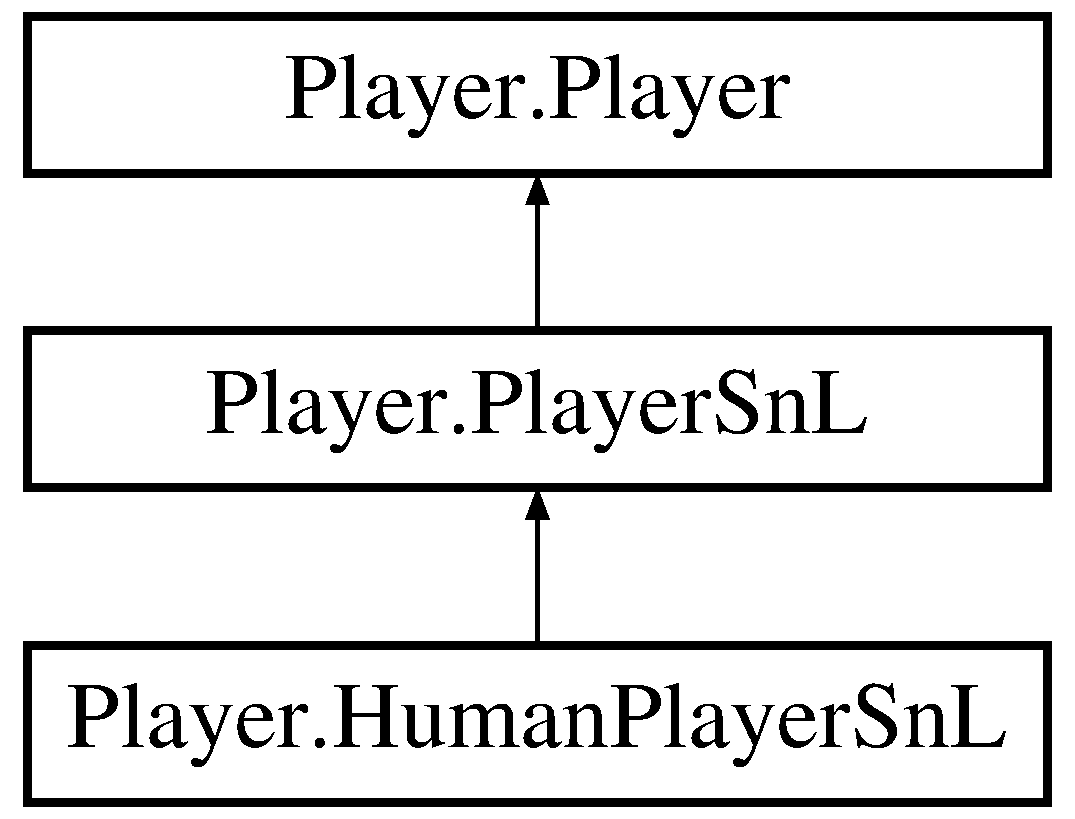
\includegraphics[height=3.000000cm]{class_player_1_1_human_player_sn_l}
\end{center}
\end{figure}
\subsection*{Public Member Functions}
\begin{DoxyCompactItemize}
\item 
\hyperlink{class_player_1_1_human_player_sn_l_a7605b134f337342fedb834ec55a03b7a}{Human\+Player\+Sn\+L} (String name, Color c)
\item 
\hyperlink{class_player_1_1_human_player_sn_l_ab22f9ceaee8c00bd22b6372d54452391}{Human\+Player\+Sn\+L} (String name, Color c, int position)
\end{DoxyCompactItemize}
\subsection*{Static Public Member Functions}
\begin{DoxyCompactItemize}
\item 
static void \hyperlink{class_player_1_1_human_player_sn_l_a74ccdaec9a1d4188bd8c6c79b2c7f712}{main} (String\mbox{[}$\,$\mbox{]} args)
\end{DoxyCompactItemize}
\subsection*{Additional Inherited Members}


\subsection{Detailed Description}
Creates a human player for Snake and Ladders. 

Definition at line 20 of file Human\+Player\+Sn\+L.\+java.



\subsection{Constructor \& Destructor Documentation}
\hypertarget{class_player_1_1_human_player_sn_l_a7605b134f337342fedb834ec55a03b7a}{}\index{Player\+::\+Human\+Player\+Sn\+L@{Player\+::\+Human\+Player\+Sn\+L}!Human\+Player\+Sn\+L@{Human\+Player\+Sn\+L}}
\index{Human\+Player\+Sn\+L@{Human\+Player\+Sn\+L}!Player\+::\+Human\+Player\+Sn\+L@{Player\+::\+Human\+Player\+Sn\+L}}
\subsubsection[{Human\+Player\+Sn\+L(\+String name, Color c)}]{\setlength{\rightskip}{0pt plus 5cm}Player.\+Human\+Player\+Sn\+L.\+Human\+Player\+Sn\+L (
\begin{DoxyParamCaption}
\item[{String}]{name, }
\item[{Color}]{c}
\end{DoxyParamCaption}
)}\label{class_player_1_1_human_player_sn_l_a7605b134f337342fedb834ec55a03b7a}
Constructor that save the player name and piece color to the class extends from \hyperlink{class_player_1_1_player}{Player} 
\begin{DoxyParams}{Parameters}
{\em name} & is the player name passed \\
\hline
{\em c} & is the player color passed \\
\hline
\end{DoxyParams}


Definition at line 29 of file Human\+Player\+Sn\+L.\+java.



References Menu.\+Game\+Selector.\+m\+\_\+\+T\+R\+A\+C\+E.



Referenced by Player.\+Human\+Player\+Sn\+L.\+main().

\hypertarget{class_player_1_1_human_player_sn_l_ab22f9ceaee8c00bd22b6372d54452391}{}\index{Player\+::\+Human\+Player\+Sn\+L@{Player\+::\+Human\+Player\+Sn\+L}!Human\+Player\+Sn\+L@{Human\+Player\+Sn\+L}}
\index{Human\+Player\+Sn\+L@{Human\+Player\+Sn\+L}!Player\+::\+Human\+Player\+Sn\+L@{Player\+::\+Human\+Player\+Sn\+L}}
\subsubsection[{Human\+Player\+Sn\+L(\+String name, Color c, int position)}]{\setlength{\rightskip}{0pt plus 5cm}Player.\+Human\+Player\+Sn\+L.\+Human\+Player\+Sn\+L (
\begin{DoxyParamCaption}
\item[{String}]{name, }
\item[{Color}]{c, }
\item[{int}]{position}
\end{DoxyParamCaption}
)}\label{class_player_1_1_human_player_sn_l_ab22f9ceaee8c00bd22b6372d54452391}
Constructor that save the player name and piece color and positions to the class extends from \hyperlink{class_player_1_1_player_sn_l}{Player\+Sn\+L} 
\begin{DoxyParams}{Parameters}
{\em name} & is the player name passed \\
\hline
{\em c} & is the player color passed \\
\hline
{\em position} & is the player current piece position \\
\hline
\end{DoxyParams}


Definition at line 46 of file Human\+Player\+Sn\+L.\+java.



References Menu.\+Game\+Selector.\+m\+\_\+\+T\+R\+A\+C\+E.



\subsection{Member Function Documentation}
\hypertarget{class_player_1_1_human_player_sn_l_a74ccdaec9a1d4188bd8c6c79b2c7f712}{}\index{Player\+::\+Human\+Player\+Sn\+L@{Player\+::\+Human\+Player\+Sn\+L}!main@{main}}
\index{main@{main}!Player\+::\+Human\+Player\+Sn\+L@{Player\+::\+Human\+Player\+Sn\+L}}
\subsubsection[{main(\+String[] args)}]{\setlength{\rightskip}{0pt plus 5cm}static void Player.\+Human\+Player\+Sn\+L.\+main (
\begin{DoxyParamCaption}
\item[{String   \mbox{[}$\,$\mbox{]}}]{args}
\end{DoxyParamCaption}
)\hspace{0.3cm}{\ttfamily [static]}}\label{class_player_1_1_human_player_sn_l_a74ccdaec9a1d4188bd8c6c79b2c7f712}
main method created for unit testing 
\begin{DoxyParams}{Parameters}
{\em args} & \\
\hline
\end{DoxyParams}


Definition at line 62 of file Human\+Player\+Sn\+L.\+java.



References Player.\+Human\+Player\+Sn\+L.\+Human\+Player\+Sn\+L().



The documentation for this class was generated from the following file\+:\begin{DoxyCompactItemize}
\item 
src/\+Player/\hyperlink{_human_player_sn_l_8java}{Human\+Player\+Sn\+L.\+java}\end{DoxyCompactItemize}

\hypertarget{class_player_1_1_human_player_t_t_t}{}\section{Player.\+Human\+Player\+T\+T\+T Class Reference}
\label{class_player_1_1_human_player_t_t_t}\index{Player.\+Human\+Player\+T\+T\+T@{Player.\+Human\+Player\+T\+T\+T}}


Creates a human player for Tic\+Tac\+Toe.  




Inheritance diagram for Player.\+Human\+Player\+T\+T\+T\+:\nopagebreak
\begin{figure}[H]
\begin{center}
\leavevmode
\includegraphics[width=204pt]{class_player_1_1_human_player_t_t_t__inherit__graph}
\end{center}
\end{figure}


Collaboration diagram for Player.\+Human\+Player\+T\+T\+T\+:\nopagebreak
\begin{figure}[H]
\begin{center}
\leavevmode
\includegraphics[width=283pt]{class_player_1_1_human_player_t_t_t__coll__graph}
\end{center}
\end{figure}
\subsection*{Public Member Functions}
\begin{DoxyCompactItemize}
\item 
\hyperlink{class_player_1_1_human_player_t_t_t_a617376ebf70bbb54f6ac722b1e9282a7}{Human\+Player\+T\+T\+T} (String name, char piece)
\item 
String \hyperlink{class_player_1_1_human_player_t_t_t_aadf14d433f944233d05f88cafb5e6a94}{get\+Player\+Name} ()
\item 
char \hyperlink{class_player_1_1_human_player_t_t_t_a3b80370f155683b77911850cc016e6a7}{get\+Player\+Piece\+Type} ()
\item 
boolean \hyperlink{class_player_1_1_human_player_t_t_t_a9c97f1c97829c9af212b8088e80ec7db}{is\+X} ()
\item 
boolean \hyperlink{class_player_1_1_human_player_t_t_t_acce1adf858320b165c07b8250b865edb}{is\+O} ()
\item 
int \hyperlink{class_player_1_1_human_player_t_t_t_a50f86fdac0e60ab7302f99f1ad25953b}{get\+Piece\+Location} ()
\item 
Array\+List$<$ Integer $>$ \hyperlink{class_player_1_1_human_player_t_t_t_accd55d5ba0f1bfc95ff64c3b15c57840}{get\+Piece\+Locations} ()
\item 
void \hyperlink{class_player_1_1_human_player_t_t_t_ab65859ad968e025536e8434efad24a6a}{add\+Piece} (\hyperlink{class_square_1_1_square}{Square} s)
\end{DoxyCompactItemize}
\subsection*{Static Public Member Functions}
\begin{DoxyCompactItemize}
\item 
static void \hyperlink{class_player_1_1_human_player_t_t_t_ae29df5ea96e348fdf342b47574e6b673}{main} (String\mbox{[}$\,$\mbox{]} args)
\end{DoxyCompactItemize}
\subsection*{Additional Inherited Members}


\subsection{Detailed Description}
Creates a human player for Tic\+Tac\+Toe. 

Definition at line 21 of file Human\+Player\+T\+T\+T.\+java.



\subsection{Constructor \& Destructor Documentation}
\hypertarget{class_player_1_1_human_player_t_t_t_a617376ebf70bbb54f6ac722b1e9282a7}{}\index{Player\+::\+Human\+Player\+T\+T\+T@{Player\+::\+Human\+Player\+T\+T\+T}!Human\+Player\+T\+T\+T@{Human\+Player\+T\+T\+T}}
\index{Human\+Player\+T\+T\+T@{Human\+Player\+T\+T\+T}!Player\+::\+Human\+Player\+T\+T\+T@{Player\+::\+Human\+Player\+T\+T\+T}}
\subsubsection[{Human\+Player\+T\+T\+T(\+String name, char piece)}]{\setlength{\rightskip}{0pt plus 5cm}Player.\+Human\+Player\+T\+T\+T.\+Human\+Player\+T\+T\+T (
\begin{DoxyParamCaption}
\item[{String}]{name, }
\item[{char}]{piece}
\end{DoxyParamCaption}
)}\label{class_player_1_1_human_player_t_t_t_a617376ebf70bbb54f6ac722b1e9282a7}
Constructor that save the human player name and piece to the class extends from \hyperlink{class_player_1_1_player_t_t_t}{Player\+T\+T\+T} 
\begin{DoxyParams}{Parameters}
{\em name} & is the player name passed \\
\hline
{\em piece} & is the player piece passed \\
\hline
\end{DoxyParams}


Definition at line 29 of file Human\+Player\+T\+T\+T.\+java.



References Menu.\+Game\+Selector.\+m\+\_\+\+T\+R\+A\+C\+E.



Referenced by Player.\+Human\+Player\+T\+T\+T.\+main().



\subsection{Member Function Documentation}
\hypertarget{class_player_1_1_human_player_t_t_t_ab65859ad968e025536e8434efad24a6a}{}\index{Player\+::\+Human\+Player\+T\+T\+T@{Player\+::\+Human\+Player\+T\+T\+T}!add\+Piece@{add\+Piece}}
\index{add\+Piece@{add\+Piece}!Player\+::\+Human\+Player\+T\+T\+T@{Player\+::\+Human\+Player\+T\+T\+T}}
\subsubsection[{add\+Piece(\+Square s)}]{\setlength{\rightskip}{0pt plus 5cm}void Player.\+Human\+Player\+T\+T\+T.\+add\+Piece (
\begin{DoxyParamCaption}
\item[{{\bf Square}}]{s}
\end{DoxyParamCaption}
)}\label{class_player_1_1_human_player_t_t_t_ab65859ad968e025536e8434efad24a6a}
Add Piece to Piece array extends from \hyperlink{class_player_1_1_player_t_t_t}{Player\+T\+T\+T} 
\begin{DoxyParams}{Parameters}
{\em s} & the square location you put the piece on \\
\hline
\end{DoxyParams}


Definition at line 126 of file Human\+Player\+T\+T\+T.\+java.



References Menu.\+Game\+Selector.\+m\+\_\+\+T\+R\+A\+C\+E.



Referenced by Player.\+Human\+Player\+T\+T\+T.\+main().

\hypertarget{class_player_1_1_human_player_t_t_t_a50f86fdac0e60ab7302f99f1ad25953b}{}\index{Player\+::\+Human\+Player\+T\+T\+T@{Player\+::\+Human\+Player\+T\+T\+T}!get\+Piece\+Location@{get\+Piece\+Location}}
\index{get\+Piece\+Location@{get\+Piece\+Location}!Player\+::\+Human\+Player\+T\+T\+T@{Player\+::\+Human\+Player\+T\+T\+T}}
\subsubsection[{get\+Piece\+Location()}]{\setlength{\rightskip}{0pt plus 5cm}int Player.\+Human\+Player\+T\+T\+T.\+get\+Piece\+Location (
\begin{DoxyParamCaption}
{}
\end{DoxyParamCaption}
)}\label{class_player_1_1_human_player_t_t_t_a50f86fdac0e60ab7302f99f1ad25953b}
Gets the player piece location extends from \hyperlink{class_player_1_1_player_t_t_t}{Player\+T\+T\+T} \begin{DoxyReturn}{Returns}
the player one piece location 
\end{DoxyReturn}


Definition at line 101 of file Human\+Player\+T\+T\+T.\+java.



References Menu.\+Game\+Selector.\+m\+\_\+\+T\+R\+A\+C\+E.



Referenced by Player.\+Human\+Player\+T\+T\+T.\+main().

\hypertarget{class_player_1_1_human_player_t_t_t_accd55d5ba0f1bfc95ff64c3b15c57840}{}\index{Player\+::\+Human\+Player\+T\+T\+T@{Player\+::\+Human\+Player\+T\+T\+T}!get\+Piece\+Locations@{get\+Piece\+Locations}}
\index{get\+Piece\+Locations@{get\+Piece\+Locations}!Player\+::\+Human\+Player\+T\+T\+T@{Player\+::\+Human\+Player\+T\+T\+T}}
\subsubsection[{get\+Piece\+Locations()}]{\setlength{\rightskip}{0pt plus 5cm}Array\+List$<$Integer$>$ Player.\+Human\+Player\+T\+T\+T.\+get\+Piece\+Locations (
\begin{DoxyParamCaption}
{}
\end{DoxyParamCaption}
)}\label{class_player_1_1_human_player_t_t_t_accd55d5ba0f1bfc95ff64c3b15c57840}
Gets the player piece location array extends from \hyperlink{class_player_1_1_player_t_t_t}{Player\+T\+T\+T} \begin{DoxyReturn}{Returns}
the player one piece location array 
\end{DoxyReturn}


Definition at line 113 of file Human\+Player\+T\+T\+T.\+java.



References Menu.\+Game\+Selector.\+m\+\_\+\+T\+R\+A\+C\+E.



Referenced by Player.\+Human\+Player\+T\+T\+T.\+main().

\hypertarget{class_player_1_1_human_player_t_t_t_aadf14d433f944233d05f88cafb5e6a94}{}\index{Player\+::\+Human\+Player\+T\+T\+T@{Player\+::\+Human\+Player\+T\+T\+T}!get\+Player\+Name@{get\+Player\+Name}}
\index{get\+Player\+Name@{get\+Player\+Name}!Player\+::\+Human\+Player\+T\+T\+T@{Player\+::\+Human\+Player\+T\+T\+T}}
\subsubsection[{get\+Player\+Name()}]{\setlength{\rightskip}{0pt plus 5cm}String Player.\+Human\+Player\+T\+T\+T.\+get\+Player\+Name (
\begin{DoxyParamCaption}
{}
\end{DoxyParamCaption}
)}\label{class_player_1_1_human_player_t_t_t_aadf14d433f944233d05f88cafb5e6a94}
Gets the player name \begin{DoxyReturn}{Returns}
the player name extends from \hyperlink{class_player_1_1_player}{Player} 
\end{DoxyReturn}


Definition at line 43 of file Human\+Player\+T\+T\+T.\+java.



References Menu.\+Game\+Selector.\+m\+\_\+\+T\+R\+A\+C\+E.



Referenced by Player.\+Human\+Player\+T\+T\+T.\+main().

\hypertarget{class_player_1_1_human_player_t_t_t_a3b80370f155683b77911850cc016e6a7}{}\index{Player\+::\+Human\+Player\+T\+T\+T@{Player\+::\+Human\+Player\+T\+T\+T}!get\+Player\+Piece\+Type@{get\+Player\+Piece\+Type}}
\index{get\+Player\+Piece\+Type@{get\+Player\+Piece\+Type}!Player\+::\+Human\+Player\+T\+T\+T@{Player\+::\+Human\+Player\+T\+T\+T}}
\subsubsection[{get\+Player\+Piece\+Type()}]{\setlength{\rightskip}{0pt plus 5cm}char Player.\+Human\+Player\+T\+T\+T.\+get\+Player\+Piece\+Type (
\begin{DoxyParamCaption}
{}
\end{DoxyParamCaption}
)}\label{class_player_1_1_human_player_t_t_t_a3b80370f155683b77911850cc016e6a7}
Gets the player piece type extends from player\+T\+T\+T \begin{DoxyReturn}{Returns}
the player piece type is X or O 
\end{DoxyReturn}


Definition at line 55 of file Human\+Player\+T\+T\+T.\+java.



References Menu.\+Game\+Selector.\+m\+\_\+\+T\+R\+A\+C\+E.



Referenced by Player.\+Human\+Player\+T\+T\+T.\+main().

\hypertarget{class_player_1_1_human_player_t_t_t_acce1adf858320b165c07b8250b865edb}{}\index{Player\+::\+Human\+Player\+T\+T\+T@{Player\+::\+Human\+Player\+T\+T\+T}!is\+O@{is\+O}}
\index{is\+O@{is\+O}!Player\+::\+Human\+Player\+T\+T\+T@{Player\+::\+Human\+Player\+T\+T\+T}}
\subsubsection[{is\+O()}]{\setlength{\rightskip}{0pt plus 5cm}boolean Player.\+Human\+Player\+T\+T\+T.\+is\+O (
\begin{DoxyParamCaption}
{}
\end{DoxyParamCaption}
)}\label{class_player_1_1_human_player_t_t_t_acce1adf858320b165c07b8250b865edb}
Check if the player piece is O or not \begin{DoxyReturn}{Returns}
the true if player\+Piece\+Type is O 
\end{DoxyReturn}


Definition at line 84 of file Human\+Player\+T\+T\+T.\+java.



References Menu.\+Game\+Selector.\+m\+\_\+\+T\+R\+A\+C\+E.



Referenced by Player.\+Human\+Player\+T\+T\+T.\+main().

\hypertarget{class_player_1_1_human_player_t_t_t_a9c97f1c97829c9af212b8088e80ec7db}{}\index{Player\+::\+Human\+Player\+T\+T\+T@{Player\+::\+Human\+Player\+T\+T\+T}!is\+X@{is\+X}}
\index{is\+X@{is\+X}!Player\+::\+Human\+Player\+T\+T\+T@{Player\+::\+Human\+Player\+T\+T\+T}}
\subsubsection[{is\+X()}]{\setlength{\rightskip}{0pt plus 5cm}boolean Player.\+Human\+Player\+T\+T\+T.\+is\+X (
\begin{DoxyParamCaption}
{}
\end{DoxyParamCaption}
)}\label{class_player_1_1_human_player_t_t_t_a9c97f1c97829c9af212b8088e80ec7db}
Check if the player piece is X or not \begin{DoxyReturn}{Returns}
the true if player\+Piece\+Type is X 
\end{DoxyReturn}


Definition at line 67 of file Human\+Player\+T\+T\+T.\+java.



References Menu.\+Game\+Selector.\+m\+\_\+\+T\+R\+A\+C\+E.



Referenced by Player.\+Human\+Player\+T\+T\+T.\+main().

\hypertarget{class_player_1_1_human_player_t_t_t_ae29df5ea96e348fdf342b47574e6b673}{}\index{Player\+::\+Human\+Player\+T\+T\+T@{Player\+::\+Human\+Player\+T\+T\+T}!main@{main}}
\index{main@{main}!Player\+::\+Human\+Player\+T\+T\+T@{Player\+::\+Human\+Player\+T\+T\+T}}
\subsubsection[{main(\+String[] args)}]{\setlength{\rightskip}{0pt plus 5cm}static void Player.\+Human\+Player\+T\+T\+T.\+main (
\begin{DoxyParamCaption}
\item[{String   \mbox{[}$\,$\mbox{]}}]{args}
\end{DoxyParamCaption}
)\hspace{0.3cm}{\ttfamily [static]}}\label{class_player_1_1_human_player_t_t_t_ae29df5ea96e348fdf342b47574e6b673}
main method created for unit testing 
\begin{DoxyParams}{Parameters}
{\em args} & \\
\hline
\end{DoxyParams}


Definition at line 139 of file Human\+Player\+T\+T\+T.\+java.



References Player.\+Human\+Player\+T\+T\+T.\+add\+Piece(), Player.\+Human\+Player\+T\+T\+T.\+get\+Piece\+Location(), Player.\+Human\+Player\+T\+T\+T.\+get\+Piece\+Locations(), Player.\+Human\+Player\+T\+T\+T.\+get\+Player\+Name(), Player.\+Human\+Player\+T\+T\+T.\+get\+Player\+Piece\+Type(), Player.\+Human\+Player\+T\+T\+T.\+Human\+Player\+T\+T\+T(), Player.\+Human\+Player\+T\+T\+T.\+is\+O(), and Player.\+Human\+Player\+T\+T\+T.\+is\+X().



The documentation for this class was generated from the following file\+:\begin{DoxyCompactItemize}
\item 
src/\+Player/\hyperlink{_human_player_t_t_t_8java}{Human\+Player\+T\+T\+T.\+java}\end{DoxyCompactItemize}

\hypertarget{class_menu_1_1_menu_sn_l}{}\section{Menu.\+Menu\+Sn\+L Class Reference}
\label{class_menu_1_1_menu_sn_l}\index{Menu.\+Menu\+Sn\+L@{Menu.\+Menu\+Sn\+L}}


The menu class specific to the Sn\+L game This class is for the menu of the Sn\+L game, covering the player colour selection, the number of players and the numbers of snakes and ladders on the board. The menu also allows for the input of player names.  


\subsection*{Public Member Functions}
\begin{DoxyCompactItemize}
\item 
\hyperlink{class_menu_1_1_menu_sn_l_a39167b25cf1ab4be1f66b6a327635e7b}{Menu\+Sn\+L} ()
\end{DoxyCompactItemize}
\subsection*{Static Public Member Functions}
\begin{DoxyCompactItemize}
\item 
static void \hyperlink{class_menu_1_1_menu_sn_l_af94b678ab820b841c5d39e683a7e26c5}{main} (String\mbox{[}$\,$\mbox{]} args)
\end{DoxyCompactItemize}
\subsection*{Private Member Functions}
\begin{DoxyCompactItemize}
\item 
void \hyperlink{class_menu_1_1_menu_sn_l_a66ee14babba3fc0a603c285f4e744581}{add\+Labels} ()
\item 
void \hyperlink{class_menu_1_1_menu_sn_l_a714ff7606c361986e72e620682b0cbed}{add\+Number\+Of\+Players\+Combo\+Box} ()
\item 
void \hyperlink{class_menu_1_1_menu_sn_l_a47dfa399fdd8326a8435d2df260a65e4}{add\+Players\+Names\+Text\+Field} ()
\item 
void \hyperlink{class_menu_1_1_menu_sn_l_a295ed859c68f12de97ebfb2626cefa73}{add\+Colours\+Combo\+Box} ()
\item 
void \hyperlink{class_menu_1_1_menu_sn_l_a4558c3f6394225f5d578fdef2b0bb6c2}{add\+Player\+Type} ()
\item 
void \hyperlink{class_menu_1_1_menu_sn_l_a76f7b84bc139f5a0ef501c9ffab9097e}{add\+Ladders\+Combo\+Box} ()
\item 
void \hyperlink{class_menu_1_1_menu_sn_l_a2cb25a2dd413640047630bdb601a72f3}{add\+Snakes\+Combo\+Box} ()
\item 
void \hyperlink{class_menu_1_1_menu_sn_l_ac2ef26c4da4cc4890cc11001265ff59b}{add\+Visualization\+Check\+Box} ()
\item 
void \hyperlink{class_menu_1_1_menu_sn_l_a3f156b20b897d2757d4b8bf6ff85495f}{add\+Logo} ()
\item 
void \hyperlink{class_menu_1_1_menu_sn_l_a1a36c2b37761e10a2c22918457820e6f}{add\+Game\+Buttons} ()
\item 
void \hyperlink{class_menu_1_1_menu_sn_l_aaee495e90ef87ac55c24fe65a460a676}{load\+Game} ()
\item 
void \hyperlink{class_menu_1_1_menu_sn_l_adf112a519d7f79a6b6d3ebf3f136d8aa}{send\+Form} ()
\end{DoxyCompactItemize}
\subsection*{Private Attributes}
\begin{DoxyCompactItemize}
\item 
final String \hyperlink{class_menu_1_1_menu_sn_l_a62bbb19bbedcdf63b575b4ae1048c343}{W\+I\+N\+D\+O\+W\+\_\+\+T\+I\+T\+L\+E} = \char`\"{}Snakes and Ladders\char`\"{}
\item 
final String\mbox{[}$\,$\mbox{]} \hyperlink{class_menu_1_1_menu_sn_l_accdb88464884a651bab3a9ebb5eb2beb}{S\+N\+L\+\_\+\+N\+U\+M\+B\+E\+R\+\_\+\+P\+L\+A\+Y\+E\+R\+S}
\item 
final String\mbox{[}$\,$\mbox{]} \hyperlink{class_menu_1_1_menu_sn_l_aa0aa3bcb48114b48faa0a49fa0c98504}{S\+N\+L\+\_\+\+C\+O\+L\+O\+R\+\_\+\+P\+L\+A\+Y\+E\+R\+S}
\item 
final String\mbox{[}$\,$\mbox{]} \hyperlink{class_menu_1_1_menu_sn_l_aa0ead71ad043fc5f187fde721b34c34b}{N\+U\+M\+B\+E\+R\+S\+\_\+\+O\+F\+\_\+\+O\+P\+T\+I\+O\+N\+S} = \{ \char`\"{}1\char`\"{}, \char`\"{}2\char`\"{}, \char`\"{}3\char`\"{}, \char`\"{}4\char`\"{} \}
\item 
final int \hyperlink{class_menu_1_1_menu_sn_l_a2fcacd6fe04ce3a540d0d100ca57b993}{W\+I\+N\+D\+O\+W\+\_\+\+W\+I\+D\+T\+H} = 500
\item 
final int \hyperlink{class_menu_1_1_menu_sn_l_a32c2e05c64b453df29d8b6df1061a939}{W\+I\+N\+D\+O\+W\+\_\+\+H\+E\+I\+G\+H\+T} = 550
\item 
final String\mbox{[}$\,$\mbox{]} \hyperlink{class_menu_1_1_menu_sn_l_a7cd650c1f3cf334aafb3be5b3ad1b158}{H\+U\+M\+A\+N\+\_\+\+O\+R\+\_\+\+A\+I} = \{\char`\"{}Human\char`\"{}, \char`\"{}A\+I\char`\"{}\}
\item 
final int \hyperlink{class_menu_1_1_menu_sn_l_afc7fd19db34602b6b5a85df60c736103}{M\+A\+X\+\_\+\+N\+U\+M\+\_\+\+P\+L\+A\+Y\+E\+R\+S} = 4
\item 
J\+Frame \hyperlink{class_menu_1_1_menu_sn_l_af43a9353bb0cfe3d29fa37d67b794a65}{m\+\_\+frame}
\item 
Array\+List$<$ J\+Text\+Field $>$ \hyperlink{class_menu_1_1_menu_sn_l_a8e5b5896ffe07afef10443fe99b45dab}{m\+\_\+players\+Name\+Text\+Field}
\item 
Array\+List$<$ J\+Combo\+Box$<$ String $>$ $>$ \hyperlink{class_menu_1_1_menu_sn_l_a99b5b387a1ff9257d77534ebff7ca370}{m\+\_\+players\+Colours}
\item 
Array\+List$<$ J\+Label $>$ \hyperlink{class_menu_1_1_menu_sn_l_ab29efffc6315a328efb34fed209c0677}{m\+\_\+name\+Players\+Label}
\item 
Array\+List$<$ J\+Combo\+Box$<$ String $>$ $>$ \hyperlink{class_menu_1_1_menu_sn_l_a70c6fa4562124ab11bab5d572daf82b3}{m\+\_\+player\+Type\+Combo\+Box}
\item 
J\+Button \hyperlink{class_menu_1_1_menu_sn_l_ac45af15bf2aabd1916063700e1e44f08}{m\+\_\+init\+Game\+Button}
\item 
J\+Combo\+Box$<$ String $>$ \hyperlink{class_menu_1_1_menu_sn_l_a52b5fdac24b1860a453eee6f505208da}{m\+\_\+players\+Combo\+Box}
\item 
int \hyperlink{class_menu_1_1_menu_sn_l_afee3307aa062adfbee4edd14484c8f2c}{m\+\_\+number\+Players} = 0
\item 
J\+Combo\+Box$<$ String $>$ \hyperlink{class_menu_1_1_menu_sn_l_acc735c8e538c308d888618f726ddd344}{m\+\_\+player\+Snakes}
\item 
J\+Combo\+Box$<$ String $>$ \hyperlink{class_menu_1_1_menu_sn_l_a75cae58abbeef1dc893ab2214f84aaad}{m\+\_\+player\+Ladders}
\item 
int \hyperlink{class_menu_1_1_menu_sn_l_a5787c03e612eb9adb0f0ee976810be88}{m\+\_\+snakes\+No} = 1
\item 
int \hyperlink{class_menu_1_1_menu_sn_l_a30c87e65118ddf61c75fa3d9d9abe36e}{m\+\_\+ladders\+No} = 1
\item 
J\+Check\+Box \hyperlink{class_menu_1_1_menu_sn_l_a774bdc16dab9d1c0c882d2212beb70ac}{visualization}
\end{DoxyCompactItemize}


\subsection{Detailed Description}
The menu class specific to the Sn\+L game This class is for the menu of the Sn\+L game, covering the player colour selection, the number of players and the numbers of snakes and ladders on the board. The menu also allows for the input of player names. 

Definition at line 49 of file Menu\+Sn\+L.\+java.



\subsection{Constructor \& Destructor Documentation}
\hypertarget{class_menu_1_1_menu_sn_l_a39167b25cf1ab4be1f66b6a327635e7b}{}\index{Menu\+::\+Menu\+Sn\+L@{Menu\+::\+Menu\+Sn\+L}!Menu\+Sn\+L@{Menu\+Sn\+L}}
\index{Menu\+Sn\+L@{Menu\+Sn\+L}!Menu\+::\+Menu\+Sn\+L@{Menu\+::\+Menu\+Sn\+L}}
\subsubsection[{Menu\+Sn\+L()}]{\setlength{\rightskip}{0pt plus 5cm}Menu.\+Menu\+Sn\+L.\+Menu\+Sn\+L (
\begin{DoxyParamCaption}
{}
\end{DoxyParamCaption}
)}\label{class_menu_1_1_menu_sn_l_a39167b25cf1ab4be1f66b6a327635e7b}
This is the \hyperlink{class_menu_1_1_menu_sn_l}{Menu\+Sn\+L} constructor. It sets up a new frame setting its height and width. 

Definition at line 145 of file Menu\+Sn\+L.\+java.



References Menu.\+Menu\+Sn\+L.\+add\+Colours\+Combo\+Box(), Menu.\+Menu\+Sn\+L.\+add\+Game\+Buttons(), Menu.\+Menu\+Sn\+L.\+add\+Labels(), Menu.\+Menu\+Sn\+L.\+add\+Ladders\+Combo\+Box(), Menu.\+Menu\+Sn\+L.\+add\+Logo(), Menu.\+Menu\+Sn\+L.\+add\+Number\+Of\+Players\+Combo\+Box(), Menu.\+Menu\+Sn\+L.\+add\+Players\+Names\+Text\+Field(), Menu.\+Menu\+Sn\+L.\+add\+Player\+Type(), Menu.\+Menu\+Sn\+L.\+add\+Snakes\+Combo\+Box(), Menu.\+Menu\+Sn\+L.\+add\+Visualization\+Check\+Box(), and Menu.\+Game\+Selector.\+m\+\_\+\+T\+R\+A\+C\+E.



Referenced by Menu.\+Menu\+Sn\+L.\+main().



\subsection{Member Function Documentation}
\hypertarget{class_menu_1_1_menu_sn_l_a295ed859c68f12de97ebfb2626cefa73}{}\index{Menu\+::\+Menu\+Sn\+L@{Menu\+::\+Menu\+Sn\+L}!add\+Colours\+Combo\+Box@{add\+Colours\+Combo\+Box}}
\index{add\+Colours\+Combo\+Box@{add\+Colours\+Combo\+Box}!Menu\+::\+Menu\+Sn\+L@{Menu\+::\+Menu\+Sn\+L}}
\subsubsection[{add\+Colours\+Combo\+Box()}]{\setlength{\rightskip}{0pt plus 5cm}void Menu.\+Menu\+Sn\+L.\+add\+Colours\+Combo\+Box (
\begin{DoxyParamCaption}
{}
\end{DoxyParamCaption}
)\hspace{0.3cm}{\ttfamily [private]}}\label{class_menu_1_1_menu_sn_l_a295ed859c68f12de97ebfb2626cefa73}
Adds the combo box to the screen to select the player\textquotesingle{}s colours. 

Definition at line 281 of file Menu\+Sn\+L.\+java.



References Menu.\+Game\+Selector.\+m\+\_\+\+T\+R\+A\+C\+E, and Menu.\+Menu\+Sn\+L.\+M\+A\+X\+\_\+\+N\+U\+M\+\_\+\+P\+L\+A\+Y\+E\+R\+S.



Referenced by Menu.\+Menu\+Sn\+L.\+main(), and Menu.\+Menu\+Sn\+L.\+Menu\+Sn\+L().

\hypertarget{class_menu_1_1_menu_sn_l_a1a36c2b37761e10a2c22918457820e6f}{}\index{Menu\+::\+Menu\+Sn\+L@{Menu\+::\+Menu\+Sn\+L}!add\+Game\+Buttons@{add\+Game\+Buttons}}
\index{add\+Game\+Buttons@{add\+Game\+Buttons}!Menu\+::\+Menu\+Sn\+L@{Menu\+::\+Menu\+Sn\+L}}
\subsubsection[{add\+Game\+Buttons()}]{\setlength{\rightskip}{0pt plus 5cm}void Menu.\+Menu\+Sn\+L.\+add\+Game\+Buttons (
\begin{DoxyParamCaption}
{}
\end{DoxyParamCaption}
)\hspace{0.3cm}{\ttfamily [private]}}\label{class_menu_1_1_menu_sn_l_a1a36c2b37761e10a2c22918457820e6f}
Adds the start, load and back button to the frame. 

Definition at line 405 of file Menu\+Sn\+L.\+java.



References Menu.\+Menu\+Sn\+L.\+load\+Game(), Menu.\+Game\+Selector.\+m\+\_\+\+T\+R\+A\+C\+E, and Menu.\+Menu\+Sn\+L.\+send\+Form().



Referenced by Menu.\+Menu\+Sn\+L.\+main(), and Menu.\+Menu\+Sn\+L.\+Menu\+Sn\+L().

\hypertarget{class_menu_1_1_menu_sn_l_a66ee14babba3fc0a603c285f4e744581}{}\index{Menu\+::\+Menu\+Sn\+L@{Menu\+::\+Menu\+Sn\+L}!add\+Labels@{add\+Labels}}
\index{add\+Labels@{add\+Labels}!Menu\+::\+Menu\+Sn\+L@{Menu\+::\+Menu\+Sn\+L}}
\subsubsection[{add\+Labels()}]{\setlength{\rightskip}{0pt plus 5cm}void Menu.\+Menu\+Sn\+L.\+add\+Labels (
\begin{DoxyParamCaption}
{}
\end{DoxyParamCaption}
)\hspace{0.3cm}{\ttfamily [private]}}\label{class_menu_1_1_menu_sn_l_a66ee14babba3fc0a603c285f4e744581}
Adds the labels on the frame for the title, number of players, number of snakes, number of ladders. 

Definition at line 177 of file Menu\+Sn\+L.\+java.



References Menu.\+Game\+Selector.\+m\+\_\+\+T\+R\+A\+C\+E, and Menu.\+Menu\+Sn\+L.\+M\+A\+X\+\_\+\+N\+U\+M\+\_\+\+P\+L\+A\+Y\+E\+R\+S.



Referenced by Menu.\+Menu\+Sn\+L.\+main(), and Menu.\+Menu\+Sn\+L.\+Menu\+Sn\+L().

\hypertarget{class_menu_1_1_menu_sn_l_a76f7b84bc139f5a0ef501c9ffab9097e}{}\index{Menu\+::\+Menu\+Sn\+L@{Menu\+::\+Menu\+Sn\+L}!add\+Ladders\+Combo\+Box@{add\+Ladders\+Combo\+Box}}
\index{add\+Ladders\+Combo\+Box@{add\+Ladders\+Combo\+Box}!Menu\+::\+Menu\+Sn\+L@{Menu\+::\+Menu\+Sn\+L}}
\subsubsection[{add\+Ladders\+Combo\+Box()}]{\setlength{\rightskip}{0pt plus 5cm}void Menu.\+Menu\+Sn\+L.\+add\+Ladders\+Combo\+Box (
\begin{DoxyParamCaption}
{}
\end{DoxyParamCaption}
)\hspace{0.3cm}{\ttfamily [private]}}\label{class_menu_1_1_menu_sn_l_a76f7b84bc139f5a0ef501c9ffab9097e}
Adds the combo box to the frame to select the number of ladders. 

Definition at line 320 of file Menu\+Sn\+L.\+java.



References Menu.\+Game\+Selector.\+m\+\_\+\+T\+R\+A\+C\+E, and Menu.\+Menu\+Sn\+L.\+N\+U\+M\+B\+E\+R\+S\+\_\+\+O\+F\+\_\+\+O\+P\+T\+I\+O\+N\+S.



Referenced by Menu.\+Menu\+Sn\+L.\+main(), and Menu.\+Menu\+Sn\+L.\+Menu\+Sn\+L().

\hypertarget{class_menu_1_1_menu_sn_l_a3f156b20b897d2757d4b8bf6ff85495f}{}\index{Menu\+::\+Menu\+Sn\+L@{Menu\+::\+Menu\+Sn\+L}!add\+Logo@{add\+Logo}}
\index{add\+Logo@{add\+Logo}!Menu\+::\+Menu\+Sn\+L@{Menu\+::\+Menu\+Sn\+L}}
\subsubsection[{add\+Logo()}]{\setlength{\rightskip}{0pt plus 5cm}void Menu.\+Menu\+Sn\+L.\+add\+Logo (
\begin{DoxyParamCaption}
{}
\end{DoxyParamCaption}
)\hspace{0.3cm}{\ttfamily [private]}}\label{class_menu_1_1_menu_sn_l_a3f156b20b897d2757d4b8bf6ff85495f}
Adds the snakes and ladders logo to the frame. 

Definition at line 389 of file Menu\+Sn\+L.\+java.



References Menu.\+Game\+Selector.\+m\+\_\+\+T\+R\+A\+C\+E.



Referenced by Menu.\+Menu\+Sn\+L.\+main(), and Menu.\+Menu\+Sn\+L.\+Menu\+Sn\+L().

\hypertarget{class_menu_1_1_menu_sn_l_a714ff7606c361986e72e620682b0cbed}{}\index{Menu\+::\+Menu\+Sn\+L@{Menu\+::\+Menu\+Sn\+L}!add\+Number\+Of\+Players\+Combo\+Box@{add\+Number\+Of\+Players\+Combo\+Box}}
\index{add\+Number\+Of\+Players\+Combo\+Box@{add\+Number\+Of\+Players\+Combo\+Box}!Menu\+::\+Menu\+Sn\+L@{Menu\+::\+Menu\+Sn\+L}}
\subsubsection[{add\+Number\+Of\+Players\+Combo\+Box()}]{\setlength{\rightskip}{0pt plus 5cm}void Menu.\+Menu\+Sn\+L.\+add\+Number\+Of\+Players\+Combo\+Box (
\begin{DoxyParamCaption}
{}
\end{DoxyParamCaption}
)\hspace{0.3cm}{\ttfamily [private]}}\label{class_menu_1_1_menu_sn_l_a714ff7606c361986e72e620682b0cbed}
Creates a combo box to select the number of players. 

Definition at line 217 of file Menu\+Sn\+L.\+java.



References Menu.\+Menu\+Sn\+L.\+m\+\_\+number\+Players, Menu.\+Game\+Selector.\+m\+\_\+\+T\+R\+A\+C\+E, Menu.\+Menu\+Sn\+L.\+M\+A\+X\+\_\+\+N\+U\+M\+\_\+\+P\+L\+A\+Y\+E\+R\+S, and Menu.\+Menu\+Sn\+L.\+S\+N\+L\+\_\+\+N\+U\+M\+B\+E\+R\+\_\+\+P\+L\+A\+Y\+E\+R\+S.



Referenced by Menu.\+Menu\+Sn\+L.\+main(), and Menu.\+Menu\+Sn\+L.\+Menu\+Sn\+L().

\hypertarget{class_menu_1_1_menu_sn_l_a47dfa399fdd8326a8435d2df260a65e4}{}\index{Menu\+::\+Menu\+Sn\+L@{Menu\+::\+Menu\+Sn\+L}!add\+Players\+Names\+Text\+Field@{add\+Players\+Names\+Text\+Field}}
\index{add\+Players\+Names\+Text\+Field@{add\+Players\+Names\+Text\+Field}!Menu\+::\+Menu\+Sn\+L@{Menu\+::\+Menu\+Sn\+L}}
\subsubsection[{add\+Players\+Names\+Text\+Field()}]{\setlength{\rightskip}{0pt plus 5cm}void Menu.\+Menu\+Sn\+L.\+add\+Players\+Names\+Text\+Field (
\begin{DoxyParamCaption}
{}
\end{DoxyParamCaption}
)\hspace{0.3cm}{\ttfamily [private]}}\label{class_menu_1_1_menu_sn_l_a47dfa399fdd8326a8435d2df260a65e4}
Adds the text fields to the frame to set the player\textquotesingle{}s names. 

Definition at line 265 of file Menu\+Sn\+L.\+java.



References Menu.\+Game\+Selector.\+m\+\_\+\+T\+R\+A\+C\+E, and Menu.\+Menu\+Sn\+L.\+M\+A\+X\+\_\+\+N\+U\+M\+\_\+\+P\+L\+A\+Y\+E\+R\+S.



Referenced by Menu.\+Menu\+Sn\+L.\+main(), and Menu.\+Menu\+Sn\+L.\+Menu\+Sn\+L().

\hypertarget{class_menu_1_1_menu_sn_l_a4558c3f6394225f5d578fdef2b0bb6c2}{}\index{Menu\+::\+Menu\+Sn\+L@{Menu\+::\+Menu\+Sn\+L}!add\+Player\+Type@{add\+Player\+Type}}
\index{add\+Player\+Type@{add\+Player\+Type}!Menu\+::\+Menu\+Sn\+L@{Menu\+::\+Menu\+Sn\+L}}
\subsubsection[{add\+Player\+Type()}]{\setlength{\rightskip}{0pt plus 5cm}void Menu.\+Menu\+Sn\+L.\+add\+Player\+Type (
\begin{DoxyParamCaption}
{}
\end{DoxyParamCaption}
)\hspace{0.3cm}{\ttfamily [private]}}\label{class_menu_1_1_menu_sn_l_a4558c3f6394225f5d578fdef2b0bb6c2}
Adds the combo box to set the player type 

Definition at line 304 of file Menu\+Sn\+L.\+java.



References Menu.\+Game\+Selector.\+m\+\_\+\+T\+R\+A\+C\+E, and Menu.\+Menu\+Sn\+L.\+M\+A\+X\+\_\+\+N\+U\+M\+\_\+\+P\+L\+A\+Y\+E\+R\+S.



Referenced by Menu.\+Menu\+Sn\+L.\+main(), and Menu.\+Menu\+Sn\+L.\+Menu\+Sn\+L().

\hypertarget{class_menu_1_1_menu_sn_l_a2cb25a2dd413640047630bdb601a72f3}{}\index{Menu\+::\+Menu\+Sn\+L@{Menu\+::\+Menu\+Sn\+L}!add\+Snakes\+Combo\+Box@{add\+Snakes\+Combo\+Box}}
\index{add\+Snakes\+Combo\+Box@{add\+Snakes\+Combo\+Box}!Menu\+::\+Menu\+Sn\+L@{Menu\+::\+Menu\+Sn\+L}}
\subsubsection[{add\+Snakes\+Combo\+Box()}]{\setlength{\rightskip}{0pt plus 5cm}void Menu.\+Menu\+Sn\+L.\+add\+Snakes\+Combo\+Box (
\begin{DoxyParamCaption}
{}
\end{DoxyParamCaption}
)\hspace{0.3cm}{\ttfamily [private]}}\label{class_menu_1_1_menu_sn_l_a2cb25a2dd413640047630bdb601a72f3}
Adds the combo box to the frame to select the number of ladders. 

Definition at line 340 of file Menu\+Sn\+L.\+java.



References Menu.\+Game\+Selector.\+m\+\_\+\+T\+R\+A\+C\+E, and Menu.\+Menu\+Sn\+L.\+N\+U\+M\+B\+E\+R\+S\+\_\+\+O\+F\+\_\+\+O\+P\+T\+I\+O\+N\+S.



Referenced by Menu.\+Menu\+Sn\+L.\+main(), and Menu.\+Menu\+Sn\+L.\+Menu\+Sn\+L().

\hypertarget{class_menu_1_1_menu_sn_l_ac2ef26c4da4cc4890cc11001265ff59b}{}\index{Menu\+::\+Menu\+Sn\+L@{Menu\+::\+Menu\+Sn\+L}!add\+Visualization\+Check\+Box@{add\+Visualization\+Check\+Box}}
\index{add\+Visualization\+Check\+Box@{add\+Visualization\+Check\+Box}!Menu\+::\+Menu\+Sn\+L@{Menu\+::\+Menu\+Sn\+L}}
\subsubsection[{add\+Visualization\+Check\+Box()}]{\setlength{\rightskip}{0pt plus 5cm}void Menu.\+Menu\+Sn\+L.\+add\+Visualization\+Check\+Box (
\begin{DoxyParamCaption}
{}
\end{DoxyParamCaption}
)\hspace{0.3cm}{\ttfamily [private]}}\label{class_menu_1_1_menu_sn_l_ac2ef26c4da4cc4890cc11001265ff59b}
Adds the visualization check box to the frame. 

Definition at line 360 of file Menu\+Sn\+L.\+java.



References Menu.\+Game\+Selector.\+m\+\_\+\+T\+R\+A\+C\+E.



Referenced by Menu.\+Menu\+Sn\+L.\+Menu\+Sn\+L().

\hypertarget{class_menu_1_1_menu_sn_l_aaee495e90ef87ac55c24fe65a460a676}{}\index{Menu\+::\+Menu\+Sn\+L@{Menu\+::\+Menu\+Sn\+L}!load\+Game@{load\+Game}}
\index{load\+Game@{load\+Game}!Menu\+::\+Menu\+Sn\+L@{Menu\+::\+Menu\+Sn\+L}}
\subsubsection[{load\+Game()}]{\setlength{\rightskip}{0pt plus 5cm}void Menu.\+Menu\+Sn\+L.\+load\+Game (
\begin{DoxyParamCaption}
{}
\end{DoxyParamCaption}
)\hspace{0.3cm}{\ttfamily [private]}}\label{class_menu_1_1_menu_sn_l_aaee495e90ef87ac55c24fe65a460a676}
loads the game from the file res/save\+Sn\+L 

Definition at line 460 of file Menu\+Sn\+L.\+java.



References Menu.\+Game\+Selector.\+m\+\_\+\+T\+R\+A\+C\+E.



Referenced by Menu.\+Menu\+Sn\+L.\+add\+Game\+Buttons(), and Menu.\+Menu\+Sn\+L.\+main().

\hypertarget{class_menu_1_1_menu_sn_l_af94b678ab820b841c5d39e683a7e26c5}{}\index{Menu\+::\+Menu\+Sn\+L@{Menu\+::\+Menu\+Sn\+L}!main@{main}}
\index{main@{main}!Menu\+::\+Menu\+Sn\+L@{Menu\+::\+Menu\+Sn\+L}}
\subsubsection[{main(\+String[] args)}]{\setlength{\rightskip}{0pt plus 5cm}static void Menu.\+Menu\+Sn\+L.\+main (
\begin{DoxyParamCaption}
\item[{String\mbox{[}$\,$\mbox{]}}]{args}
\end{DoxyParamCaption}
)\hspace{0.3cm}{\ttfamily [static]}}\label{class_menu_1_1_menu_sn_l_af94b678ab820b841c5d39e683a7e26c5}
This is the test method. It calls the menu\+Sn\+L constructor to add all the correct buttons, all methods are voids so it\textquotesingle{}s impossible to input invalid information. All methods are called, if no load game file available it will try to start the game with no player information throwing an error. 

Definition at line 126 of file Menu\+Sn\+L.\+java.



References Menu.\+Menu\+Sn\+L.\+add\+Colours\+Combo\+Box(), Menu.\+Menu\+Sn\+L.\+add\+Game\+Buttons(), Menu.\+Menu\+Sn\+L.\+add\+Labels(), Menu.\+Menu\+Sn\+L.\+add\+Ladders\+Combo\+Box(), Menu.\+Menu\+Sn\+L.\+add\+Logo(), Menu.\+Menu\+Sn\+L.\+add\+Number\+Of\+Players\+Combo\+Box(), Menu.\+Menu\+Sn\+L.\+add\+Players\+Names\+Text\+Field(), Menu.\+Menu\+Sn\+L.\+add\+Player\+Type(), Menu.\+Menu\+Sn\+L.\+add\+Snakes\+Combo\+Box(), Menu.\+Menu\+Sn\+L.\+load\+Game(), Menu.\+Menu\+Sn\+L.\+Menu\+Sn\+L(), and Menu.\+Menu\+Sn\+L.\+send\+Form().

\hypertarget{class_menu_1_1_menu_sn_l_adf112a519d7f79a6b6d3ebf3f136d8aa}{}\index{Menu\+::\+Menu\+Sn\+L@{Menu\+::\+Menu\+Sn\+L}!send\+Form@{send\+Form}}
\index{send\+Form@{send\+Form}!Menu\+::\+Menu\+Sn\+L@{Menu\+::\+Menu\+Sn\+L}}
\subsubsection[{send\+Form()}]{\setlength{\rightskip}{0pt plus 5cm}void Menu.\+Menu\+Sn\+L.\+send\+Form (
\begin{DoxyParamCaption}
{}
\end{DoxyParamCaption}
)\hspace{0.3cm}{\ttfamily [private]}}\label{class_menu_1_1_menu_sn_l_adf112a519d7f79a6b6d3ebf3f136d8aa}
Sends the information of all the players and the number of snakes and ladders to Game\+Snl. 

Definition at line 561 of file Menu\+Sn\+L.\+java.



References Menu.\+Menu\+Sn\+L.\+m\+\_\+number\+Players, and Menu.\+Game\+Selector.\+m\+\_\+\+T\+R\+A\+C\+E.



Referenced by Menu.\+Menu\+Sn\+L.\+add\+Game\+Buttons(), and Menu.\+Menu\+Sn\+L.\+main().



\subsection{Member Data Documentation}
\hypertarget{class_menu_1_1_menu_sn_l_a7cd650c1f3cf334aafb3be5b3ad1b158}{}\index{Menu\+::\+Menu\+Sn\+L@{Menu\+::\+Menu\+Sn\+L}!H\+U\+M\+A\+N\+\_\+\+O\+R\+\_\+\+A\+I@{H\+U\+M\+A\+N\+\_\+\+O\+R\+\_\+\+A\+I}}
\index{H\+U\+M\+A\+N\+\_\+\+O\+R\+\_\+\+A\+I@{H\+U\+M\+A\+N\+\_\+\+O\+R\+\_\+\+A\+I}!Menu\+::\+Menu\+Sn\+L@{Menu\+::\+Menu\+Sn\+L}}
\subsubsection[{H\+U\+M\+A\+N\+\_\+\+O\+R\+\_\+\+A\+I}]{\setlength{\rightskip}{0pt plus 5cm}final String \mbox{[}$\,$\mbox{]} Menu.\+Menu\+Sn\+L.\+H\+U\+M\+A\+N\+\_\+\+O\+R\+\_\+\+A\+I = \{\char`\"{}Human\char`\"{}, \char`\"{}A\+I\char`\"{}\}\hspace{0.3cm}{\ttfamily [private]}}\label{class_menu_1_1_menu_sn_l_a7cd650c1f3cf334aafb3be5b3ad1b158}
Array to hold the type of players 

Definition at line 73 of file Menu\+Sn\+L.\+java.

\hypertarget{class_menu_1_1_menu_sn_l_af43a9353bb0cfe3d29fa37d67b794a65}{}\index{Menu\+::\+Menu\+Sn\+L@{Menu\+::\+Menu\+Sn\+L}!m\+\_\+frame@{m\+\_\+frame}}
\index{m\+\_\+frame@{m\+\_\+frame}!Menu\+::\+Menu\+Sn\+L@{Menu\+::\+Menu\+Sn\+L}}
\subsubsection[{m\+\_\+frame}]{\setlength{\rightskip}{0pt plus 5cm}J\+Frame Menu.\+Menu\+Sn\+L.\+m\+\_\+frame\hspace{0.3cm}{\ttfamily [private]}}\label{class_menu_1_1_menu_sn_l_af43a9353bb0cfe3d29fa37d67b794a65}
Frame for the Snakes and Ladders \hyperlink{namespace_menu}{Menu} 

Definition at line 81 of file Menu\+Sn\+L.\+java.

\hypertarget{class_menu_1_1_menu_sn_l_ac45af15bf2aabd1916063700e1e44f08}{}\index{Menu\+::\+Menu\+Sn\+L@{Menu\+::\+Menu\+Sn\+L}!m\+\_\+init\+Game\+Button@{m\+\_\+init\+Game\+Button}}
\index{m\+\_\+init\+Game\+Button@{m\+\_\+init\+Game\+Button}!Menu\+::\+Menu\+Sn\+L@{Menu\+::\+Menu\+Sn\+L}}
\subsubsection[{m\+\_\+init\+Game\+Button}]{\setlength{\rightskip}{0pt plus 5cm}J\+Button Menu.\+Menu\+Sn\+L.\+m\+\_\+init\+Game\+Button\hspace{0.3cm}{\ttfamily [private]}}\label{class_menu_1_1_menu_sn_l_ac45af15bf2aabd1916063700e1e44f08}
Button to start game 

Definition at line 96 of file Menu\+Sn\+L.\+java.

\hypertarget{class_menu_1_1_menu_sn_l_a30c87e65118ddf61c75fa3d9d9abe36e}{}\index{Menu\+::\+Menu\+Sn\+L@{Menu\+::\+Menu\+Sn\+L}!m\+\_\+ladders\+No@{m\+\_\+ladders\+No}}
\index{m\+\_\+ladders\+No@{m\+\_\+ladders\+No}!Menu\+::\+Menu\+Sn\+L@{Menu\+::\+Menu\+Sn\+L}}
\subsubsection[{m\+\_\+ladders\+No}]{\setlength{\rightskip}{0pt plus 5cm}int Menu.\+Menu\+Sn\+L.\+m\+\_\+ladders\+No = 1\hspace{0.3cm}{\ttfamily [private]}}\label{class_menu_1_1_menu_sn_l_a30c87e65118ddf61c75fa3d9d9abe36e}
Number of ladders initialised to 1 

Definition at line 114 of file Menu\+Sn\+L.\+java.

\hypertarget{class_menu_1_1_menu_sn_l_ab29efffc6315a328efb34fed209c0677}{}\index{Menu\+::\+Menu\+Sn\+L@{Menu\+::\+Menu\+Sn\+L}!m\+\_\+name\+Players\+Label@{m\+\_\+name\+Players\+Label}}
\index{m\+\_\+name\+Players\+Label@{m\+\_\+name\+Players\+Label}!Menu\+::\+Menu\+Sn\+L@{Menu\+::\+Menu\+Sn\+L}}
\subsubsection[{m\+\_\+name\+Players\+Label}]{\setlength{\rightskip}{0pt plus 5cm}Array\+List$<$J\+Label$>$ Menu.\+Menu\+Sn\+L.\+m\+\_\+name\+Players\+Label\hspace{0.3cm}{\ttfamily [private]}}\label{class_menu_1_1_menu_sn_l_ab29efffc6315a328efb34fed209c0677}
Array list of player name label 

Definition at line 90 of file Menu\+Sn\+L.\+java.

\hypertarget{class_menu_1_1_menu_sn_l_afee3307aa062adfbee4edd14484c8f2c}{}\index{Menu\+::\+Menu\+Sn\+L@{Menu\+::\+Menu\+Sn\+L}!m\+\_\+number\+Players@{m\+\_\+number\+Players}}
\index{m\+\_\+number\+Players@{m\+\_\+number\+Players}!Menu\+::\+Menu\+Sn\+L@{Menu\+::\+Menu\+Sn\+L}}
\subsubsection[{m\+\_\+number\+Players}]{\setlength{\rightskip}{0pt plus 5cm}int Menu.\+Menu\+Sn\+L.\+m\+\_\+number\+Players = 0\hspace{0.3cm}{\ttfamily [private]}}\label{class_menu_1_1_menu_sn_l_afee3307aa062adfbee4edd14484c8f2c}
Number of players, initialised to 0 

Definition at line 102 of file Menu\+Sn\+L.\+java.



Referenced by Menu.\+Menu\+Sn\+L.\+add\+Number\+Of\+Players\+Combo\+Box(), and Menu.\+Menu\+Sn\+L.\+send\+Form().

\hypertarget{class_menu_1_1_menu_sn_l_a75cae58abbeef1dc893ab2214f84aaad}{}\index{Menu\+::\+Menu\+Sn\+L@{Menu\+::\+Menu\+Sn\+L}!m\+\_\+player\+Ladders@{m\+\_\+player\+Ladders}}
\index{m\+\_\+player\+Ladders@{m\+\_\+player\+Ladders}!Menu\+::\+Menu\+Sn\+L@{Menu\+::\+Menu\+Sn\+L}}
\subsubsection[{m\+\_\+player\+Ladders}]{\setlength{\rightskip}{0pt plus 5cm}J\+Combo\+Box$<$String$>$ Menu.\+Menu\+Sn\+L.\+m\+\_\+player\+Ladders\hspace{0.3cm}{\ttfamily [private]}}\label{class_menu_1_1_menu_sn_l_a75cae58abbeef1dc893ab2214f84aaad}
Combo box to select number of ladders 

Definition at line 108 of file Menu\+Sn\+L.\+java.

\hypertarget{class_menu_1_1_menu_sn_l_a99b5b387a1ff9257d77534ebff7ca370}{}\index{Menu\+::\+Menu\+Sn\+L@{Menu\+::\+Menu\+Sn\+L}!m\+\_\+players\+Colours@{m\+\_\+players\+Colours}}
\index{m\+\_\+players\+Colours@{m\+\_\+players\+Colours}!Menu\+::\+Menu\+Sn\+L@{Menu\+::\+Menu\+Sn\+L}}
\subsubsection[{m\+\_\+players\+Colours}]{\setlength{\rightskip}{0pt plus 5cm}Array\+List$<$J\+Combo\+Box$<$String$>$ $>$ Menu.\+Menu\+Sn\+L.\+m\+\_\+players\+Colours\hspace{0.3cm}{\ttfamily [private]}}\label{class_menu_1_1_menu_sn_l_a99b5b387a1ff9257d77534ebff7ca370}
Array List of combo boxes for player\textquotesingle{}s colours 

Definition at line 87 of file Menu\+Sn\+L.\+java.

\hypertarget{class_menu_1_1_menu_sn_l_a52b5fdac24b1860a453eee6f505208da}{}\index{Menu\+::\+Menu\+Sn\+L@{Menu\+::\+Menu\+Sn\+L}!m\+\_\+players\+Combo\+Box@{m\+\_\+players\+Combo\+Box}}
\index{m\+\_\+players\+Combo\+Box@{m\+\_\+players\+Combo\+Box}!Menu\+::\+Menu\+Sn\+L@{Menu\+::\+Menu\+Sn\+L}}
\subsubsection[{m\+\_\+players\+Combo\+Box}]{\setlength{\rightskip}{0pt plus 5cm}J\+Combo\+Box$<$String$>$ Menu.\+Menu\+Sn\+L.\+m\+\_\+players\+Combo\+Box\hspace{0.3cm}{\ttfamily [private]}}\label{class_menu_1_1_menu_sn_l_a52b5fdac24b1860a453eee6f505208da}
Combo box for players 

Definition at line 99 of file Menu\+Sn\+L.\+java.

\hypertarget{class_menu_1_1_menu_sn_l_acc735c8e538c308d888618f726ddd344}{}\index{Menu\+::\+Menu\+Sn\+L@{Menu\+::\+Menu\+Sn\+L}!m\+\_\+player\+Snakes@{m\+\_\+player\+Snakes}}
\index{m\+\_\+player\+Snakes@{m\+\_\+player\+Snakes}!Menu\+::\+Menu\+Sn\+L@{Menu\+::\+Menu\+Sn\+L}}
\subsubsection[{m\+\_\+player\+Snakes}]{\setlength{\rightskip}{0pt plus 5cm}J\+Combo\+Box$<$String$>$ Menu.\+Menu\+Sn\+L.\+m\+\_\+player\+Snakes\hspace{0.3cm}{\ttfamily [private]}}\label{class_menu_1_1_menu_sn_l_acc735c8e538c308d888618f726ddd344}
Combo box to select number of snakes 

Definition at line 105 of file Menu\+Sn\+L.\+java.

\hypertarget{class_menu_1_1_menu_sn_l_a8e5b5896ffe07afef10443fe99b45dab}{}\index{Menu\+::\+Menu\+Sn\+L@{Menu\+::\+Menu\+Sn\+L}!m\+\_\+players\+Name\+Text\+Field@{m\+\_\+players\+Name\+Text\+Field}}
\index{m\+\_\+players\+Name\+Text\+Field@{m\+\_\+players\+Name\+Text\+Field}!Menu\+::\+Menu\+Sn\+L@{Menu\+::\+Menu\+Sn\+L}}
\subsubsection[{m\+\_\+players\+Name\+Text\+Field}]{\setlength{\rightskip}{0pt plus 5cm}Array\+List$<$J\+Text\+Field$>$ Menu.\+Menu\+Sn\+L.\+m\+\_\+players\+Name\+Text\+Field\hspace{0.3cm}{\ttfamily [private]}}\label{class_menu_1_1_menu_sn_l_a8e5b5896ffe07afef10443fe99b45dab}
Array List of text fields for player\textquotesingle{}s names 

Definition at line 84 of file Menu\+Sn\+L.\+java.

\hypertarget{class_menu_1_1_menu_sn_l_a70c6fa4562124ab11bab5d572daf82b3}{}\index{Menu\+::\+Menu\+Sn\+L@{Menu\+::\+Menu\+Sn\+L}!m\+\_\+player\+Type\+Combo\+Box@{m\+\_\+player\+Type\+Combo\+Box}}
\index{m\+\_\+player\+Type\+Combo\+Box@{m\+\_\+player\+Type\+Combo\+Box}!Menu\+::\+Menu\+Sn\+L@{Menu\+::\+Menu\+Sn\+L}}
\subsubsection[{m\+\_\+player\+Type\+Combo\+Box}]{\setlength{\rightskip}{0pt plus 5cm}Array\+List$<$J\+Combo\+Box$<$String$>$ $>$ Menu.\+Menu\+Sn\+L.\+m\+\_\+player\+Type\+Combo\+Box\hspace{0.3cm}{\ttfamily [private]}}\label{class_menu_1_1_menu_sn_l_a70c6fa4562124ab11bab5d572daf82b3}
Array list to hold player type 

Definition at line 93 of file Menu\+Sn\+L.\+java.

\hypertarget{class_menu_1_1_menu_sn_l_a5787c03e612eb9adb0f0ee976810be88}{}\index{Menu\+::\+Menu\+Sn\+L@{Menu\+::\+Menu\+Sn\+L}!m\+\_\+snakes\+No@{m\+\_\+snakes\+No}}
\index{m\+\_\+snakes\+No@{m\+\_\+snakes\+No}!Menu\+::\+Menu\+Sn\+L@{Menu\+::\+Menu\+Sn\+L}}
\subsubsection[{m\+\_\+snakes\+No}]{\setlength{\rightskip}{0pt plus 5cm}int Menu.\+Menu\+Sn\+L.\+m\+\_\+snakes\+No = 1\hspace{0.3cm}{\ttfamily [private]}}\label{class_menu_1_1_menu_sn_l_a5787c03e612eb9adb0f0ee976810be88}
Number of snakes initialised to 1 

Definition at line 111 of file Menu\+Sn\+L.\+java.

\hypertarget{class_menu_1_1_menu_sn_l_afc7fd19db34602b6b5a85df60c736103}{}\index{Menu\+::\+Menu\+Sn\+L@{Menu\+::\+Menu\+Sn\+L}!M\+A\+X\+\_\+\+N\+U\+M\+\_\+\+P\+L\+A\+Y\+E\+R\+S@{M\+A\+X\+\_\+\+N\+U\+M\+\_\+\+P\+L\+A\+Y\+E\+R\+S}}
\index{M\+A\+X\+\_\+\+N\+U\+M\+\_\+\+P\+L\+A\+Y\+E\+R\+S@{M\+A\+X\+\_\+\+N\+U\+M\+\_\+\+P\+L\+A\+Y\+E\+R\+S}!Menu\+::\+Menu\+Sn\+L@{Menu\+::\+Menu\+Sn\+L}}
\subsubsection[{M\+A\+X\+\_\+\+N\+U\+M\+\_\+\+P\+L\+A\+Y\+E\+R\+S}]{\setlength{\rightskip}{0pt plus 5cm}final int Menu.\+Menu\+Sn\+L.\+M\+A\+X\+\_\+\+N\+U\+M\+\_\+\+P\+L\+A\+Y\+E\+R\+S = 4\hspace{0.3cm}{\ttfamily [private]}}\label{class_menu_1_1_menu_sn_l_afc7fd19db34602b6b5a85df60c736103}
Maximum number of players 

Definition at line 76 of file Menu\+Sn\+L.\+java.



Referenced by Menu.\+Menu\+Sn\+L.\+add\+Colours\+Combo\+Box(), Menu.\+Menu\+Sn\+L.\+add\+Labels(), Menu.\+Menu\+Sn\+L.\+add\+Number\+Of\+Players\+Combo\+Box(), Menu.\+Menu\+Sn\+L.\+add\+Players\+Names\+Text\+Field(), and Menu.\+Menu\+Sn\+L.\+add\+Player\+Type().

\hypertarget{class_menu_1_1_menu_sn_l_aa0ead71ad043fc5f187fde721b34c34b}{}\index{Menu\+::\+Menu\+Sn\+L@{Menu\+::\+Menu\+Sn\+L}!N\+U\+M\+B\+E\+R\+S\+\_\+\+O\+F\+\_\+\+O\+P\+T\+I\+O\+N\+S@{N\+U\+M\+B\+E\+R\+S\+\_\+\+O\+F\+\_\+\+O\+P\+T\+I\+O\+N\+S}}
\index{N\+U\+M\+B\+E\+R\+S\+\_\+\+O\+F\+\_\+\+O\+P\+T\+I\+O\+N\+S@{N\+U\+M\+B\+E\+R\+S\+\_\+\+O\+F\+\_\+\+O\+P\+T\+I\+O\+N\+S}!Menu\+::\+Menu\+Sn\+L@{Menu\+::\+Menu\+Sn\+L}}
\subsubsection[{N\+U\+M\+B\+E\+R\+S\+\_\+\+O\+F\+\_\+\+O\+P\+T\+I\+O\+N\+S}]{\setlength{\rightskip}{0pt plus 5cm}final String \mbox{[}$\,$\mbox{]} Menu.\+Menu\+Sn\+L.\+N\+U\+M\+B\+E\+R\+S\+\_\+\+O\+F\+\_\+\+O\+P\+T\+I\+O\+N\+S = \{ \char`\"{}1\char`\"{}, \char`\"{}2\char`\"{}, \char`\"{}3\char`\"{}, \char`\"{}4\char`\"{} \}\hspace{0.3cm}{\ttfamily [private]}}\label{class_menu_1_1_menu_sn_l_aa0ead71ad043fc5f187fde721b34c34b}
Array list of numbers to set for snakes/ladders 

Definition at line 64 of file Menu\+Sn\+L.\+java.



Referenced by Menu.\+Menu\+Sn\+L.\+add\+Ladders\+Combo\+Box(), and Menu.\+Menu\+Sn\+L.\+add\+Snakes\+Combo\+Box().

\hypertarget{class_menu_1_1_menu_sn_l_aa0aa3bcb48114b48faa0a49fa0c98504}{}\index{Menu\+::\+Menu\+Sn\+L@{Menu\+::\+Menu\+Sn\+L}!S\+N\+L\+\_\+\+C\+O\+L\+O\+R\+\_\+\+P\+L\+A\+Y\+E\+R\+S@{S\+N\+L\+\_\+\+C\+O\+L\+O\+R\+\_\+\+P\+L\+A\+Y\+E\+R\+S}}
\index{S\+N\+L\+\_\+\+C\+O\+L\+O\+R\+\_\+\+P\+L\+A\+Y\+E\+R\+S@{S\+N\+L\+\_\+\+C\+O\+L\+O\+R\+\_\+\+P\+L\+A\+Y\+E\+R\+S}!Menu\+::\+Menu\+Sn\+L@{Menu\+::\+Menu\+Sn\+L}}
\subsubsection[{S\+N\+L\+\_\+\+C\+O\+L\+O\+R\+\_\+\+P\+L\+A\+Y\+E\+R\+S}]{\setlength{\rightskip}{0pt plus 5cm}final String \mbox{[}$\,$\mbox{]} Menu.\+Menu\+Sn\+L.\+S\+N\+L\+\_\+\+C\+O\+L\+O\+R\+\_\+\+P\+L\+A\+Y\+E\+R\+S\hspace{0.3cm}{\ttfamily [private]}}\label{class_menu_1_1_menu_sn_l_aa0aa3bcb48114b48faa0a49fa0c98504}
{\bfseries Initial value\+:}
\begin{DoxyCode}
= \{ \textcolor{stringliteral}{" "}, \textcolor{stringliteral}{"BLUE"}, \textcolor{stringliteral}{"RED"},
            \textcolor{stringliteral}{"YELLOW"}, \textcolor{stringliteral}{"GREEN"}\}
\end{DoxyCode}
Array list of player colour options 

Definition at line 60 of file Menu\+Sn\+L.\+java.

\hypertarget{class_menu_1_1_menu_sn_l_accdb88464884a651bab3a9ebb5eb2beb}{}\index{Menu\+::\+Menu\+Sn\+L@{Menu\+::\+Menu\+Sn\+L}!S\+N\+L\+\_\+\+N\+U\+M\+B\+E\+R\+\_\+\+P\+L\+A\+Y\+E\+R\+S@{S\+N\+L\+\_\+\+N\+U\+M\+B\+E\+R\+\_\+\+P\+L\+A\+Y\+E\+R\+S}}
\index{S\+N\+L\+\_\+\+N\+U\+M\+B\+E\+R\+\_\+\+P\+L\+A\+Y\+E\+R\+S@{S\+N\+L\+\_\+\+N\+U\+M\+B\+E\+R\+\_\+\+P\+L\+A\+Y\+E\+R\+S}!Menu\+::\+Menu\+Sn\+L@{Menu\+::\+Menu\+Sn\+L}}
\subsubsection[{S\+N\+L\+\_\+\+N\+U\+M\+B\+E\+R\+\_\+\+P\+L\+A\+Y\+E\+R\+S}]{\setlength{\rightskip}{0pt plus 5cm}final String \mbox{[}$\,$\mbox{]} Menu.\+Menu\+Sn\+L.\+S\+N\+L\+\_\+\+N\+U\+M\+B\+E\+R\+\_\+\+P\+L\+A\+Y\+E\+R\+S\hspace{0.3cm}{\ttfamily [private]}}\label{class_menu_1_1_menu_sn_l_accdb88464884a651bab3a9ebb5eb2beb}
{\bfseries Initial value\+:}
\begin{DoxyCode}
= \{ \textcolor{stringliteral}{" "}, \textcolor{stringliteral}{"2 players"},
            \textcolor{stringliteral}{"3 players"}, \textcolor{stringliteral}{"4 players"} \}
\end{DoxyCode}
Array list of player number options 

Definition at line 56 of file Menu\+Sn\+L.\+java.



Referenced by Menu.\+Menu\+Sn\+L.\+add\+Number\+Of\+Players\+Combo\+Box().

\hypertarget{class_menu_1_1_menu_sn_l_a774bdc16dab9d1c0c882d2212beb70ac}{}\index{Menu\+::\+Menu\+Sn\+L@{Menu\+::\+Menu\+Sn\+L}!visualization@{visualization}}
\index{visualization@{visualization}!Menu\+::\+Menu\+Sn\+L@{Menu\+::\+Menu\+Sn\+L}}
\subsubsection[{visualization}]{\setlength{\rightskip}{0pt plus 5cm}J\+Check\+Box Menu.\+Menu\+Sn\+L.\+visualization\hspace{0.3cm}{\ttfamily [private]}}\label{class_menu_1_1_menu_sn_l_a774bdc16dab9d1c0c882d2212beb70ac}
Visualization check box 

Definition at line 117 of file Menu\+Sn\+L.\+java.

\hypertarget{class_menu_1_1_menu_sn_l_a32c2e05c64b453df29d8b6df1061a939}{}\index{Menu\+::\+Menu\+Sn\+L@{Menu\+::\+Menu\+Sn\+L}!W\+I\+N\+D\+O\+W\+\_\+\+H\+E\+I\+G\+H\+T@{W\+I\+N\+D\+O\+W\+\_\+\+H\+E\+I\+G\+H\+T}}
\index{W\+I\+N\+D\+O\+W\+\_\+\+H\+E\+I\+G\+H\+T@{W\+I\+N\+D\+O\+W\+\_\+\+H\+E\+I\+G\+H\+T}!Menu\+::\+Menu\+Sn\+L@{Menu\+::\+Menu\+Sn\+L}}
\subsubsection[{W\+I\+N\+D\+O\+W\+\_\+\+H\+E\+I\+G\+H\+T}]{\setlength{\rightskip}{0pt plus 5cm}final int Menu.\+Menu\+Sn\+L.\+W\+I\+N\+D\+O\+W\+\_\+\+H\+E\+I\+G\+H\+T = 550\hspace{0.3cm}{\ttfamily [private]}}\label{class_menu_1_1_menu_sn_l_a32c2e05c64b453df29d8b6df1061a939}
Height of the window 

Definition at line 70 of file Menu\+Sn\+L.\+java.

\hypertarget{class_menu_1_1_menu_sn_l_a62bbb19bbedcdf63b575b4ae1048c343}{}\index{Menu\+::\+Menu\+Sn\+L@{Menu\+::\+Menu\+Sn\+L}!W\+I\+N\+D\+O\+W\+\_\+\+T\+I\+T\+L\+E@{W\+I\+N\+D\+O\+W\+\_\+\+T\+I\+T\+L\+E}}
\index{W\+I\+N\+D\+O\+W\+\_\+\+T\+I\+T\+L\+E@{W\+I\+N\+D\+O\+W\+\_\+\+T\+I\+T\+L\+E}!Menu\+::\+Menu\+Sn\+L@{Menu\+::\+Menu\+Sn\+L}}
\subsubsection[{W\+I\+N\+D\+O\+W\+\_\+\+T\+I\+T\+L\+E}]{\setlength{\rightskip}{0pt plus 5cm}final String Menu.\+Menu\+Sn\+L.\+W\+I\+N\+D\+O\+W\+\_\+\+T\+I\+T\+L\+E = \char`\"{}Snakes and Ladders\char`\"{}\hspace{0.3cm}{\ttfamily [private]}}\label{class_menu_1_1_menu_sn_l_a62bbb19bbedcdf63b575b4ae1048c343}
Title of the window 

Definition at line 53 of file Menu\+Sn\+L.\+java.

\hypertarget{class_menu_1_1_menu_sn_l_a2fcacd6fe04ce3a540d0d100ca57b993}{}\index{Menu\+::\+Menu\+Sn\+L@{Menu\+::\+Menu\+Sn\+L}!W\+I\+N\+D\+O\+W\+\_\+\+W\+I\+D\+T\+H@{W\+I\+N\+D\+O\+W\+\_\+\+W\+I\+D\+T\+H}}
\index{W\+I\+N\+D\+O\+W\+\_\+\+W\+I\+D\+T\+H@{W\+I\+N\+D\+O\+W\+\_\+\+W\+I\+D\+T\+H}!Menu\+::\+Menu\+Sn\+L@{Menu\+::\+Menu\+Sn\+L}}
\subsubsection[{W\+I\+N\+D\+O\+W\+\_\+\+W\+I\+D\+T\+H}]{\setlength{\rightskip}{0pt plus 5cm}final int Menu.\+Menu\+Sn\+L.\+W\+I\+N\+D\+O\+W\+\_\+\+W\+I\+D\+T\+H = 500\hspace{0.3cm}{\ttfamily [private]}}\label{class_menu_1_1_menu_sn_l_a2fcacd6fe04ce3a540d0d100ca57b993}
Width of the window 

Definition at line 67 of file Menu\+Sn\+L.\+java.



The documentation for this class was generated from the following file\+:\begin{DoxyCompactItemize}
\item 
src/\+Menu/\hyperlink{_menu_sn_l_8java}{Menu\+Sn\+L.\+java}\end{DoxyCompactItemize}

\hypertarget{class_menu_1_1_menu_t_t_t}{}\section{Menu.\+Menu\+T\+T\+T Class Reference}
\label{class_menu_1_1_menu_t_t_t}\index{Menu.\+Menu\+T\+T\+T@{Menu.\+Menu\+T\+T\+T}}


A generic class containing the display methods. This menu class is for the game T\+T\+T. The menu allows you to select whether you want to be X or O, as well as having their respective names.  


\subsection*{Public Member Functions}
\begin{DoxyCompactItemize}
\item 
\hyperlink{class_menu_1_1_menu_t_t_t_ad4e37e7c616519cc089666adf3bda2ad}{Menu\+T\+T\+T} ()
\end{DoxyCompactItemize}
\subsection*{Static Public Member Functions}
\begin{DoxyCompactItemize}
\item 
static void \hyperlink{class_menu_1_1_menu_t_t_t_aadb5ca51346ce541623408f04e806ba3}{main} (String\mbox{[}$\,$\mbox{]} args)
\end{DoxyCompactItemize}
\subsection*{Private Member Functions}
\begin{DoxyCompactItemize}
\item 
void \hyperlink{class_menu_1_1_menu_t_t_t_a48a8d83ac7c6e390507700574ddfabff}{add\+Labels} ()
\item 
void \hyperlink{class_menu_1_1_menu_t_t_t_ae2102ee7da27dee00625b813a5142143}{add\+Player\+Type} ()
\item 
void \hyperlink{class_menu_1_1_menu_t_t_t_ab2e2e48256d680705dac876219d404fb}{add\+Xor\+O\+Combo\+Box} ()
\item 
void \hyperlink{class_menu_1_1_menu_t_t_t_a2ff5a71570235793d9f9792b124cfaa8}{add\+Players\+Names\+Text\+Field} ()
\item 
void \hyperlink{class_menu_1_1_menu_t_t_t_aab64230cfcc735d5d7c921fff67eb371}{add\+Visualization\+Check\+Box} ()
\item 
void \hyperlink{class_menu_1_1_menu_t_t_t_a4f469514054ebd91fb4cf50e17aab7b3}{add\+Logo} ()
\item 
void \hyperlink{class_menu_1_1_menu_t_t_t_a605ea271b36acc1565d95db0c8469bfd}{add\+Game\+Buttons} ()
\item 
void \hyperlink{class_menu_1_1_menu_t_t_t_aeac6a368a9a21c6dc96bc01388f055ef}{load\+Game} ()
\item 
void \hyperlink{class_menu_1_1_menu_t_t_t_a62e5048bd2e1a44f351233f251f78496}{send\+Form} ()
\end{DoxyCompactItemize}
\subsection*{Private Attributes}
\begin{DoxyCompactItemize}
\item 
final String \hyperlink{class_menu_1_1_menu_t_t_t_a415b411bb82c4159d053e2e3a87a9061}{W\+I\+N\+D\+O\+W\+\_\+\+T\+I\+T\+L\+E} = \char`\"{}Dans Crazy Tic Tac Toe\char`\"{}
\item 
final int \hyperlink{class_menu_1_1_menu_t_t_t_a07f18d5ed40cd020290f7cb16ffadca8}{W\+I\+N\+D\+O\+W\+\_\+\+W\+I\+D\+T\+H} = 500
\item 
final int \hyperlink{class_menu_1_1_menu_t_t_t_a5f9a3dacb45dd6f4f1749aa86d1b1154}{W\+I\+N\+D\+O\+W\+\_\+\+H\+E\+I\+G\+H\+T} = 370
\item 
final String\mbox{[}$\,$\mbox{]} \hyperlink{class_menu_1_1_menu_t_t_t_a05b9b5552eecd3dd9b969a21817f9789}{T\+T\+T\+\_\+\+X\+\_\+\+O\+R\+\_\+\+O} = \{ \char`\"{} \char`\"{}, \char`\"{}X\char`\"{}, \char`\"{}O\char`\"{} \}
\item 
final String\mbox{[}$\,$\mbox{]} \hyperlink{class_menu_1_1_menu_t_t_t_ae21a60dde8c0681fe99ca3a163713775}{H\+U\+M\+A\+N\+\_\+\+O\+R\+\_\+\+A\+I} = \{\char`\"{}Human\char`\"{}, \char`\"{}A\+I\char`\"{}\}
\item 
final int \hyperlink{class_menu_1_1_menu_t_t_t_a634a62eb8c913decb22f2b27ad64e2b6}{M\+A\+X\+\_\+\+N\+U\+M\+\_\+\+P\+L\+A\+Y\+E\+R\+S} = 2
\item 
J\+Frame \hyperlink{class_menu_1_1_menu_t_t_t_a22f4227f781ebf5a22bb0c68c588537d}{m\+\_\+frame}
\item 
Array\+List$<$ J\+Text\+Field $>$ \hyperlink{class_menu_1_1_menu_t_t_t_a2398e606664e494a0bfd92cd4990404f}{m\+\_\+players\+Name\+Text\+Field}
\item 
Array\+List$<$ J\+Combo\+Box$<$ String $>$ $>$ \hyperlink{class_menu_1_1_menu_t_t_t_a1f431306714855f214aacab632031a23}{m\+\_\+players\+Xor\+O}
\item 
Array\+List$<$ J\+Combo\+Box$<$ String $>$ $>$ \hyperlink{class_menu_1_1_menu_t_t_t_a0d29323e5abc375ee10f1b27ecd6e1bd}{m\+\_\+player\+Type\+Combo\+Box}
\item 
Array\+List$<$ J\+Label $>$ \hyperlink{class_menu_1_1_menu_t_t_t_a3a18e1c57089dedf1bdb8808affb405b}{m\+\_\+name\+Players\+Label}
\item 
J\+Button \hyperlink{class_menu_1_1_menu_t_t_t_a59b7acc44f8e856bd54c46a8c81b1990}{m\+\_\+init\+Game\+Button}
\item 
J\+Check\+Box \hyperlink{class_menu_1_1_menu_t_t_t_a611b82f2267f9ccb007b1ee5744e3088}{visualization}
\item 
Boolean \hyperlink{class_menu_1_1_menu_t_t_t_a9d69fa1e5f80800c37ee3c47925f3f14}{visualize} = false
\end{DoxyCompactItemize}


\subsection{Detailed Description}
A generic class containing the display methods. This menu class is for the game T\+T\+T. The menu allows you to select whether you want to be X or O, as well as having their respective names. 

Definition at line 50 of file Menu\+T\+T\+T.\+java.



\subsection{Constructor \& Destructor Documentation}
\hypertarget{class_menu_1_1_menu_t_t_t_ad4e37e7c616519cc089666adf3bda2ad}{}\index{Menu\+::\+Menu\+T\+T\+T@{Menu\+::\+Menu\+T\+T\+T}!Menu\+T\+T\+T@{Menu\+T\+T\+T}}
\index{Menu\+T\+T\+T@{Menu\+T\+T\+T}!Menu\+::\+Menu\+T\+T\+T@{Menu\+::\+Menu\+T\+T\+T}}
\subsubsection[{Menu\+T\+T\+T()}]{\setlength{\rightskip}{0pt plus 5cm}Menu.\+Menu\+T\+T\+T.\+Menu\+T\+T\+T (
\begin{DoxyParamCaption}
{}
\end{DoxyParamCaption}
)}\label{class_menu_1_1_menu_t_t_t_ad4e37e7c616519cc089666adf3bda2ad}
This is the constructor for the Tic Tac Toe menu screen. It sets the frame size and adds all the objects. 

Definition at line 119 of file Menu\+T\+T\+T.\+java.



References Menu.\+Menu\+T\+T\+T.\+add\+Game\+Buttons(), Menu.\+Menu\+T\+T\+T.\+add\+Labels(), Menu.\+Menu\+T\+T\+T.\+add\+Logo(), Menu.\+Menu\+T\+T\+T.\+add\+Players\+Names\+Text\+Field(), Menu.\+Menu\+T\+T\+T.\+add\+Player\+Type(), Menu.\+Menu\+T\+T\+T.\+add\+Visualization\+Check\+Box(), Menu.\+Menu\+T\+T\+T.\+add\+Xor\+O\+Combo\+Box(), and Menu.\+Game\+Selector.\+m\+\_\+\+T\+R\+A\+C\+E.



Referenced by Menu.\+Menu\+T\+T\+T.\+main().



\subsection{Member Function Documentation}
\hypertarget{class_menu_1_1_menu_t_t_t_a605ea271b36acc1565d95db0c8469bfd}{}\index{Menu\+::\+Menu\+T\+T\+T@{Menu\+::\+Menu\+T\+T\+T}!add\+Game\+Buttons@{add\+Game\+Buttons}}
\index{add\+Game\+Buttons@{add\+Game\+Buttons}!Menu\+::\+Menu\+T\+T\+T@{Menu\+::\+Menu\+T\+T\+T}}
\subsubsection[{add\+Game\+Buttons()}]{\setlength{\rightskip}{0pt plus 5cm}void Menu.\+Menu\+T\+T\+T.\+add\+Game\+Buttons (
\begin{DoxyParamCaption}
{}
\end{DoxyParamCaption}
)\hspace{0.3cm}{\ttfamily [private]}}\label{class_menu_1_1_menu_t_t_t_a605ea271b36acc1565d95db0c8469bfd}
Adds the back and start game button to the frame 

Definition at line 279 of file Menu\+T\+T\+T.\+java.



References Menu.\+Menu\+T\+T\+T.\+load\+Game(), Menu.\+Game\+Selector.\+m\+\_\+\+T\+R\+A\+C\+E, and Menu.\+Menu\+T\+T\+T.\+send\+Form().



Referenced by Menu.\+Menu\+T\+T\+T.\+main(), and Menu.\+Menu\+T\+T\+T.\+Menu\+T\+T\+T().

\hypertarget{class_menu_1_1_menu_t_t_t_a48a8d83ac7c6e390507700574ddfabff}{}\index{Menu\+::\+Menu\+T\+T\+T@{Menu\+::\+Menu\+T\+T\+T}!add\+Labels@{add\+Labels}}
\index{add\+Labels@{add\+Labels}!Menu\+::\+Menu\+T\+T\+T@{Menu\+::\+Menu\+T\+T\+T}}
\subsubsection[{add\+Labels()}]{\setlength{\rightskip}{0pt plus 5cm}void Menu.\+Menu\+T\+T\+T.\+add\+Labels (
\begin{DoxyParamCaption}
{}
\end{DoxyParamCaption}
)\hspace{0.3cm}{\ttfamily [private]}}\label{class_menu_1_1_menu_t_t_t_a48a8d83ac7c6e390507700574ddfabff}
Adds the labels to the frame 

Definition at line 144 of file Menu\+T\+T\+T.\+java.



References Menu.\+Game\+Selector.\+m\+\_\+\+T\+R\+A\+C\+E, and Menu.\+Menu\+T\+T\+T.\+M\+A\+X\+\_\+\+N\+U\+M\+\_\+\+P\+L\+A\+Y\+E\+R\+S.



Referenced by Menu.\+Menu\+T\+T\+T.\+main(), and Menu.\+Menu\+T\+T\+T.\+Menu\+T\+T\+T().

\hypertarget{class_menu_1_1_menu_t_t_t_a4f469514054ebd91fb4cf50e17aab7b3}{}\index{Menu\+::\+Menu\+T\+T\+T@{Menu\+::\+Menu\+T\+T\+T}!add\+Logo@{add\+Logo}}
\index{add\+Logo@{add\+Logo}!Menu\+::\+Menu\+T\+T\+T@{Menu\+::\+Menu\+T\+T\+T}}
\subsubsection[{add\+Logo()}]{\setlength{\rightskip}{0pt plus 5cm}void Menu.\+Menu\+T\+T\+T.\+add\+Logo (
\begin{DoxyParamCaption}
{}
\end{DoxyParamCaption}
)\hspace{0.3cm}{\ttfamily [private]}}\label{class_menu_1_1_menu_t_t_t_a4f469514054ebd91fb4cf50e17aab7b3}
Adds the logo to the frame 

Definition at line 263 of file Menu\+T\+T\+T.\+java.



References Menu.\+Game\+Selector.\+m\+\_\+\+T\+R\+A\+C\+E.



Referenced by Menu.\+Menu\+T\+T\+T.\+main(), and Menu.\+Menu\+T\+T\+T.\+Menu\+T\+T\+T().

\hypertarget{class_menu_1_1_menu_t_t_t_a2ff5a71570235793d9f9792b124cfaa8}{}\index{Menu\+::\+Menu\+T\+T\+T@{Menu\+::\+Menu\+T\+T\+T}!add\+Players\+Names\+Text\+Field@{add\+Players\+Names\+Text\+Field}}
\index{add\+Players\+Names\+Text\+Field@{add\+Players\+Names\+Text\+Field}!Menu\+::\+Menu\+T\+T\+T@{Menu\+::\+Menu\+T\+T\+T}}
\subsubsection[{add\+Players\+Names\+Text\+Field()}]{\setlength{\rightskip}{0pt plus 5cm}void Menu.\+Menu\+T\+T\+T.\+add\+Players\+Names\+Text\+Field (
\begin{DoxyParamCaption}
{}
\end{DoxyParamCaption}
)\hspace{0.3cm}{\ttfamily [private]}}\label{class_menu_1_1_menu_t_t_t_a2ff5a71570235793d9f9792b124cfaa8}
Adds the player name text field to the frame 

Definition at line 214 of file Menu\+T\+T\+T.\+java.



References Menu.\+Game\+Selector.\+m\+\_\+\+T\+R\+A\+C\+E, and Menu.\+Menu\+T\+T\+T.\+M\+A\+X\+\_\+\+N\+U\+M\+\_\+\+P\+L\+A\+Y\+E\+R\+S.



Referenced by Menu.\+Menu\+T\+T\+T.\+main(), and Menu.\+Menu\+T\+T\+T.\+Menu\+T\+T\+T().

\hypertarget{class_menu_1_1_menu_t_t_t_ae2102ee7da27dee00625b813a5142143}{}\index{Menu\+::\+Menu\+T\+T\+T@{Menu\+::\+Menu\+T\+T\+T}!add\+Player\+Type@{add\+Player\+Type}}
\index{add\+Player\+Type@{add\+Player\+Type}!Menu\+::\+Menu\+T\+T\+T@{Menu\+::\+Menu\+T\+T\+T}}
\subsubsection[{add\+Player\+Type()}]{\setlength{\rightskip}{0pt plus 5cm}void Menu.\+Menu\+T\+T\+T.\+add\+Player\+Type (
\begin{DoxyParamCaption}
{}
\end{DoxyParamCaption}
)\hspace{0.3cm}{\ttfamily [private]}}\label{class_menu_1_1_menu_t_t_t_ae2102ee7da27dee00625b813a5142143}
Adds the combo box to set the player type to the frame 

Definition at line 162 of file Menu\+T\+T\+T.\+java.



References Menu.\+Game\+Selector.\+m\+\_\+\+T\+R\+A\+C\+E, and Menu.\+Menu\+T\+T\+T.\+M\+A\+X\+\_\+\+N\+U\+M\+\_\+\+P\+L\+A\+Y\+E\+R\+S.



Referenced by Menu.\+Menu\+T\+T\+T.\+main(), and Menu.\+Menu\+T\+T\+T.\+Menu\+T\+T\+T().

\hypertarget{class_menu_1_1_menu_t_t_t_aab64230cfcc735d5d7c921fff67eb371}{}\index{Menu\+::\+Menu\+T\+T\+T@{Menu\+::\+Menu\+T\+T\+T}!add\+Visualization\+Check\+Box@{add\+Visualization\+Check\+Box}}
\index{add\+Visualization\+Check\+Box@{add\+Visualization\+Check\+Box}!Menu\+::\+Menu\+T\+T\+T@{Menu\+::\+Menu\+T\+T\+T}}
\subsubsection[{add\+Visualization\+Check\+Box()}]{\setlength{\rightskip}{0pt plus 5cm}void Menu.\+Menu\+T\+T\+T.\+add\+Visualization\+Check\+Box (
\begin{DoxyParamCaption}
{}
\end{DoxyParamCaption}
)\hspace{0.3cm}{\ttfamily [private]}}\label{class_menu_1_1_menu_t_t_t_aab64230cfcc735d5d7c921fff67eb371}
Adds the visualization check box to the frame. 

Definition at line 231 of file Menu\+T\+T\+T.\+java.



References Menu.\+Game\+Selector.\+m\+\_\+\+T\+R\+A\+C\+E.



Referenced by Menu.\+Menu\+T\+T\+T.\+Menu\+T\+T\+T().

\hypertarget{class_menu_1_1_menu_t_t_t_ab2e2e48256d680705dac876219d404fb}{}\index{Menu\+::\+Menu\+T\+T\+T@{Menu\+::\+Menu\+T\+T\+T}!add\+Xor\+O\+Combo\+Box@{add\+Xor\+O\+Combo\+Box}}
\index{add\+Xor\+O\+Combo\+Box@{add\+Xor\+O\+Combo\+Box}!Menu\+::\+Menu\+T\+T\+T@{Menu\+::\+Menu\+T\+T\+T}}
\subsubsection[{add\+Xor\+O\+Combo\+Box()}]{\setlength{\rightskip}{0pt plus 5cm}void Menu.\+Menu\+T\+T\+T.\+add\+Xor\+O\+Combo\+Box (
\begin{DoxyParamCaption}
{}
\end{DoxyParamCaption}
)\hspace{0.3cm}{\ttfamily [private]}}\label{class_menu_1_1_menu_t_t_t_ab2e2e48256d680705dac876219d404fb}
Adds the combo box with the options X or O to the frame 

Definition at line 178 of file Menu\+T\+T\+T.\+java.



References Menu.\+Game\+Selector.\+m\+\_\+\+T\+R\+A\+C\+E, and Menu.\+Menu\+T\+T\+T.\+M\+A\+X\+\_\+\+N\+U\+M\+\_\+\+P\+L\+A\+Y\+E\+R\+S.



Referenced by Menu.\+Menu\+T\+T\+T.\+main(), and Menu.\+Menu\+T\+T\+T.\+Menu\+T\+T\+T().

\hypertarget{class_menu_1_1_menu_t_t_t_aeac6a368a9a21c6dc96bc01388f055ef}{}\index{Menu\+::\+Menu\+T\+T\+T@{Menu\+::\+Menu\+T\+T\+T}!load\+Game@{load\+Game}}
\index{load\+Game@{load\+Game}!Menu\+::\+Menu\+T\+T\+T@{Menu\+::\+Menu\+T\+T\+T}}
\subsubsection[{load\+Game()}]{\setlength{\rightskip}{0pt plus 5cm}void Menu.\+Menu\+T\+T\+T.\+load\+Game (
\begin{DoxyParamCaption}
{}
\end{DoxyParamCaption}
)\hspace{0.3cm}{\ttfamily [private]}}\label{class_menu_1_1_menu_t_t_t_aeac6a368a9a21c6dc96bc01388f055ef}
Loads the saved game from the file res/save\+T\+T\+T.\+csv 

Definition at line 336 of file Menu\+T\+T\+T.\+java.



References Display.\+Display\+T\+T\+T.\+G\+R\+I\+D\+\_\+\+H\+E\+I\+G\+H\+T, Display.\+Display\+T\+T\+T.\+G\+R\+I\+D\+\_\+\+W\+I\+D\+T\+H, Menu.\+Game\+Selector.\+m\+\_\+\+T\+R\+A\+C\+E, and Menu.\+Menu\+T\+T\+T.\+M\+A\+X\+\_\+\+N\+U\+M\+\_\+\+P\+L\+A\+Y\+E\+R\+S.



Referenced by Menu.\+Menu\+T\+T\+T.\+add\+Game\+Buttons(), and Menu.\+Menu\+T\+T\+T.\+main().

\hypertarget{class_menu_1_1_menu_t_t_t_aadb5ca51346ce541623408f04e806ba3}{}\index{Menu\+::\+Menu\+T\+T\+T@{Menu\+::\+Menu\+T\+T\+T}!main@{main}}
\index{main@{main}!Menu\+::\+Menu\+T\+T\+T@{Menu\+::\+Menu\+T\+T\+T}}
\subsubsection[{main(\+String[] args)}]{\setlength{\rightskip}{0pt plus 5cm}static void Menu.\+Menu\+T\+T\+T.\+main (
\begin{DoxyParamCaption}
\item[{String\mbox{[}$\,$\mbox{]}}]{args}
\end{DoxyParamCaption}
)\hspace{0.3cm}{\ttfamily [static]}}\label{class_menu_1_1_menu_t_t_t_aadb5ca51346ce541623408f04e806ba3}
This is the test method. It calls the menu\+T\+T\+T constructor to add all the correct buttons, all methods are voids so it\textquotesingle{}s impossible to input invalid information All methods are called, if no load game file available it will try to start the game with no player information throwing an error. 

Definition at line 104 of file Menu\+T\+T\+T.\+java.



References Menu.\+Menu\+T\+T\+T.\+add\+Game\+Buttons(), Menu.\+Menu\+T\+T\+T.\+add\+Labels(), Menu.\+Menu\+T\+T\+T.\+add\+Logo(), Menu.\+Menu\+T\+T\+T.\+add\+Players\+Names\+Text\+Field(), Menu.\+Menu\+T\+T\+T.\+add\+Player\+Type(), Menu.\+Menu\+T\+T\+T.\+add\+Xor\+O\+Combo\+Box(), Menu.\+Menu\+T\+T\+T.\+load\+Game(), Menu.\+Menu\+T\+T\+T.\+Menu\+T\+T\+T(), and Menu.\+Menu\+T\+T\+T.\+send\+Form().

\hypertarget{class_menu_1_1_menu_t_t_t_a62e5048bd2e1a44f351233f251f78496}{}\index{Menu\+::\+Menu\+T\+T\+T@{Menu\+::\+Menu\+T\+T\+T}!send\+Form@{send\+Form}}
\index{send\+Form@{send\+Form}!Menu\+::\+Menu\+T\+T\+T@{Menu\+::\+Menu\+T\+T\+T}}
\subsubsection[{send\+Form()}]{\setlength{\rightskip}{0pt plus 5cm}void Menu.\+Menu\+T\+T\+T.\+send\+Form (
\begin{DoxyParamCaption}
{}
\end{DoxyParamCaption}
)\hspace{0.3cm}{\ttfamily [private]}}\label{class_menu_1_1_menu_t_t_t_a62e5048bd2e1a44f351233f251f78496}
Sends all the player details (name, piece) to Game\+T\+T\+T 

Definition at line 411 of file Menu\+T\+T\+T.\+java.



References Menu.\+Game\+Selector.\+m\+\_\+\+T\+R\+A\+C\+E.



Referenced by Menu.\+Menu\+T\+T\+T.\+add\+Game\+Buttons(), and Menu.\+Menu\+T\+T\+T.\+main().



\subsection{Member Data Documentation}
\hypertarget{class_menu_1_1_menu_t_t_t_ae21a60dde8c0681fe99ca3a163713775}{}\index{Menu\+::\+Menu\+T\+T\+T@{Menu\+::\+Menu\+T\+T\+T}!H\+U\+M\+A\+N\+\_\+\+O\+R\+\_\+\+A\+I@{H\+U\+M\+A\+N\+\_\+\+O\+R\+\_\+\+A\+I}}
\index{H\+U\+M\+A\+N\+\_\+\+O\+R\+\_\+\+A\+I@{H\+U\+M\+A\+N\+\_\+\+O\+R\+\_\+\+A\+I}!Menu\+::\+Menu\+T\+T\+T@{Menu\+::\+Menu\+T\+T\+T}}
\subsubsection[{H\+U\+M\+A\+N\+\_\+\+O\+R\+\_\+\+A\+I}]{\setlength{\rightskip}{0pt plus 5cm}final String \mbox{[}$\,$\mbox{]} Menu.\+Menu\+T\+T\+T.\+H\+U\+M\+A\+N\+\_\+\+O\+R\+\_\+\+A\+I = \{\char`\"{}Human\char`\"{}, \char`\"{}A\+I\char`\"{}\}\hspace{0.3cm}{\ttfamily [private]}}\label{class_menu_1_1_menu_t_t_t_ae21a60dde8c0681fe99ca3a163713775}
Array to hold player types 

Definition at line 66 of file Menu\+T\+T\+T.\+java.

\hypertarget{class_menu_1_1_menu_t_t_t_a22f4227f781ebf5a22bb0c68c588537d}{}\index{Menu\+::\+Menu\+T\+T\+T@{Menu\+::\+Menu\+T\+T\+T}!m\+\_\+frame@{m\+\_\+frame}}
\index{m\+\_\+frame@{m\+\_\+frame}!Menu\+::\+Menu\+T\+T\+T@{Menu\+::\+Menu\+T\+T\+T}}
\subsubsection[{m\+\_\+frame}]{\setlength{\rightskip}{0pt plus 5cm}J\+Frame Menu.\+Menu\+T\+T\+T.\+m\+\_\+frame\hspace{0.3cm}{\ttfamily [private]}}\label{class_menu_1_1_menu_t_t_t_a22f4227f781ebf5a22bb0c68c588537d}
Frame for the tic tac toe menu 

Definition at line 73 of file Menu\+T\+T\+T.\+java.

\hypertarget{class_menu_1_1_menu_t_t_t_a59b7acc44f8e856bd54c46a8c81b1990}{}\index{Menu\+::\+Menu\+T\+T\+T@{Menu\+::\+Menu\+T\+T\+T}!m\+\_\+init\+Game\+Button@{m\+\_\+init\+Game\+Button}}
\index{m\+\_\+init\+Game\+Button@{m\+\_\+init\+Game\+Button}!Menu\+::\+Menu\+T\+T\+T@{Menu\+::\+Menu\+T\+T\+T}}
\subsubsection[{m\+\_\+init\+Game\+Button}]{\setlength{\rightskip}{0pt plus 5cm}J\+Button Menu.\+Menu\+T\+T\+T.\+m\+\_\+init\+Game\+Button\hspace{0.3cm}{\ttfamily [private]}}\label{class_menu_1_1_menu_t_t_t_a59b7acc44f8e856bd54c46a8c81b1990}
Button to initialise game 

Definition at line 88 of file Menu\+T\+T\+T.\+java.

\hypertarget{class_menu_1_1_menu_t_t_t_a3a18e1c57089dedf1bdb8808affb405b}{}\index{Menu\+::\+Menu\+T\+T\+T@{Menu\+::\+Menu\+T\+T\+T}!m\+\_\+name\+Players\+Label@{m\+\_\+name\+Players\+Label}}
\index{m\+\_\+name\+Players\+Label@{m\+\_\+name\+Players\+Label}!Menu\+::\+Menu\+T\+T\+T@{Menu\+::\+Menu\+T\+T\+T}}
\subsubsection[{m\+\_\+name\+Players\+Label}]{\setlength{\rightskip}{0pt plus 5cm}Array\+List$<$J\+Label$>$ Menu.\+Menu\+T\+T\+T.\+m\+\_\+name\+Players\+Label\hspace{0.3cm}{\ttfamily [private]}}\label{class_menu_1_1_menu_t_t_t_a3a18e1c57089dedf1bdb8808affb405b}
Array list to hold the players name label 

Definition at line 85 of file Menu\+T\+T\+T.\+java.

\hypertarget{class_menu_1_1_menu_t_t_t_a2398e606664e494a0bfd92cd4990404f}{}\index{Menu\+::\+Menu\+T\+T\+T@{Menu\+::\+Menu\+T\+T\+T}!m\+\_\+players\+Name\+Text\+Field@{m\+\_\+players\+Name\+Text\+Field}}
\index{m\+\_\+players\+Name\+Text\+Field@{m\+\_\+players\+Name\+Text\+Field}!Menu\+::\+Menu\+T\+T\+T@{Menu\+::\+Menu\+T\+T\+T}}
\subsubsection[{m\+\_\+players\+Name\+Text\+Field}]{\setlength{\rightskip}{0pt plus 5cm}Array\+List$<$J\+Text\+Field$>$ Menu.\+Menu\+T\+T\+T.\+m\+\_\+players\+Name\+Text\+Field\hspace{0.3cm}{\ttfamily [private]}}\label{class_menu_1_1_menu_t_t_t_a2398e606664e494a0bfd92cd4990404f}
Array list to hold the player\textquotesingle{}s name text fields 

Definition at line 76 of file Menu\+T\+T\+T.\+java.

\hypertarget{class_menu_1_1_menu_t_t_t_a1f431306714855f214aacab632031a23}{}\index{Menu\+::\+Menu\+T\+T\+T@{Menu\+::\+Menu\+T\+T\+T}!m\+\_\+players\+Xor\+O@{m\+\_\+players\+Xor\+O}}
\index{m\+\_\+players\+Xor\+O@{m\+\_\+players\+Xor\+O}!Menu\+::\+Menu\+T\+T\+T@{Menu\+::\+Menu\+T\+T\+T}}
\subsubsection[{m\+\_\+players\+Xor\+O}]{\setlength{\rightskip}{0pt plus 5cm}Array\+List$<$J\+Combo\+Box$<$String$>$ $>$ Menu.\+Menu\+T\+T\+T.\+m\+\_\+players\+Xor\+O\hspace{0.3cm}{\ttfamily [private]}}\label{class_menu_1_1_menu_t_t_t_a1f431306714855f214aacab632031a23}
Array list to hold player piece options (X or O) 

Definition at line 79 of file Menu\+T\+T\+T.\+java.

\hypertarget{class_menu_1_1_menu_t_t_t_a0d29323e5abc375ee10f1b27ecd6e1bd}{}\index{Menu\+::\+Menu\+T\+T\+T@{Menu\+::\+Menu\+T\+T\+T}!m\+\_\+player\+Type\+Combo\+Box@{m\+\_\+player\+Type\+Combo\+Box}}
\index{m\+\_\+player\+Type\+Combo\+Box@{m\+\_\+player\+Type\+Combo\+Box}!Menu\+::\+Menu\+T\+T\+T@{Menu\+::\+Menu\+T\+T\+T}}
\subsubsection[{m\+\_\+player\+Type\+Combo\+Box}]{\setlength{\rightskip}{0pt plus 5cm}Array\+List$<$J\+Combo\+Box$<$String$>$ $>$ Menu.\+Menu\+T\+T\+T.\+m\+\_\+player\+Type\+Combo\+Box\hspace{0.3cm}{\ttfamily [private]}}\label{class_menu_1_1_menu_t_t_t_a0d29323e5abc375ee10f1b27ecd6e1bd}
Array list to hold player type 

Definition at line 82 of file Menu\+T\+T\+T.\+java.

\hypertarget{class_menu_1_1_menu_t_t_t_a634a62eb8c913decb22f2b27ad64e2b6}{}\index{Menu\+::\+Menu\+T\+T\+T@{Menu\+::\+Menu\+T\+T\+T}!M\+A\+X\+\_\+\+N\+U\+M\+\_\+\+P\+L\+A\+Y\+E\+R\+S@{M\+A\+X\+\_\+\+N\+U\+M\+\_\+\+P\+L\+A\+Y\+E\+R\+S}}
\index{M\+A\+X\+\_\+\+N\+U\+M\+\_\+\+P\+L\+A\+Y\+E\+R\+S@{M\+A\+X\+\_\+\+N\+U\+M\+\_\+\+P\+L\+A\+Y\+E\+R\+S}!Menu\+::\+Menu\+T\+T\+T@{Menu\+::\+Menu\+T\+T\+T}}
\subsubsection[{M\+A\+X\+\_\+\+N\+U\+M\+\_\+\+P\+L\+A\+Y\+E\+R\+S}]{\setlength{\rightskip}{0pt plus 5cm}final int Menu.\+Menu\+T\+T\+T.\+M\+A\+X\+\_\+\+N\+U\+M\+\_\+\+P\+L\+A\+Y\+E\+R\+S = 2\hspace{0.3cm}{\ttfamily [private]}}\label{class_menu_1_1_menu_t_t_t_a634a62eb8c913decb22f2b27ad64e2b6}
Maximum number of players 

Definition at line 69 of file Menu\+T\+T\+T.\+java.



Referenced by Menu.\+Menu\+T\+T\+T.\+add\+Labels(), Menu.\+Menu\+T\+T\+T.\+add\+Players\+Names\+Text\+Field(), Menu.\+Menu\+T\+T\+T.\+add\+Player\+Type(), Menu.\+Menu\+T\+T\+T.\+add\+Xor\+O\+Combo\+Box(), and Menu.\+Menu\+T\+T\+T.\+load\+Game().

\hypertarget{class_menu_1_1_menu_t_t_t_a05b9b5552eecd3dd9b969a21817f9789}{}\index{Menu\+::\+Menu\+T\+T\+T@{Menu\+::\+Menu\+T\+T\+T}!T\+T\+T\+\_\+\+X\+\_\+\+O\+R\+\_\+\+O@{T\+T\+T\+\_\+\+X\+\_\+\+O\+R\+\_\+\+O}}
\index{T\+T\+T\+\_\+\+X\+\_\+\+O\+R\+\_\+\+O@{T\+T\+T\+\_\+\+X\+\_\+\+O\+R\+\_\+\+O}!Menu\+::\+Menu\+T\+T\+T@{Menu\+::\+Menu\+T\+T\+T}}
\subsubsection[{T\+T\+T\+\_\+\+X\+\_\+\+O\+R\+\_\+\+O}]{\setlength{\rightskip}{0pt plus 5cm}final String \mbox{[}$\,$\mbox{]} Menu.\+Menu\+T\+T\+T.\+T\+T\+T\+\_\+\+X\+\_\+\+O\+R\+\_\+\+O = \{ \char`\"{} \char`\"{}, \char`\"{}X\char`\"{}, \char`\"{}O\char`\"{} \}\hspace{0.3cm}{\ttfamily [private]}}\label{class_menu_1_1_menu_t_t_t_a05b9b5552eecd3dd9b969a21817f9789}
Array to hold values X and O 

Definition at line 63 of file Menu\+T\+T\+T.\+java.

\hypertarget{class_menu_1_1_menu_t_t_t_a611b82f2267f9ccb007b1ee5744e3088}{}\index{Menu\+::\+Menu\+T\+T\+T@{Menu\+::\+Menu\+T\+T\+T}!visualization@{visualization}}
\index{visualization@{visualization}!Menu\+::\+Menu\+T\+T\+T@{Menu\+::\+Menu\+T\+T\+T}}
\subsubsection[{visualization}]{\setlength{\rightskip}{0pt plus 5cm}J\+Check\+Box Menu.\+Menu\+T\+T\+T.\+visualization\hspace{0.3cm}{\ttfamily [private]}}\label{class_menu_1_1_menu_t_t_t_a611b82f2267f9ccb007b1ee5744e3088}
Check box for visualization 

Definition at line 91 of file Menu\+T\+T\+T.\+java.

\hypertarget{class_menu_1_1_menu_t_t_t_a9d69fa1e5f80800c37ee3c47925f3f14}{}\index{Menu\+::\+Menu\+T\+T\+T@{Menu\+::\+Menu\+T\+T\+T}!visualize@{visualize}}
\index{visualize@{visualize}!Menu\+::\+Menu\+T\+T\+T@{Menu\+::\+Menu\+T\+T\+T}}
\subsubsection[{visualize}]{\setlength{\rightskip}{0pt plus 5cm}Boolean Menu.\+Menu\+T\+T\+T.\+visualize = false\hspace{0.3cm}{\ttfamily [private]}}\label{class_menu_1_1_menu_t_t_t_a9d69fa1e5f80800c37ee3c47925f3f14}
Boolean for visualization 

Definition at line 94 of file Menu\+T\+T\+T.\+java.

\hypertarget{class_menu_1_1_menu_t_t_t_a5f9a3dacb45dd6f4f1749aa86d1b1154}{}\index{Menu\+::\+Menu\+T\+T\+T@{Menu\+::\+Menu\+T\+T\+T}!W\+I\+N\+D\+O\+W\+\_\+\+H\+E\+I\+G\+H\+T@{W\+I\+N\+D\+O\+W\+\_\+\+H\+E\+I\+G\+H\+T}}
\index{W\+I\+N\+D\+O\+W\+\_\+\+H\+E\+I\+G\+H\+T@{W\+I\+N\+D\+O\+W\+\_\+\+H\+E\+I\+G\+H\+T}!Menu\+::\+Menu\+T\+T\+T@{Menu\+::\+Menu\+T\+T\+T}}
\subsubsection[{W\+I\+N\+D\+O\+W\+\_\+\+H\+E\+I\+G\+H\+T}]{\setlength{\rightskip}{0pt plus 5cm}final int Menu.\+Menu\+T\+T\+T.\+W\+I\+N\+D\+O\+W\+\_\+\+H\+E\+I\+G\+H\+T = 370\hspace{0.3cm}{\ttfamily [private]}}\label{class_menu_1_1_menu_t_t_t_a5f9a3dacb45dd6f4f1749aa86d1b1154}
Height of the window 

Definition at line 60 of file Menu\+T\+T\+T.\+java.

\hypertarget{class_menu_1_1_menu_t_t_t_a415b411bb82c4159d053e2e3a87a9061}{}\index{Menu\+::\+Menu\+T\+T\+T@{Menu\+::\+Menu\+T\+T\+T}!W\+I\+N\+D\+O\+W\+\_\+\+T\+I\+T\+L\+E@{W\+I\+N\+D\+O\+W\+\_\+\+T\+I\+T\+L\+E}}
\index{W\+I\+N\+D\+O\+W\+\_\+\+T\+I\+T\+L\+E@{W\+I\+N\+D\+O\+W\+\_\+\+T\+I\+T\+L\+E}!Menu\+::\+Menu\+T\+T\+T@{Menu\+::\+Menu\+T\+T\+T}}
\subsubsection[{W\+I\+N\+D\+O\+W\+\_\+\+T\+I\+T\+L\+E}]{\setlength{\rightskip}{0pt plus 5cm}final String Menu.\+Menu\+T\+T\+T.\+W\+I\+N\+D\+O\+W\+\_\+\+T\+I\+T\+L\+E = \char`\"{}Dans Crazy Tic Tac Toe\char`\"{}\hspace{0.3cm}{\ttfamily [private]}}\label{class_menu_1_1_menu_t_t_t_a415b411bb82c4159d053e2e3a87a9061}
Title of the window 

Definition at line 54 of file Menu\+T\+T\+T.\+java.

\hypertarget{class_menu_1_1_menu_t_t_t_a07f18d5ed40cd020290f7cb16ffadca8}{}\index{Menu\+::\+Menu\+T\+T\+T@{Menu\+::\+Menu\+T\+T\+T}!W\+I\+N\+D\+O\+W\+\_\+\+W\+I\+D\+T\+H@{W\+I\+N\+D\+O\+W\+\_\+\+W\+I\+D\+T\+H}}
\index{W\+I\+N\+D\+O\+W\+\_\+\+W\+I\+D\+T\+H@{W\+I\+N\+D\+O\+W\+\_\+\+W\+I\+D\+T\+H}!Menu\+::\+Menu\+T\+T\+T@{Menu\+::\+Menu\+T\+T\+T}}
\subsubsection[{W\+I\+N\+D\+O\+W\+\_\+\+W\+I\+D\+T\+H}]{\setlength{\rightskip}{0pt plus 5cm}final int Menu.\+Menu\+T\+T\+T.\+W\+I\+N\+D\+O\+W\+\_\+\+W\+I\+D\+T\+H = 500\hspace{0.3cm}{\ttfamily [private]}}\label{class_menu_1_1_menu_t_t_t_a07f18d5ed40cd020290f7cb16ffadca8}
Width of the window 

Definition at line 57 of file Menu\+T\+T\+T.\+java.



The documentation for this class was generated from the following file\+:\begin{DoxyCompactItemize}
\item 
src/\+Menu/\hyperlink{_menu_t_t_t_8java}{Menu\+T\+T\+T.\+java}\end{DoxyCompactItemize}

\hypertarget{class_player_1_1_player}{}\section{Player.\+Player Class Reference}
\label{class_player_1_1_player}\index{Player.\+Player@{Player.\+Player}}


Inheritance diagram for Player.\+Player\+:\nopagebreak
\begin{figure}[H]
\begin{center}
\leavevmode
\includegraphics[width=350pt]{class_player_1_1_player__inherit__graph}
\end{center}
\end{figure}
\subsection*{Public Member Functions}
\begin{DoxyCompactItemize}
\item 
String \hyperlink{class_player_1_1_player_ad8906c9e2ffb8388625575c6673e4b0b}{get\+Player\+Name} ()
\item 
void \hyperlink{class_player_1_1_player_ab3aeb1c66c6adb5c9a6581b5ab1707a2}{set\+Player\+Name} (String name)
\end{DoxyCompactItemize}
\subsection*{Static Public Member Functions}
\begin{DoxyCompactItemize}
\item 
static void \hyperlink{class_player_1_1_player_afb83f5bf48e6debe52a1e1bbe3e8fc51}{main} (String\mbox{[}$\,$\mbox{]} args)
\end{DoxyCompactItemize}
\subsection*{Protected Attributes}
\begin{DoxyCompactItemize}
\item 
String \hyperlink{class_player_1_1_player_ae0d0eb69723836aefbfbe50171f025f1}{m\+\_\+player\+Name}
\end{DoxyCompactItemize}


\subsection{Detailed Description}


Definition at line 15 of file Player.\+java.



\subsection{Member Function Documentation}
\hypertarget{class_player_1_1_player_ad8906c9e2ffb8388625575c6673e4b0b}{}\index{Player\+::\+Player@{Player\+::\+Player}!get\+Player\+Name@{get\+Player\+Name}}
\index{get\+Player\+Name@{get\+Player\+Name}!Player\+::\+Player@{Player\+::\+Player}}
\subsubsection[{get\+Player\+Name()}]{\setlength{\rightskip}{0pt plus 5cm}String Player.\+Player.\+get\+Player\+Name (
\begin{DoxyParamCaption}
{}
\end{DoxyParamCaption}
)}\label{class_player_1_1_player_ad8906c9e2ffb8388625575c6673e4b0b}
Gets the player name \begin{DoxyReturn}{Returns}
the player name 
\end{DoxyReturn}


Definition at line 24 of file Player.\+java.



References Menu.\+Game\+Selector.\+m\+\_\+\+T\+R\+A\+C\+E.



Referenced by Display.\+Display\+Sn\+L.\+add\+Player\+Information(), Display.\+Display\+T\+T\+T.\+Display\+T\+T\+T(), Display.\+Display\+T\+T\+T.\+do\+Movement\+A\+I(), Display.\+Display\+T\+T\+T.\+do\+Movement\+Human(), Player.\+Player\+T\+T\+T.\+main(), and Display.\+Display\+T\+T\+T.\+play\+Game().

\hypertarget{class_player_1_1_player_afb83f5bf48e6debe52a1e1bbe3e8fc51}{}\index{Player\+::\+Player@{Player\+::\+Player}!main@{main}}
\index{main@{main}!Player\+::\+Player@{Player\+::\+Player}}
\subsubsection[{main(\+String[] args)}]{\setlength{\rightskip}{0pt plus 5cm}static void Player.\+Player.\+main (
\begin{DoxyParamCaption}
\item[{String   \mbox{[}$\,$\mbox{]}}]{args}
\end{DoxyParamCaption}
)\hspace{0.3cm}{\ttfamily [static]}}\label{class_player_1_1_player_afb83f5bf48e6debe52a1e1bbe3e8fc51}
main method created for unit testing 
\begin{DoxyParams}{Parameters}
{\em args} & \\
\hline
\end{DoxyParams}


Definition at line 54 of file Player.\+java.

\hypertarget{class_player_1_1_player_ab3aeb1c66c6adb5c9a6581b5ab1707a2}{}\index{Player\+::\+Player@{Player\+::\+Player}!set\+Player\+Name@{set\+Player\+Name}}
\index{set\+Player\+Name@{set\+Player\+Name}!Player\+::\+Player@{Player\+::\+Player}}
\subsubsection[{set\+Player\+Name(\+String name)}]{\setlength{\rightskip}{0pt plus 5cm}void Player.\+Player.\+set\+Player\+Name (
\begin{DoxyParamCaption}
\item[{String}]{name}
\end{DoxyParamCaption}
)}\label{class_player_1_1_player_ab3aeb1c66c6adb5c9a6581b5ab1707a2}
Sets the player name \begin{DoxyReturn}{Returns}
the player name 
\end{DoxyReturn}


Definition at line 36 of file Player.\+java.



References Menu.\+Game\+Selector.\+m\+\_\+\+T\+R\+A\+C\+E.



\subsection{Member Data Documentation}
\hypertarget{class_player_1_1_player_ae0d0eb69723836aefbfbe50171f025f1}{}\index{Player\+::\+Player@{Player\+::\+Player}!m\+\_\+player\+Name@{m\+\_\+player\+Name}}
\index{m\+\_\+player\+Name@{m\+\_\+player\+Name}!Player\+::\+Player@{Player\+::\+Player}}
\subsubsection[{m\+\_\+player\+Name}]{\setlength{\rightskip}{0pt plus 5cm}String Player.\+Player.\+m\+\_\+player\+Name\hspace{0.3cm}{\ttfamily [protected]}}\label{class_player_1_1_player_ae0d0eb69723836aefbfbe50171f025f1}
The name of the player 

Definition at line 18 of file Player.\+java.



The documentation for this class was generated from the following file\+:\begin{DoxyCompactItemize}
\item 
src/\+Player/\hyperlink{_player_8java}{Player.\+java}\end{DoxyCompactItemize}

\hypertarget{class_player_1_1_player_sn_l}{}\section{Player.\+Player\+Sn\+L Class Reference}
\label{class_player_1_1_player_sn_l}\index{Player.\+Player\+Sn\+L@{Player.\+Player\+Sn\+L}}


Creates a player for Snakes and Ladders.  


Inheritance diagram for Player.\+Player\+Sn\+L\+:\begin{figure}[H]
\begin{center}
\leavevmode
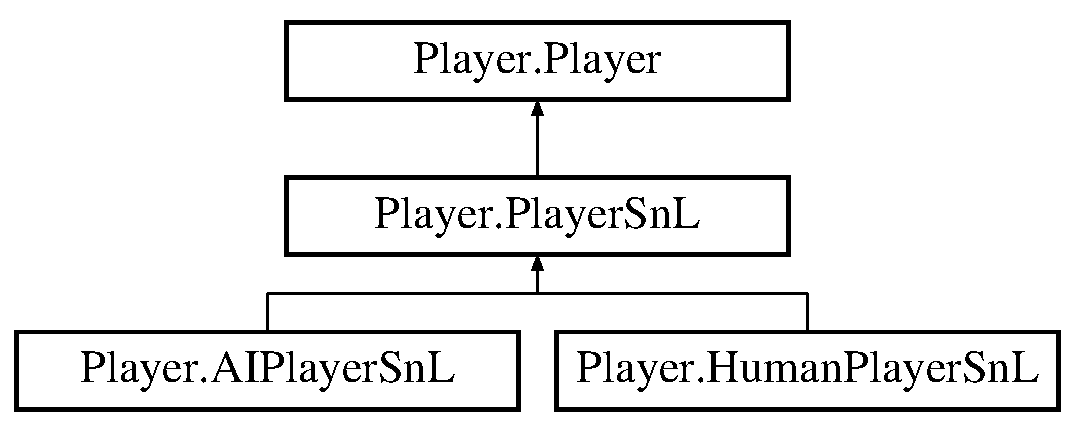
\includegraphics[height=3.000000cm]{class_player_1_1_player_sn_l}
\end{center}
\end{figure}
\subsection*{Public Member Functions}
\begin{DoxyCompactItemize}
\item 
int \hyperlink{class_player_1_1_player_sn_l_a36a358c20cb0f45cc87e7975befebbcc}{get\+Player\+Location} ()
\item 
Color \hyperlink{class_player_1_1_player_sn_l_a7d5b12033c99b19fda1be39e30470b2c}{get\+Player\+Color} ()
\item 
boolean \hyperlink{class_player_1_1_player_sn_l_a0b10f61660837878f6d3b9306b9cc8f3}{set\+Player\+Location} (\hyperlink{class_display_1_1_display_sn_l}{Display\+Sn\+L} display\+Sn\+L, \hyperlink{class_square_1_1_square}{Square} s, boolean \hyperlink{class_player_1_1_player_sn_l_a643b8e902d4c0701ead60eea0099107b}{is\+Movement\+Square})
\item 
void \hyperlink{class_player_1_1_player_sn_l_a31b9b469c7aabb27b5da8c38699587f3}{set\+Last\+Location} (int player\+Location)
\item 
int \hyperlink{class_player_1_1_player_sn_l_ac13c20e8675be07704620e1e54e714cc}{get\+Last\+Location} ()
\item 
Array\+List$<$ Integer $>$ \hyperlink{class_player_1_1_player_sn_l_a2f2c8d17959786a2c6ed0770fdf2d4df}{get\+All\+Locations} ()
\item 
boolean \hyperlink{class_player_1_1_player_sn_l_a643b8e902d4c0701ead60eea0099107b}{is\+Movement\+Square} (\hyperlink{class_square_1_1_square_sn_l}{Square\+Sn\+L} s)
\end{DoxyCompactItemize}
\subsection*{Public Attributes}
\begin{DoxyCompactItemize}
\item 
int \hyperlink{class_player_1_1_player_sn_l_a9ff667423ca24b7b21b9775117156d68}{m\+\_\+player\+Location} = 1
\item 
Color \hyperlink{class_player_1_1_player_sn_l_a9fb98bcd7461b8b5a3193ecc8d00fcaa}{m\+\_\+player\+Color}
\item 
boolean \hyperlink{class_player_1_1_player_sn_l_a41a8f9cd3f8340cccedd9393a8698477}{m\+\_\+is\+Movement\+On\+Square}
\item 
int \hyperlink{class_player_1_1_player_sn_l_a67ec420adf012813b5b6bf74237e0180}{m\+\_\+last\+Location}
\item 
Array\+List$<$ Integer $>$ \hyperlink{class_player_1_1_player_sn_l_a592990cc22e4082b31cae3e31124fcd6}{m\+\_\+all\+Locations} = new Array\+List$<$Integer$>$()
\end{DoxyCompactItemize}
\subsection*{Additional Inherited Members}


\subsection{Detailed Description}
Creates a player for Snakes and Ladders. 

\subsection{Member Function Documentation}
\hypertarget{class_player_1_1_player_sn_l_a2f2c8d17959786a2c6ed0770fdf2d4df}{}\index{Player\+::\+Player\+Sn\+L@{Player\+::\+Player\+Sn\+L}!get\+All\+Locations@{get\+All\+Locations}}
\index{get\+All\+Locations@{get\+All\+Locations}!Player\+::\+Player\+Sn\+L@{Player\+::\+Player\+Sn\+L}}
\subsubsection[{get\+All\+Locations()}]{\setlength{\rightskip}{0pt plus 5cm}Array\+List$<$Integer$>$ Player.\+Player\+Sn\+L.\+get\+All\+Locations (
\begin{DoxyParamCaption}
{}
\end{DoxyParamCaption}
)}\label{class_player_1_1_player_sn_l_a2f2c8d17959786a2c6ed0770fdf2d4df}
\hypertarget{class_player_1_1_player_sn_l_ac13c20e8675be07704620e1e54e714cc}{}\index{Player\+::\+Player\+Sn\+L@{Player\+::\+Player\+Sn\+L}!get\+Last\+Location@{get\+Last\+Location}}
\index{get\+Last\+Location@{get\+Last\+Location}!Player\+::\+Player\+Sn\+L@{Player\+::\+Player\+Sn\+L}}
\subsubsection[{get\+Last\+Location()}]{\setlength{\rightskip}{0pt plus 5cm}int Player.\+Player\+Sn\+L.\+get\+Last\+Location (
\begin{DoxyParamCaption}
{}
\end{DoxyParamCaption}
)}\label{class_player_1_1_player_sn_l_ac13c20e8675be07704620e1e54e714cc}
\hypertarget{class_player_1_1_player_sn_l_a7d5b12033c99b19fda1be39e30470b2c}{}\index{Player\+::\+Player\+Sn\+L@{Player\+::\+Player\+Sn\+L}!get\+Player\+Color@{get\+Player\+Color}}
\index{get\+Player\+Color@{get\+Player\+Color}!Player\+::\+Player\+Sn\+L@{Player\+::\+Player\+Sn\+L}}
\subsubsection[{get\+Player\+Color()}]{\setlength{\rightskip}{0pt plus 5cm}Color Player.\+Player\+Sn\+L.\+get\+Player\+Color (
\begin{DoxyParamCaption}
{}
\end{DoxyParamCaption}
)}\label{class_player_1_1_player_sn_l_a7d5b12033c99b19fda1be39e30470b2c}
get the piece color of player

\begin{DoxyReturn}{Returns}
piece color 
\end{DoxyReturn}
\hypertarget{class_player_1_1_player_sn_l_a36a358c20cb0f45cc87e7975befebbcc}{}\index{Player\+::\+Player\+Sn\+L@{Player\+::\+Player\+Sn\+L}!get\+Player\+Location@{get\+Player\+Location}}
\index{get\+Player\+Location@{get\+Player\+Location}!Player\+::\+Player\+Sn\+L@{Player\+::\+Player\+Sn\+L}}
\subsubsection[{get\+Player\+Location()}]{\setlength{\rightskip}{0pt plus 5cm}int Player.\+Player\+Sn\+L.\+get\+Player\+Location (
\begin{DoxyParamCaption}
{}
\end{DoxyParamCaption}
)}\label{class_player_1_1_player_sn_l_a36a358c20cb0f45cc87e7975befebbcc}
get the current piece location

\begin{DoxyReturn}{Returns}
current piece location 
\end{DoxyReturn}
\hypertarget{class_player_1_1_player_sn_l_a643b8e902d4c0701ead60eea0099107b}{}\index{Player\+::\+Player\+Sn\+L@{Player\+::\+Player\+Sn\+L}!is\+Movement\+Square@{is\+Movement\+Square}}
\index{is\+Movement\+Square@{is\+Movement\+Square}!Player\+::\+Player\+Sn\+L@{Player\+::\+Player\+Sn\+L}}
\subsubsection[{is\+Movement\+Square(\+Square\+Sn\+L s)}]{\setlength{\rightskip}{0pt plus 5cm}boolean Player.\+Player\+Sn\+L.\+is\+Movement\+Square (
\begin{DoxyParamCaption}
\item[{{\bf Square\+Sn\+L}}]{s}
\end{DoxyParamCaption}
)}\label{class_player_1_1_player_sn_l_a643b8e902d4c0701ead60eea0099107b}
check if the piece has moved to destination square


\begin{DoxyParams}{Parameters}
{\em s} & is destination square \\
\hline
\end{DoxyParams}
\begin{DoxyReturn}{Returns}
true if piece gets to destination square, or false if not 
\end{DoxyReturn}
\hypertarget{class_player_1_1_player_sn_l_a31b9b469c7aabb27b5da8c38699587f3}{}\index{Player\+::\+Player\+Sn\+L@{Player\+::\+Player\+Sn\+L}!set\+Last\+Location@{set\+Last\+Location}}
\index{set\+Last\+Location@{set\+Last\+Location}!Player\+::\+Player\+Sn\+L@{Player\+::\+Player\+Sn\+L}}
\subsubsection[{set\+Last\+Location(int player\+Location)}]{\setlength{\rightskip}{0pt plus 5cm}void Player.\+Player\+Sn\+L.\+set\+Last\+Location (
\begin{DoxyParamCaption}
\item[{int}]{player\+Location}
\end{DoxyParamCaption}
)}\label{class_player_1_1_player_sn_l_a31b9b469c7aabb27b5da8c38699587f3}
\hypertarget{class_player_1_1_player_sn_l_a0b10f61660837878f6d3b9306b9cc8f3}{}\index{Player\+::\+Player\+Sn\+L@{Player\+::\+Player\+Sn\+L}!set\+Player\+Location@{set\+Player\+Location}}
\index{set\+Player\+Location@{set\+Player\+Location}!Player\+::\+Player\+Sn\+L@{Player\+::\+Player\+Sn\+L}}
\subsubsection[{set\+Player\+Location(\+Display\+Sn\+L display\+Sn\+L, Square s, boolean is\+Movement\+Square)}]{\setlength{\rightskip}{0pt plus 5cm}boolean Player.\+Player\+Sn\+L.\+set\+Player\+Location (
\begin{DoxyParamCaption}
\item[{{\bf Display\+Sn\+L}}]{display\+Sn\+L, }
\item[{{\bf Square}}]{s, }
\item[{boolean}]{is\+Movement\+Square}
\end{DoxyParamCaption}
)}\label{class_player_1_1_player_sn_l_a0b10f61660837878f6d3b9306b9cc8f3}
if destination square is in the bound then move the piece to destination square


\begin{DoxyParams}{Parameters}
{\em display\+Sn\+L} & is current all game information \\
\hline
{\em s} & is destination square \\
\hline
{\em is\+Movement\+Square} & to check if the piece is on the destination square or not \\
\hline
\end{DoxyParams}
\begin{DoxyReturn}{Returns}
true if piece gets to destination square, or false if the destination is out of bound 
\end{DoxyReturn}


\subsection{Member Data Documentation}
\hypertarget{class_player_1_1_player_sn_l_a592990cc22e4082b31cae3e31124fcd6}{}\index{Player\+::\+Player\+Sn\+L@{Player\+::\+Player\+Sn\+L}!m\+\_\+all\+Locations@{m\+\_\+all\+Locations}}
\index{m\+\_\+all\+Locations@{m\+\_\+all\+Locations}!Player\+::\+Player\+Sn\+L@{Player\+::\+Player\+Sn\+L}}
\subsubsection[{m\+\_\+all\+Locations}]{\setlength{\rightskip}{0pt plus 5cm}Array\+List$<$Integer$>$ Player.\+Player\+Sn\+L.\+m\+\_\+all\+Locations = new Array\+List$<$Integer$>$()}\label{class_player_1_1_player_sn_l_a592990cc22e4082b31cae3e31124fcd6}
Array of positions \hypertarget{class_player_1_1_player_sn_l_a41a8f9cd3f8340cccedd9393a8698477}{}\index{Player\+::\+Player\+Sn\+L@{Player\+::\+Player\+Sn\+L}!m\+\_\+is\+Movement\+On\+Square@{m\+\_\+is\+Movement\+On\+Square}}
\index{m\+\_\+is\+Movement\+On\+Square@{m\+\_\+is\+Movement\+On\+Square}!Player\+::\+Player\+Sn\+L@{Player\+::\+Player\+Sn\+L}}
\subsubsection[{m\+\_\+is\+Movement\+On\+Square}]{\setlength{\rightskip}{0pt plus 5cm}boolean Player.\+Player\+Sn\+L.\+m\+\_\+is\+Movement\+On\+Square}\label{class_player_1_1_player_sn_l_a41a8f9cd3f8340cccedd9393a8698477}
To check if piece is on the destination square or not \hypertarget{class_player_1_1_player_sn_l_a67ec420adf012813b5b6bf74237e0180}{}\index{Player\+::\+Player\+Sn\+L@{Player\+::\+Player\+Sn\+L}!m\+\_\+last\+Location@{m\+\_\+last\+Location}}
\index{m\+\_\+last\+Location@{m\+\_\+last\+Location}!Player\+::\+Player\+Sn\+L@{Player\+::\+Player\+Sn\+L}}
\subsubsection[{m\+\_\+last\+Location}]{\setlength{\rightskip}{0pt plus 5cm}int Player.\+Player\+Sn\+L.\+m\+\_\+last\+Location}\label{class_player_1_1_player_sn_l_a67ec420adf012813b5b6bf74237e0180}
Last location of player \hypertarget{class_player_1_1_player_sn_l_a9fb98bcd7461b8b5a3193ecc8d00fcaa}{}\index{Player\+::\+Player\+Sn\+L@{Player\+::\+Player\+Sn\+L}!m\+\_\+player\+Color@{m\+\_\+player\+Color}}
\index{m\+\_\+player\+Color@{m\+\_\+player\+Color}!Player\+::\+Player\+Sn\+L@{Player\+::\+Player\+Sn\+L}}
\subsubsection[{m\+\_\+player\+Color}]{\setlength{\rightskip}{0pt plus 5cm}Color Player.\+Player\+Sn\+L.\+m\+\_\+player\+Color}\label{class_player_1_1_player_sn_l_a9fb98bcd7461b8b5a3193ecc8d00fcaa}
The piece color of the player \hypertarget{class_player_1_1_player_sn_l_a9ff667423ca24b7b21b9775117156d68}{}\index{Player\+::\+Player\+Sn\+L@{Player\+::\+Player\+Sn\+L}!m\+\_\+player\+Location@{m\+\_\+player\+Location}}
\index{m\+\_\+player\+Location@{m\+\_\+player\+Location}!Player\+::\+Player\+Sn\+L@{Player\+::\+Player\+Sn\+L}}
\subsubsection[{m\+\_\+player\+Location}]{\setlength{\rightskip}{0pt plus 5cm}int Player.\+Player\+Sn\+L.\+m\+\_\+player\+Location = 1}\label{class_player_1_1_player_sn_l_a9ff667423ca24b7b21b9775117156d68}
The piece initial location of the player 

The documentation for this class was generated from the following file\+:\begin{DoxyCompactItemize}
\item 
src/\+Player/\hyperlink{_player_sn_l_8java}{Player\+Sn\+L.\+java}\end{DoxyCompactItemize}

\hypertarget{class_player_1_1_player_t_t_t}{}\section{Player.\+Player\+T\+T\+T Class Reference}
\label{class_player_1_1_player_t_t_t}\index{Player.\+Player\+T\+T\+T@{Player.\+Player\+T\+T\+T}}


Creates a player for Tic\+Tac\+Toe.  


Inheritance diagram for Player.\+Player\+T\+T\+T\+:\begin{figure}[H]
\begin{center}
\leavevmode
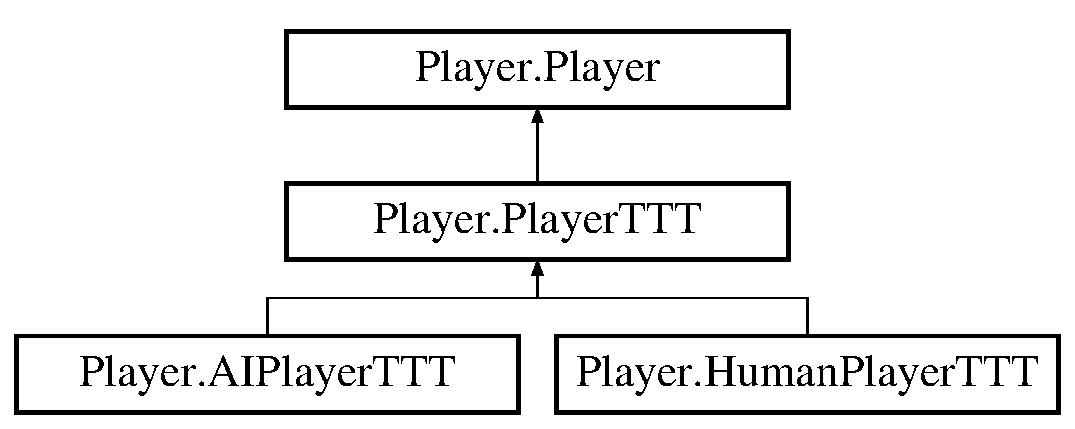
\includegraphics[height=3.000000cm]{class_player_1_1_player_t_t_t}
\end{center}
\end{figure}
\subsection*{Public Member Functions}
\begin{DoxyCompactItemize}
\item 
char \hyperlink{class_player_1_1_player_t_t_t_ab8b6942da0005040404d3ac02c71e463}{get\+Player\+Piece\+Type} ()
\item 
void \hyperlink{class_player_1_1_player_t_t_t_ae624b6b5a46f011a667e0562ad150091}{set\+Player\+Piece\+Type} (char player\+Type)
\item 
Array\+List$<$ Integer $>$ \hyperlink{class_player_1_1_player_t_t_t_a491c3a16684131362d6808e4827d566e}{get\+Piece\+Locations} ()
\item 
int \hyperlink{class_player_1_1_player_t_t_t_aee939d68fa0f319d0e6101a9373e7c7e}{get\+Piece\+Location} ()
\item 
boolean \hyperlink{class_player_1_1_player_t_t_t_ace718e5b67209360615144048fd1814a}{is\+X} ()
\item 
boolean \hyperlink{class_player_1_1_player_t_t_t_ac3f8f41bc0b24865c80283d5a84be6d4}{is\+O} ()
\item 
void \hyperlink{class_player_1_1_player_t_t_t_ab3d884c71bcd92b42bea5a413caa95e8}{add\+Piece} (\hyperlink{class_square_1_1_square}{Square} s)
\end{DoxyCompactItemize}
\subsection*{Static Public Member Functions}
\begin{DoxyCompactItemize}
\item 
static void \hyperlink{class_player_1_1_player_t_t_t_a408aa90bd0399d51f36e9fd621ab4374}{main} (String\mbox{[}$\,$\mbox{]} args)
\end{DoxyCompactItemize}
\subsection*{Private Attributes}
\begin{DoxyCompactItemize}
\item 
char \hyperlink{class_player_1_1_player_t_t_t_a2fa13b6b056d666ea9943ca84862ec69}{m\+\_\+piece\+Type}
\item 
Array\+List$<$ Integer $>$ \hyperlink{class_player_1_1_player_t_t_t_a5416049a939a127279680881a54a21d2}{m\+\_\+piece\+Locations} =new Array\+List$<$Integer$>$()
\end{DoxyCompactItemize}


\subsection{Detailed Description}
Creates a player for Tic\+Tac\+Toe. 

\subsection{Member Function Documentation}
\hypertarget{class_player_1_1_player_t_t_t_ab3d884c71bcd92b42bea5a413caa95e8}{}\index{Player\+::\+Player\+T\+T\+T@{Player\+::\+Player\+T\+T\+T}!add\+Piece@{add\+Piece}}
\index{add\+Piece@{add\+Piece}!Player\+::\+Player\+T\+T\+T@{Player\+::\+Player\+T\+T\+T}}
\subsubsection[{add\+Piece(\+Square s)}]{\setlength{\rightskip}{0pt plus 5cm}void Player.\+Player\+T\+T\+T.\+add\+Piece (
\begin{DoxyParamCaption}
\item[{{\bf Square}}]{s}
\end{DoxyParamCaption}
)}\label{class_player_1_1_player_t_t_t_ab3d884c71bcd92b42bea5a413caa95e8}
Add Piece to Piece array 
\begin{DoxyParams}{Parameters}
{\em s} & the square location you put the piece on \\
\hline
\end{DoxyParams}
\hypertarget{class_player_1_1_player_t_t_t_aee939d68fa0f319d0e6101a9373e7c7e}{}\index{Player\+::\+Player\+T\+T\+T@{Player\+::\+Player\+T\+T\+T}!get\+Piece\+Location@{get\+Piece\+Location}}
\index{get\+Piece\+Location@{get\+Piece\+Location}!Player\+::\+Player\+T\+T\+T@{Player\+::\+Player\+T\+T\+T}}
\subsubsection[{get\+Piece\+Location()}]{\setlength{\rightskip}{0pt plus 5cm}int Player.\+Player\+T\+T\+T.\+get\+Piece\+Location (
\begin{DoxyParamCaption}
{}
\end{DoxyParamCaption}
)}\label{class_player_1_1_player_t_t_t_aee939d68fa0f319d0e6101a9373e7c7e}
get the every piece location integer from 0 to size-\/1 \begin{DoxyReturn}{Returns}
most recently placed piece 
\end{DoxyReturn}
\hypertarget{class_player_1_1_player_t_t_t_a491c3a16684131362d6808e4827d566e}{}\index{Player\+::\+Player\+T\+T\+T@{Player\+::\+Player\+T\+T\+T}!get\+Piece\+Locations@{get\+Piece\+Locations}}
\index{get\+Piece\+Locations@{get\+Piece\+Locations}!Player\+::\+Player\+T\+T\+T@{Player\+::\+Player\+T\+T\+T}}
\subsubsection[{get\+Piece\+Locations()}]{\setlength{\rightskip}{0pt plus 5cm}Array\+List$<$Integer$>$ Player.\+Player\+T\+T\+T.\+get\+Piece\+Locations (
\begin{DoxyParamCaption}
{}
\end{DoxyParamCaption}
)}\label{class_player_1_1_player_t_t_t_a491c3a16684131362d6808e4827d566e}
\begin{DoxyReturn}{Returns}
full set of piece locations 
\end{DoxyReturn}
\hypertarget{class_player_1_1_player_t_t_t_ab8b6942da0005040404d3ac02c71e463}{}\index{Player\+::\+Player\+T\+T\+T@{Player\+::\+Player\+T\+T\+T}!get\+Player\+Piece\+Type@{get\+Player\+Piece\+Type}}
\index{get\+Player\+Piece\+Type@{get\+Player\+Piece\+Type}!Player\+::\+Player\+T\+T\+T@{Player\+::\+Player\+T\+T\+T}}
\subsubsection[{get\+Player\+Piece\+Type()}]{\setlength{\rightskip}{0pt plus 5cm}char Player.\+Player\+T\+T\+T.\+get\+Player\+Piece\+Type (
\begin{DoxyParamCaption}
{}
\end{DoxyParamCaption}
)}\label{class_player_1_1_player_t_t_t_ab8b6942da0005040404d3ac02c71e463}
Gets the player piece type \begin{DoxyReturn}{Returns}
the player piece type is X or O 
\end{DoxyReturn}
\hypertarget{class_player_1_1_player_t_t_t_ac3f8f41bc0b24865c80283d5a84be6d4}{}\index{Player\+::\+Player\+T\+T\+T@{Player\+::\+Player\+T\+T\+T}!is\+O@{is\+O}}
\index{is\+O@{is\+O}!Player\+::\+Player\+T\+T\+T@{Player\+::\+Player\+T\+T\+T}}
\subsubsection[{is\+O()}]{\setlength{\rightskip}{0pt plus 5cm}boolean Player.\+Player\+T\+T\+T.\+is\+O (
\begin{DoxyParamCaption}
{}
\end{DoxyParamCaption}
)}\label{class_player_1_1_player_t_t_t_ac3f8f41bc0b24865c80283d5a84be6d4}
Check if the player piece is O or not \begin{DoxyReturn}{Returns}
the true if player\+Piece\+Type is O 
\end{DoxyReturn}
\hypertarget{class_player_1_1_player_t_t_t_ace718e5b67209360615144048fd1814a}{}\index{Player\+::\+Player\+T\+T\+T@{Player\+::\+Player\+T\+T\+T}!is\+X@{is\+X}}
\index{is\+X@{is\+X}!Player\+::\+Player\+T\+T\+T@{Player\+::\+Player\+T\+T\+T}}
\subsubsection[{is\+X()}]{\setlength{\rightskip}{0pt plus 5cm}boolean Player.\+Player\+T\+T\+T.\+is\+X (
\begin{DoxyParamCaption}
{}
\end{DoxyParamCaption}
)}\label{class_player_1_1_player_t_t_t_ace718e5b67209360615144048fd1814a}
Check if the player piece is X or not \begin{DoxyReturn}{Returns}
the true if player\+Piece\+Type is X 
\end{DoxyReturn}
\hypertarget{class_player_1_1_player_t_t_t_a408aa90bd0399d51f36e9fd621ab4374}{}\index{Player\+::\+Player\+T\+T\+T@{Player\+::\+Player\+T\+T\+T}!main@{main}}
\index{main@{main}!Player\+::\+Player\+T\+T\+T@{Player\+::\+Player\+T\+T\+T}}
\subsubsection[{main(\+String[] args)}]{\setlength{\rightskip}{0pt plus 5cm}static void Player.\+Player\+T\+T\+T.\+main (
\begin{DoxyParamCaption}
\item[{String   \mbox{[}$\,$\mbox{]}}]{args}
\end{DoxyParamCaption}
)\hspace{0.3cm}{\ttfamily [static]}}\label{class_player_1_1_player_t_t_t_a408aa90bd0399d51f36e9fd621ab4374}
main method created for unit testing 
\begin{DoxyParams}{Parameters}
{\em args} & \\
\hline
\end{DoxyParams}
\hypertarget{class_player_1_1_player_t_t_t_ae624b6b5a46f011a667e0562ad150091}{}\index{Player\+::\+Player\+T\+T\+T@{Player\+::\+Player\+T\+T\+T}!set\+Player\+Piece\+Type@{set\+Player\+Piece\+Type}}
\index{set\+Player\+Piece\+Type@{set\+Player\+Piece\+Type}!Player\+::\+Player\+T\+T\+T@{Player\+::\+Player\+T\+T\+T}}
\subsubsection[{set\+Player\+Piece\+Type(char player\+Type)}]{\setlength{\rightskip}{0pt plus 5cm}void Player.\+Player\+T\+T\+T.\+set\+Player\+Piece\+Type (
\begin{DoxyParamCaption}
\item[{char}]{player\+Type}
\end{DoxyParamCaption}
)}\label{class_player_1_1_player_t_t_t_ae624b6b5a46f011a667e0562ad150091}
Sets the player piece type \begin{DoxyReturn}{Returns}
the player piece type 
\end{DoxyReturn}


\subsection{Member Data Documentation}
\hypertarget{class_player_1_1_player_t_t_t_a5416049a939a127279680881a54a21d2}{}\index{Player\+::\+Player\+T\+T\+T@{Player\+::\+Player\+T\+T\+T}!m\+\_\+piece\+Locations@{m\+\_\+piece\+Locations}}
\index{m\+\_\+piece\+Locations@{m\+\_\+piece\+Locations}!Player\+::\+Player\+T\+T\+T@{Player\+::\+Player\+T\+T\+T}}
\subsubsection[{m\+\_\+piece\+Locations}]{\setlength{\rightskip}{0pt plus 5cm}Array\+List$<$Integer$>$ Player.\+Player\+T\+T\+T.\+m\+\_\+piece\+Locations =new Array\+List$<$Integer$>$()\hspace{0.3cm}{\ttfamily [private]}}\label{class_player_1_1_player_t_t_t_a5416049a939a127279680881a54a21d2}
The piece location array of the player \hypertarget{class_player_1_1_player_t_t_t_a2fa13b6b056d666ea9943ca84862ec69}{}\index{Player\+::\+Player\+T\+T\+T@{Player\+::\+Player\+T\+T\+T}!m\+\_\+piece\+Type@{m\+\_\+piece\+Type}}
\index{m\+\_\+piece\+Type@{m\+\_\+piece\+Type}!Player\+::\+Player\+T\+T\+T@{Player\+::\+Player\+T\+T\+T}}
\subsubsection[{m\+\_\+piece\+Type}]{\setlength{\rightskip}{0pt plus 5cm}char Player.\+Player\+T\+T\+T.\+m\+\_\+piece\+Type\hspace{0.3cm}{\ttfamily [private]}}\label{class_player_1_1_player_t_t_t_a2fa13b6b056d666ea9943ca84862ec69}
The piece type of the player 

The documentation for this class was generated from the following file\+:\begin{DoxyCompactItemize}
\item 
src/\+Player/\hyperlink{_player_t_t_t_8java}{Player\+T\+T\+T.\+java}\end{DoxyCompactItemize}

\hypertarget{class_square_1_1_square}{}\section{Square.\+Square Class Reference}
\label{class_square_1_1_square}\index{Square.\+Square@{Square.\+Square}}
Inheritance diagram for Square.\+Square\+:\begin{figure}[H]
\begin{center}
\leavevmode
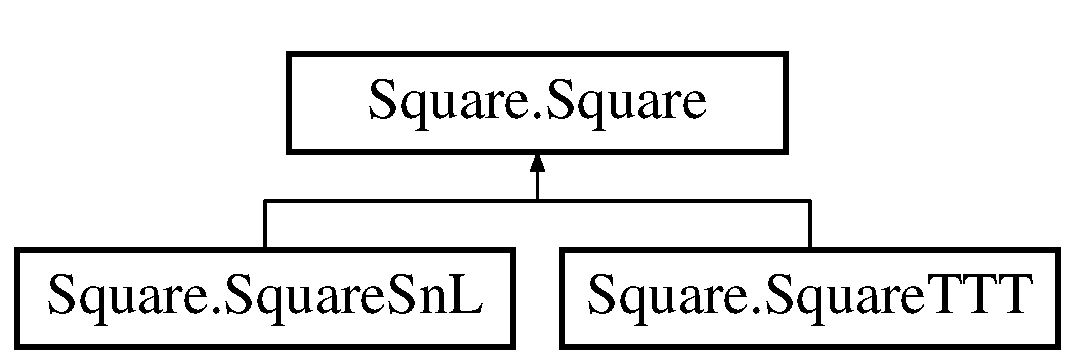
\includegraphics[height=2.000000cm]{class_square_1_1_square}
\end{center}
\end{figure}
\subsection*{Public Member Functions}
\begin{DoxyCompactItemize}
\item 
void \hyperlink{class_square_1_1_square_a660b369288339117bda29e9a47dae8f6}{set\+Value} (char x)
\item 
char \hyperlink{class_square_1_1_square_a0afb61e6814c61ae2036b15a1a958e6f}{get\+Value} ()
\item 
int \hyperlink{class_square_1_1_square_a270f9a35b0432406d2464201ece4c6b0}{get\+Position} ()
\item 
String \hyperlink{class_square_1_1_square_ab94a6f61d25fde4e49055fcb09d6f33a}{to\+String} ()
\end{DoxyCompactItemize}
\subsection*{Protected Attributes}
\begin{DoxyCompactItemize}
\item 
int \hyperlink{class_square_1_1_square_a459ef3208bfff1bc1a693a335c2cd5e5}{m\+\_\+position}
\item 
char \hyperlink{class_square_1_1_square_a9e0779af7f8cbe54b28f95bb4a5d165a}{m\+\_\+x}
\end{DoxyCompactItemize}


\subsection{Member Function Documentation}
\hypertarget{class_square_1_1_square_a270f9a35b0432406d2464201ece4c6b0}{}\index{Square\+::\+Square@{Square\+::\+Square}!get\+Position@{get\+Position}}
\index{get\+Position@{get\+Position}!Square\+::\+Square@{Square\+::\+Square}}
\subsubsection[{get\+Position()}]{\setlength{\rightskip}{0pt plus 5cm}int Square.\+Square.\+get\+Position (
\begin{DoxyParamCaption}
{}
\end{DoxyParamCaption}
)}\label{class_square_1_1_square_a270f9a35b0432406d2464201ece4c6b0}
Gets the position of the squares \begin{DoxyReturn}{Returns}
position 
\end{DoxyReturn}
\hypertarget{class_square_1_1_square_a0afb61e6814c61ae2036b15a1a958e6f}{}\index{Square\+::\+Square@{Square\+::\+Square}!get\+Value@{get\+Value}}
\index{get\+Value@{get\+Value}!Square\+::\+Square@{Square\+::\+Square}}
\subsubsection[{get\+Value()}]{\setlength{\rightskip}{0pt plus 5cm}char Square.\+Square.\+get\+Value (
\begin{DoxyParamCaption}
{}
\end{DoxyParamCaption}
)}\label{class_square_1_1_square_a0afb61e6814c61ae2036b15a1a958e6f}
Gets value for x \begin{DoxyReturn}{Returns}
x 
\end{DoxyReturn}
\hypertarget{class_square_1_1_square_a660b369288339117bda29e9a47dae8f6}{}\index{Square\+::\+Square@{Square\+::\+Square}!set\+Value@{set\+Value}}
\index{set\+Value@{set\+Value}!Square\+::\+Square@{Square\+::\+Square}}
\subsubsection[{set\+Value(char x)}]{\setlength{\rightskip}{0pt plus 5cm}void Square.\+Square.\+set\+Value (
\begin{DoxyParamCaption}
\item[{char}]{x}
\end{DoxyParamCaption}
)}\label{class_square_1_1_square_a660b369288339117bda29e9a47dae8f6}
Sets the values for x 
\begin{DoxyParams}{Parameters}
{\em x} & \\
\hline
\end{DoxyParams}
\hypertarget{class_square_1_1_square_ab94a6f61d25fde4e49055fcb09d6f33a}{}\index{Square\+::\+Square@{Square\+::\+Square}!to\+String@{to\+String}}
\index{to\+String@{to\+String}!Square\+::\+Square@{Square\+::\+Square}}
\subsubsection[{to\+String()}]{\setlength{\rightskip}{0pt plus 5cm}String Square.\+Square.\+to\+String (
\begin{DoxyParamCaption}
{}
\end{DoxyParamCaption}
)}\label{class_square_1_1_square_ab94a6f61d25fde4e49055fcb09d6f33a}
Gets the position of the square and converts it to a string

\begin{DoxyReturn}{Returns}
the position of s as a string 
\end{DoxyReturn}


\subsection{Member Data Documentation}
\hypertarget{class_square_1_1_square_a459ef3208bfff1bc1a693a335c2cd5e5}{}\index{Square\+::\+Square@{Square\+::\+Square}!m\+\_\+position@{m\+\_\+position}}
\index{m\+\_\+position@{m\+\_\+position}!Square\+::\+Square@{Square\+::\+Square}}
\subsubsection[{m\+\_\+position}]{\setlength{\rightskip}{0pt plus 5cm}int Square.\+Square.\+m\+\_\+position\hspace{0.3cm}{\ttfamily [protected]}}\label{class_square_1_1_square_a459ef3208bfff1bc1a693a335c2cd5e5}
Stores the position of the square on the board \hypertarget{class_square_1_1_square_a9e0779af7f8cbe54b28f95bb4a5d165a}{}\index{Square\+::\+Square@{Square\+::\+Square}!m\+\_\+x@{m\+\_\+x}}
\index{m\+\_\+x@{m\+\_\+x}!Square\+::\+Square@{Square\+::\+Square}}
\subsubsection[{m\+\_\+x}]{\setlength{\rightskip}{0pt plus 5cm}char Square.\+Square.\+m\+\_\+x\hspace{0.3cm}{\ttfamily [protected]}}\label{class_square_1_1_square_a9e0779af7f8cbe54b28f95bb4a5d165a}
Stores what the square is filled with. possible values\+: \char`\"{} \char`\"{}, \char`\"{}\+O\char`\"{} or \char`\"{}\+X\char`\"{} 

The documentation for this class was generated from the following file\+:\begin{DoxyCompactItemize}
\item 
src/\+Square/\hyperlink{_square_8java}{Square.\+java}\end{DoxyCompactItemize}

\hypertarget{class_square_1_1_square_sn_l}{}\section{Square.\+Square\+Sn\+L Class Reference}
\label{class_square_1_1_square_sn_l}\index{Square.\+Square\+Sn\+L@{Square.\+Square\+Sn\+L}}


This class stores the information on each square for Sn\+L.  


Inheritance diagram for Square.\+Square\+Sn\+L\+:\begin{figure}[H]
\begin{center}
\leavevmode
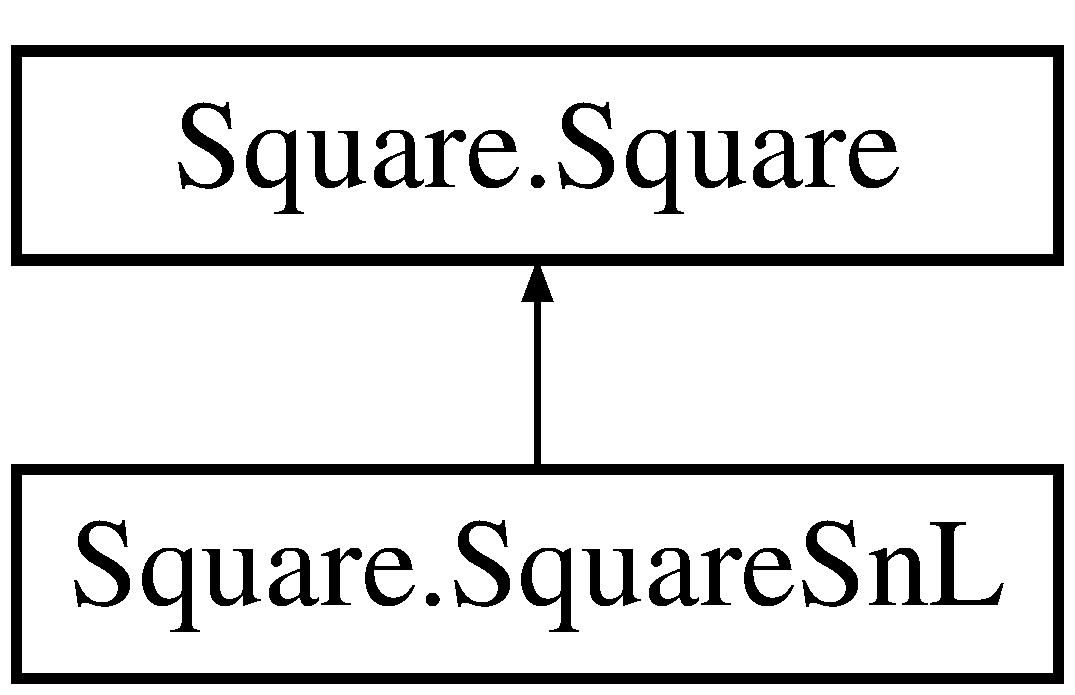
\includegraphics[height=2.000000cm]{class_square_1_1_square_sn_l}
\end{center}
\end{figure}
\subsection*{Public Member Functions}
\begin{DoxyCompactItemize}
\item 
\hyperlink{class_square_1_1_square_sn_l_ac89482de8a579e2b2249f9d8bf652351}{Square\+Sn\+L} (int position, int destination)
\item 
int \hyperlink{class_square_1_1_square_sn_l_acb377b2ceb8dd5b8d65bba391f4c256d}{get\+Destination} ()
\item 
boolean \hyperlink{class_square_1_1_square_sn_l_ad948a877cff45a872082f23d72924770}{is\+Movement\+Square} ()
\item 
boolean \hyperlink{class_square_1_1_square_sn_l_a7f23505690a2a6ccfe9126448f66ddeb}{exists\+Player} ()
\end{DoxyCompactItemize}
\subsection*{Static Public Member Functions}
\begin{DoxyCompactItemize}
\item 
static void \hyperlink{class_square_1_1_square_sn_l_ac30c492a8a5c6f0f9bf43faa069dfa5c}{main} (String\mbox{[}$\,$\mbox{]} args)
\end{DoxyCompactItemize}
\subsection*{Private Attributes}
\begin{DoxyCompactItemize}
\item 
int \hyperlink{class_square_1_1_square_sn_l_a1906be8d7e5ea28a4b5b1585d820186f}{m\+\_\+destination}
\end{DoxyCompactItemize}
\subsection*{Additional Inherited Members}


\subsection{Detailed Description}
This class stores the information on each square for Sn\+L. 

\subsection{Constructor \& Destructor Documentation}
\hypertarget{class_square_1_1_square_sn_l_ac89482de8a579e2b2249f9d8bf652351}{}\index{Square\+::\+Square\+Sn\+L@{Square\+::\+Square\+Sn\+L}!Square\+Sn\+L@{Square\+Sn\+L}}
\index{Square\+Sn\+L@{Square\+Sn\+L}!Square\+::\+Square\+Sn\+L@{Square\+::\+Square\+Sn\+L}}
\subsubsection[{Square\+Sn\+L(int position, int destination)}]{\setlength{\rightskip}{0pt plus 5cm}Square.\+Square\+Sn\+L.\+Square\+Sn\+L (
\begin{DoxyParamCaption}
\item[{int}]{position, }
\item[{int}]{destination}
\end{DoxyParamCaption}
)}\label{class_square_1_1_square_sn_l_ac89482de8a579e2b2249f9d8bf652351}
Sets up the square with the position and destination 
\begin{DoxyParams}{Parameters}
{\em position} & \\
\hline
{\em destination} & \\
\hline
\end{DoxyParams}


\subsection{Member Function Documentation}
\hypertarget{class_square_1_1_square_sn_l_a7f23505690a2a6ccfe9126448f66ddeb}{}\index{Square\+::\+Square\+Sn\+L@{Square\+::\+Square\+Sn\+L}!exists\+Player@{exists\+Player}}
\index{exists\+Player@{exists\+Player}!Square\+::\+Square\+Sn\+L@{Square\+::\+Square\+Sn\+L}}
\subsubsection[{exists\+Player()}]{\setlength{\rightskip}{0pt plus 5cm}boolean Square.\+Square\+Sn\+L.\+exists\+Player (
\begin{DoxyParamCaption}
{}
\end{DoxyParamCaption}
)}\label{class_square_1_1_square_sn_l_a7f23505690a2a6ccfe9126448f66ddeb}
returns whether a player is in the square \begin{DoxyReturn}{Returns}
true if there is a player in the square, false if not 
\end{DoxyReturn}
\hypertarget{class_square_1_1_square_sn_l_acb377b2ceb8dd5b8d65bba391f4c256d}{}\index{Square\+::\+Square\+Sn\+L@{Square\+::\+Square\+Sn\+L}!get\+Destination@{get\+Destination}}
\index{get\+Destination@{get\+Destination}!Square\+::\+Square\+Sn\+L@{Square\+::\+Square\+Sn\+L}}
\subsubsection[{get\+Destination()}]{\setlength{\rightskip}{0pt plus 5cm}int Square.\+Square\+Sn\+L.\+get\+Destination (
\begin{DoxyParamCaption}
{}
\end{DoxyParamCaption}
)}\label{class_square_1_1_square_sn_l_acb377b2ceb8dd5b8d65bba391f4c256d}
returns the destination of this square, possible that destination == position \begin{DoxyReturn}{Returns}
destination 
\end{DoxyReturn}
\hypertarget{class_square_1_1_square_sn_l_ad948a877cff45a872082f23d72924770}{}\index{Square\+::\+Square\+Sn\+L@{Square\+::\+Square\+Sn\+L}!is\+Movement\+Square@{is\+Movement\+Square}}
\index{is\+Movement\+Square@{is\+Movement\+Square}!Square\+::\+Square\+Sn\+L@{Square\+::\+Square\+Sn\+L}}
\subsubsection[{is\+Movement\+Square()}]{\setlength{\rightskip}{0pt plus 5cm}boolean Square.\+Square\+Sn\+L.\+is\+Movement\+Square (
\begin{DoxyParamCaption}
{}
\end{DoxyParamCaption}
)}\label{class_square_1_1_square_sn_l_ad948a877cff45a872082f23d72924770}
Returns whether this square is a movement square \begin{DoxyReturn}{Returns}
true if this square is a movement square, false if it is not 
\end{DoxyReturn}
\hypertarget{class_square_1_1_square_sn_l_ac30c492a8a5c6f0f9bf43faa069dfa5c}{}\index{Square\+::\+Square\+Sn\+L@{Square\+::\+Square\+Sn\+L}!main@{main}}
\index{main@{main}!Square\+::\+Square\+Sn\+L@{Square\+::\+Square\+Sn\+L}}
\subsubsection[{main(\+String[] args)}]{\setlength{\rightskip}{0pt plus 5cm}static void Square.\+Square\+Sn\+L.\+main (
\begin{DoxyParamCaption}
\item[{String\mbox{[}$\,$\mbox{]}}]{args}
\end{DoxyParamCaption}
)\hspace{0.3cm}{\ttfamily [static]}}\label{class_square_1_1_square_sn_l_ac30c492a8a5c6f0f9bf43faa069dfa5c}


\subsection{Member Data Documentation}
\hypertarget{class_square_1_1_square_sn_l_a1906be8d7e5ea28a4b5b1585d820186f}{}\index{Square\+::\+Square\+Sn\+L@{Square\+::\+Square\+Sn\+L}!m\+\_\+destination@{m\+\_\+destination}}
\index{m\+\_\+destination@{m\+\_\+destination}!Square\+::\+Square\+Sn\+L@{Square\+::\+Square\+Sn\+L}}
\subsubsection[{m\+\_\+destination}]{\setlength{\rightskip}{0pt plus 5cm}int Square.\+Square\+Sn\+L.\+m\+\_\+destination\hspace{0.3cm}{\ttfamily [private]}}\label{class_square_1_1_square_sn_l_a1906be8d7e5ea28a4b5b1585d820186f}
Stores the destination of this square if it is a movement square 

The documentation for this class was generated from the following file\+:\begin{DoxyCompactItemize}
\item 
src/\+Square/\hyperlink{_square_sn_l_8java}{Square\+Sn\+L.\+java}\end{DoxyCompactItemize}

\hypertarget{class_square_1_1_square_t_t_t}{}\section{Square.\+Square\+T\+T\+T Class Reference}
\label{class_square_1_1_square_t_t_t}\index{Square.\+Square\+T\+T\+T@{Square.\+Square\+T\+T\+T}}


This class stores the information on each square for T\+T\+T.  


Inheritance diagram for Square.\+Square\+T\+T\+T\+:\begin{figure}[H]
\begin{center}
\leavevmode
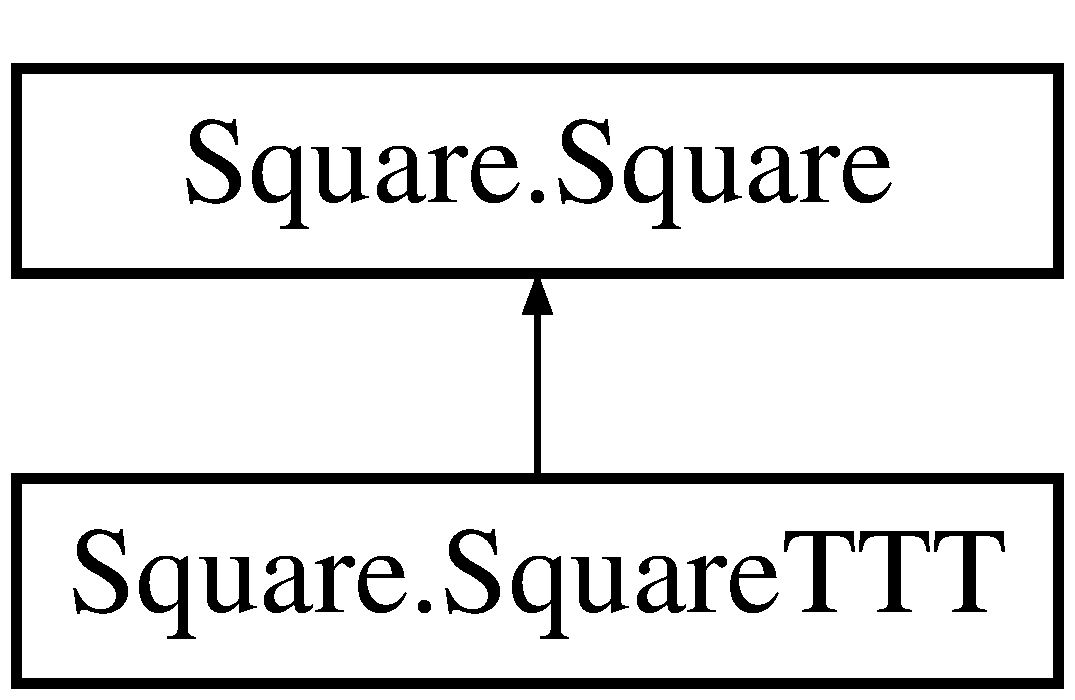
\includegraphics[height=2.000000cm]{class_square_1_1_square_t_t_t}
\end{center}
\end{figure}
\subsection*{Public Member Functions}
\begin{DoxyCompactItemize}
\item 
\hyperlink{class_square_1_1_square_t_t_t_a61856539b9717c3b5a3c6f46da3bb1a2}{Square\+T\+T\+T} (int i)
\item 
\hyperlink{class_square_1_1_square_t_t_t_aa369a31f4b3520bbbb7db02d31a11139}{Square\+T\+T\+T} (int i, char value, \hyperlink{class_display_1_1_display_t_t_t}{Display\+T\+T\+T} display)
\end{DoxyCompactItemize}
\subsection*{Static Public Member Functions}
\begin{DoxyCompactItemize}
\item 
static void \hyperlink{class_square_1_1_square_t_t_t_ad094b8dd8700576e4323fd69773dd6e9}{main} (String\mbox{[}$\,$\mbox{]} args)
\end{DoxyCompactItemize}
\subsection*{Additional Inherited Members}


\subsection{Detailed Description}
This class stores the information on each square for T\+T\+T. 

\subsection{Constructor \& Destructor Documentation}
\hypertarget{class_square_1_1_square_t_t_t_a61856539b9717c3b5a3c6f46da3bb1a2}{}\index{Square\+::\+Square\+T\+T\+T@{Square\+::\+Square\+T\+T\+T}!Square\+T\+T\+T@{Square\+T\+T\+T}}
\index{Square\+T\+T\+T@{Square\+T\+T\+T}!Square\+::\+Square\+T\+T\+T@{Square\+::\+Square\+T\+T\+T}}
\subsubsection[{Square\+T\+T\+T(int i)}]{\setlength{\rightskip}{0pt plus 5cm}Square.\+Square\+T\+T\+T.\+Square\+T\+T\+T (
\begin{DoxyParamCaption}
\item[{int}]{i}
\end{DoxyParamCaption}
)}\label{class_square_1_1_square_t_t_t_a61856539b9717c3b5a3c6f46da3bb1a2}
Constructor for setting up the squares in T\+T\+T 
\begin{DoxyParams}{Parameters}
{\em i} & \\
\hline
\end{DoxyParams}
\hypertarget{class_square_1_1_square_t_t_t_aa369a31f4b3520bbbb7db02d31a11139}{}\index{Square\+::\+Square\+T\+T\+T@{Square\+::\+Square\+T\+T\+T}!Square\+T\+T\+T@{Square\+T\+T\+T}}
\index{Square\+T\+T\+T@{Square\+T\+T\+T}!Square\+::\+Square\+T\+T\+T@{Square\+::\+Square\+T\+T\+T}}
\subsubsection[{Square\+T\+T\+T(int i, char value, Display\+T\+T\+T display)}]{\setlength{\rightskip}{0pt plus 5cm}Square.\+Square\+T\+T\+T.\+Square\+T\+T\+T (
\begin{DoxyParamCaption}
\item[{int}]{i, }
\item[{char}]{value, }
\item[{{\bf Display\+T\+T\+T}}]{display}
\end{DoxyParamCaption}
)}\label{class_square_1_1_square_t_t_t_aa369a31f4b3520bbbb7db02d31a11139}


\subsection{Member Function Documentation}
\hypertarget{class_square_1_1_square_t_t_t_ad094b8dd8700576e4323fd69773dd6e9}{}\index{Square\+::\+Square\+T\+T\+T@{Square\+::\+Square\+T\+T\+T}!main@{main}}
\index{main@{main}!Square\+::\+Square\+T\+T\+T@{Square\+::\+Square\+T\+T\+T}}
\subsubsection[{main(\+String[] args)}]{\setlength{\rightskip}{0pt plus 5cm}static void Square.\+Square\+T\+T\+T.\+main (
\begin{DoxyParamCaption}
\item[{String\mbox{[}$\,$\mbox{]}}]{args}
\end{DoxyParamCaption}
)\hspace{0.3cm}{\ttfamily [static]}}\label{class_square_1_1_square_t_t_t_ad094b8dd8700576e4323fd69773dd6e9}


The documentation for this class was generated from the following file\+:\begin{DoxyCompactItemize}
\item 
src/\+Square/\hyperlink{_square_t_t_t_8java}{Square\+T\+T\+T.\+java}\end{DoxyCompactItemize}

\chapter{File Documentation}
\hypertarget{_board_8java}{}\section{src/\+Board/\+Board.java File Reference}
\label{_board_8java}\index{src/\+Board/\+Board.\+java@{src/\+Board/\+Board.\+java}}


Board superclass for generating the board, this class contains all of the generic information concerning board classes, such as initialising the grids and detecting the end-\/game.  


\subsection*{Classes}
\begin{DoxyCompactItemize}
\item 
class \hyperlink{class_board_1_1_board}{Board.\+Board}
\end{DoxyCompactItemize}
\subsection*{Packages}
\begin{DoxyCompactItemize}
\item 
package \hyperlink{namespace_board}{Board}
\end{DoxyCompactItemize}


\subsection{Detailed Description}
Board superclass for generating the board, this class contains all of the generic information concerning board classes, such as initialising the grids and detecting the end-\/game. 

\begin{DoxyAuthor}{Author}
Casey Denner
\end{DoxyAuthor}
\begin{DoxyDate}{Date}
29/03/2015 
\end{DoxyDate}

\hypertarget{_board_sn_l_8java}{}\section{src/\+Board/\+Board\+Sn\+L.java File Reference}
\label{_board_sn_l_8java}\index{src/\+Board/\+Board\+Sn\+L.\+java@{src/\+Board/\+Board\+Sn\+L.\+java}}


the board class for Sn\+L which is a subclass of board, it contains specific methods for the Sn\+L game, such as checking if there is a player on the 100th square  


\subsection*{Classes}
\begin{DoxyCompactItemize}
\item 
class \hyperlink{class_board_1_1_board_sn_l}{Board.\+Board\+Sn\+L}
\begin{DoxyCompactList}\small\item\em the board class for Sn\+L which is a subclass of board, it contains specific methods for the Sn\+L game, such as checking if there is a player on the 100th square \end{DoxyCompactList}\end{DoxyCompactItemize}
\subsection*{Packages}
\begin{DoxyCompactItemize}
\item 
package \hyperlink{namespace_board}{Board}
\end{DoxyCompactItemize}


\subsection{Detailed Description}
the board class for Sn\+L which is a subclass of board, it contains specific methods for the Sn\+L game, such as checking if there is a player on the 100th square 

\begin{DoxySeeAlso}{See also}
\hyperlink{_board_8java}{Board.\+java}
\end{DoxySeeAlso}
\begin{DoxyAuthor}{Author}
Chris -\/ A5, Casey Denner -\/ A6
\end{DoxyAuthor}
\begin{DoxyDate}{Date}
29/03/2015 
\end{DoxyDate}

\hypertarget{_board_t_t_t_8java}{}\section{src/\+Board/\+Board\+T\+T\+T.java File Reference}
\label{_board_t_t_t_8java}\index{src/\+Board/\+Board\+T\+T\+T.\+java@{src/\+Board/\+Board\+T\+T\+T.\+java}}


Specific board class for T\+T\+T game board class for T\+T\+T which is a subclass of board, this subclass contains methods specific to T\+T\+T, such as detecting the win scenario by working out adjacent squares to the players current square.  


\subsection*{Classes}
\begin{DoxyCompactItemize}
\item 
class \hyperlink{class_board_1_1_board_t_t_t}{Board.\+Board\+T\+T\+T}
\begin{DoxyCompactList}\small\item\em Specific board class for T\+T\+T game board class for T\+T\+T which is a subclass of board, this subclass contains methods specific to T\+T\+T, such as detecting the win scenario by working out adjacent squares to the players current square. \end{DoxyCompactList}\end{DoxyCompactItemize}
\subsection*{Packages}
\begin{DoxyCompactItemize}
\item 
package \hyperlink{namespace_board}{Board}
\end{DoxyCompactItemize}


\subsection{Detailed Description}
Specific board class for T\+T\+T game board class for T\+T\+T which is a subclass of board, this subclass contains methods specific to T\+T\+T, such as detecting the win scenario by working out adjacent squares to the players current square. 

\begin{DoxySeeAlso}{See also}
\hyperlink{_board_8java}{Board.\+java}
\end{DoxySeeAlso}
\begin{DoxyAuthor}{Author}
Chris -\/ A5, Casey Denner -\/ A6
\end{DoxyAuthor}
\begin{DoxyDate}{Date}
29/03/2015 
\end{DoxyDate}

\hypertarget{_display_8java}{}\section{src/\+Display/\+Display.java File Reference}
\label{_display_8java}\index{src/\+Display/\+Display.\+java@{src/\+Display/\+Display.\+java}}


This class is the superclass display, which contains generic display related methods which are to be used by the respective superclass display classes.  


\subsection*{Classes}
\begin{DoxyCompactItemize}
\item 
class \hyperlink{class_display_1_1_display}{Display.\+Display}
\end{DoxyCompactItemize}
\subsection*{Packages}
\begin{DoxyCompactItemize}
\item 
package \hyperlink{namespace_display}{Display}
\end{DoxyCompactItemize}


\subsection{Detailed Description}
This class is the superclass display, which contains generic display related methods which are to be used by the respective superclass display classes. 

\begin{DoxyDate}{Date}
29/03/2015
\end{DoxyDate}
\begin{DoxyAuthor}{Author}
Casey Denner 
\end{DoxyAuthor}

\hypertarget{_display_sn_l_8java}{}\section{src/\+Display/\+Display\+Sn\+L.java File Reference}
\label{_display_sn_l_8java}\index{src/\+Display/\+Display\+Sn\+L.\+java@{src/\+Display/\+Display\+Sn\+L.\+java}}


Class to display the Sn\+L game.  


\subsection*{Classes}
\begin{DoxyCompactItemize}
\item 
class \hyperlink{class_display_1_1_display_sn_l}{Display.\+Display\+Sn\+L}
\begin{DoxyCompactList}\small\item\em This class displays everything for the Sn\+L game. \end{DoxyCompactList}\end{DoxyCompactItemize}
\subsection*{Packages}
\begin{DoxyCompactItemize}
\item 
package \hyperlink{namespace_display}{Display}
\end{DoxyCompactItemize}


\subsection{Detailed Description}
Class to display the Sn\+L game. 

\begin{DoxyDate}{Date}
29/03/2015
\end{DoxyDate}
\begin{DoxyAuthor}{Author}
R\+B2 -\/ A5, Casey Denner -\/ A6 
\end{DoxyAuthor}

\hypertarget{_display_t_t_t_8java}{}\section{src/\+Display/\+Display\+T\+T\+T.java File Reference}
\label{_display_t_t_t_8java}\index{src/\+Display/\+Display\+T\+T\+T.\+java@{src/\+Display/\+Display\+T\+T\+T.\+java}}


This class displays everything for the T\+T\+T game.  


\subsection*{Classes}
\begin{DoxyCompactItemize}
\item 
class \hyperlink{class_display_1_1_display_t_t_t}{Display.\+Display\+T\+T\+T}
\begin{DoxyCompactList}\small\item\em This class displays everything for the T\+T\+T game. \end{DoxyCompactList}\item 
class \hyperlink{class_display_1_1_display_t_t_t_1_1_g_u_i_event_handler}{Display.\+Display\+T\+T\+T.\+G\+U\+I\+Event\+Handler}
\end{DoxyCompactItemize}
\subsection*{Packages}
\begin{DoxyCompactItemize}
\item 
package \hyperlink{namespace_display}{Display}
\end{DoxyCompactItemize}


\subsection{Detailed Description}
This class displays everything for the T\+T\+T game. 

\begin{DoxyDate}{Date}
23/02/2015 -\/ 13/03/2015
\end{DoxyDate}
\begin{DoxyAuthor}{Author}
Casey Denner 
\end{DoxyAuthor}

\hypertarget{_game_sn_l_8java}{}\section{src/\+Game/\+Game\+Sn\+L.java File Reference}
\label{_game_sn_l_8java}\index{src/\+Game/\+Game\+Sn\+L.\+java@{src/\+Game/\+Game\+Sn\+L.\+java}}


Creates all the user interface for Snakes and Ladders, as well as contains all the functions to play the game.  


\subsection*{Classes}
\begin{DoxyCompactItemize}
\item 
class \hyperlink{class_game_1_1_game_sn_l}{Game.\+Game\+Sn\+L}
\begin{DoxyCompactList}\small\item\em Creates all the user interface for Snakes and Ladders, as well as contains all the functions to play the game. \end{DoxyCompactList}\end{DoxyCompactItemize}
\subsection*{Packages}
\begin{DoxyCompactItemize}
\item 
package \hyperlink{namespace_game}{Game}
\end{DoxyCompactItemize}


\subsection{Detailed Description}
Creates all the user interface for Snakes and Ladders, as well as contains all the functions to play the game. 

\begin{DoxyAuthor}{Author}
Genalyn Estrada -\/ A5, Casey Denner -\/ A6 
\end{DoxyAuthor}
\begin{DoxyDate}{Date}
29/03/2015 
\end{DoxyDate}
\begin{DoxySeeAlso}{See also}
Menu\+S\+N\+L 
\end{DoxySeeAlso}

\hypertarget{_game_t_t_t_8java}{}\section{src/\+Game/\+Game\+T\+T\+T.java File Reference}
\label{_game_t_t_t_8java}\index{src/\+Game/\+Game\+T\+T\+T.\+java@{src/\+Game/\+Game\+T\+T\+T.\+java}}


Creates some of the user interface for Tic\+Tac\+Toe, as well as contains general information about human and A\+I players.  


\subsection*{Classes}
\begin{DoxyCompactItemize}
\item 
class \hyperlink{class_game_1_1_game_t_t_t}{Game.\+Game\+T\+T\+T}
\begin{DoxyCompactList}\small\item\em Creates some of the user interface for Tic\+Tac\+Toe, as well as contains general information about human and A\+I players. \end{DoxyCompactList}\end{DoxyCompactItemize}
\subsection*{Packages}
\begin{DoxyCompactItemize}
\item 
package \hyperlink{namespace_game}{Game}
\end{DoxyCompactItemize}


\subsection{Detailed Description}
Creates some of the user interface for Tic\+Tac\+Toe, as well as contains general information about human and A\+I players. 

\begin{DoxyAuthor}{Author}
Genalyn Estrada -\/ A5, Casey Denner -\/ A6 
\end{DoxyAuthor}
\begin{DoxyDate}{Date}
23/03/2015 
\end{DoxyDate}
\begin{DoxySeeAlso}{See also}
Menu\+T\+T\+T 
\end{DoxySeeAlso}

\hypertarget{_game_selector_8java}{}\section{src/\+Menu/\+Game\+Selector.java File Reference}
\label{_game_selector_8java}\index{src/\+Menu/\+Game\+Selector.\+java@{src/\+Menu/\+Game\+Selector.\+java}}


Select between games.  


\subsection*{Classes}
\begin{DoxyCompactItemize}
\item 
class \hyperlink{class_menu_1_1_game_selector}{Menu.\+Game\+Selector}
\begin{DoxyCompactList}\small\item\em Creates the starting menu depending on game choice Also creates game specific settings such as the design of the menu, and the ability to choose either Sn\+L or T\+T\+T. \end{DoxyCompactList}\end{DoxyCompactItemize}
\subsection*{Packages}
\begin{DoxyCompactItemize}
\item 
package \hyperlink{namespace_menu}{Menu}
\end{DoxyCompactItemize}


\subsection{Detailed Description}
Select between games. 

\begin{DoxyAuthor}{Author}
Casey Denner 
\end{DoxyAuthor}
\begin{DoxyDate}{Date}
29/03/2015 Creates the starting menu depending on game choice Also creates game specific settings such as the design of the menu, and the ability to choose either Sn\+L or T\+T\+T. 
\end{DoxyDate}

\hypertarget{_menu_sn_l_8java}{}\section{src/\+Menu/\+Menu\+Sn\+L.java File Reference}
\label{_menu_sn_l_8java}\index{src/\+Menu/\+Menu\+Sn\+L.\+java@{src/\+Menu/\+Menu\+Sn\+L.\+java}}


The menu class specific to the Sn\+L game This class is for the menu of the Sn\+L game, covering the player colour selection, the number of players and the numbers of snakes and ladders on the board. The menu also allows for the input of player names.  


\subsection*{Classes}
\begin{DoxyCompactItemize}
\item 
class \hyperlink{class_menu_1_1_menu_sn_l}{Menu.\+Menu\+Sn\+L}
\begin{DoxyCompactList}\small\item\em The menu class specific to the Sn\+L game This class is for the menu of the Sn\+L game, covering the player colour selection, the number of players and the numbers of snakes and ladders on the board. The menu also allows for the input of player names. \end{DoxyCompactList}\end{DoxyCompactItemize}
\subsection*{Packages}
\begin{DoxyCompactItemize}
\item 
package \hyperlink{namespace_menu}{Menu}
\end{DoxyCompactItemize}


\subsection{Detailed Description}
The menu class specific to the Sn\+L game This class is for the menu of the Sn\+L game, covering the player colour selection, the number of players and the numbers of snakes and ladders on the board. The menu also allows for the input of player names. 

\begin{DoxyAuthor}{Author}
Casey Denner -\/ A5, Casey Denner -\/ A6 
\end{DoxyAuthor}
\begin{DoxyDate}{Date}
29/03/2015 
\end{DoxyDate}

\hypertarget{_menu_t_t_t_8java}{}\section{src/\+Menu/\+Menu\+T\+T\+T.java File Reference}
\label{_menu_t_t_t_8java}\index{src/\+Menu/\+Menu\+T\+T\+T.\+java@{src/\+Menu/\+Menu\+T\+T\+T.\+java}}


A generic class containing the display methods. This menu class is for the game T\+T\+T. The menu allows you to select whether you want to be X or O, as well as having their respective names.  


\subsection*{Classes}
\begin{DoxyCompactItemize}
\item 
class \hyperlink{class_menu_1_1_menu_t_t_t}{Menu.\+Menu\+T\+T\+T}
\begin{DoxyCompactList}\small\item\em A generic class containing the display methods. This menu class is for the game T\+T\+T. The menu allows you to select whether you want to be X or O, as well as having their respective names. \end{DoxyCompactList}\end{DoxyCompactItemize}
\subsection*{Packages}
\begin{DoxyCompactItemize}
\item 
package \hyperlink{namespace_menu}{Menu}
\end{DoxyCompactItemize}


\subsection{Detailed Description}
A generic class containing the display methods. This menu class is for the game T\+T\+T. The menu allows you to select whether you want to be X or O, as well as having their respective names. 

\begin{DoxyDate}{Date}
29/03/2015
\end{DoxyDate}
\begin{DoxyAuthor}{Author}
Casey Denner 
\end{DoxyAuthor}

\hypertarget{_a_i_player_sn_l_8java}{}\section{src/\+Player/\+A\+I\+Player\+Sn\+L.java File Reference}
\label{_a_i_player_sn_l_8java}\index{src/\+Player/\+A\+I\+Player\+Sn\+L.\+java@{src/\+Player/\+A\+I\+Player\+Sn\+L.\+java}}


Creates a A\+I player for Snake and Ladders.  


\subsection*{Classes}
\begin{DoxyCompactItemize}
\item 
class \hyperlink{class_player_1_1_a_i_player_sn_l}{Player.\+A\+I\+Player\+Sn\+L}
\begin{DoxyCompactList}\small\item\em Creates a A\+I player for Snake and Ladders. \end{DoxyCompactList}\end{DoxyCompactItemize}
\subsection*{Packages}
\begin{DoxyCompactItemize}
\item 
package \hyperlink{namespace_player}{Player}
\end{DoxyCompactItemize}


\subsection{Detailed Description}
Creates a A\+I player for Snake and Ladders. 

\begin{DoxyAuthor}{Author}
Casey Denner 
\end{DoxyAuthor}
\begin{DoxyDate}{Date}
29/03/2015 
\end{DoxyDate}
\begin{DoxySeeAlso}{See also}
\hyperlink{_player_sn_l_8java}{Player\+Sn\+L.\+java} 
\end{DoxySeeAlso}

\hypertarget{_a_i_player_t_t_t_8java}{}\section{src/\+Player/\+A\+I\+Player\+T\+T\+T.java File Reference}
\label{_a_i_player_t_t_t_8java}\index{src/\+Player/\+A\+I\+Player\+T\+T\+T.\+java@{src/\+Player/\+A\+I\+Player\+T\+T\+T.\+java}}


Creates a A\+I player for Tic\+Tac\+Toe.  


\subsection*{Classes}
\begin{DoxyCompactItemize}
\item 
class \hyperlink{class_player_1_1_a_i_player_t_t_t}{Player.\+A\+I\+Player\+T\+T\+T}
\begin{DoxyCompactList}\small\item\em Creates a A\+I player for Tic\+Tac\+Toe. \end{DoxyCompactList}\end{DoxyCompactItemize}
\subsection*{Packages}
\begin{DoxyCompactItemize}
\item 
package \hyperlink{namespace_player}{Player}
\end{DoxyCompactItemize}


\subsection{Detailed Description}
Creates a A\+I player for Tic\+Tac\+Toe. 

\begin{DoxyAuthor}{Author}
Casey Denner 
\end{DoxyAuthor}
\begin{DoxyDate}{Date}
29/03/2015 
\end{DoxyDate}
\begin{DoxySeeAlso}{See also}
\hyperlink{_player_t_t_t_8java}{Player\+T\+T\+T.\+java} 
\end{DoxySeeAlso}

\hypertarget{_human_player_sn_l_8java}{}\section{src/\+Player/\+Human\+Player\+Sn\+L.java File Reference}
\label{_human_player_sn_l_8java}\index{src/\+Player/\+Human\+Player\+Sn\+L.\+java@{src/\+Player/\+Human\+Player\+Sn\+L.\+java}}


Creates a Human player for Snake and Ladders.  


\subsection*{Classes}
\begin{DoxyCompactItemize}
\item 
class \hyperlink{class_player_1_1_human_player_sn_l}{Player.\+Human\+Player\+Sn\+L}
\begin{DoxyCompactList}\small\item\em Creates a human player for Snake and Ladders. \end{DoxyCompactList}\end{DoxyCompactItemize}
\subsection*{Packages}
\begin{DoxyCompactItemize}
\item 
package \hyperlink{namespace_player}{Player}
\end{DoxyCompactItemize}


\subsection{Detailed Description}
Creates a Human player for Snake and Ladders. 

\begin{DoxyAuthor}{Author}
Yangfan Jiang -\/ A5, Casey Denner -\/ A6 
\end{DoxyAuthor}
\begin{DoxyDate}{Date}
29/03/2015 
\end{DoxyDate}
\begin{DoxySeeAlso}{See also}
\hyperlink{_player_sn_l_8java}{Player\+Sn\+L.\+java} 
\end{DoxySeeAlso}

\hypertarget{_human_player_t_t_t_8java}{}\section{src/\+Player/\+Human\+Player\+T\+T\+T.java File Reference}
\label{_human_player_t_t_t_8java}\index{src/\+Player/\+Human\+Player\+T\+T\+T.\+java@{src/\+Player/\+Human\+Player\+T\+T\+T.\+java}}


Creates a human player for Tic\+Tac\+Toe.  


\subsection*{Classes}
\begin{DoxyCompactItemize}
\item 
class \hyperlink{class_player_1_1_human_player_t_t_t}{Player.\+Human\+Player\+T\+T\+T}
\begin{DoxyCompactList}\small\item\em Creates a human player for Tic\+Tac\+Toe. \end{DoxyCompactList}\end{DoxyCompactItemize}
\subsection*{Packages}
\begin{DoxyCompactItemize}
\item 
package \hyperlink{namespace_player}{Player}
\end{DoxyCompactItemize}


\subsection{Detailed Description}
Creates a human player for Tic\+Tac\+Toe. 

\begin{DoxyAuthor}{Author}
Casey Denner 
\end{DoxyAuthor}
\begin{DoxyDate}{Date}
29/03/2015 
\end{DoxyDate}
\begin{DoxySeeAlso}{See also}
\hyperlink{_player_t_t_t_8java}{Player\+T\+T\+T.\+java} 
\end{DoxySeeAlso}

\hypertarget{_player_8java}{}\section{src/\+Player/\+Player.java File Reference}
\label{_player_8java}\index{src/\+Player/\+Player.\+java@{src/\+Player/\+Player.\+java}}


Acts as a template for all other player classes.  


\subsection*{Classes}
\begin{DoxyCompactItemize}
\item 
class \hyperlink{class_player_1_1_player}{Player.\+Player}
\end{DoxyCompactItemize}
\subsection*{Packages}
\begin{DoxyCompactItemize}
\item 
package \hyperlink{namespace_player}{Player}
\end{DoxyCompactItemize}


\subsection{Detailed Description}
Acts as a template for all other player classes. 

\begin{DoxyAuthor}{Author}
Casey Denner 
\end{DoxyAuthor}
\begin{DoxyDate}{Date}
29/03/2015 
\end{DoxyDate}
\begin{DoxySeeAlso}{See also}
\hyperlink{_a_i_player_t_t_t_8java}{A\+I\+Player\+T\+T\+T.\+java} 

\hyperlink{_a_i_player_sn_l_8java}{A\+I\+Player\+Sn\+L.\+java} 

\hyperlink{_human_player_t_t_t_8java}{Human\+Player\+T\+T\+T.\+java} 

\hyperlink{_human_player_sn_l_8java}{Human\+Player\+Sn\+L.\+java} 
\end{DoxySeeAlso}

\hypertarget{_player_sn_l_8java}{}\section{src/\+Player/\+Player\+Sn\+L.java File Reference}
\label{_player_sn_l_8java}\index{src/\+Player/\+Player\+Sn\+L.\+java@{src/\+Player/\+Player\+Sn\+L.\+java}}


Creates a player for Snakes and Ladders.  


\subsection*{Classes}
\begin{DoxyCompactItemize}
\item 
class \hyperlink{class_player_1_1_player_sn_l}{Player.\+Player\+Sn\+L}
\begin{DoxyCompactList}\small\item\em Creates a player for Snakes and Ladders. \end{DoxyCompactList}\end{DoxyCompactItemize}
\subsection*{Packages}
\begin{DoxyCompactItemize}
\item 
package \hyperlink{namespace_player}{Player}
\end{DoxyCompactItemize}


\subsection{Detailed Description}
Creates a player for Snakes and Ladders. 

\begin{DoxyAuthor}{Author}
Yangfan Jiang -\/ A5, Casey Denner -\/ A6 
\end{DoxyAuthor}
\begin{DoxyDate}{Date}
29/03/2015 
\end{DoxyDate}
\begin{DoxySeeAlso}{See also}
\hyperlink{_player_8java}{Player.\+java} 
\end{DoxySeeAlso}

\hypertarget{_player_t_t_t_8java}{}\section{src/\+Player/\+Player\+T\+T\+T.java File Reference}
\label{_player_t_t_t_8java}\index{src/\+Player/\+Player\+T\+T\+T.\+java@{src/\+Player/\+Player\+T\+T\+T.\+java}}


Creates a player for Tic\+Tac\+Toe.  


\subsection*{Classes}
\begin{DoxyCompactItemize}
\item 
class \hyperlink{class_player_1_1_player_t_t_t}{Player.\+Player\+T\+T\+T}
\begin{DoxyCompactList}\small\item\em Creates a player for Tic\+Tac\+Toe. \end{DoxyCompactList}\end{DoxyCompactItemize}
\subsection*{Packages}
\begin{DoxyCompactItemize}
\item 
package \hyperlink{namespace_player}{Player}
\end{DoxyCompactItemize}


\subsection{Detailed Description}
Creates a player for Tic\+Tac\+Toe. 

\begin{DoxyAuthor}{Author}
Yangfan Jiang -\/ A5, Casey Denner -\/ A6 
\end{DoxyAuthor}
\begin{DoxyDate}{Date}
29/03/2015 
\end{DoxyDate}
\begin{DoxySeeAlso}{See also}
\hyperlink{_player_8java}{Player.\+java} 
\end{DoxySeeAlso}

\hypertarget{_square_8java}{}\section{src/\+Square/\+Square.java File Reference}
\label{_square_8java}\index{src/\+Square/\+Square.\+java@{src/\+Square/\+Square.\+java}}


This class stores the position of each square and its elements.  


\subsection*{Classes}
\begin{DoxyCompactItemize}
\item 
class \hyperlink{class_square_1_1_square}{Square.\+Square}
\end{DoxyCompactItemize}
\subsection*{Packages}
\begin{DoxyCompactItemize}
\item 
package \hyperlink{namespace_square}{Square}
\end{DoxyCompactItemize}


\subsection{Detailed Description}
This class stores the position of each square and its elements. 

\begin{DoxyAuthor}{Author}
Casey Denner 
\end{DoxyAuthor}
\begin{DoxyDate}{Date}
29/03/2015 
\end{DoxyDate}

\hypertarget{_square_sn_l_8java}{}\section{src/\+Square/\+Square\+Sn\+L.java File Reference}
\label{_square_sn_l_8java}\index{src/\+Square/\+Square\+Sn\+L.\+java@{src/\+Square/\+Square\+Sn\+L.\+java}}


This class stores the information on each square for Sn\+L.  


\subsection*{Classes}
\begin{DoxyCompactItemize}
\item 
class \hyperlink{class_square_1_1_square_sn_l}{Square.\+Square\+Sn\+L}
\begin{DoxyCompactList}\small\item\em This class stores the information on each square for Sn\+L. \end{DoxyCompactList}\end{DoxyCompactItemize}
\subsection*{Packages}
\begin{DoxyCompactItemize}
\item 
package \hyperlink{namespace_square}{Square}
\end{DoxyCompactItemize}


\subsection{Detailed Description}
This class stores the information on each square for Sn\+L. 

\begin{DoxySeeAlso}{See also}
\hyperlink{_square_8java}{Square.\+java} 
\end{DoxySeeAlso}
\begin{DoxyAuthor}{Author}
R\+B2 -\/ A5, Casey Denner -\/ A6 
\end{DoxyAuthor}
\begin{DoxyDate}{Date}
29/03/2015 
\end{DoxyDate}

\hypertarget{_square_t_t_t_8java}{}\section{src/\+Square/\+Square\+T\+T\+T.java File Reference}
\label{_square_t_t_t_8java}\index{src/\+Square/\+Square\+T\+T\+T.\+java@{src/\+Square/\+Square\+T\+T\+T.\+java}}


This class stores the information on each square for T\+T\+T.  


\subsection*{Classes}
\begin{DoxyCompactItemize}
\item 
class \hyperlink{class_square_1_1_square_t_t_t}{Square.\+Square\+T\+T\+T}
\begin{DoxyCompactList}\small\item\em This class stores the information on each square for T\+T\+T. \end{DoxyCompactList}\end{DoxyCompactItemize}
\subsection*{Packages}
\begin{DoxyCompactItemize}
\item 
package \hyperlink{namespace_square}{Square}
\end{DoxyCompactItemize}


\subsection{Detailed Description}
This class stores the information on each square for T\+T\+T. 

\begin{DoxySeeAlso}{See also}
\hyperlink{_square_8java}{Square.\+java} 
\end{DoxySeeAlso}
\begin{DoxyAuthor}{Author}
R\+B2 -\/ A5, Casey Denner -\/ A6 
\end{DoxyAuthor}
\begin{DoxyDate}{Date}
29/03/2015 
\end{DoxyDate}

%--- End generated contents ---

% Index
\backmatter
\newpage
\phantomsection
\clearemptydoublepage
\addcontentsline{toc}{chapter}{Index}
\printindex

\end{document}
